\documentclass[aspectratio=169]{beamer}

\usepackage{fontspec}
\usepackage{microtype}
\usepackage{fontawesome}
\usepackage{emoji}

\hypersetup{
    colorlinks,
    linkcolor=red,
    pdftitle={Dark Corner of STL},
    pdfpagemode=FullScreen,
    }

\setmonofont{JetBrainsMono}[
    Path=./static/fonts/jetbrains/,
    Scale=0.85,
    Extension = .ttf,
    UprightFont=*-Regular,
    BoldFont=*-Bold,
    ItalicFont=*-Italic,
    BoldItalicFont=*-BoldItalic
    ]
    
\setsansfont{Asap}[
    Path=./static/fonts/asap/,
    Scale=0.9,
    Extension = .ttf,
    UprightFont=*-Regular,
    BoldFont=*-Bold,
    ItalicFont=*-Italic,
    BoldItalicFont=*-BoldItalic
    ]
    
\usepackage[newfloat=true]{minted}
\usemintedstyle{xcode}
\beamertemplatenavigationsymbolsempty

\setbeamertemplate{footline}{\begin{center}\quad\insertframenumber\strut\quad\end{center}}
\setbeamerfont{footline}{size=\large}

\date{November 19, 2022}

%\setbeameroption{hide notes} % Only slides
%\setbeameroption{show only notes} % Only notes
%\setbeameroption{show notes on second screen=left}

\title{Living comfortably at HEAD with Bazel}
\author{Šimon Tóth}

\begin{document}

\begin{frame}{}
    \titlepage
\end{frame}

\begin{frame}{}
\begin{center}
        \Large\href{https://github.com/HappyCerberus/meetingcpp22-bazel}{https://github.com/HappyCerberus/meetingcpp22-bazel}\\
        
\includegraphics[width=.4\textwidth]{static/qrcode.png}
\end{center}
\end{frame}

\begin{frame}{}
    \begin{columns}
        \begin{column}{0.35\textwidth}
            
\includegraphics[height=0.8\textheight]{static/book_cover.png}
        \end{column}
        \begin{column}{0.6\textwidth}
            \begin{itemize}
                \item Free on GitHub:\\
                    \href{https://github.com/HappyCerberus/book-cpp-algorithms}{HappyCerberus/book-cpp-algorithms}
                \item Donate to EFF on LeanPub:\\
                    \href{https://leanpub.com/cpp-algorithms-guide}{leanpub.com/cpp-algorithms-guide}
            \end{itemize}
        \end{column}
    \end{columns}
\end{frame}

\begin{frame}{}
\begin{columns}
    \begin{column}{0.35\textwidth}
    \begin{itemize}
        \item \href{https://twitter.com/SimonToth83}{twitter.com/SimonToth83}
        \item \href{https://www.linkedin.com/in/simontoth}{linkedin.com/in/simontoth}
    \end{itemize}
    \end{column}
    \begin{column}{0.60\textwidth}
        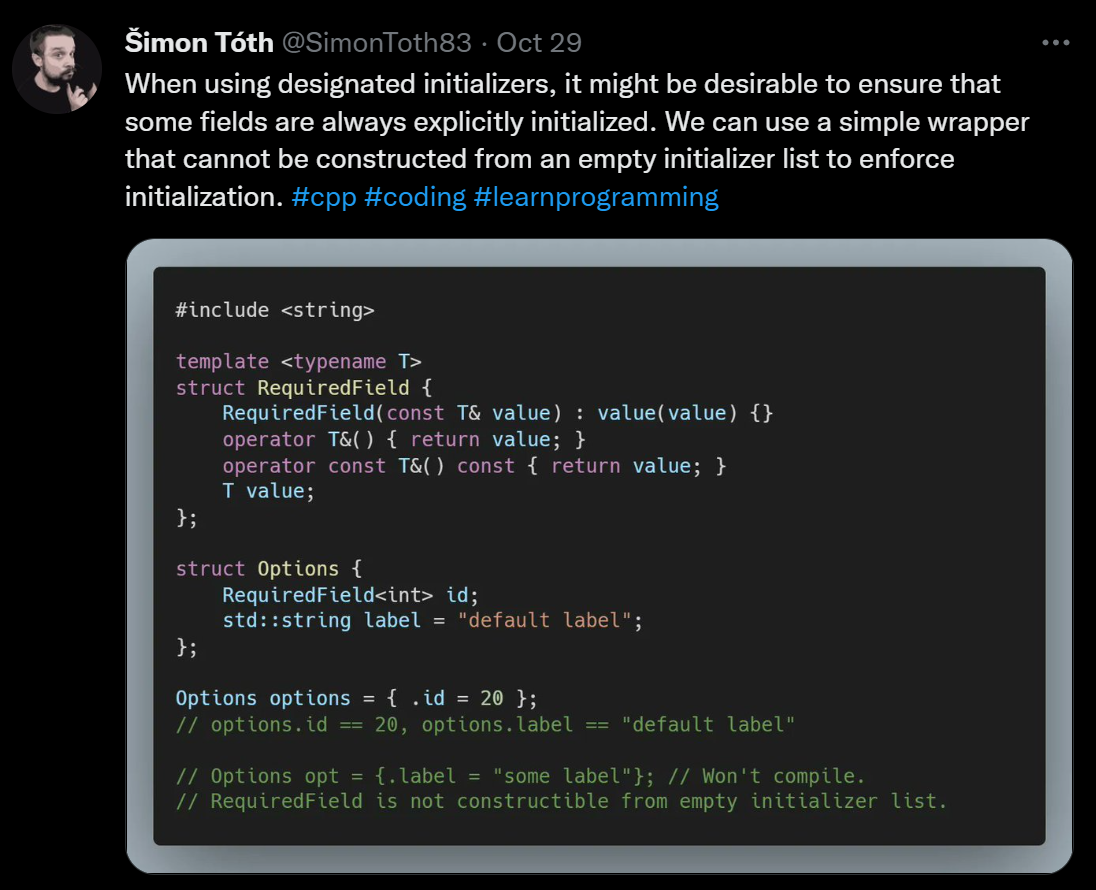
\includegraphics[width=\textwidth]{static/tweet.png}
    \end{column}
\end{columns}
\end{frame}

\begin{frame}{}
\begin{center}
    \begin{Huge}
        Monorepo vs Polyrepo
    \end{Huge}
\end{center}
\end{frame}

\begin{frame}{}
\Huge
\begin{center}
\begin{description}
    \item[mono-] one, single \pause
    \item[poly-] many
\end{description}
\end{center}
\end{frame}

\begin{frame}{}
\Huge
\begin{center}
\begin{description}
    \item[@HEAD] built from current sources \pause
    \item[binary] versioned binaries
\end{description}
\end{center}
\end{frame}

\begin{frame}{Comparison}
\begin{columns}
    \begin{column}{0.5\textwidth}
    @HEAD monorepo
    \begin{itemize}
        \item<2-> \emoji{face-with-head-bandage} scalability 
        \item<3-> \emoji{smirking-face} global operations are possible
        \item<4-> \emoji{grimacing-face} private dependencies are non-trivial
        \item<5-> \emoji{face-with-raised-eyebrow} shared dependencies need to be carefully managed
    \end{itemize}
    \end{column}
    \begin{column}{0.5\textwidth}
    binary polyrepo
    \begin{itemize}
        \item<2-> \emoji{anxious-face-with-sweat} ABI stability
        \item<3-> \emoji{exploding-head} global operations do not exist
        \item<4-> \emoji{smiling-face-with-smiling-eyes} private dependencies are trivial
        \item<5-> \emoji{frowning-face} shared dependencies need to be carefully managed
    \end{itemize}
    \end{column}
\end{columns}
\end{frame}

\begin{frame}{Comparison}
\begin{columns}
    \begin{column}{0.5\textwidth}
    @HEAD monorepo
    \begin{itemize}
        \item<2-> cooperative
        \item<3-> conforming
        \item<4-> biased towards users
    \end{itemize}
    \end{column}
    \begin{column}{0.5\textwidth}
    binary polyrepo
    \begin{itemize}
        \item<2-> competitive
        \item<3-> independent
        \item<4-> biased towards providers
    \end{itemize}
    \end{column}
\end{columns}
\end{frame}

\begin{frame}{}
\begin{center}
    \begin{Huge}
        Bazel
    \end{Huge}
\end{center}
\end{frame}

\begin{frame}{}
    \begin{center}
        \begin{Huge}Hello World Demo\end{Huge}
    \end{center}
\end{frame}

{
\usebackgroundtemplate{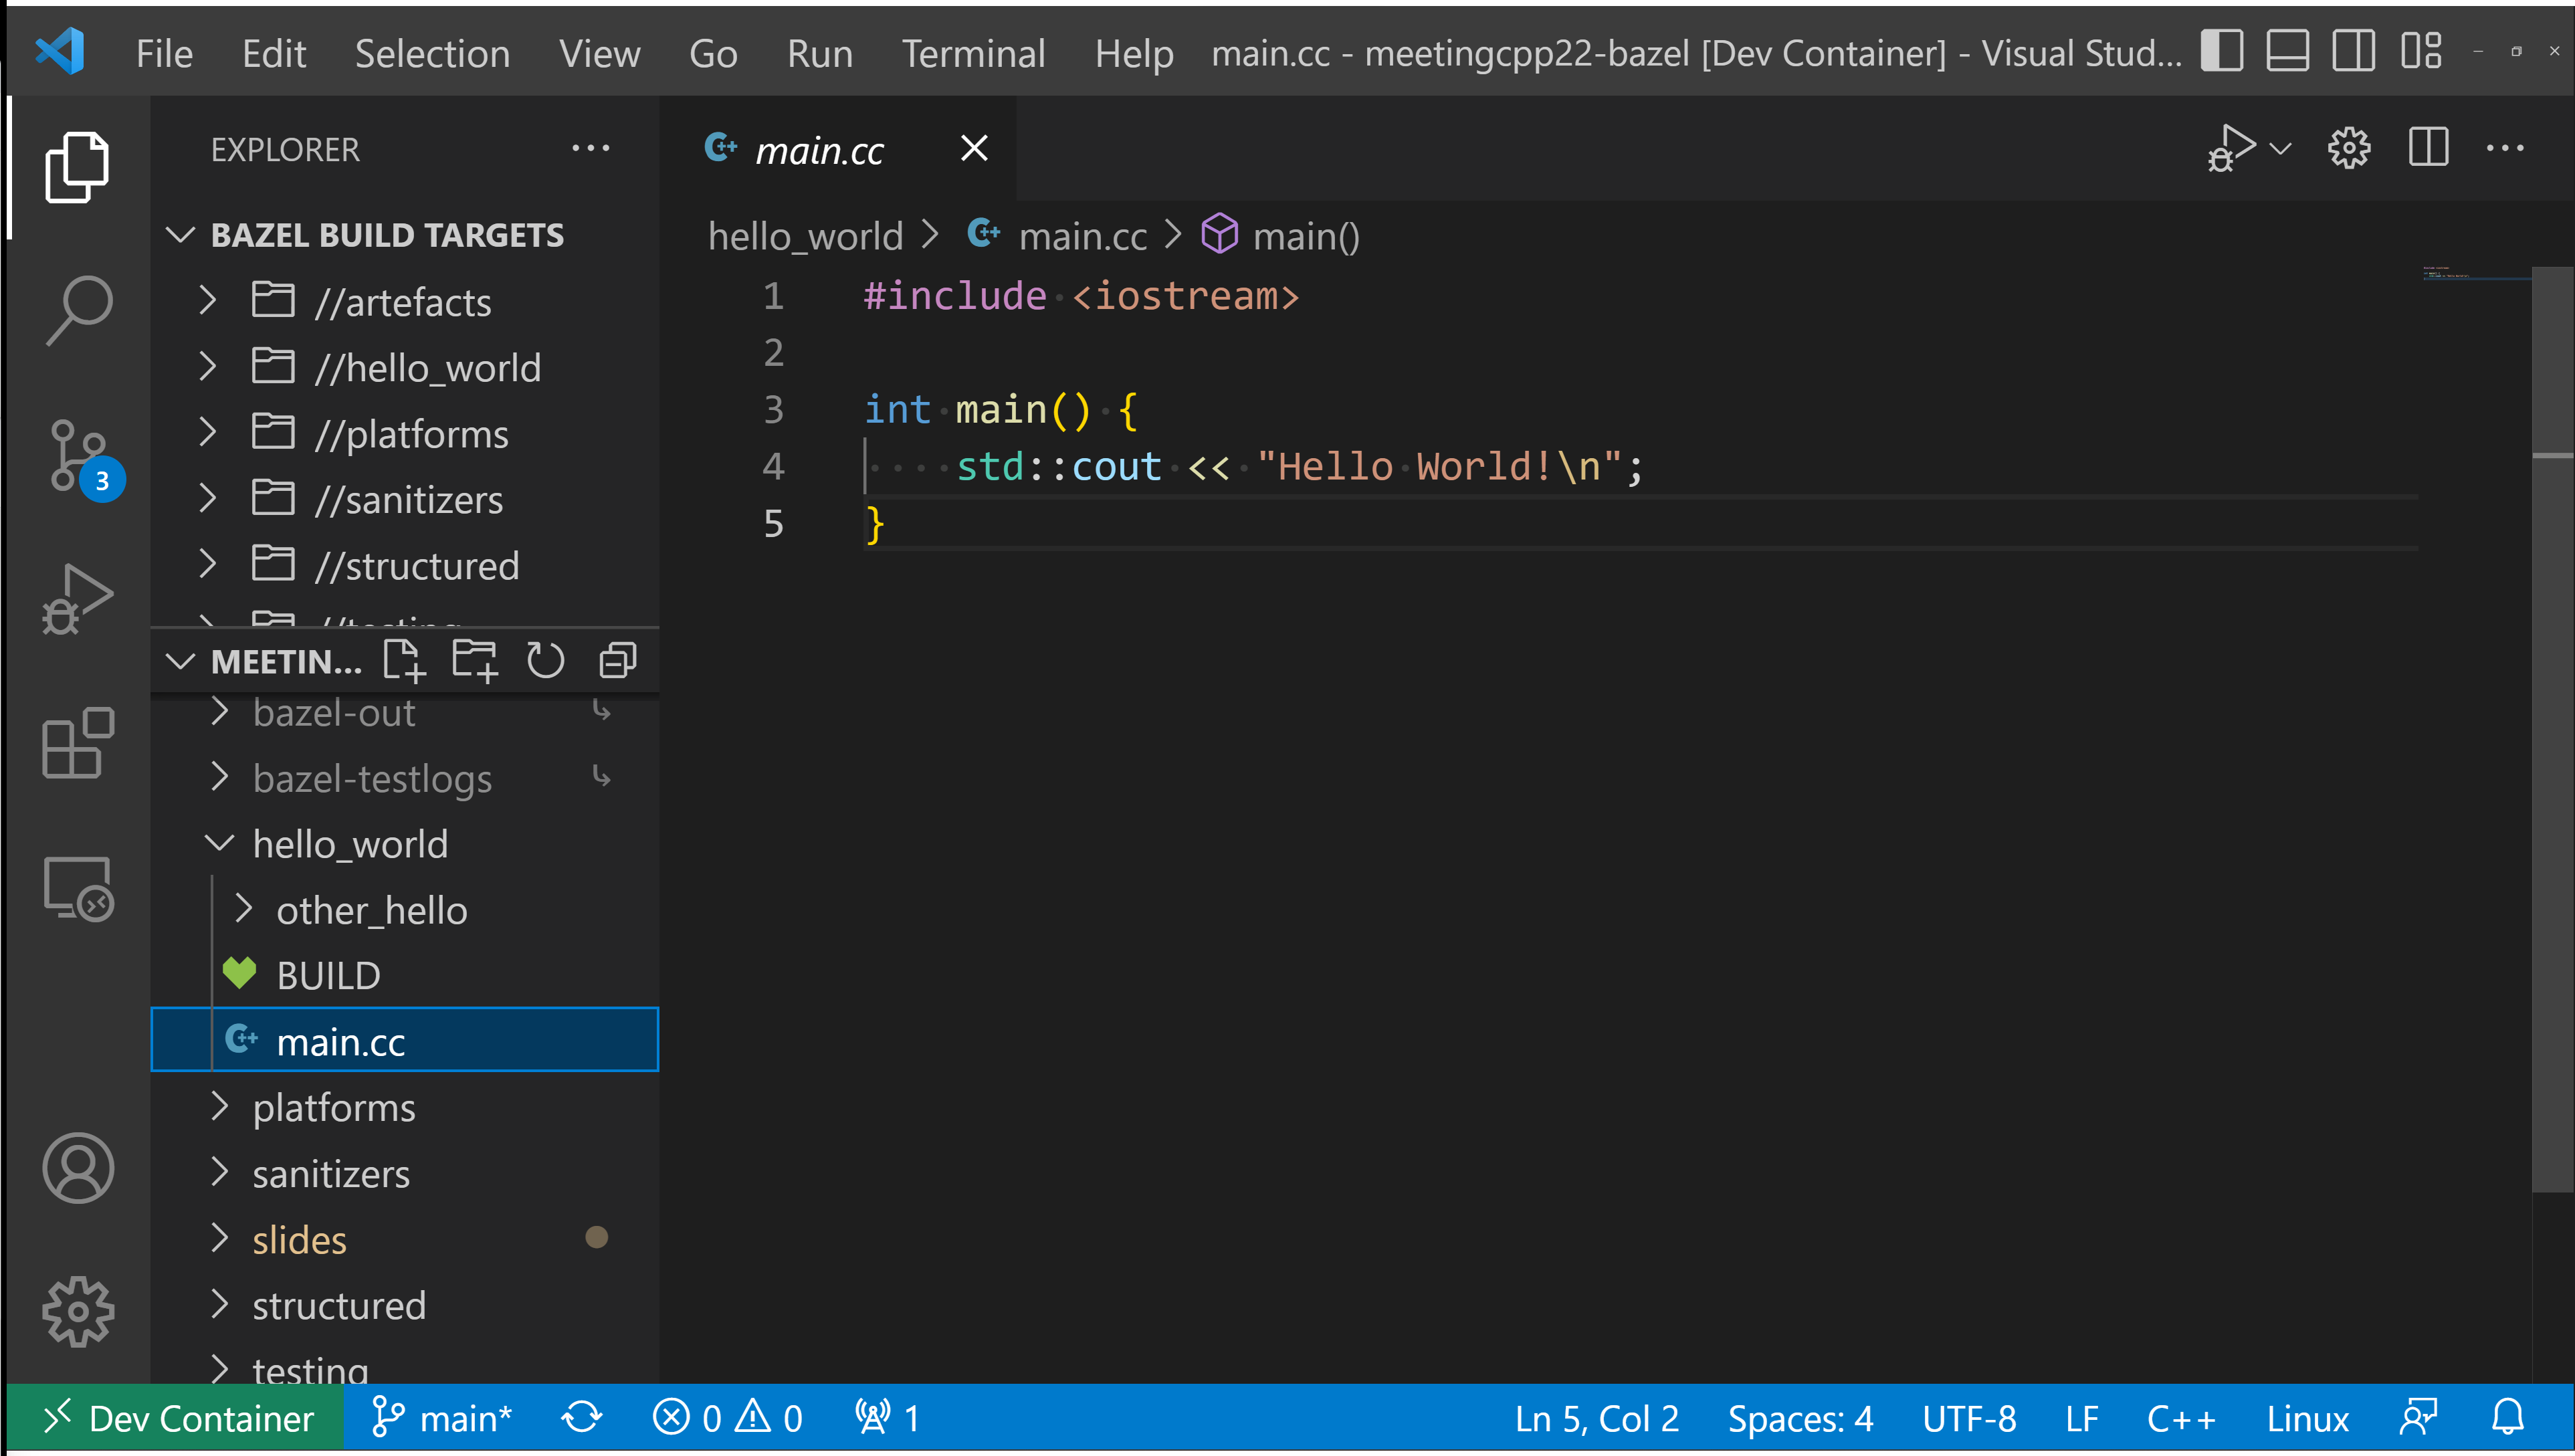
\includegraphics[width=\paperwidth]{slides/static_demos/00_01_hello_world.png}}
\begin{frame}[plain]
\end{frame}
}

{
\usebackgroundtemplate{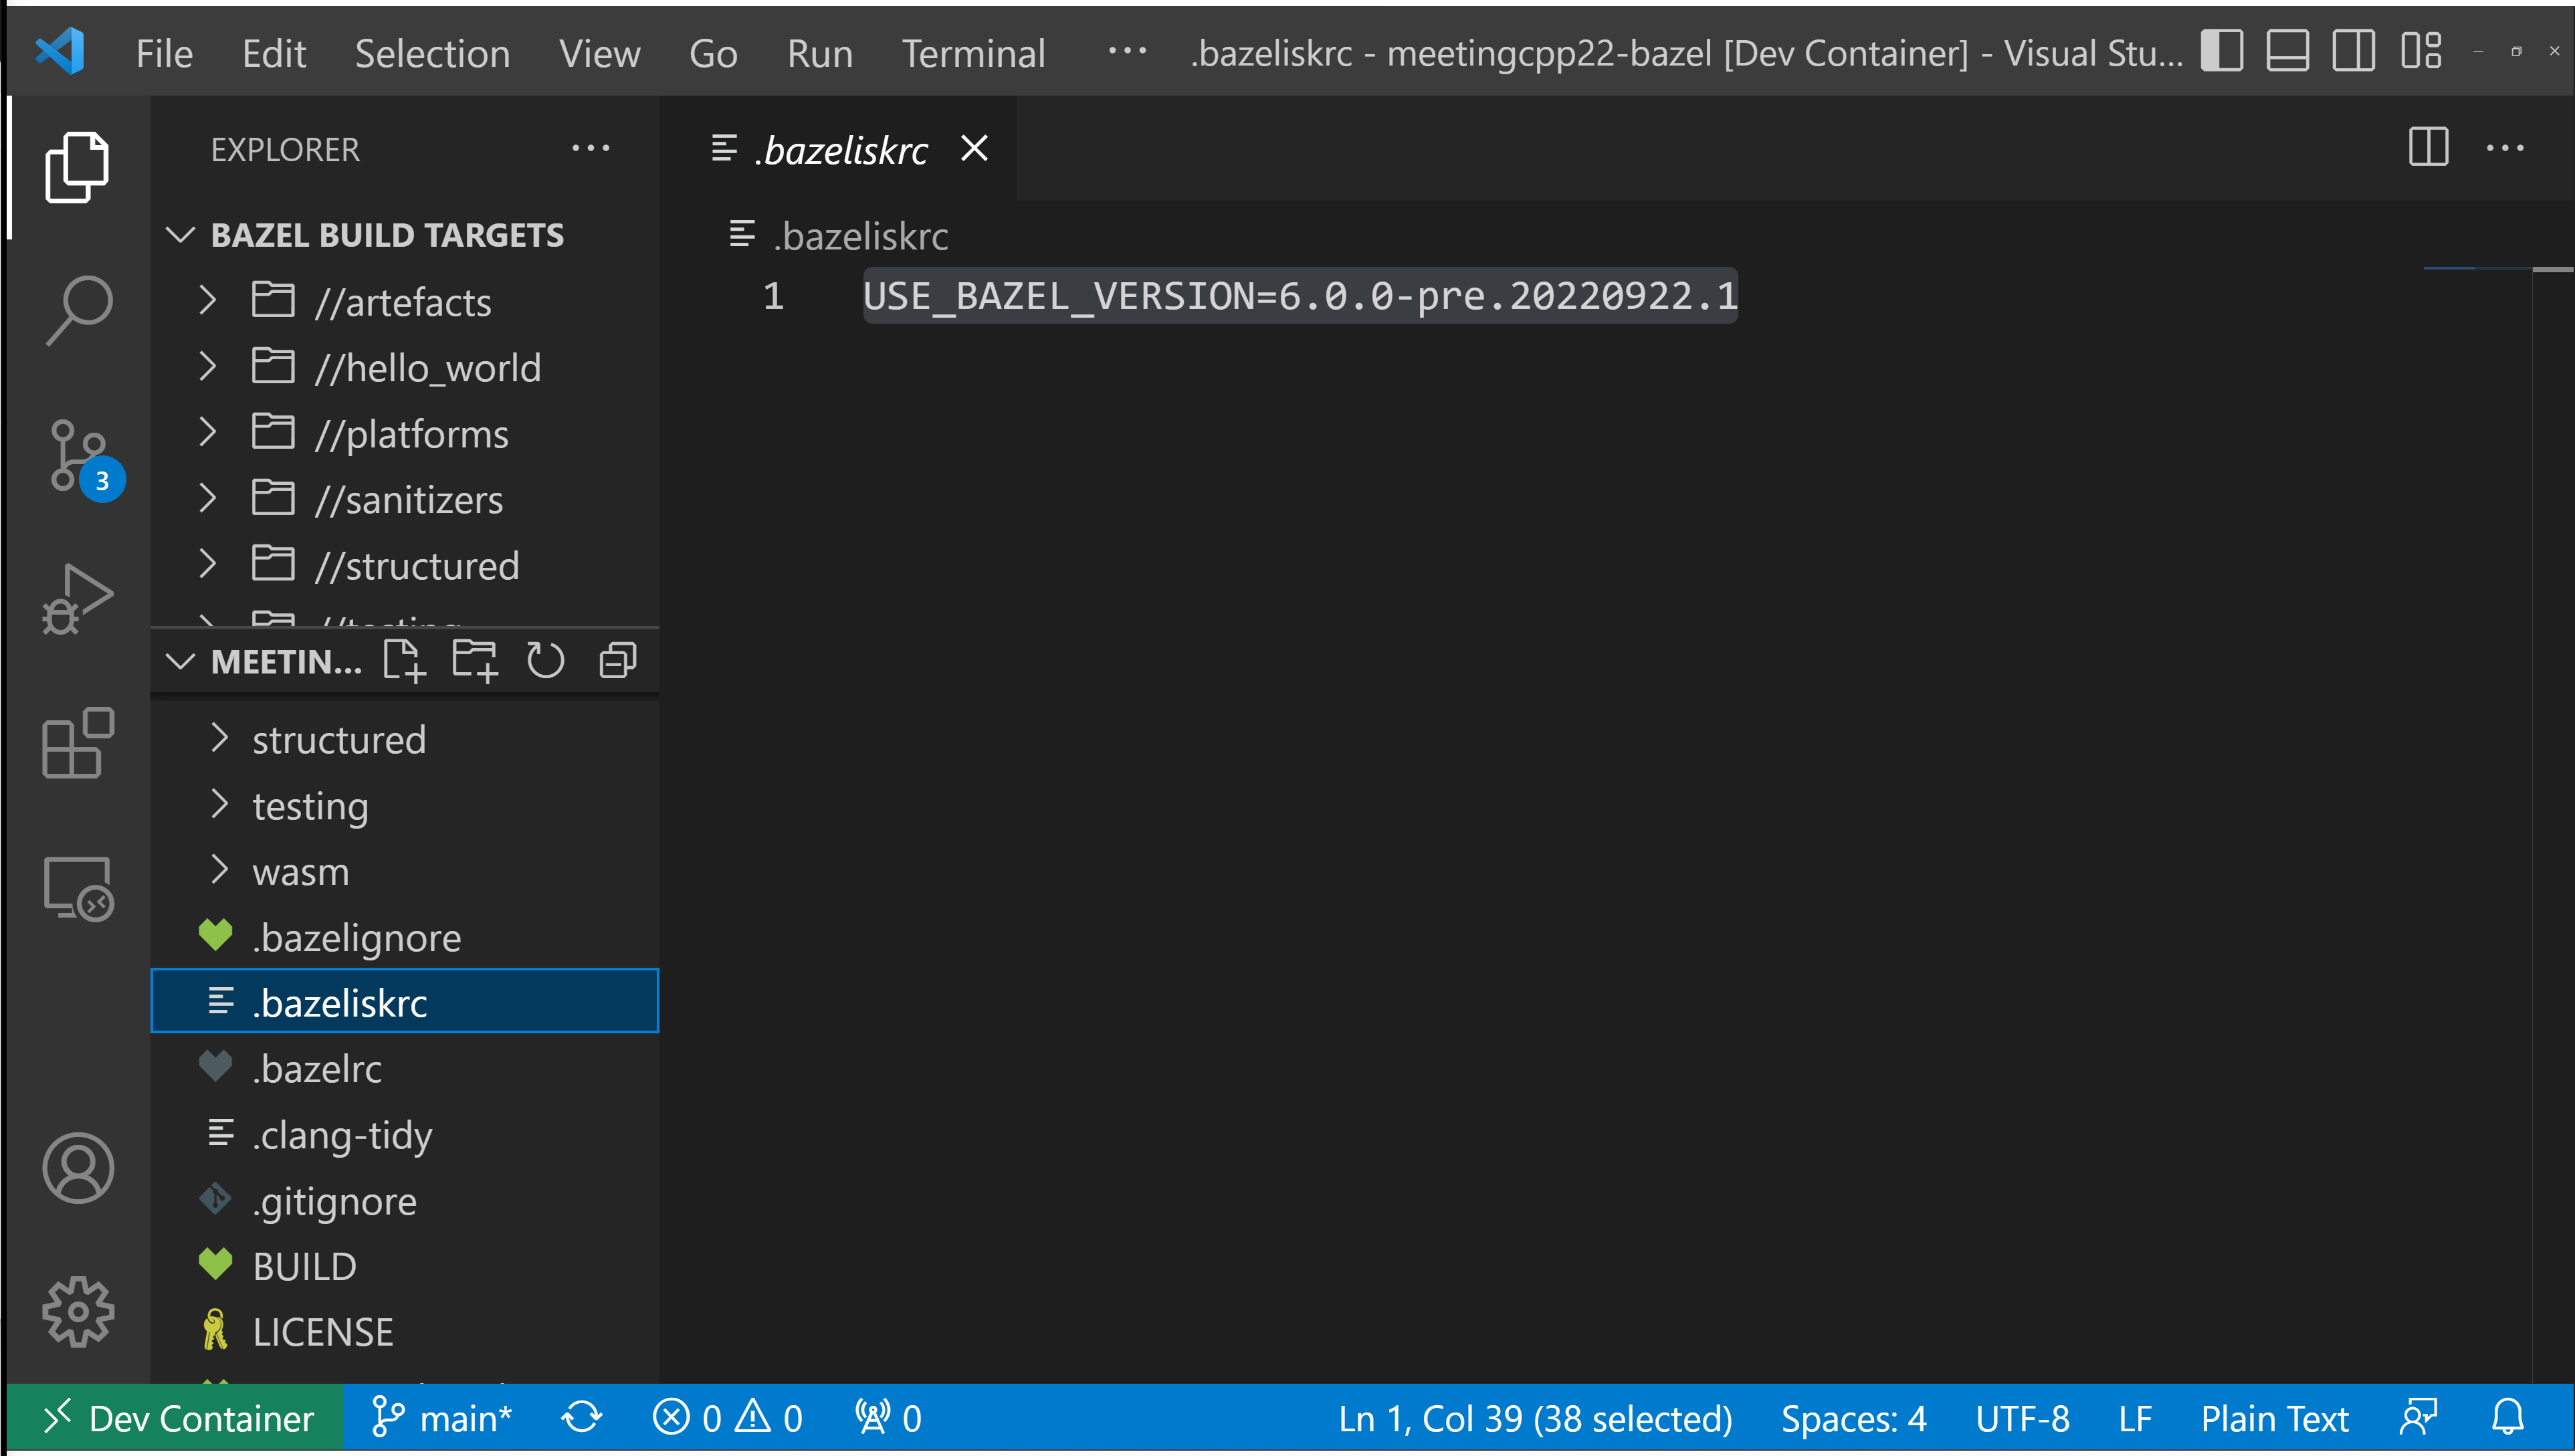
\includegraphics[width=\paperwidth]{slides/static_demos/00_02_bazeliskrc.png}}
\begin{frame}[plain]
\end{frame}
}

{
\usebackgroundtemplate{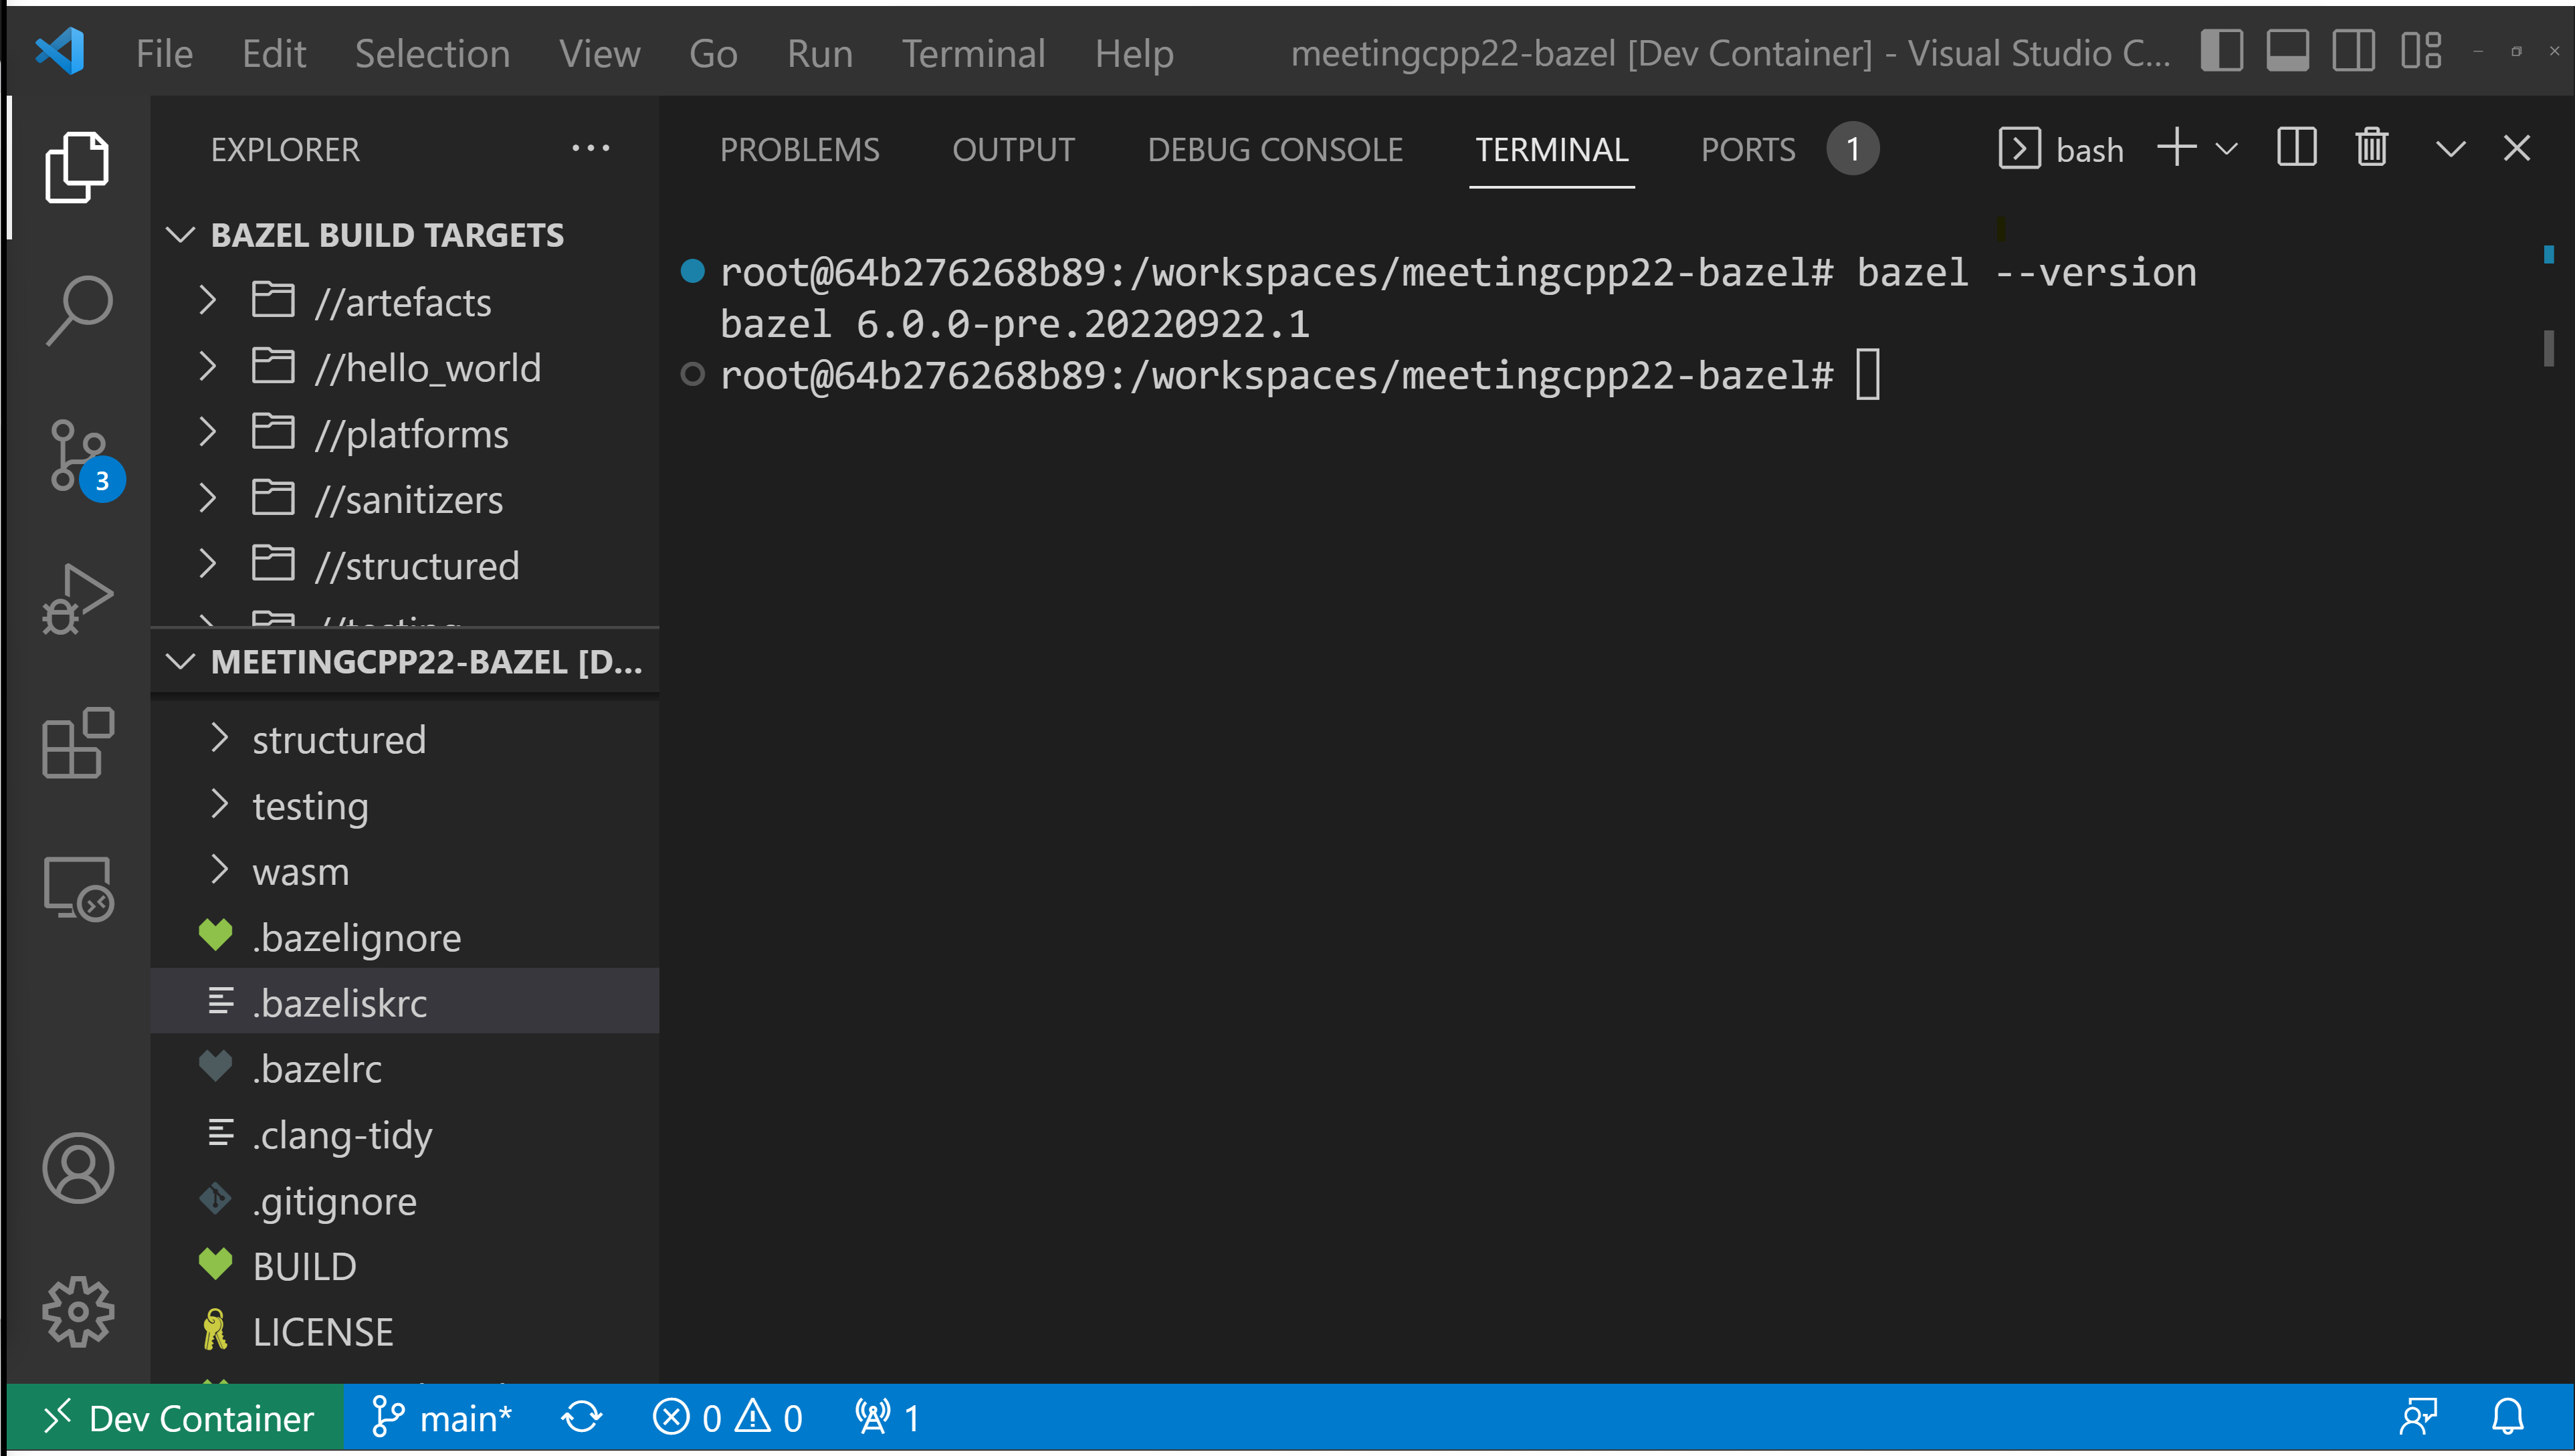
\includegraphics[width=\paperwidth]{slides/static_demos/00_03_bazel_version.png}}
\begin{frame}[plain]
\end{frame}
}

{
\usebackgroundtemplate{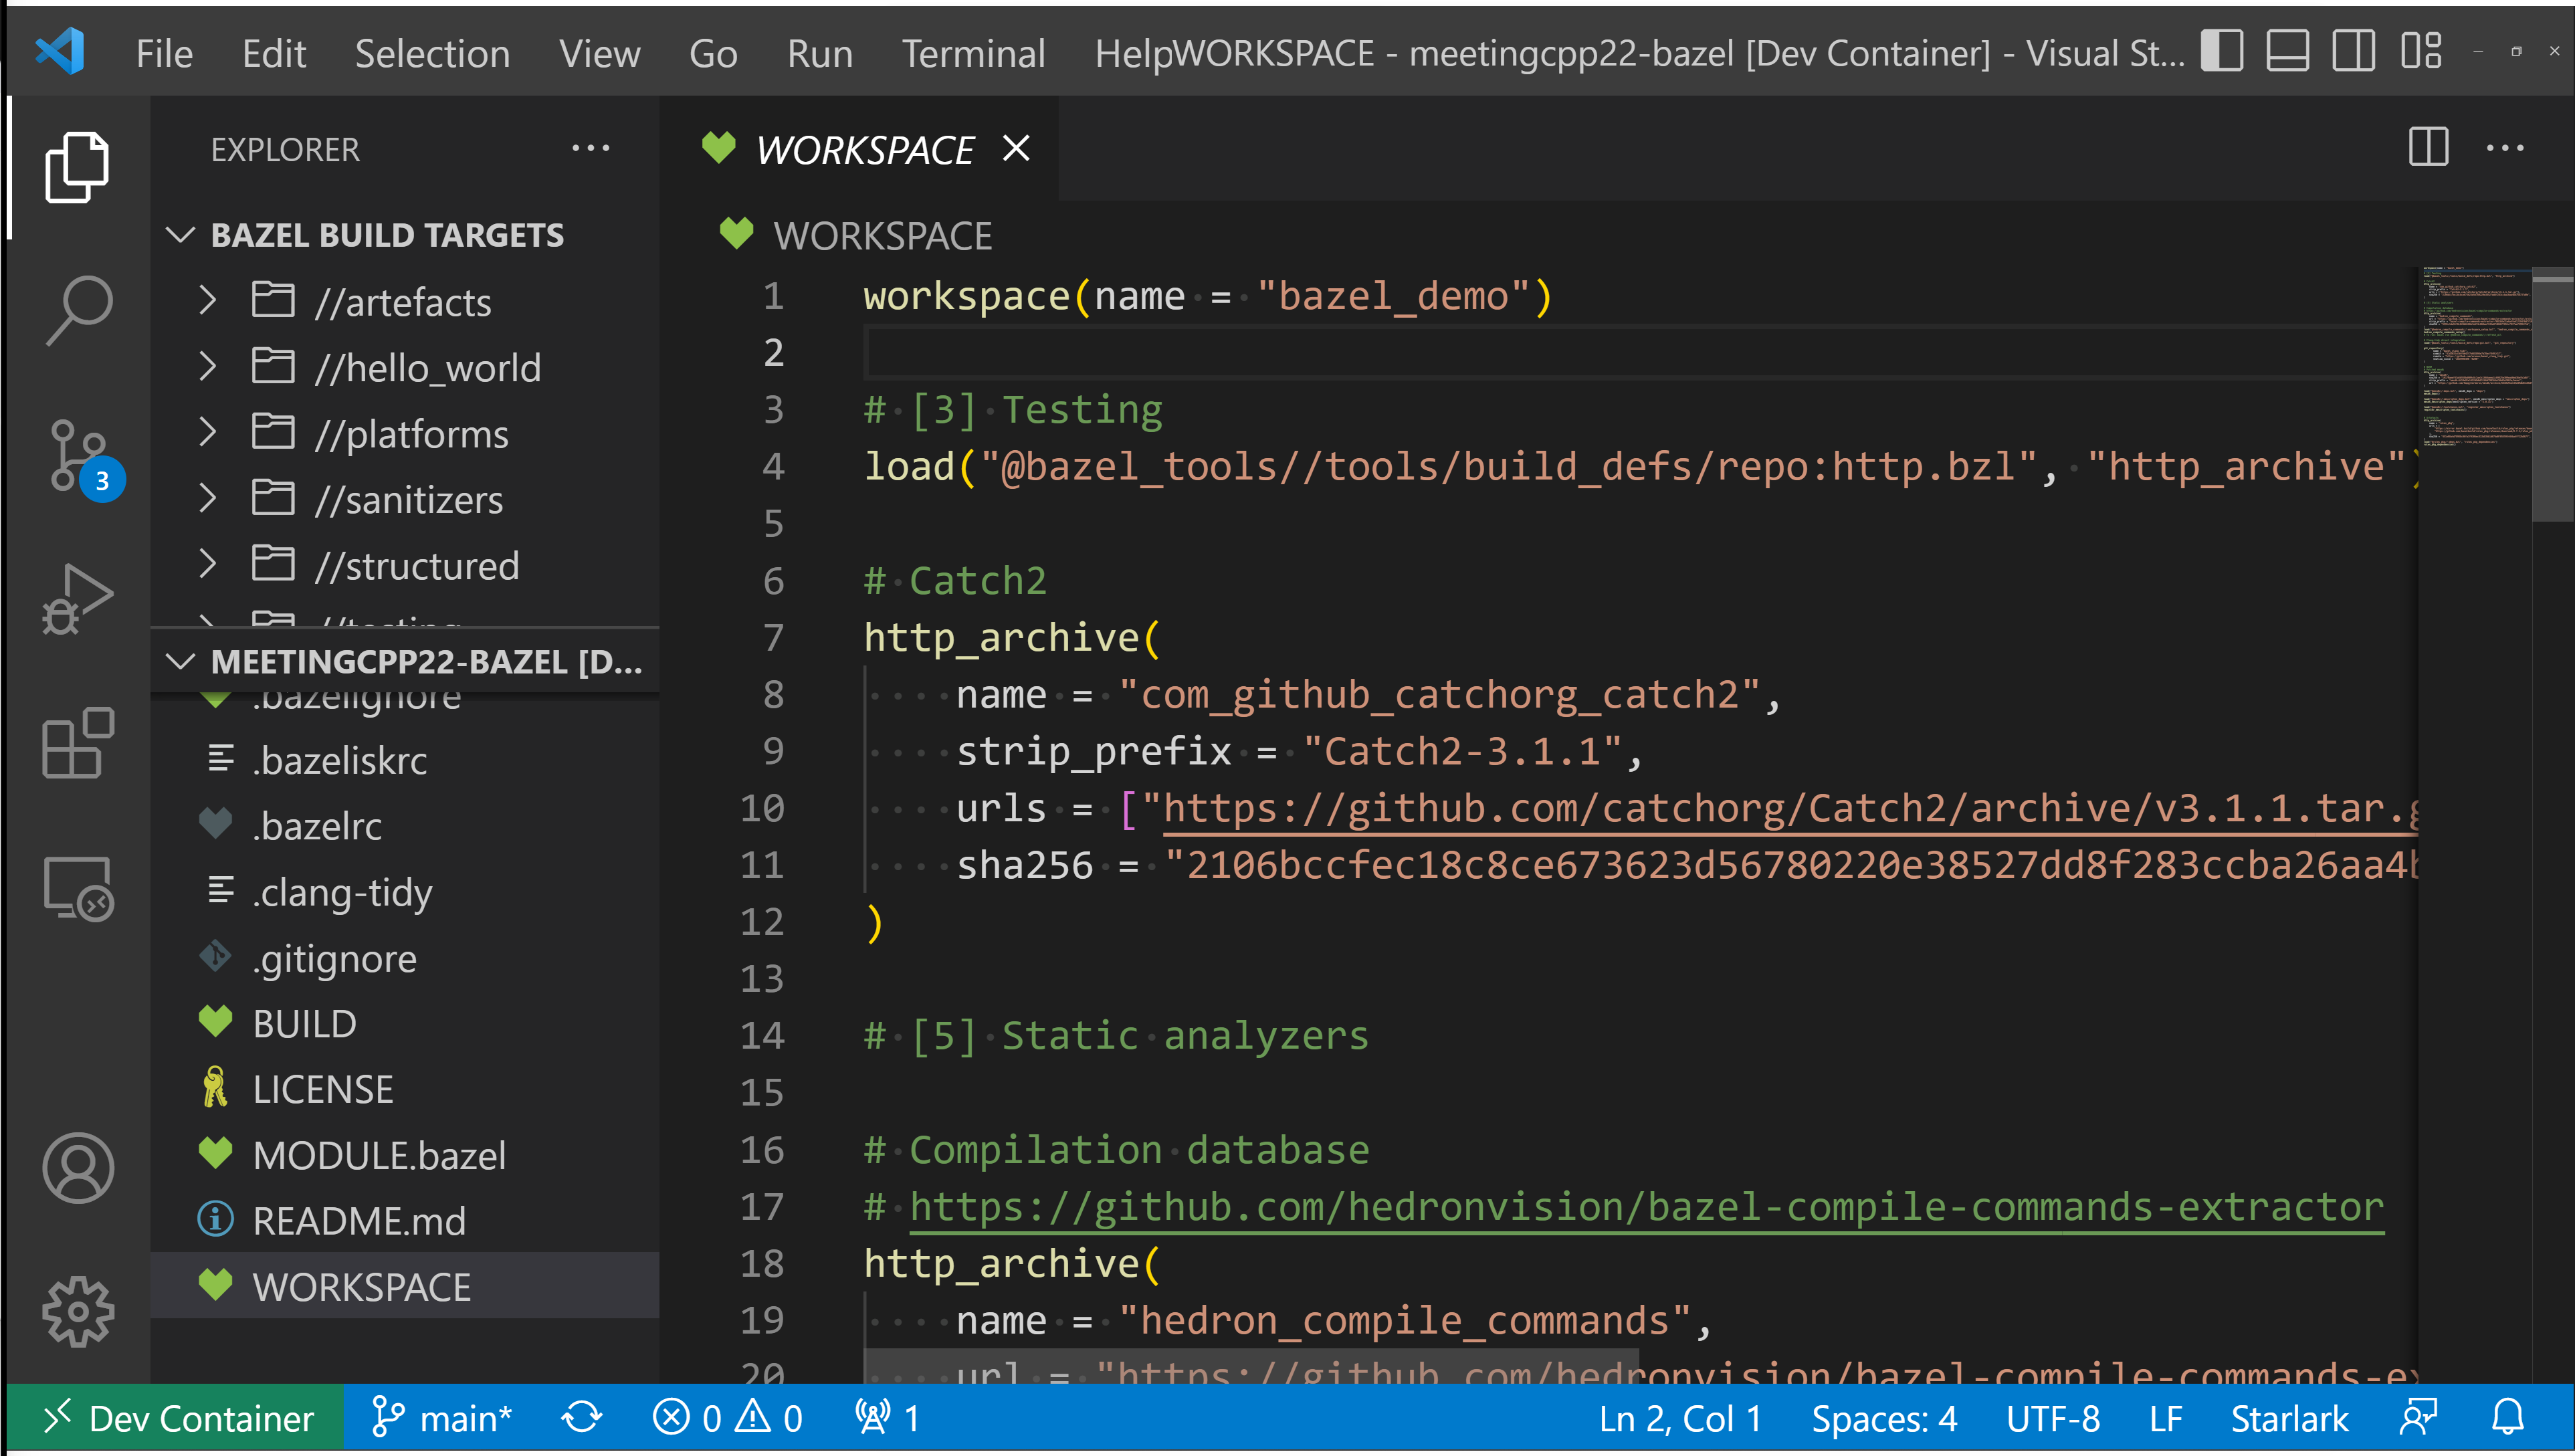
\includegraphics[width=\paperwidth]{slides/static_demos/00_04_WORKSPACE.png}}
\begin{frame}[plain]
\end{frame}
}

{
\usebackgroundtemplate{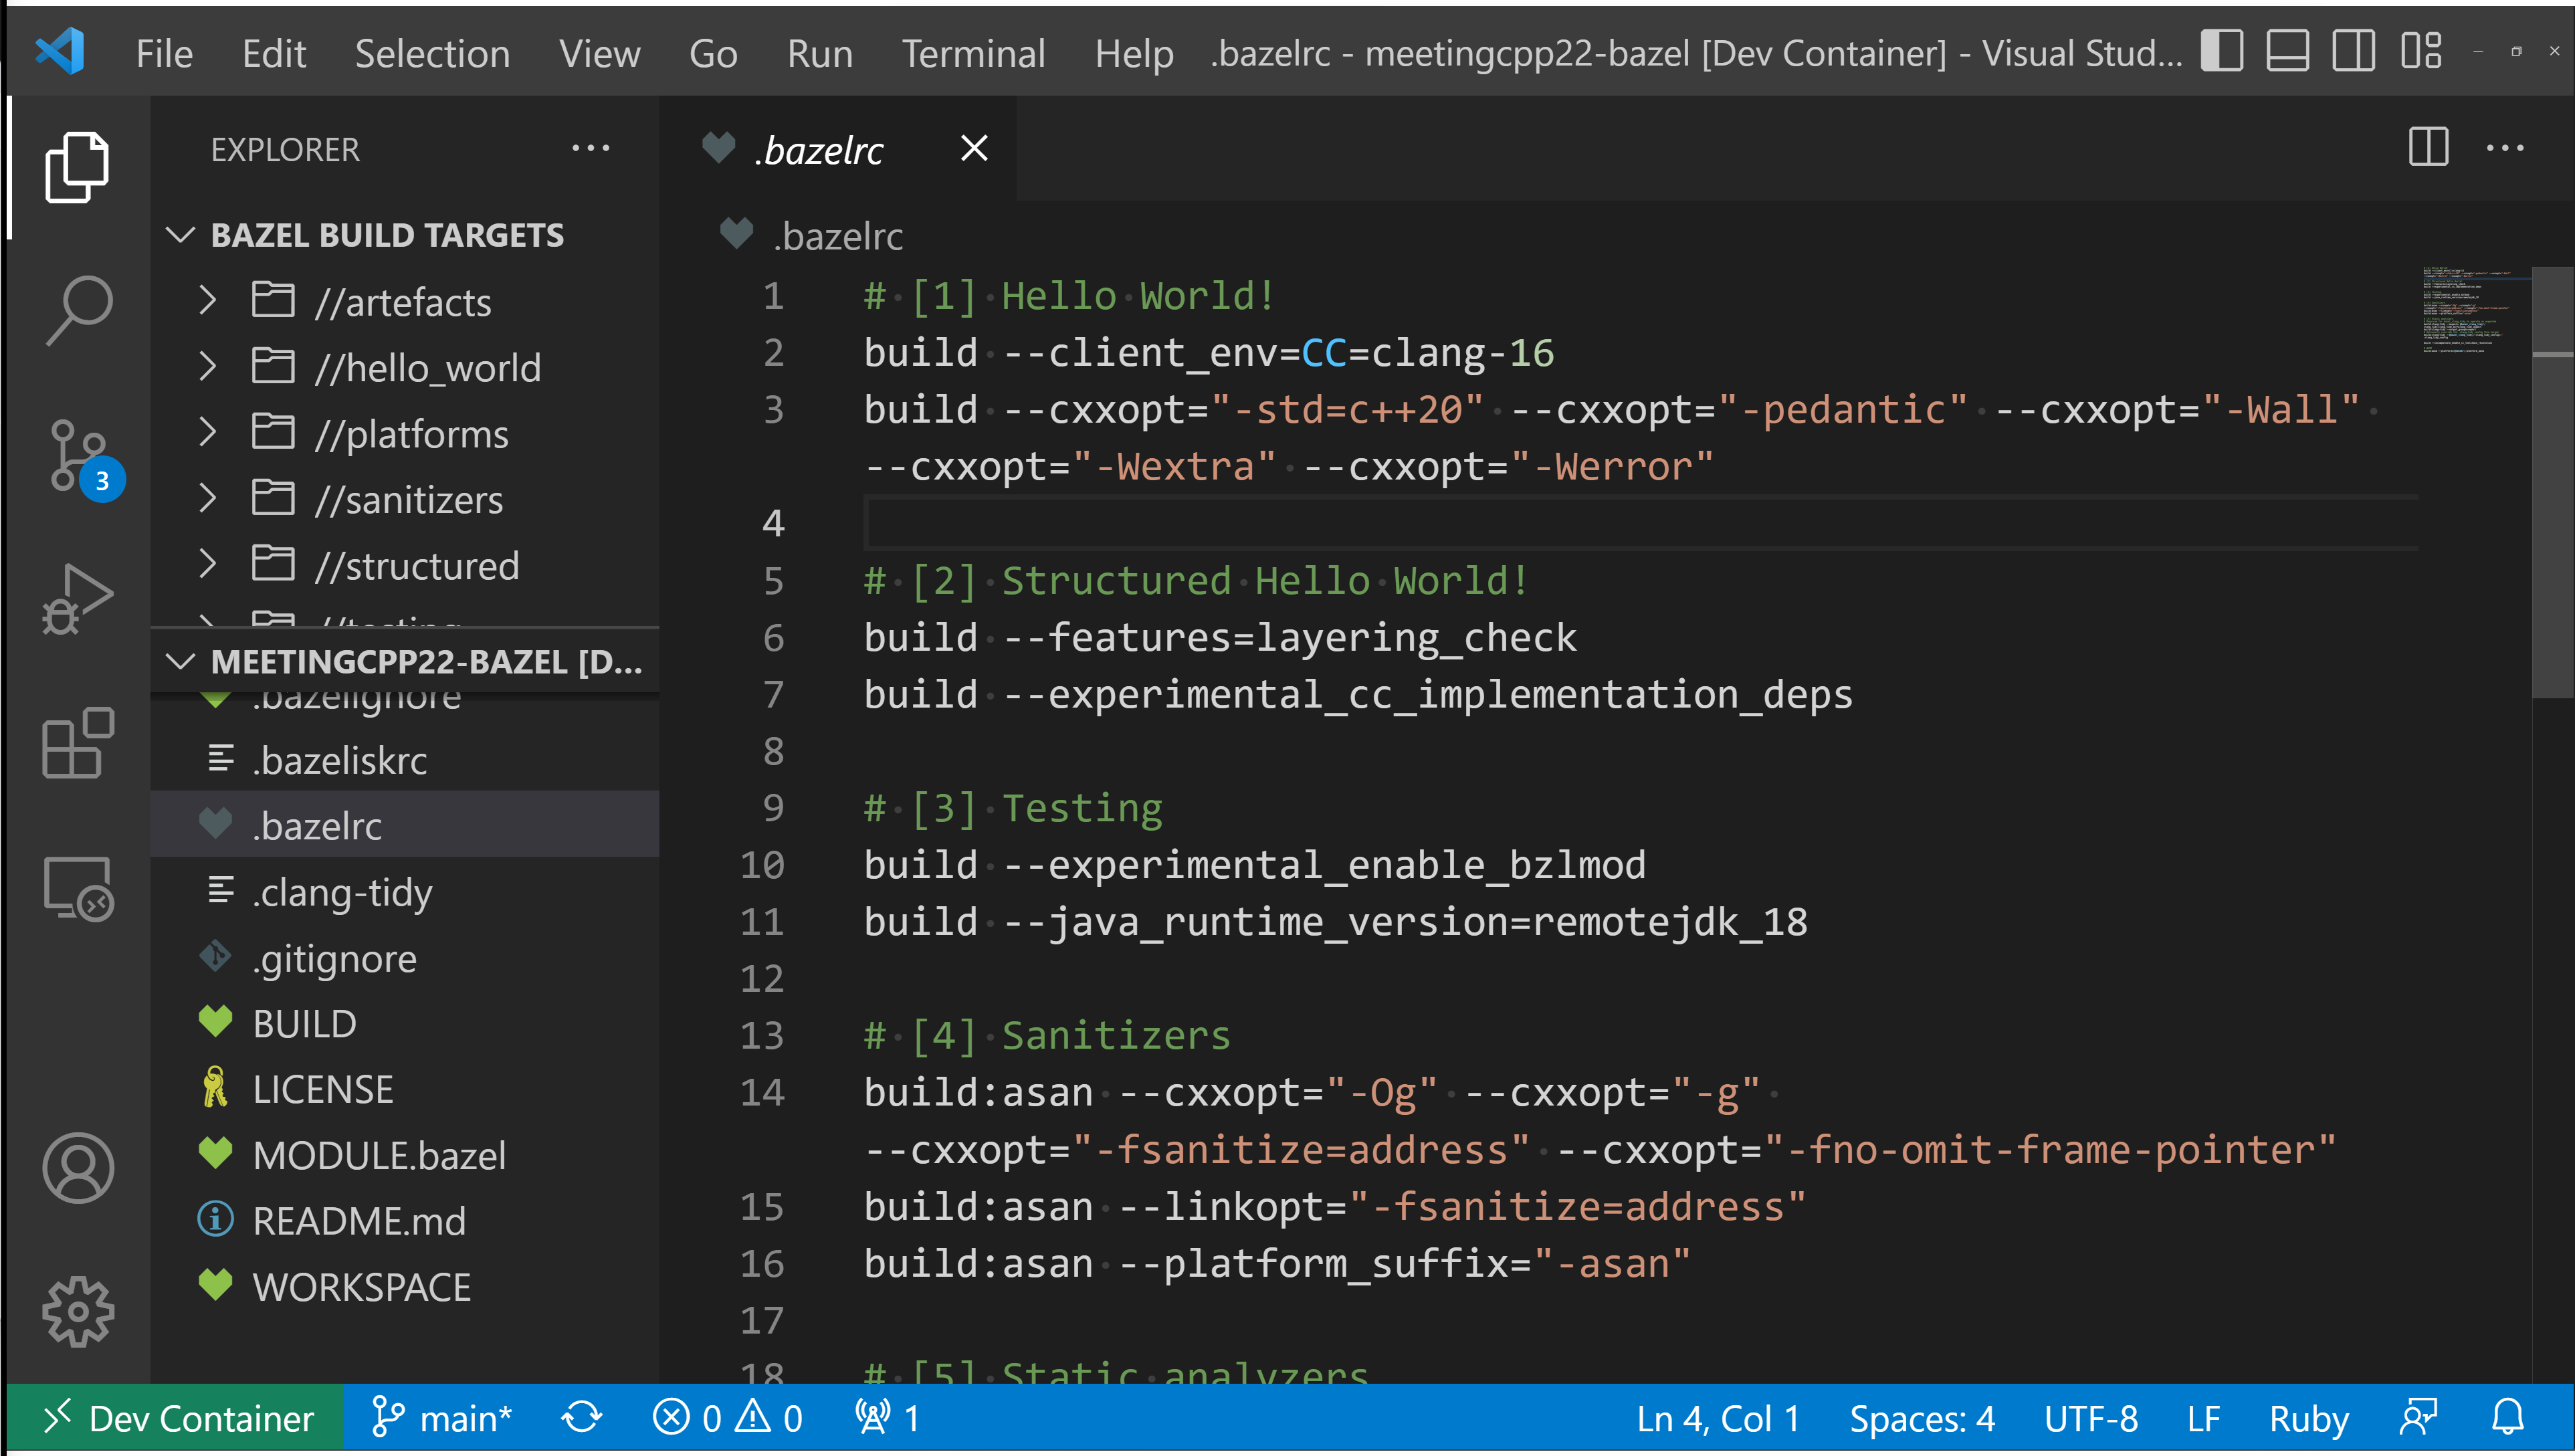
\includegraphics[width=\paperwidth]{slides/static_demos/00_05_bazelrc.png}}
\begin{frame}[plain]
\end{frame}
}

{
\usebackgroundtemplate{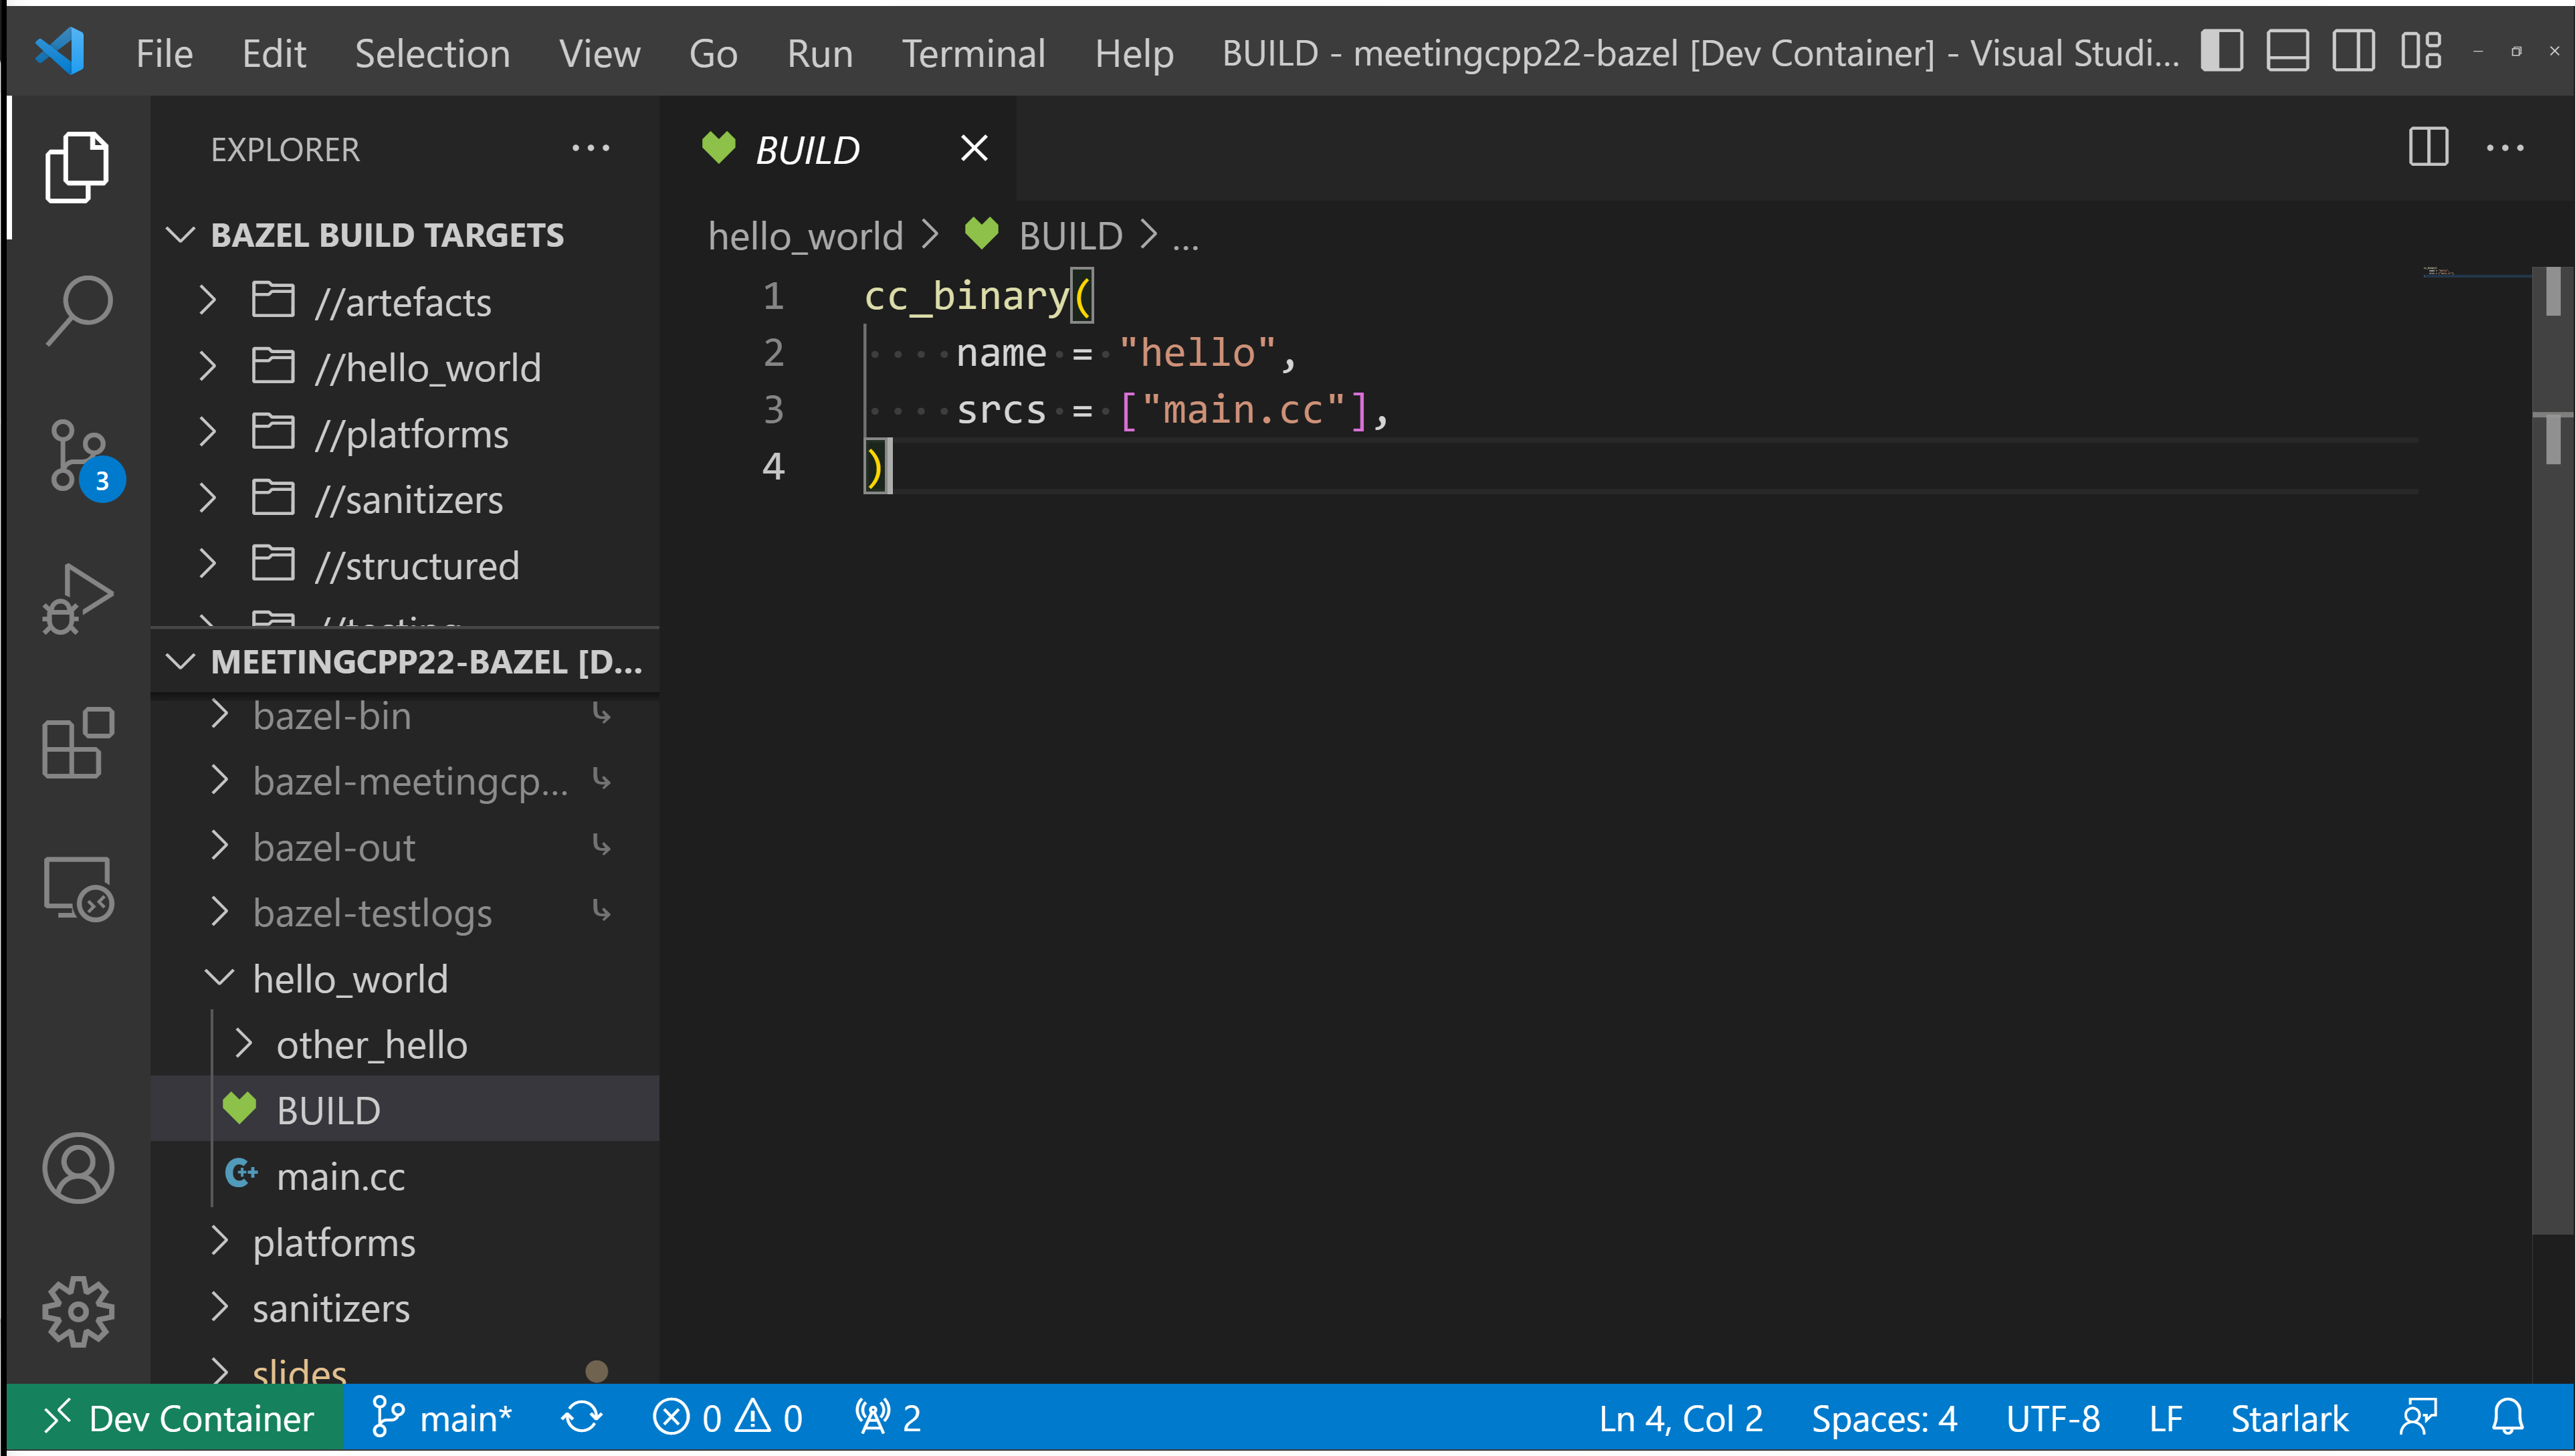
\includegraphics[width=\paperwidth]{slides/static_demos/00_06_BUILD.png}}
\begin{frame}[plain]
\end{frame}
}

{
\usebackgroundtemplate{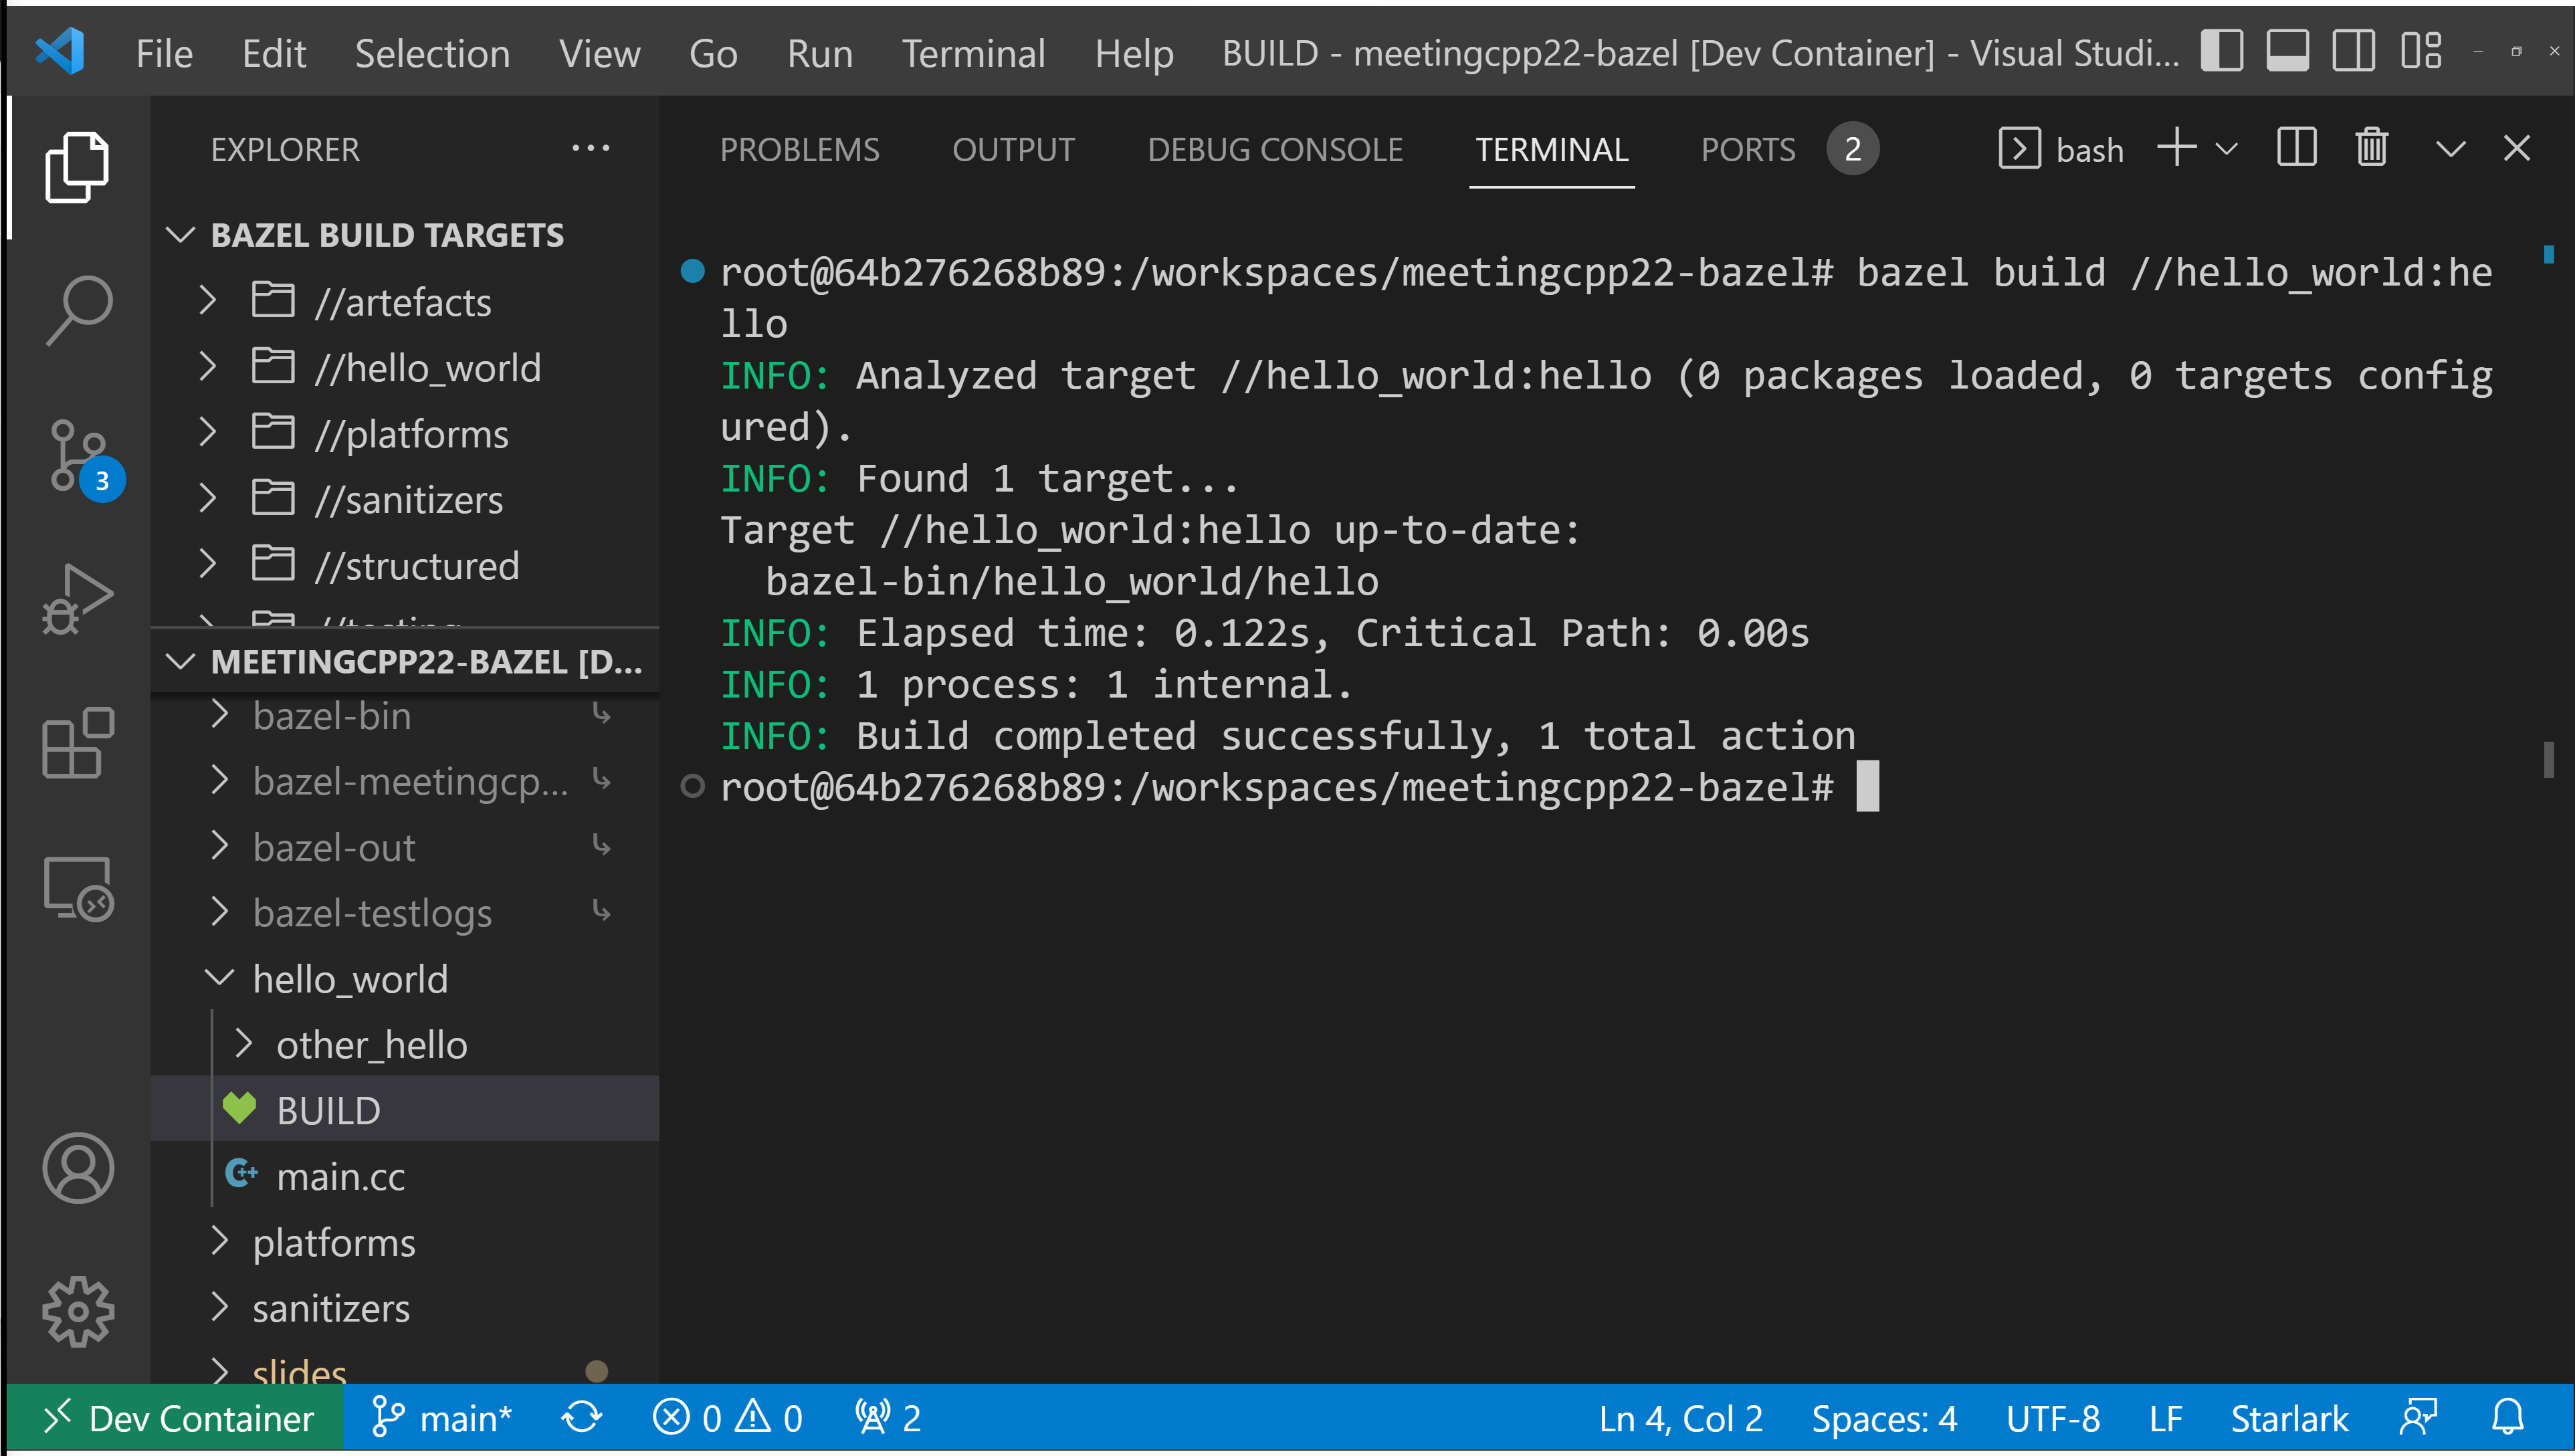
\includegraphics[width=\paperwidth]{slides/static_demos/00_07_build.png}}
\begin{frame}[plain]
\end{frame}
}

{
\usebackgroundtemplate{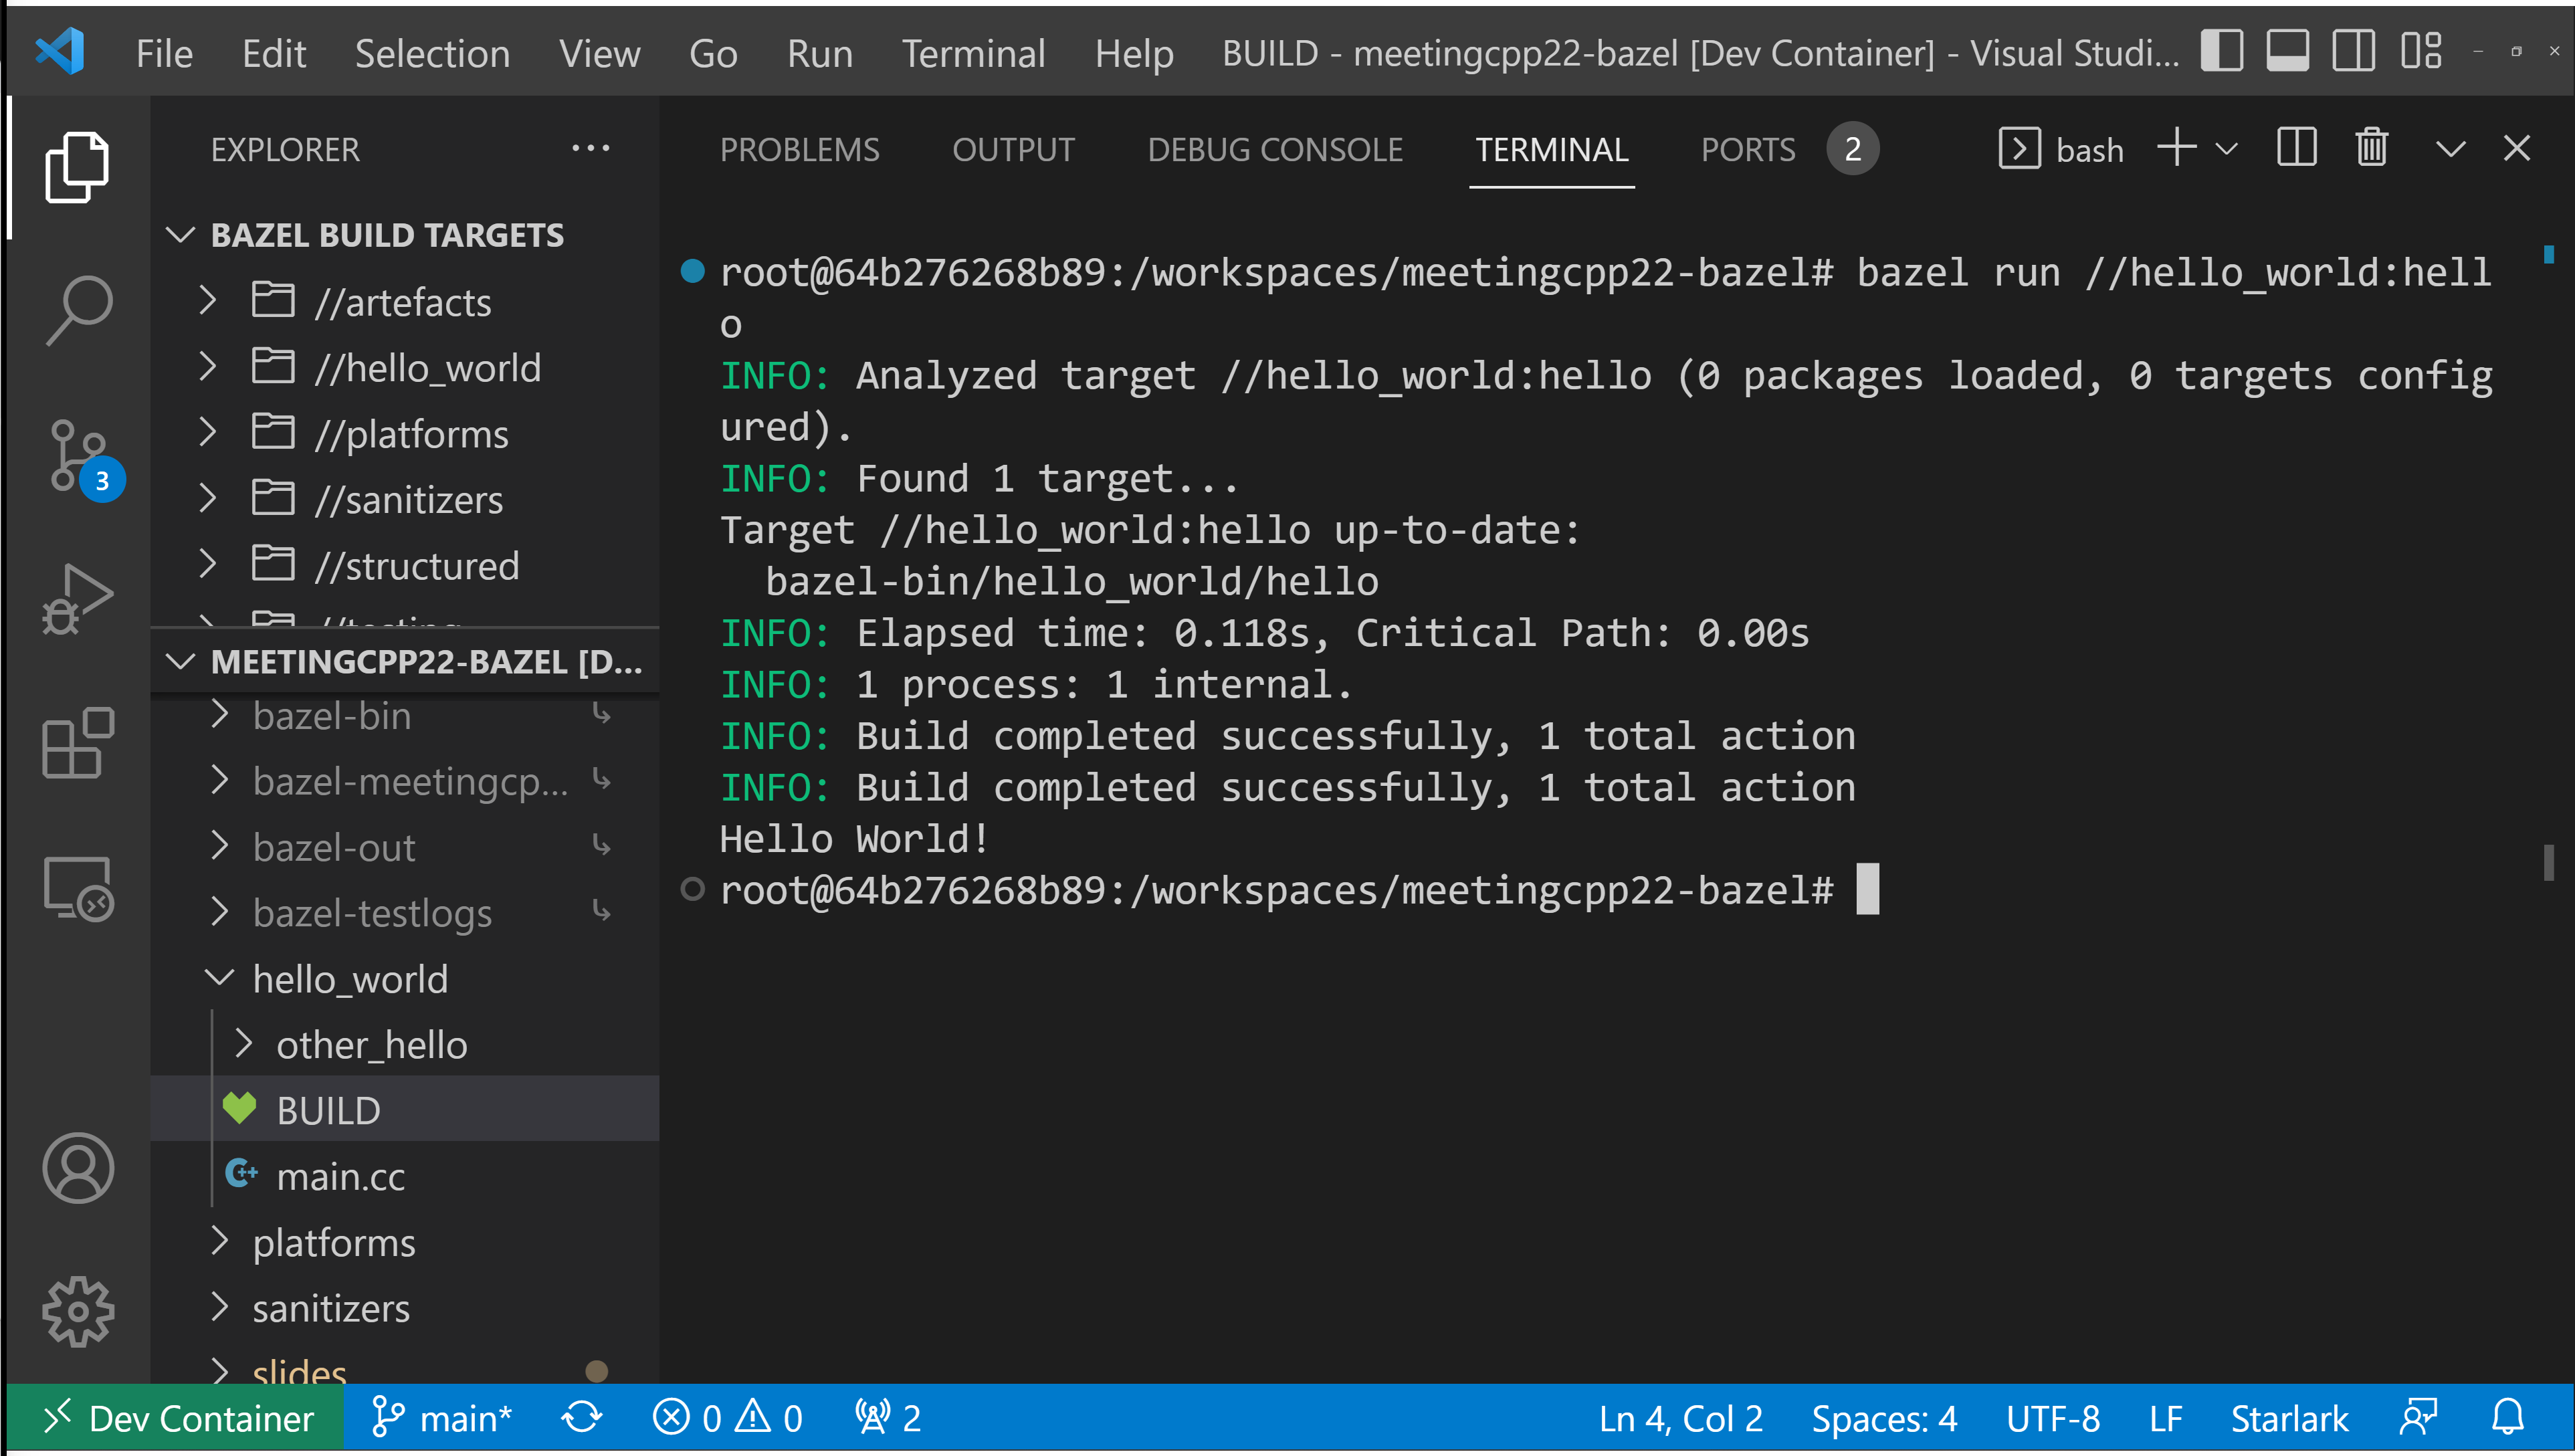
\includegraphics[width=\paperwidth]{slides/static_demos/00_08_run.png}}
\begin{frame}[plain]
\end{frame}
}

\begin{frame}{Repo, Package, Target}
\begin{center}
\begin{overprint}
\onslide<1> \huge{\texttt{@repo//package/path:target}}
\onslide<2> \huge{\texttt{@//package/path:target}}
\onslide<3>\huge{\texttt{//package/path:target}}
\onslide<4>\huge{\texttt{:target}}
\onslide<5>\huge{\texttt{//package/path:path}}
\onslide<6>\huge{\texttt{//package/path}}
\end{overprint}
\end{center}
\end{frame}

{
\usebackgroundtemplate{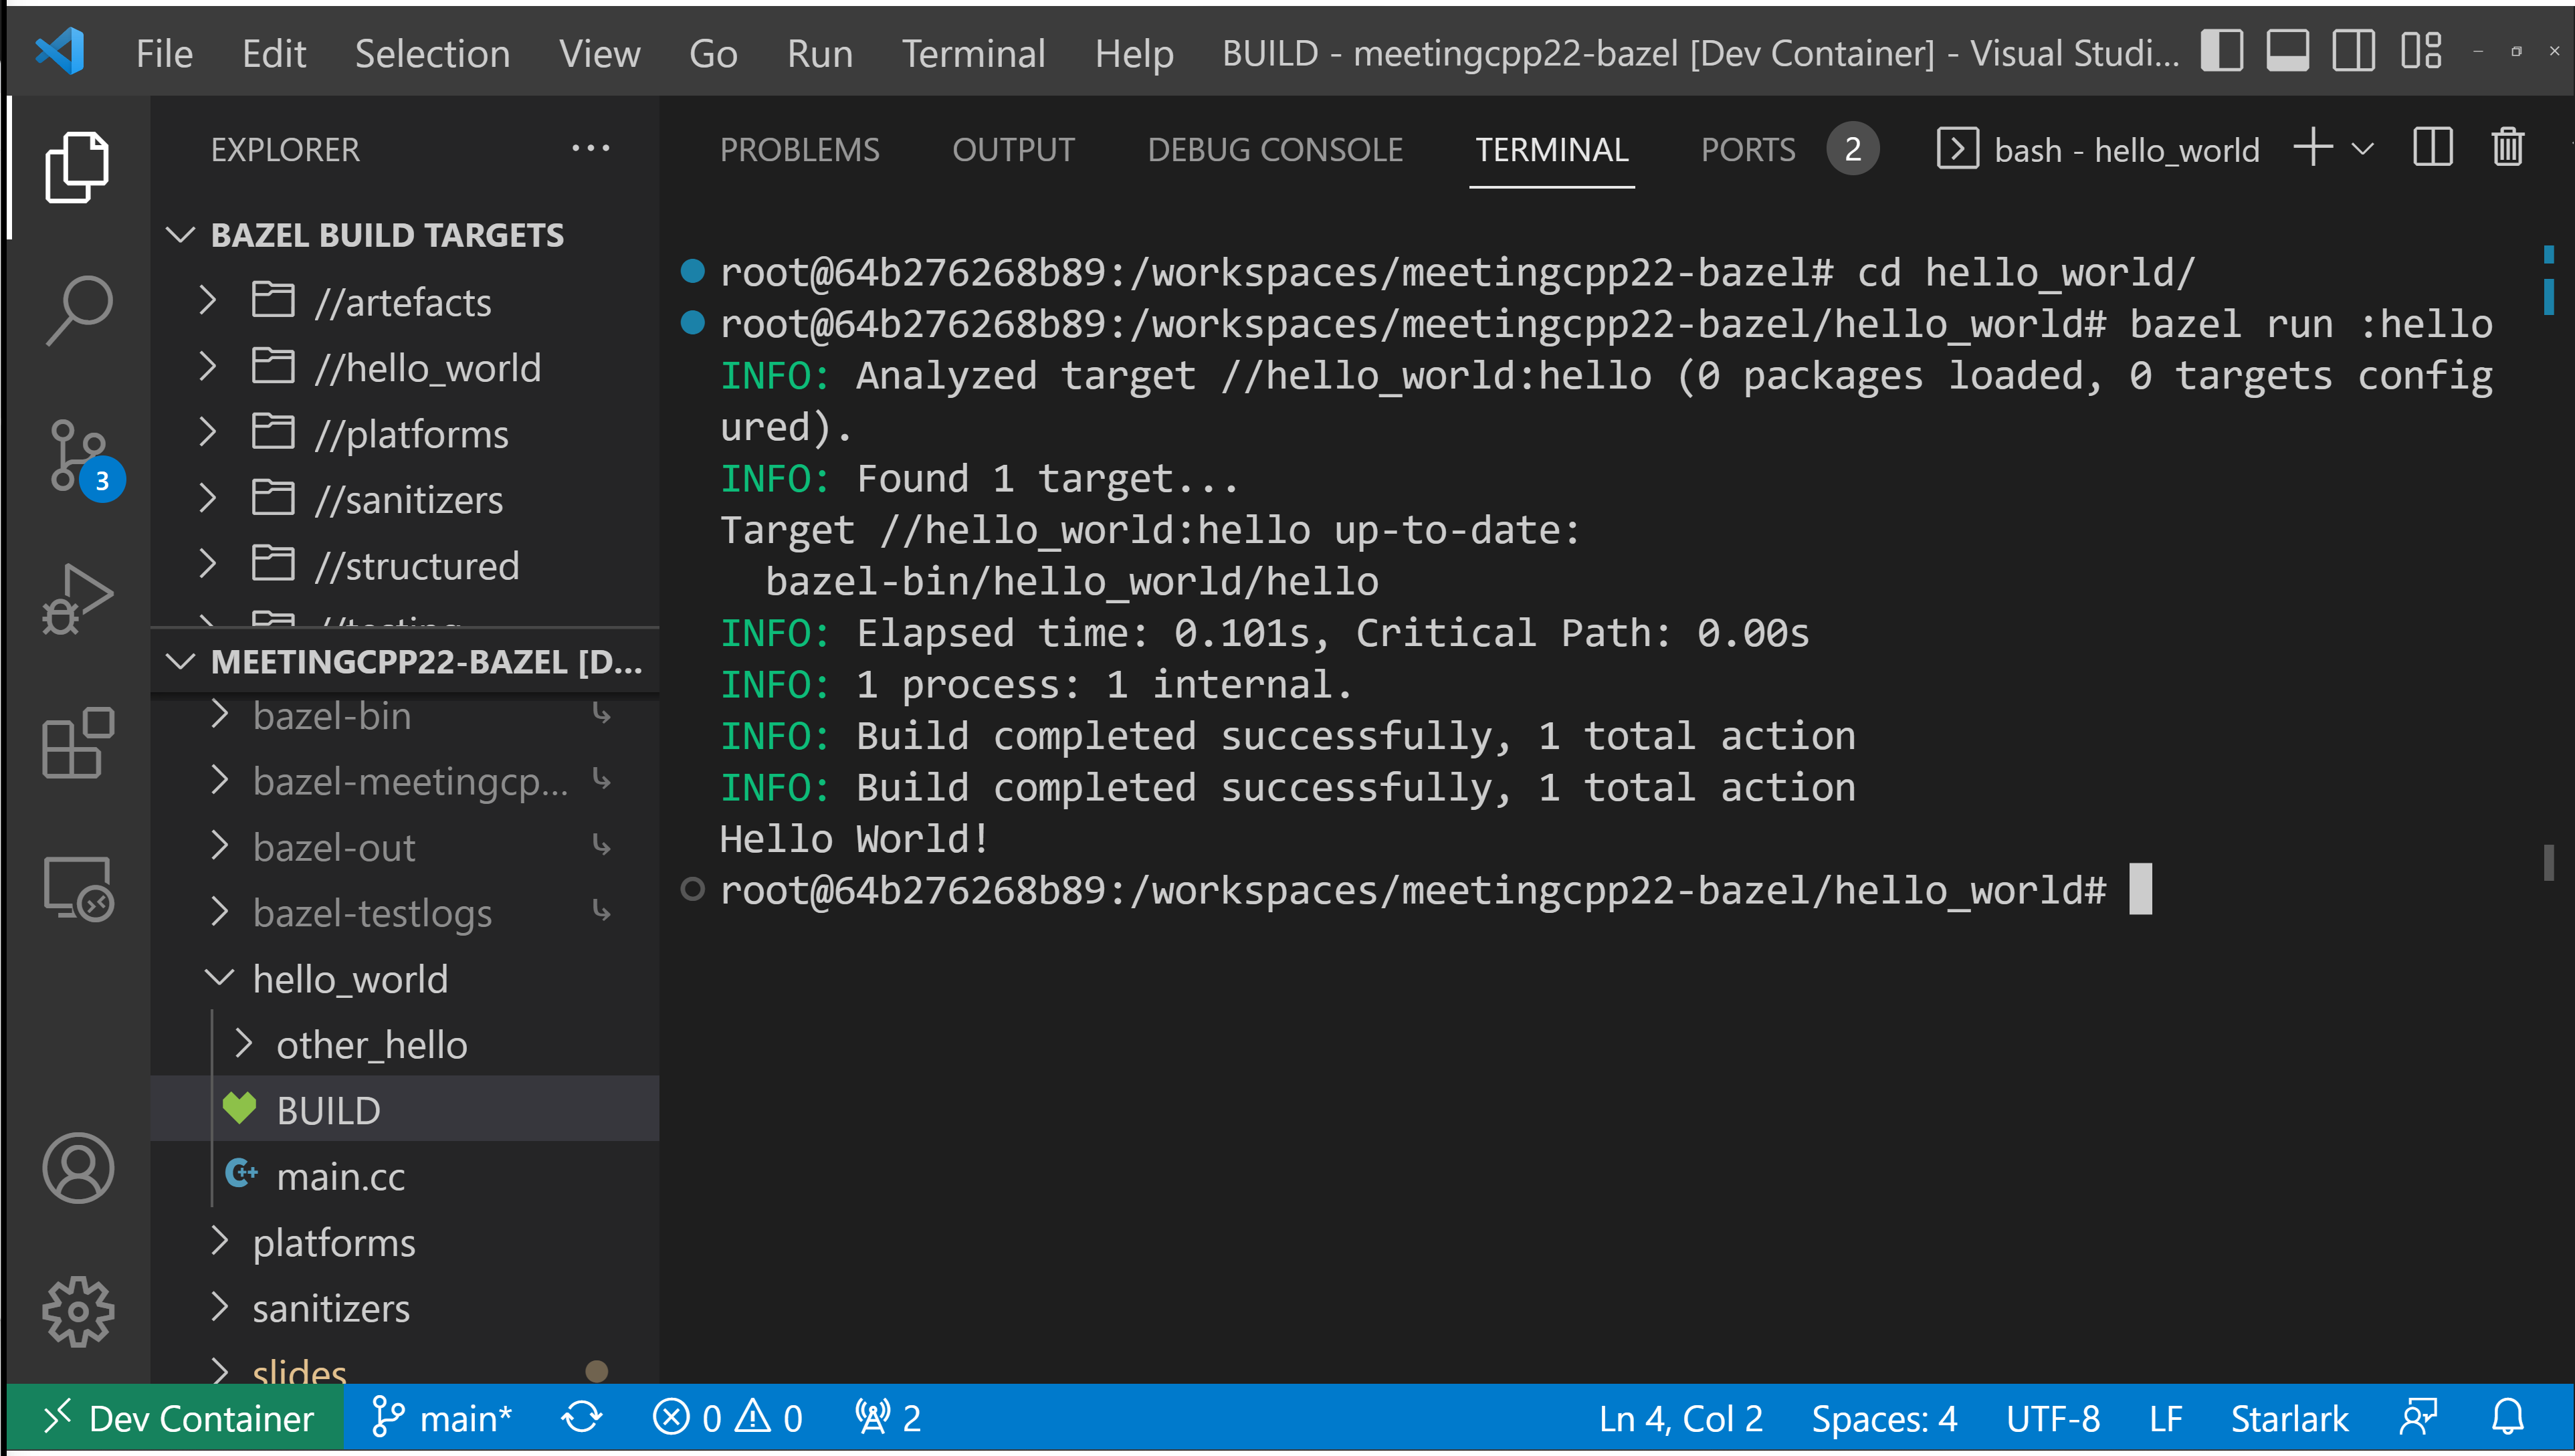
\includegraphics[width=\paperwidth]{slides/static_demos/00_09_local.png}}
\begin{frame}[plain]
\end{frame}
}

{
\usebackgroundtemplate{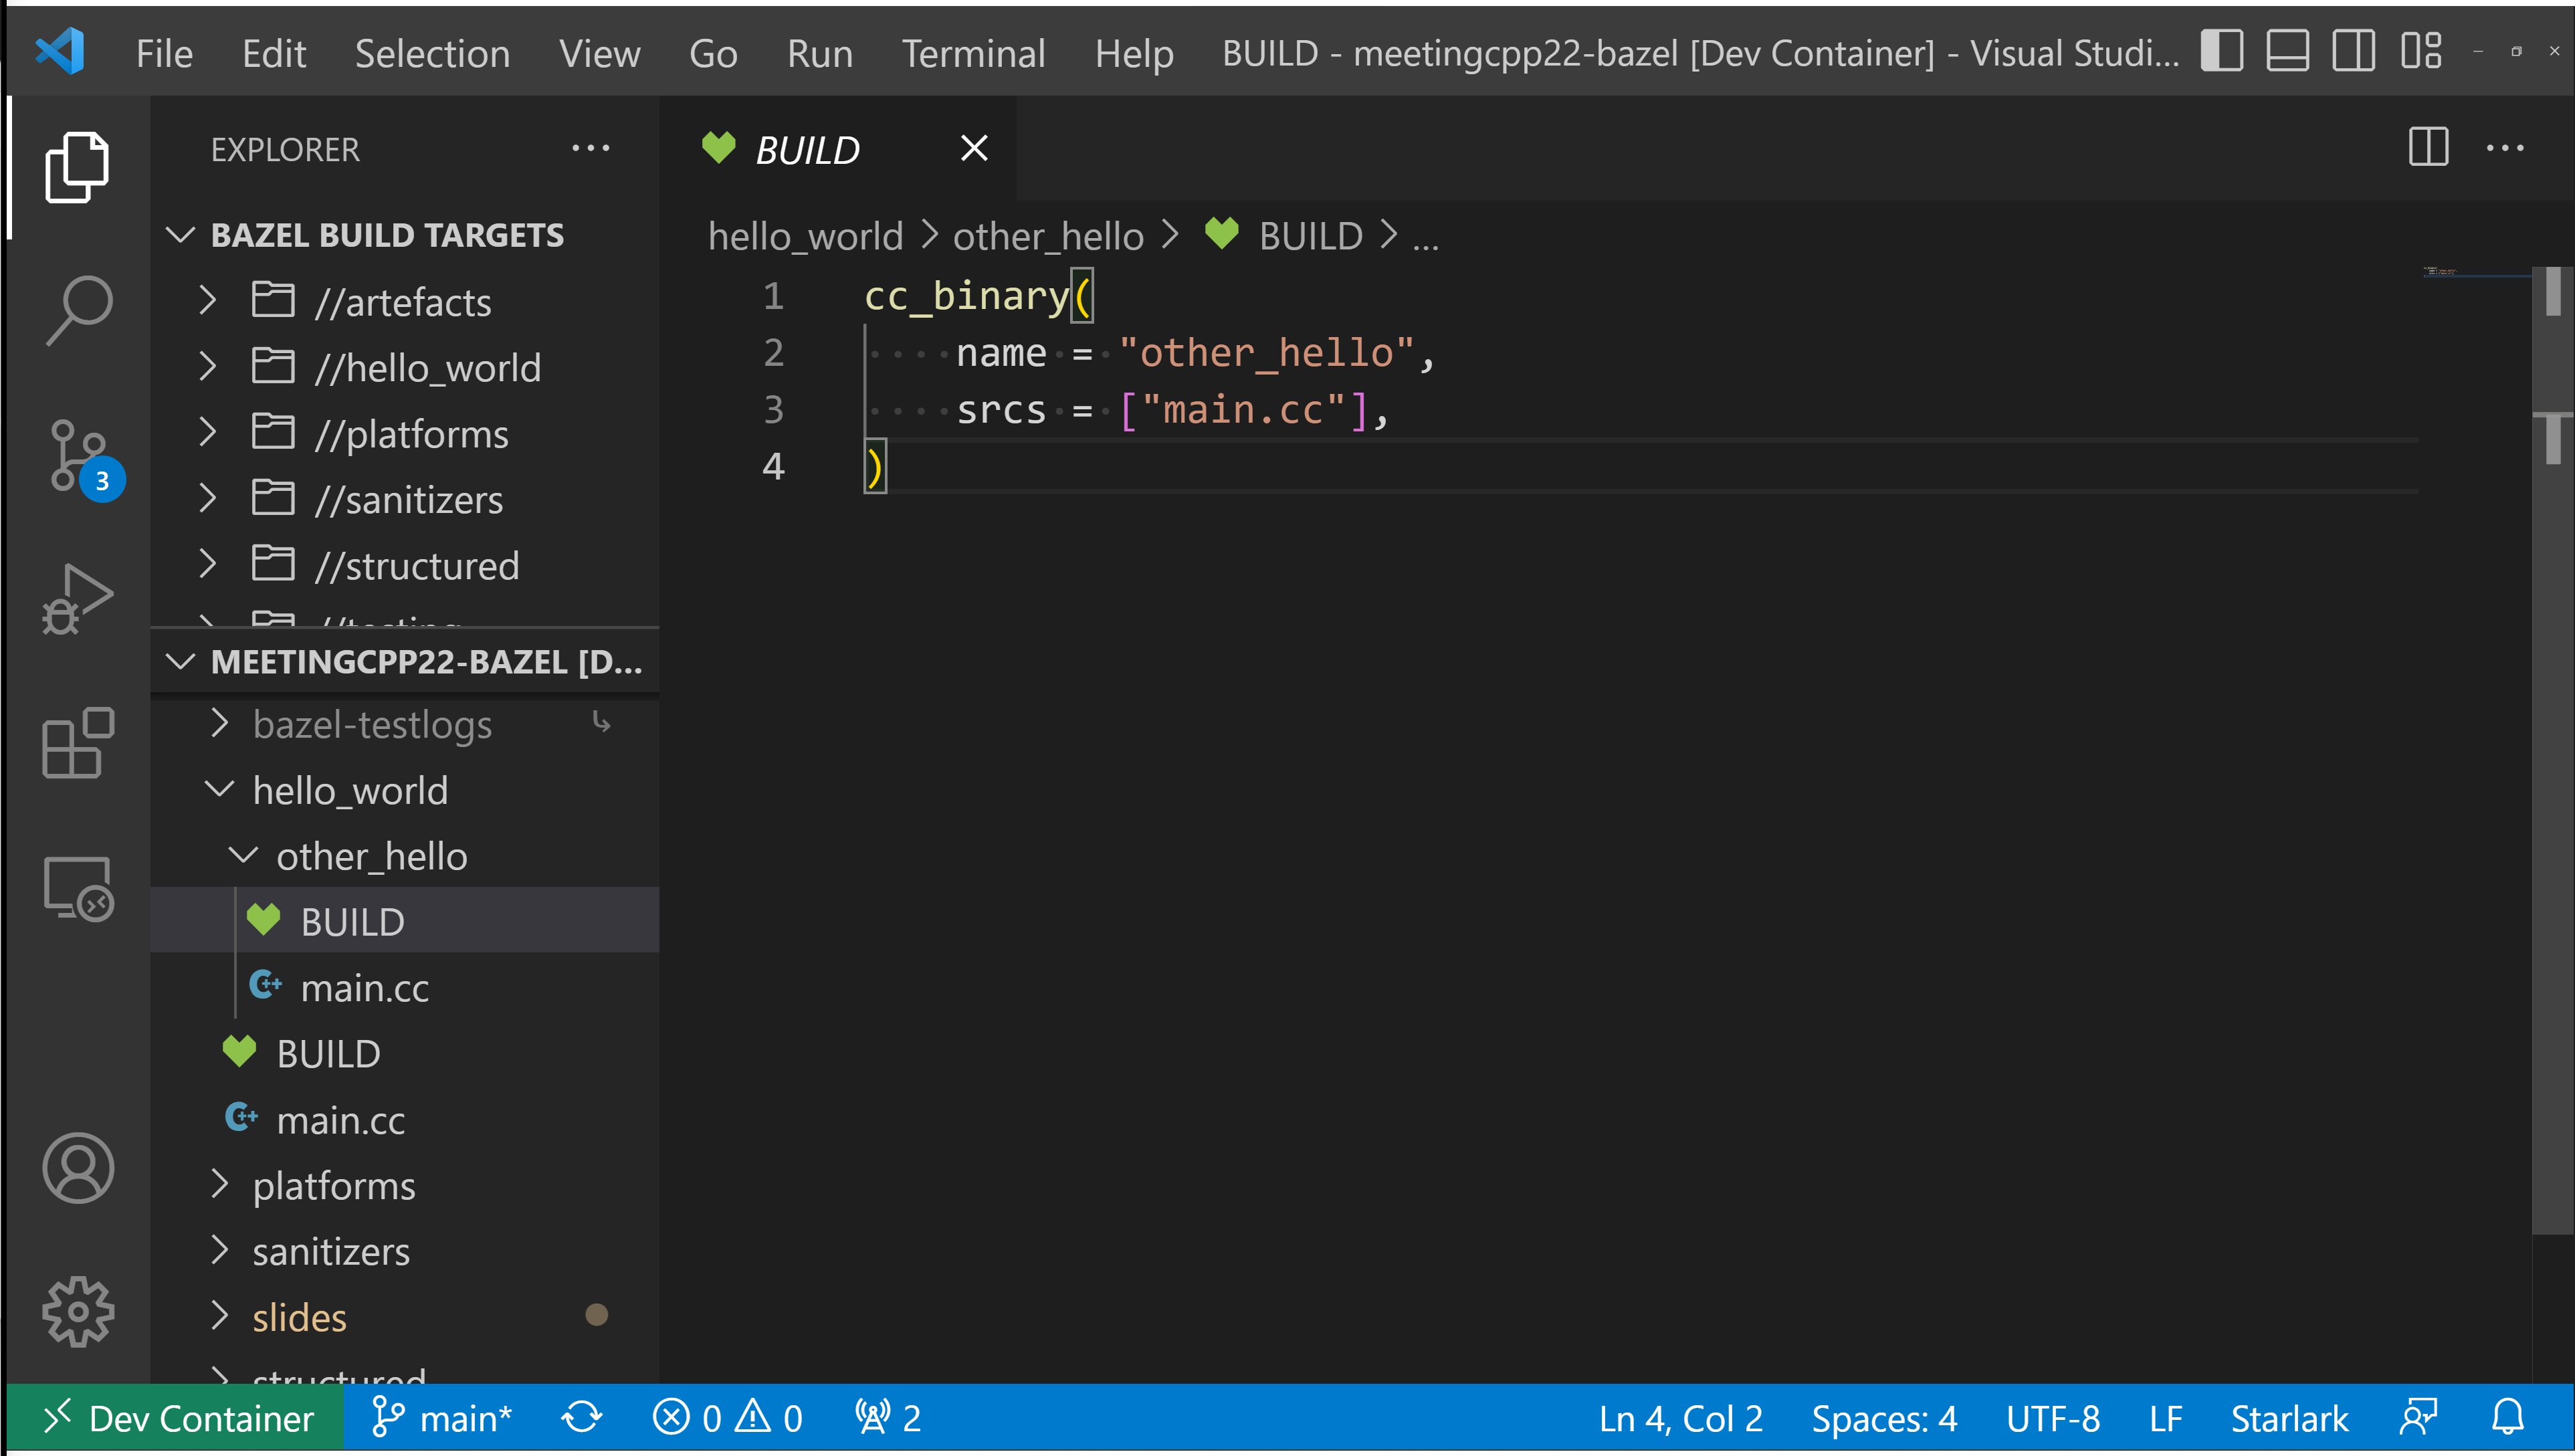
\includegraphics[width=\paperwidth]{slides/static_demos/00_10_other_hello.png}}
\begin{frame}[plain]
\end{frame}
}

{
\usebackgroundtemplate{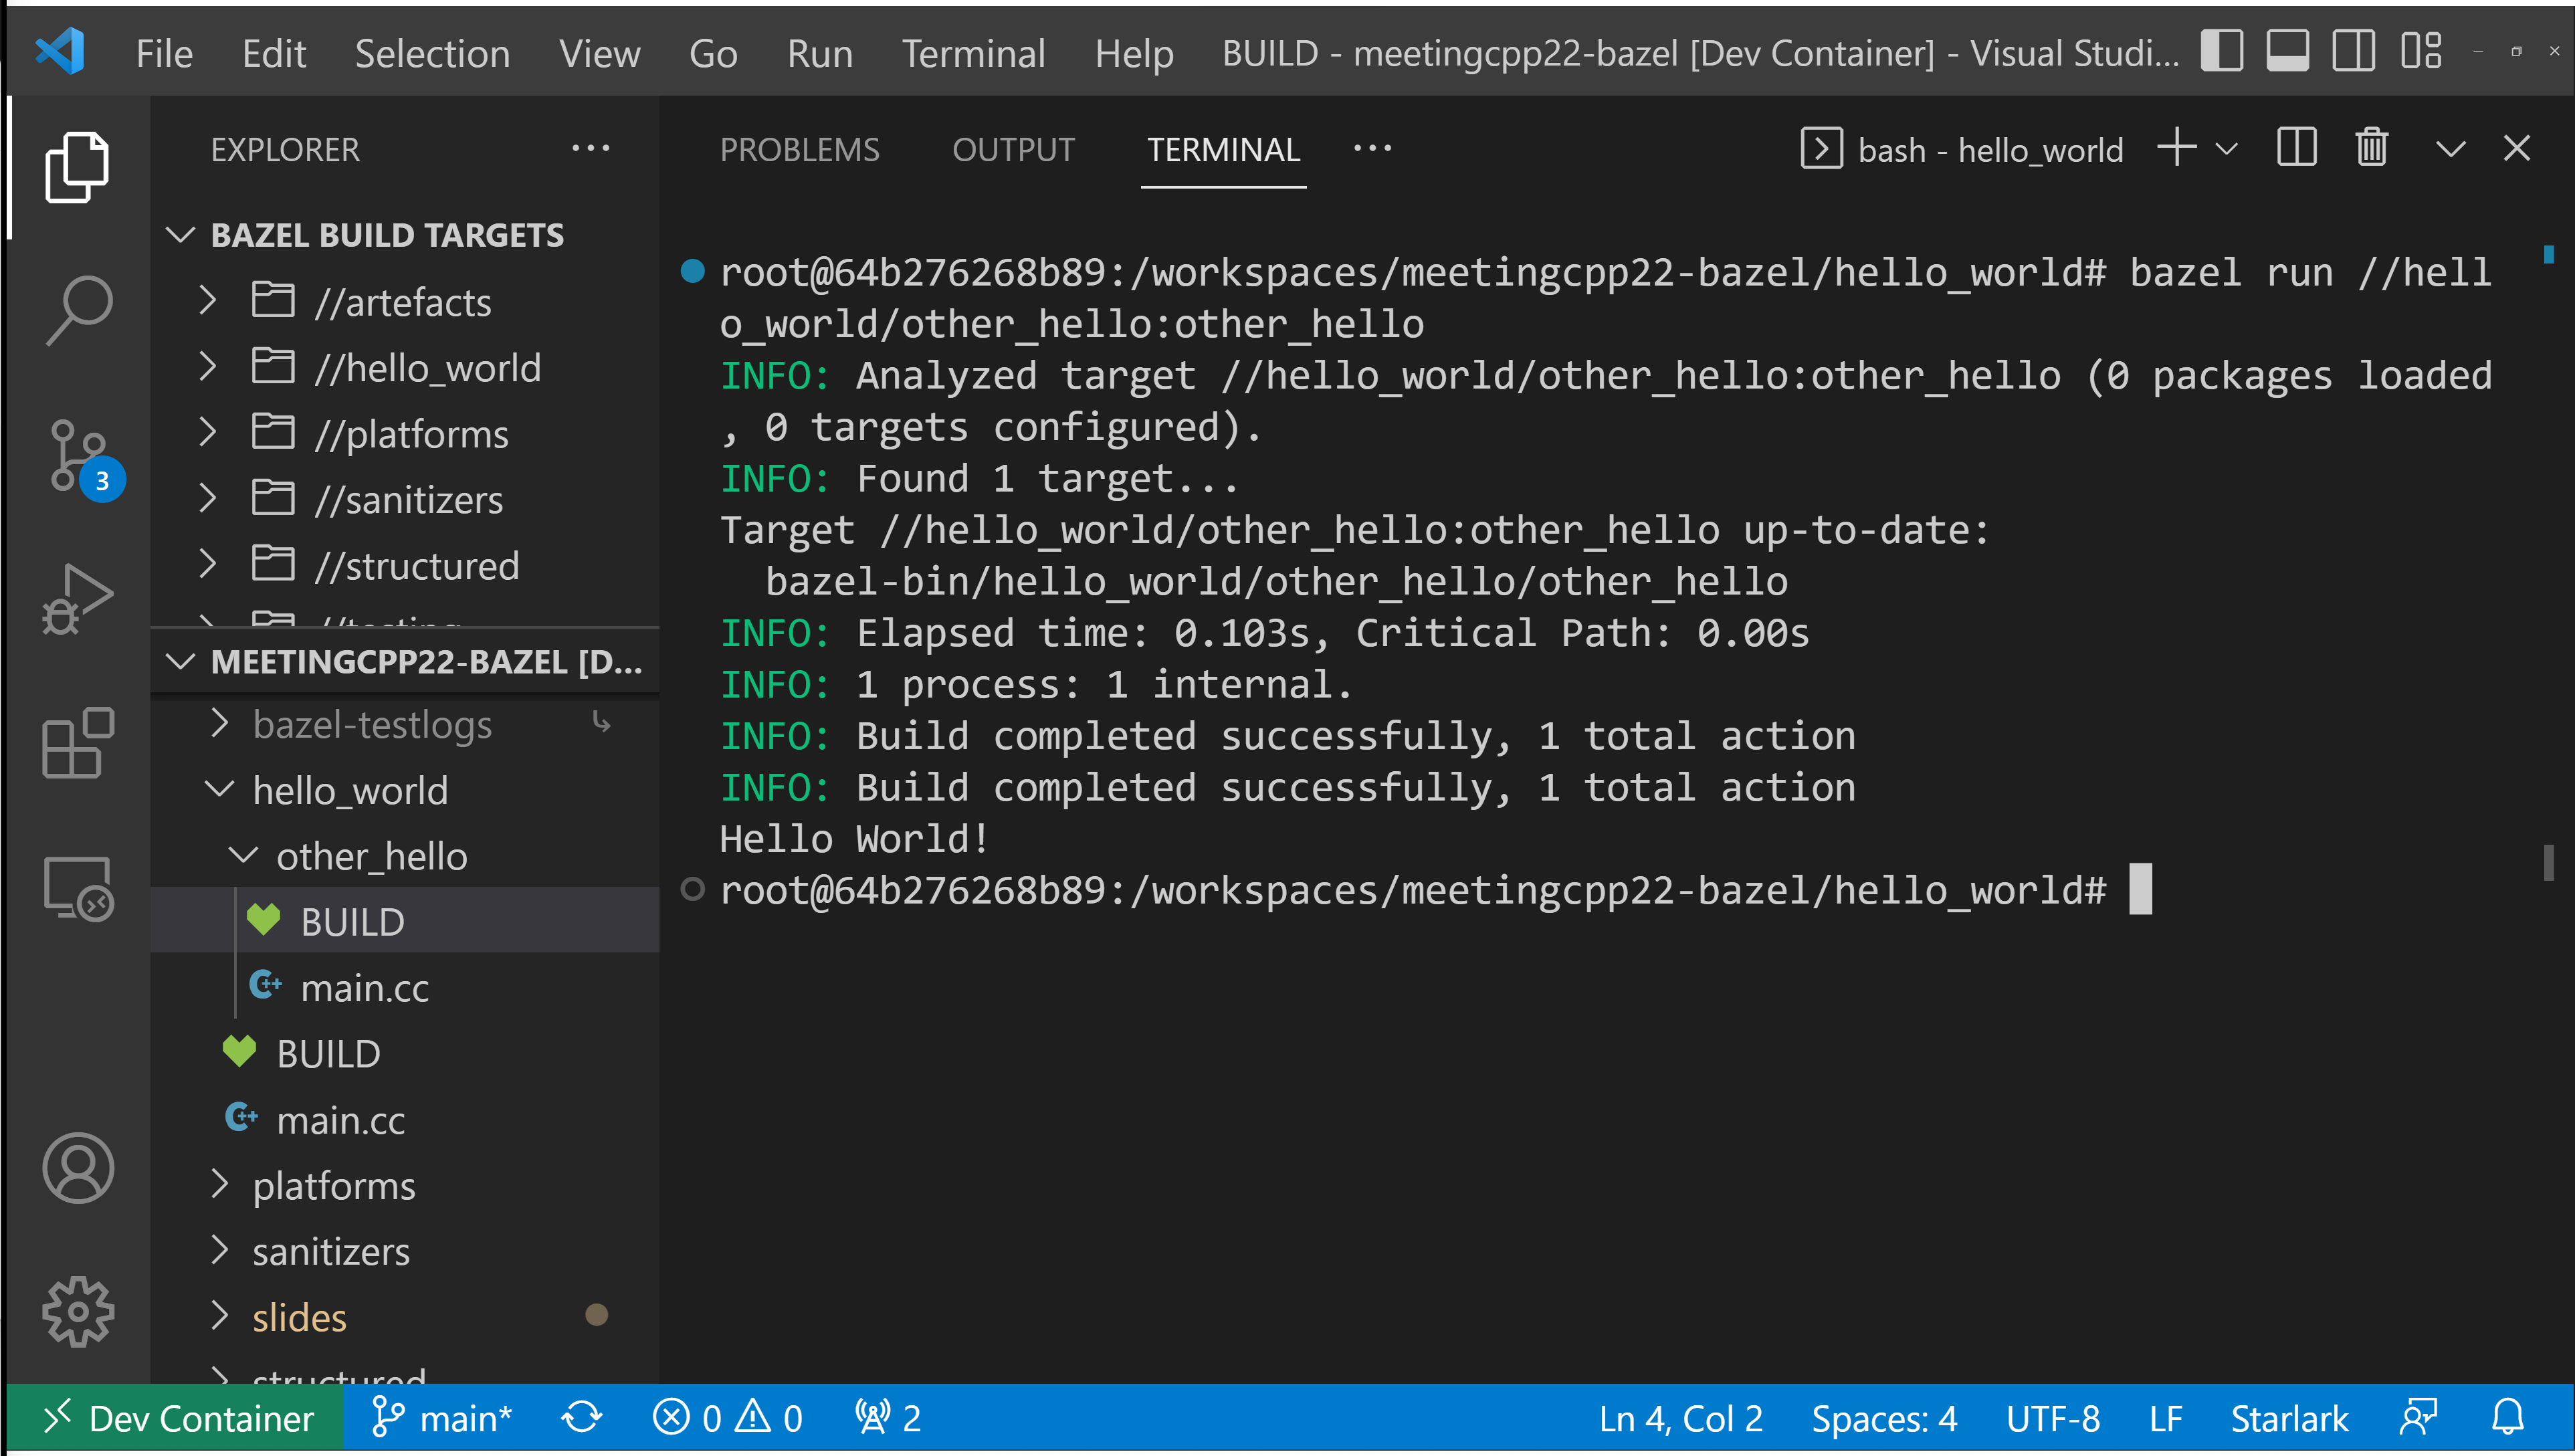
\includegraphics[width=\paperwidth]{slides/static_demos/00_11_other_run.png}}
\begin{frame}[plain]
\end{frame}
}

{
\usebackgroundtemplate{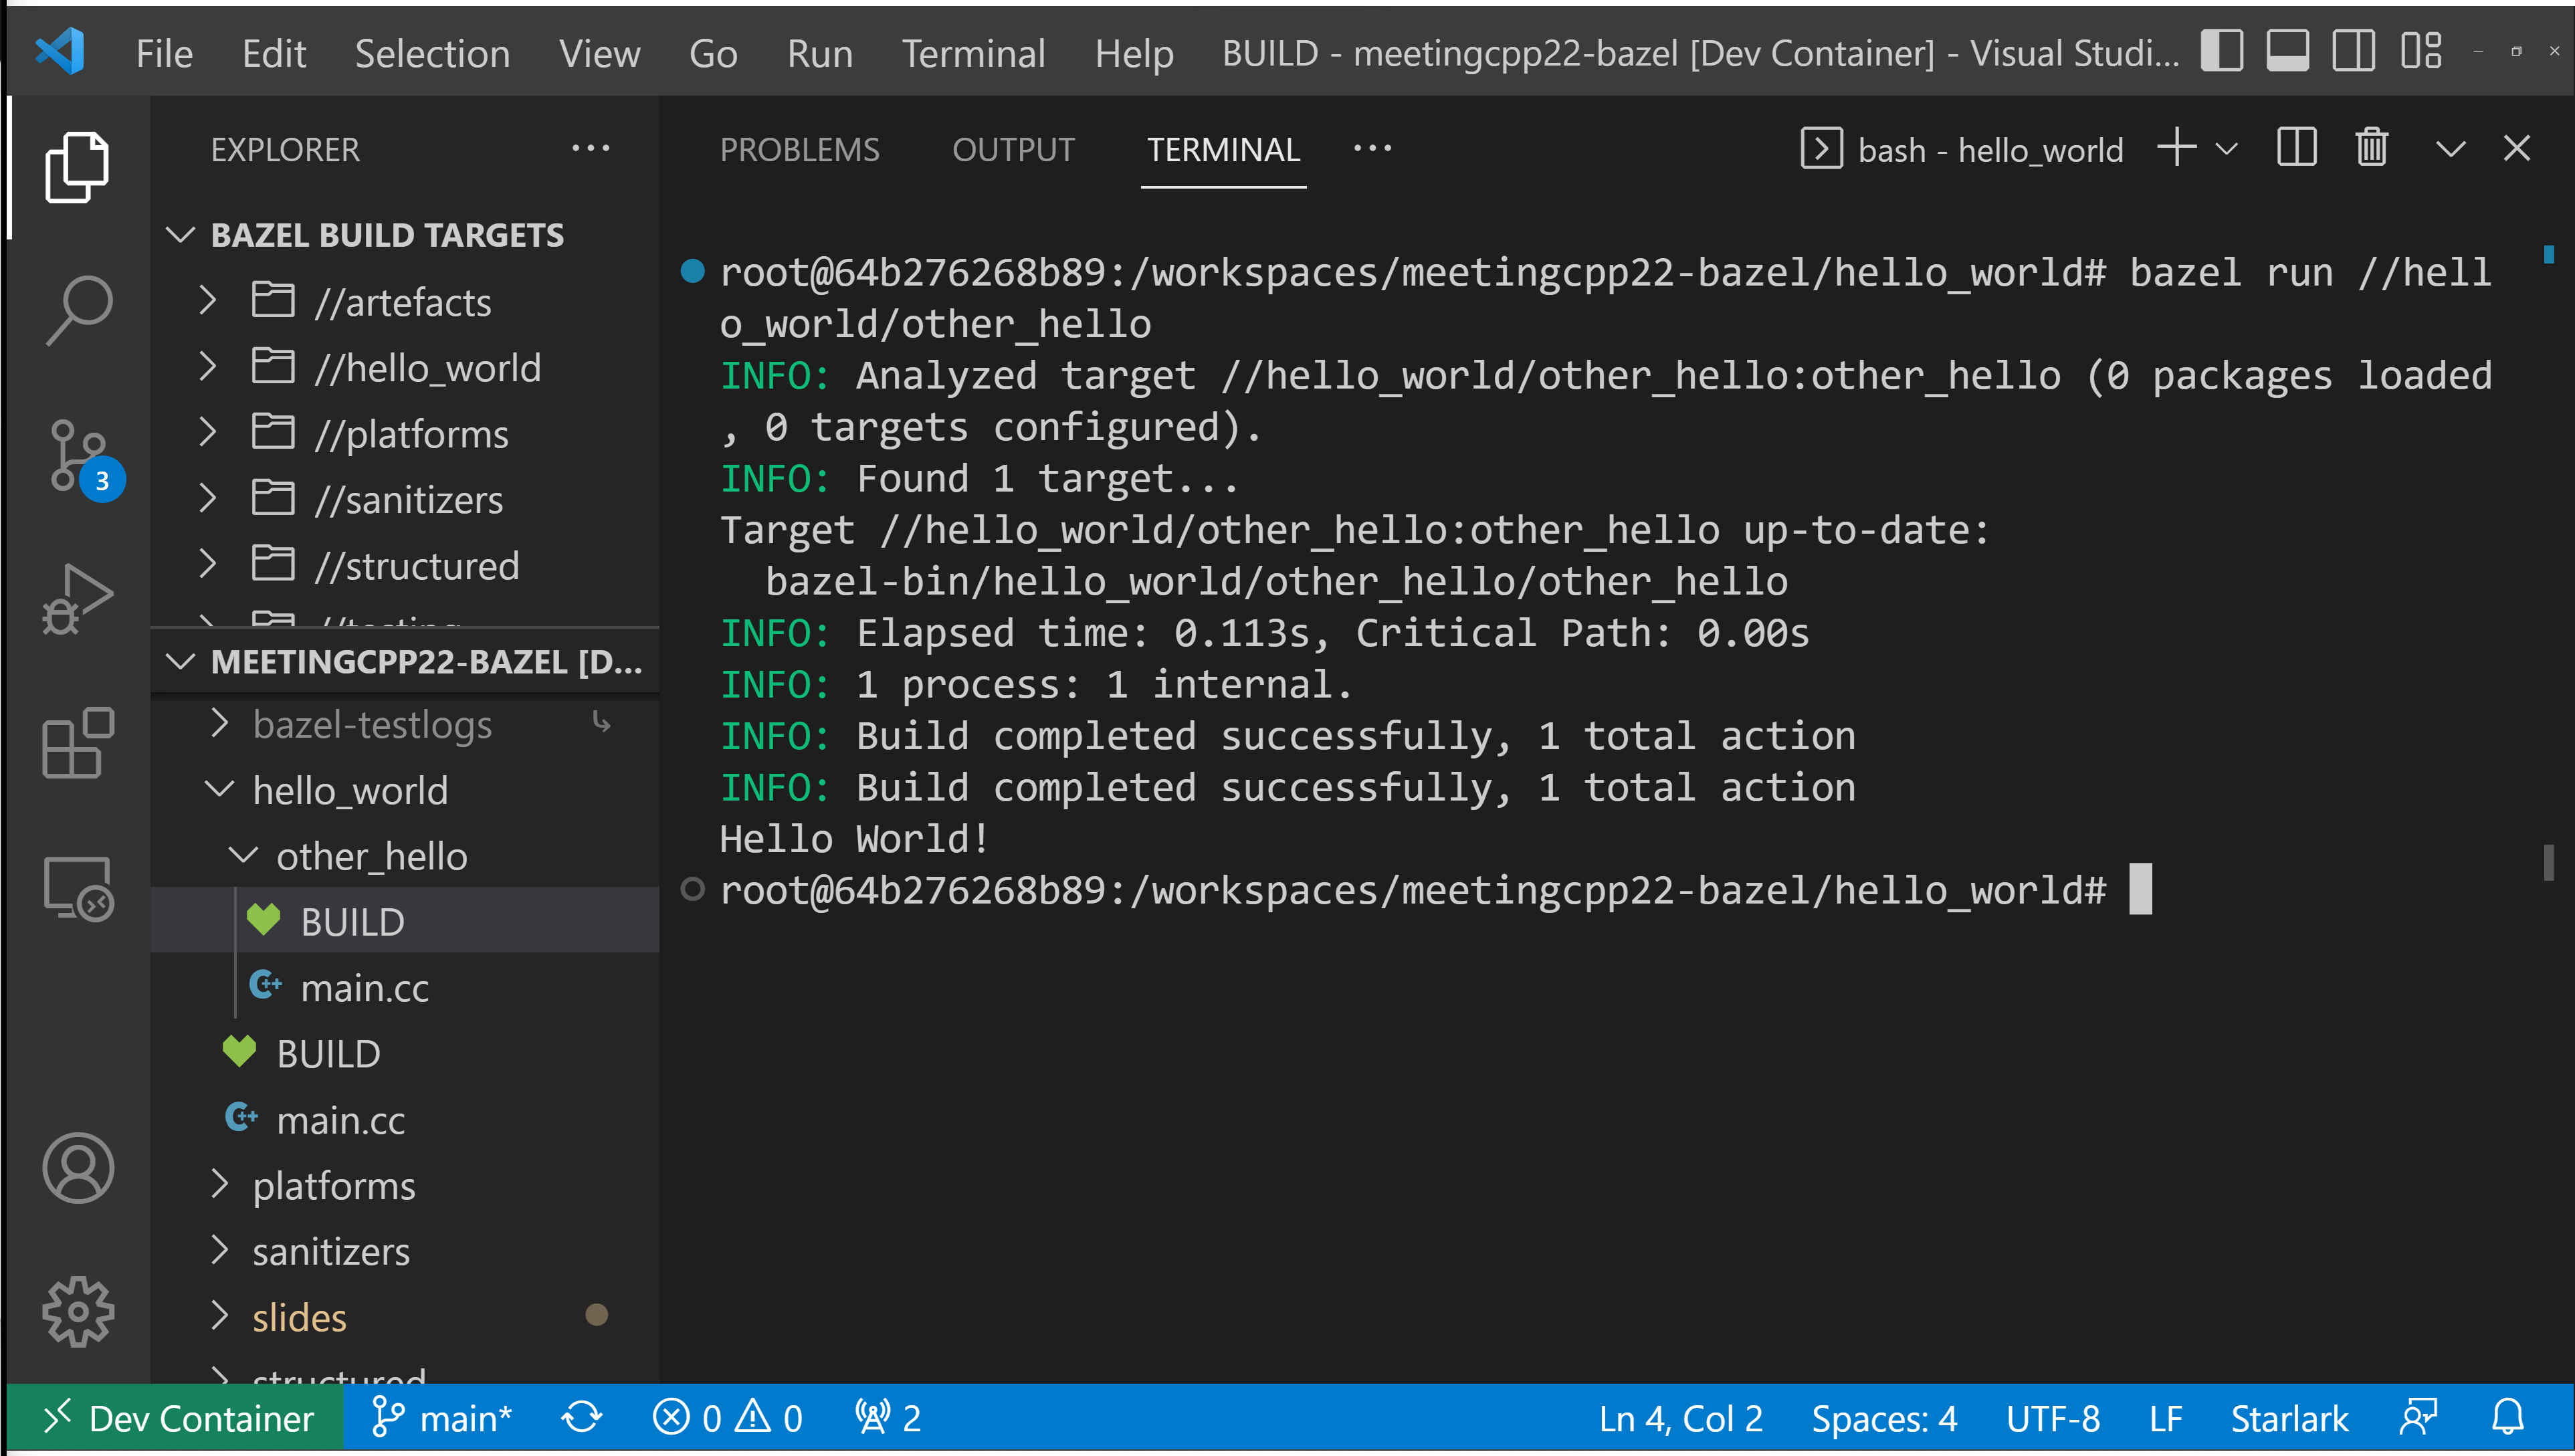
\includegraphics[width=\paperwidth]{slides/static_demos/00_12_other_run_short.png}}
\begin{frame}[plain]
\end{frame}
}

\begin{frame}{}
    \begin{center}
        \begin{Huge}Structured Code\end{Huge}
    \end{center}
\end{frame}


{
\usebackgroundtemplate{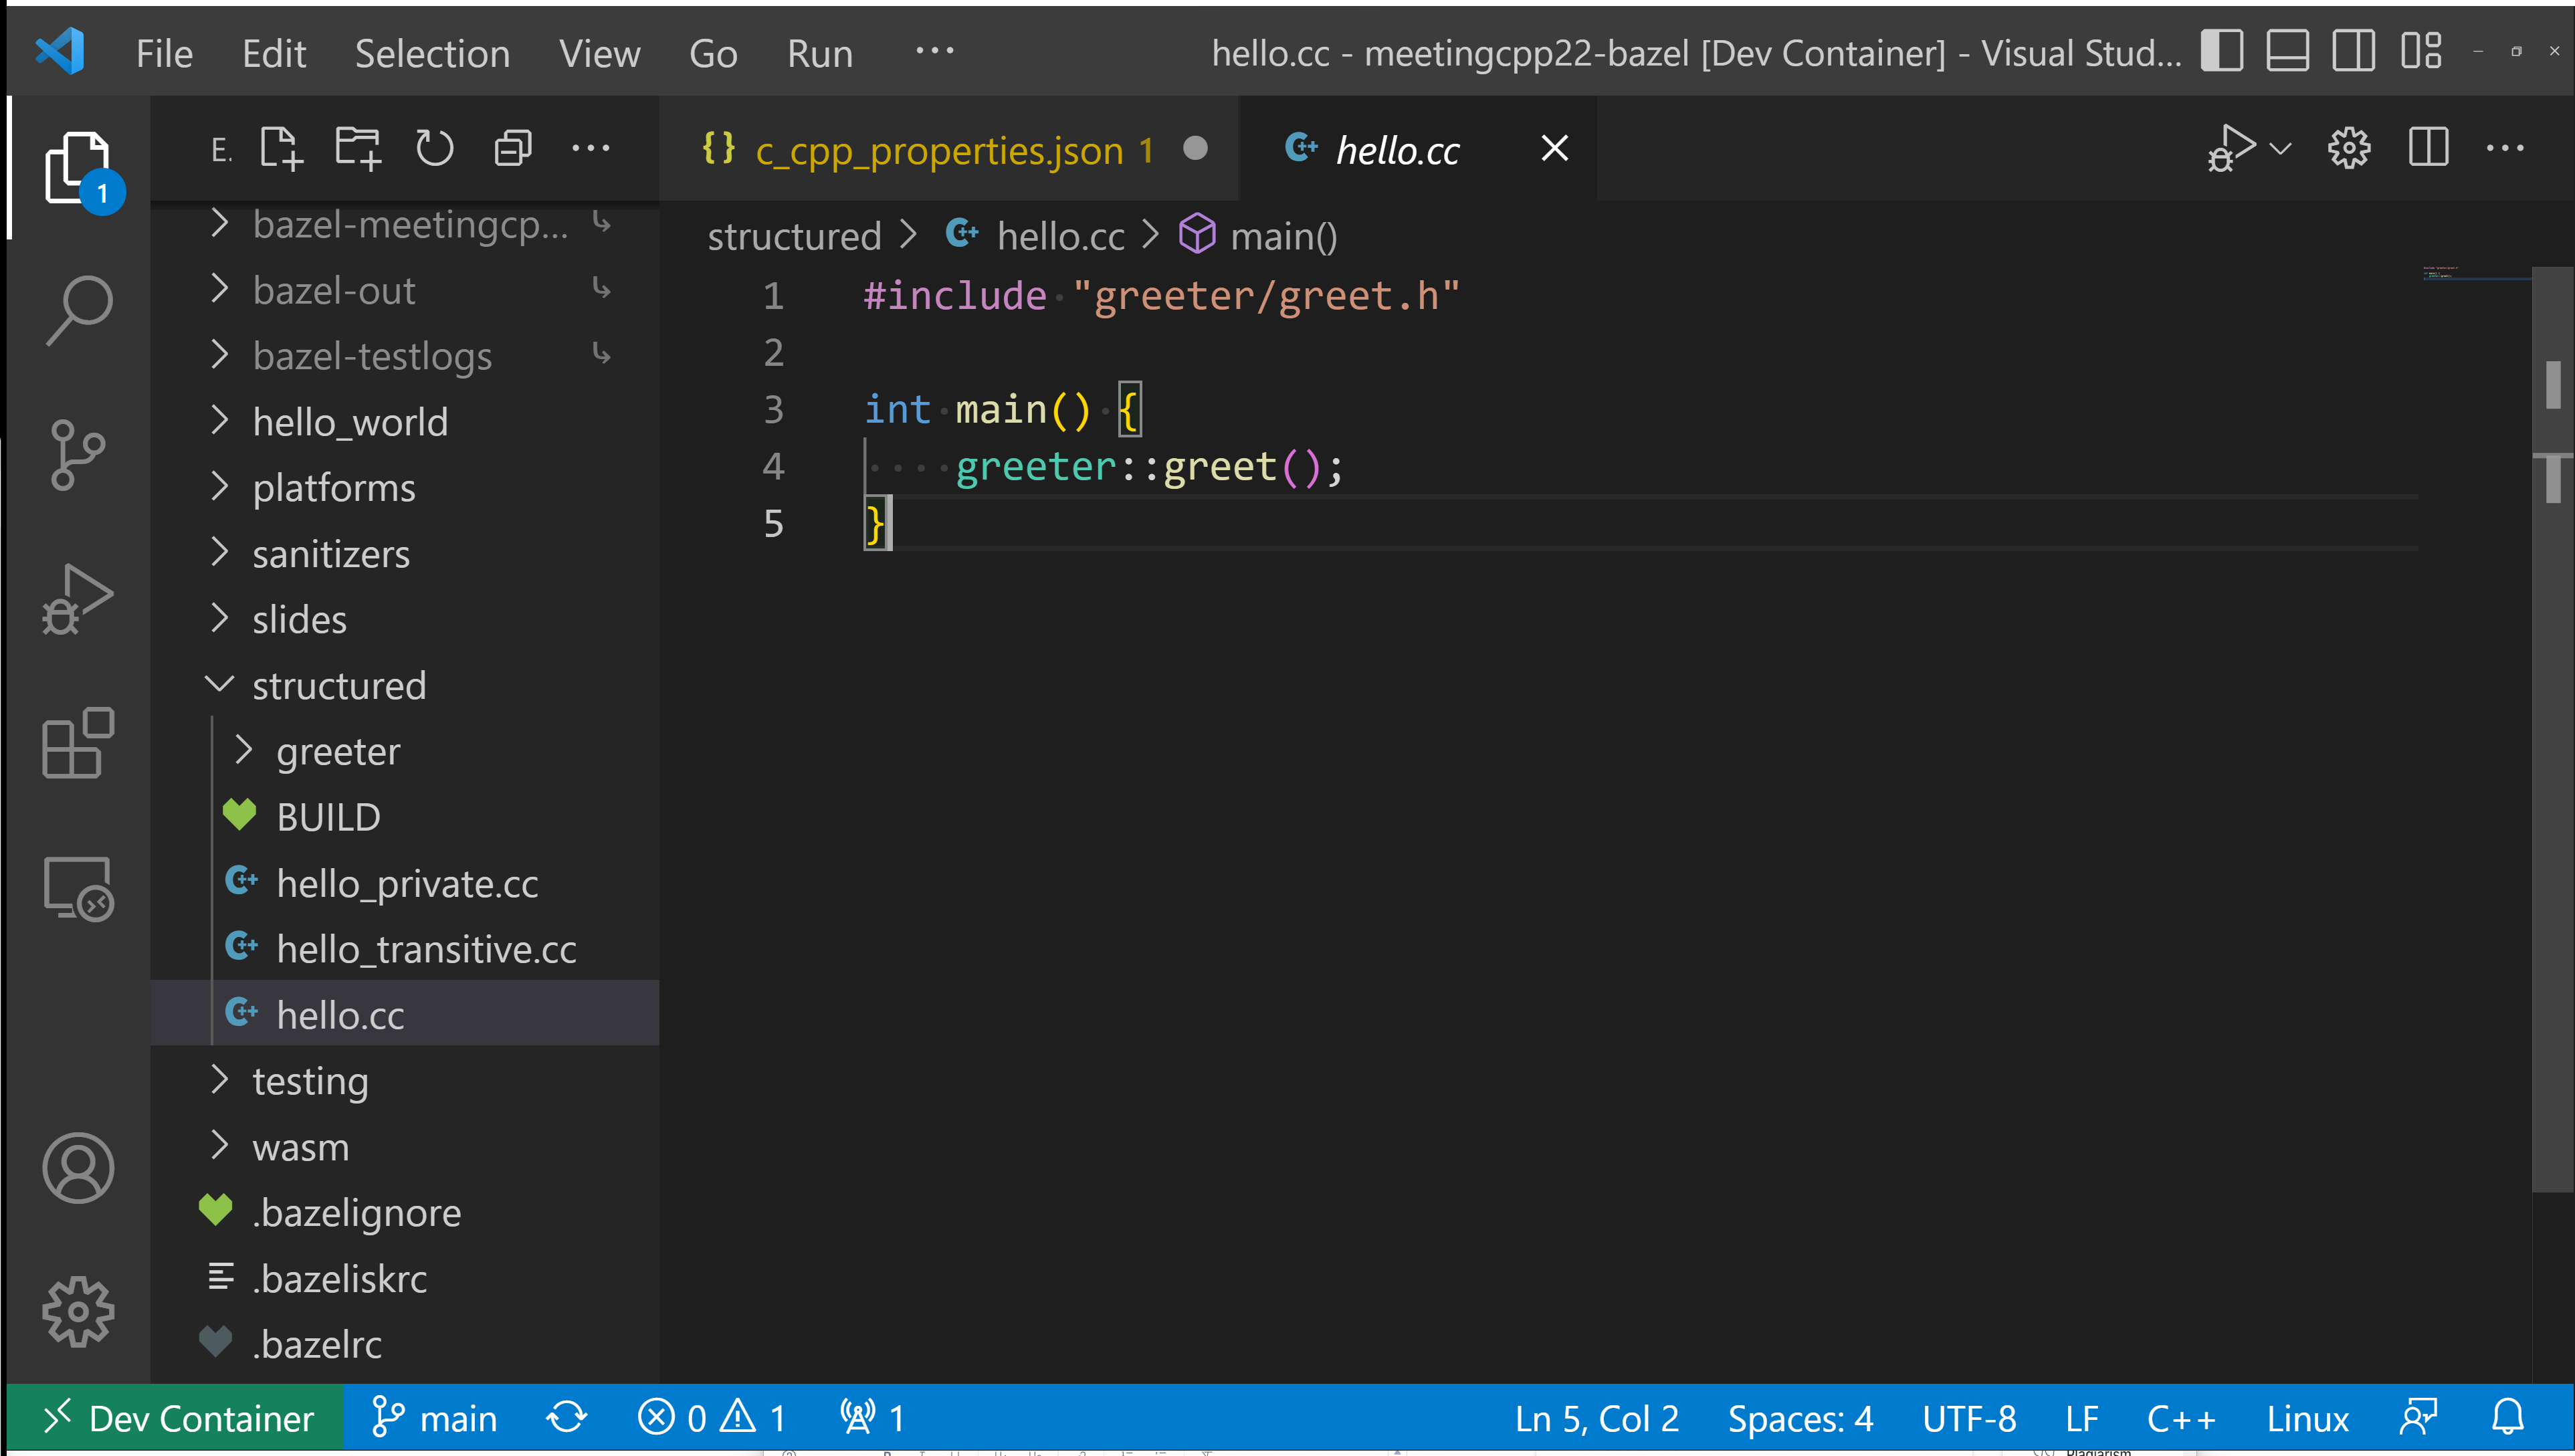
\includegraphics[width=\paperwidth]{slides/static_demos/01_00_main.png}}
\begin{frame}[plain]
\end{frame}
}

{
\usebackgroundtemplate{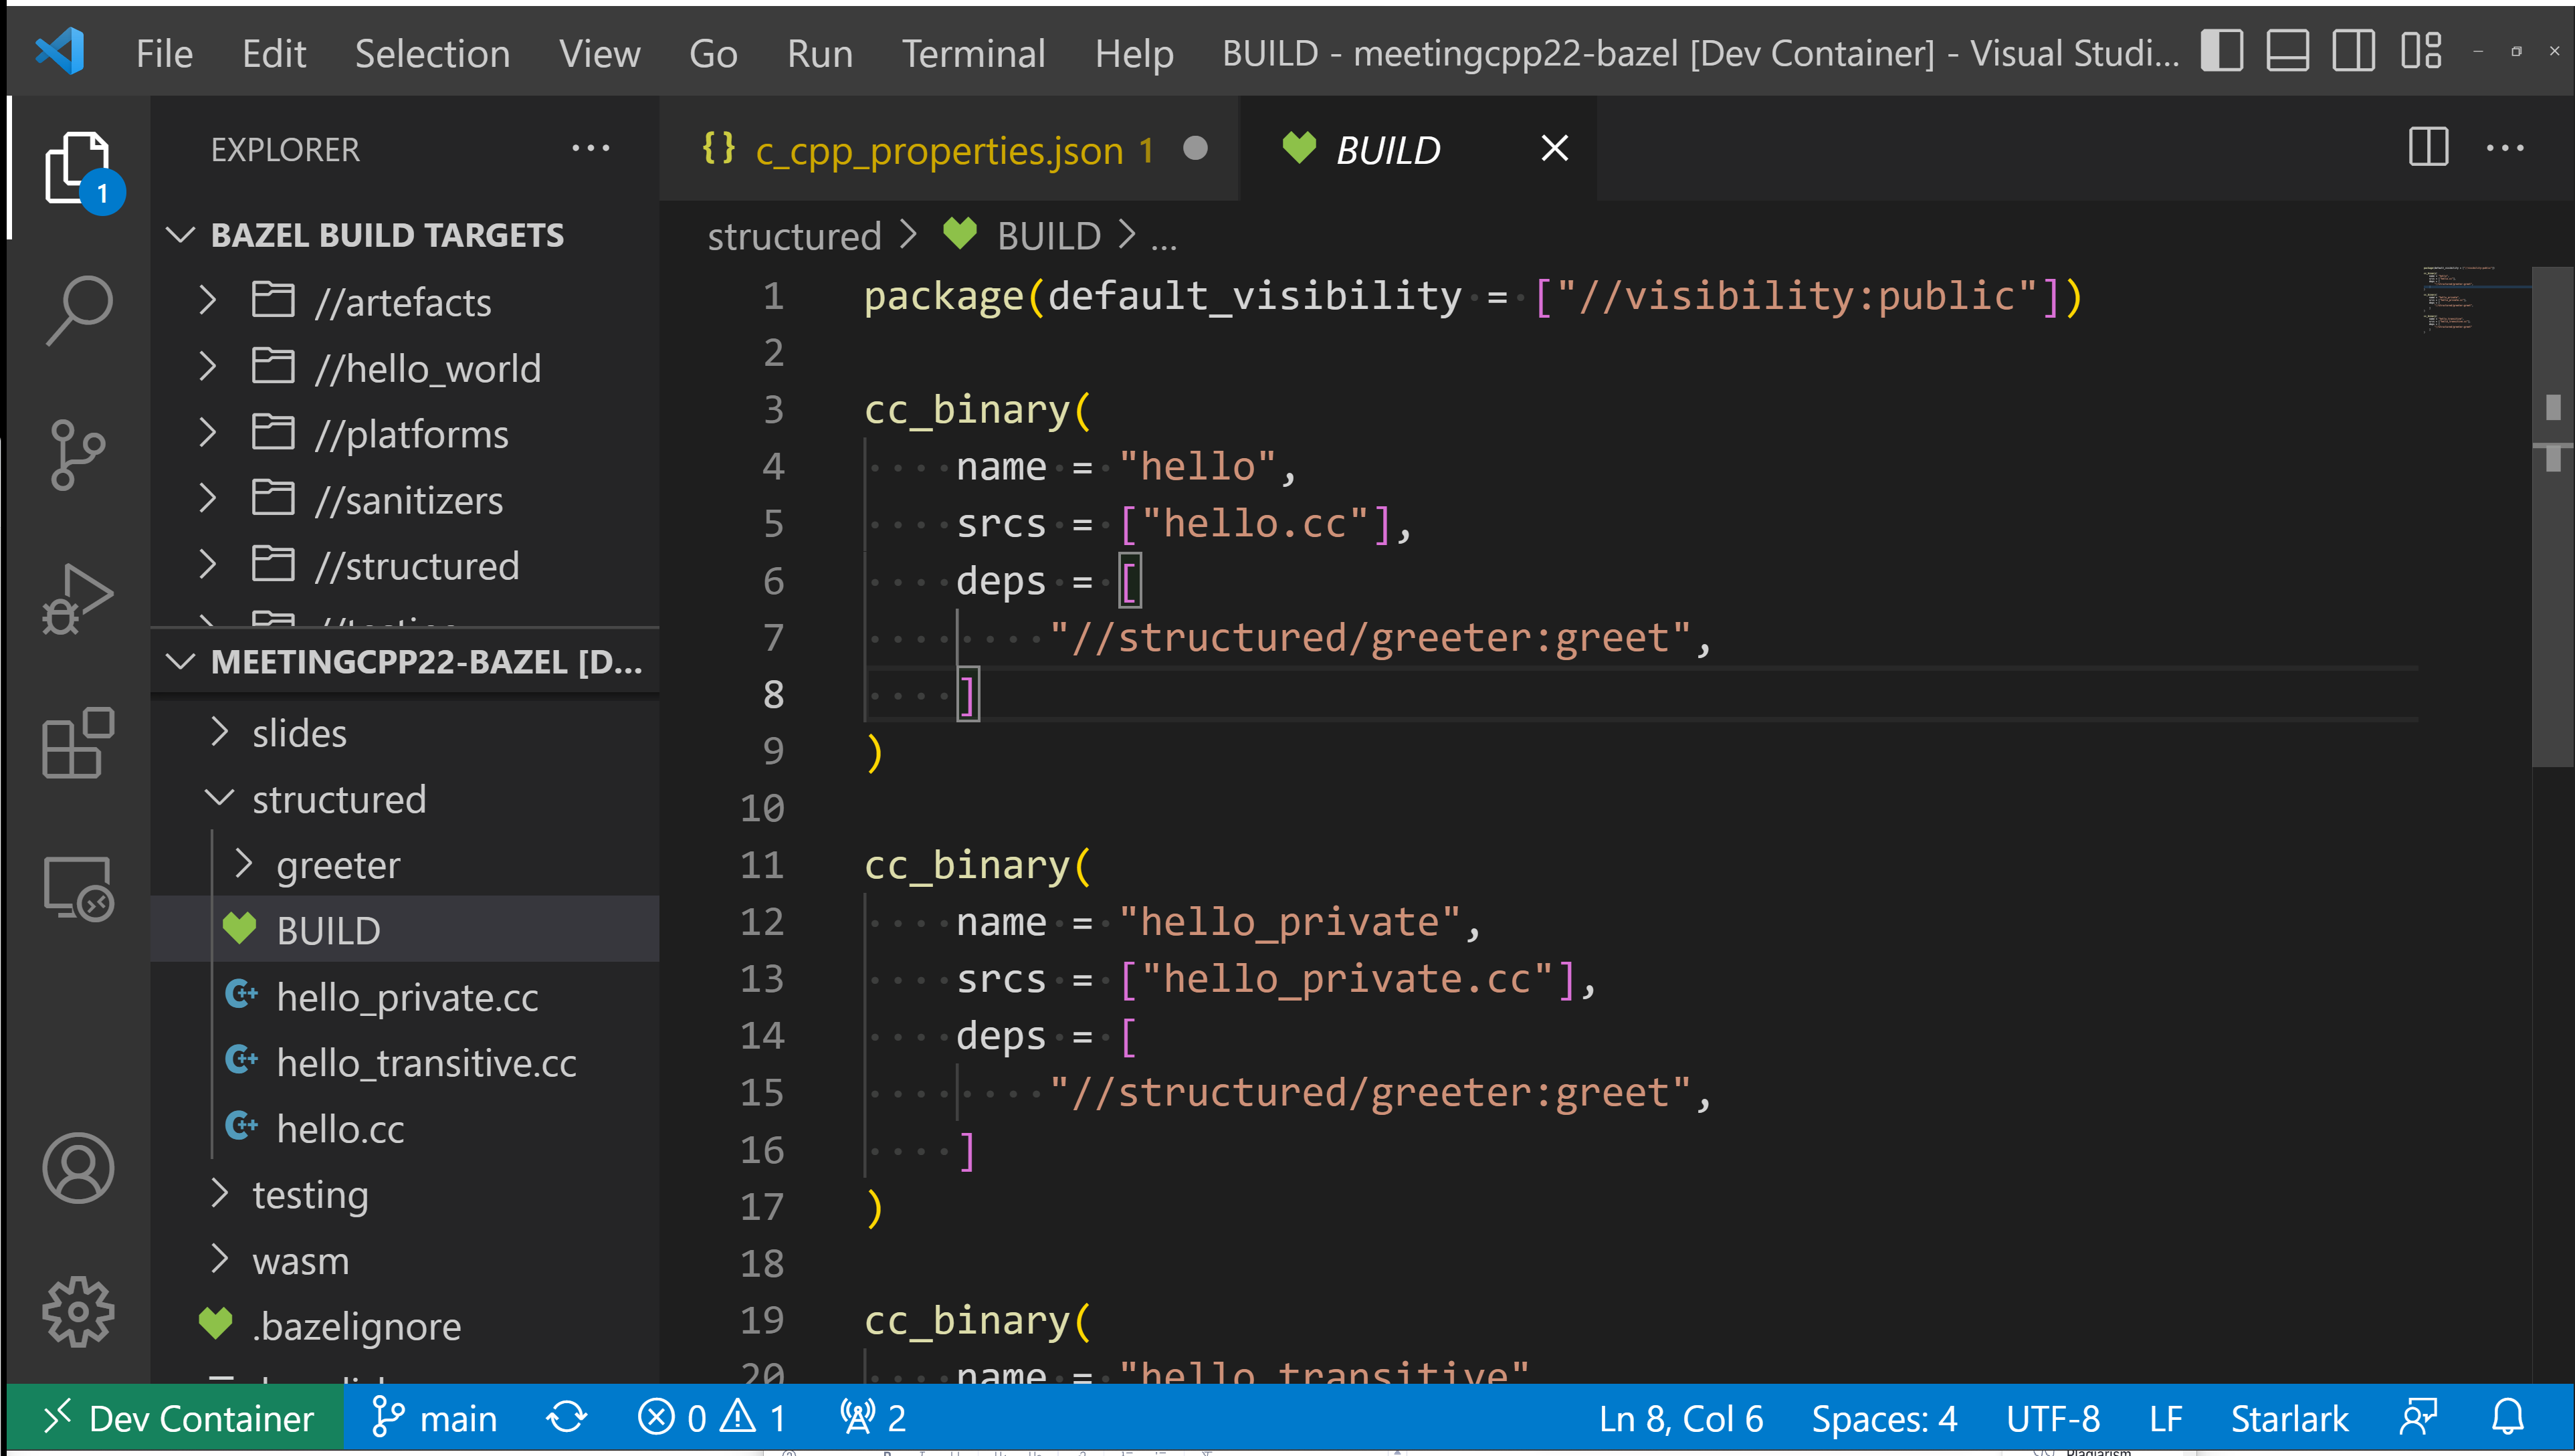
\includegraphics[width=\paperwidth]{slides/static_demos/01_01_BUILD.png}}
\begin{frame}[plain]
\end{frame}
}

{
\usebackgroundtemplate{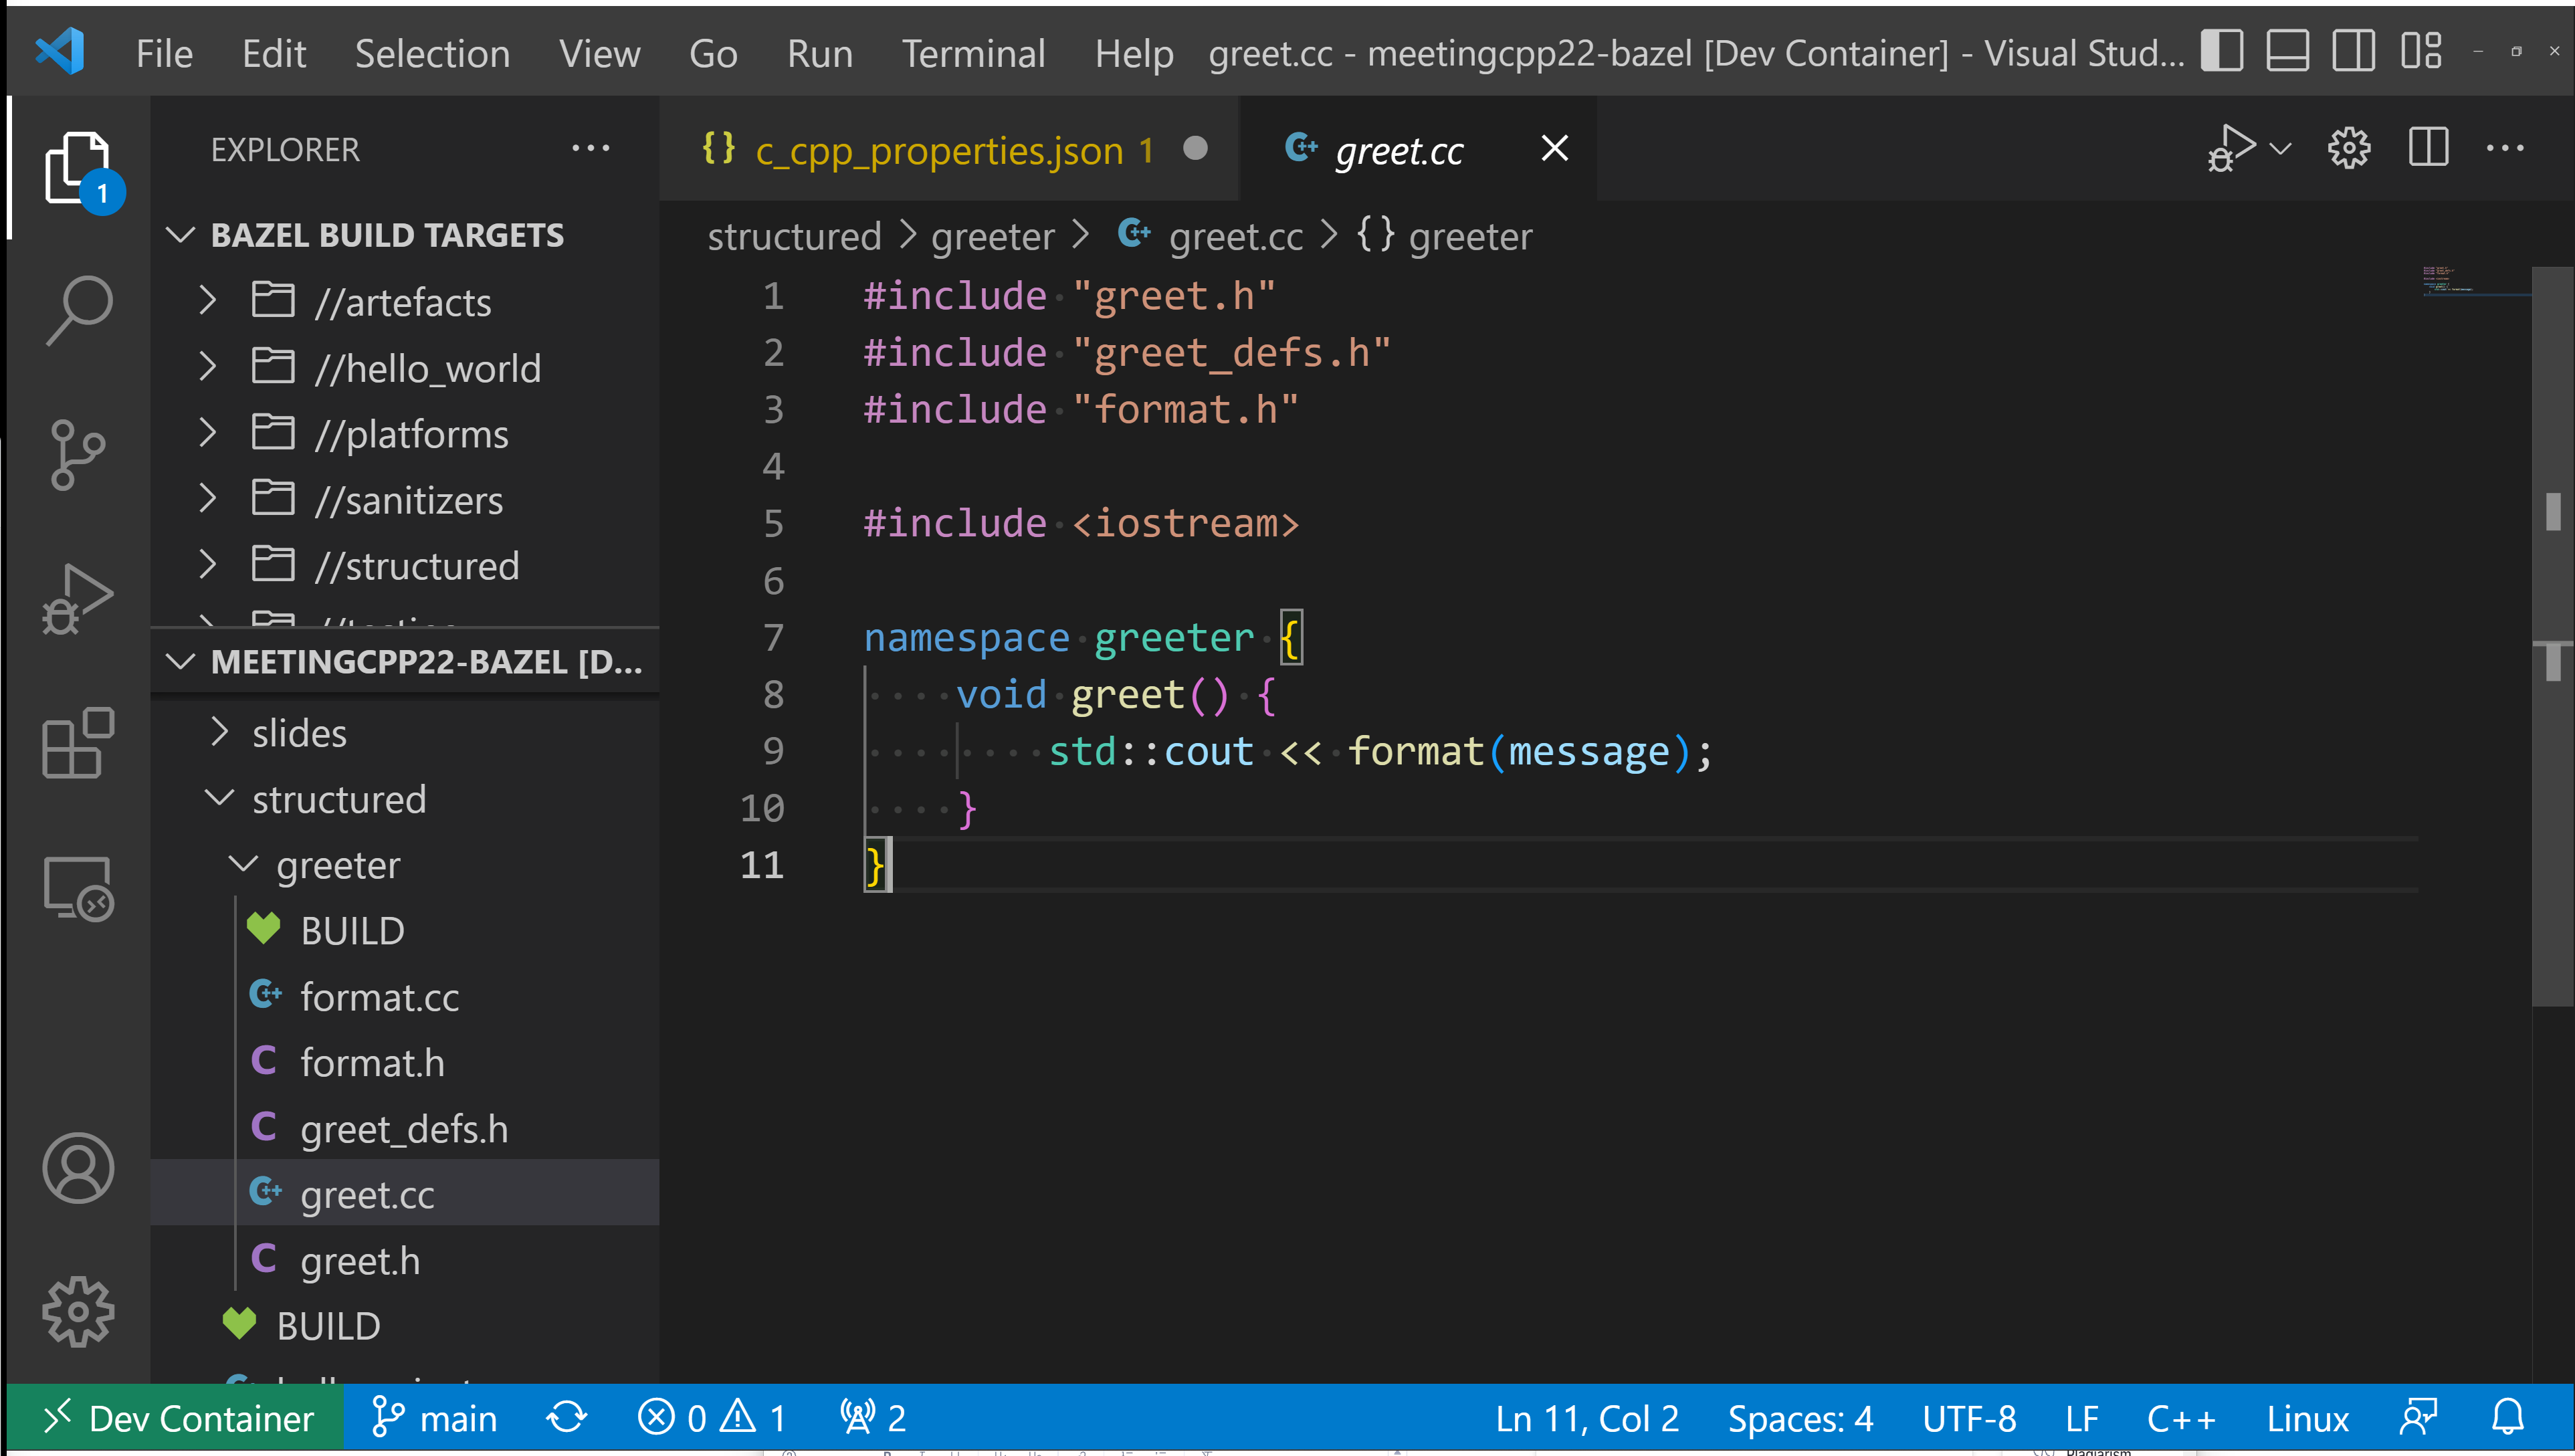
\includegraphics[width=\paperwidth]{slides/static_demos/01_02_greeter.png}}
\begin{frame}[plain]
\end{frame}
}



{
\usebackgroundtemplate{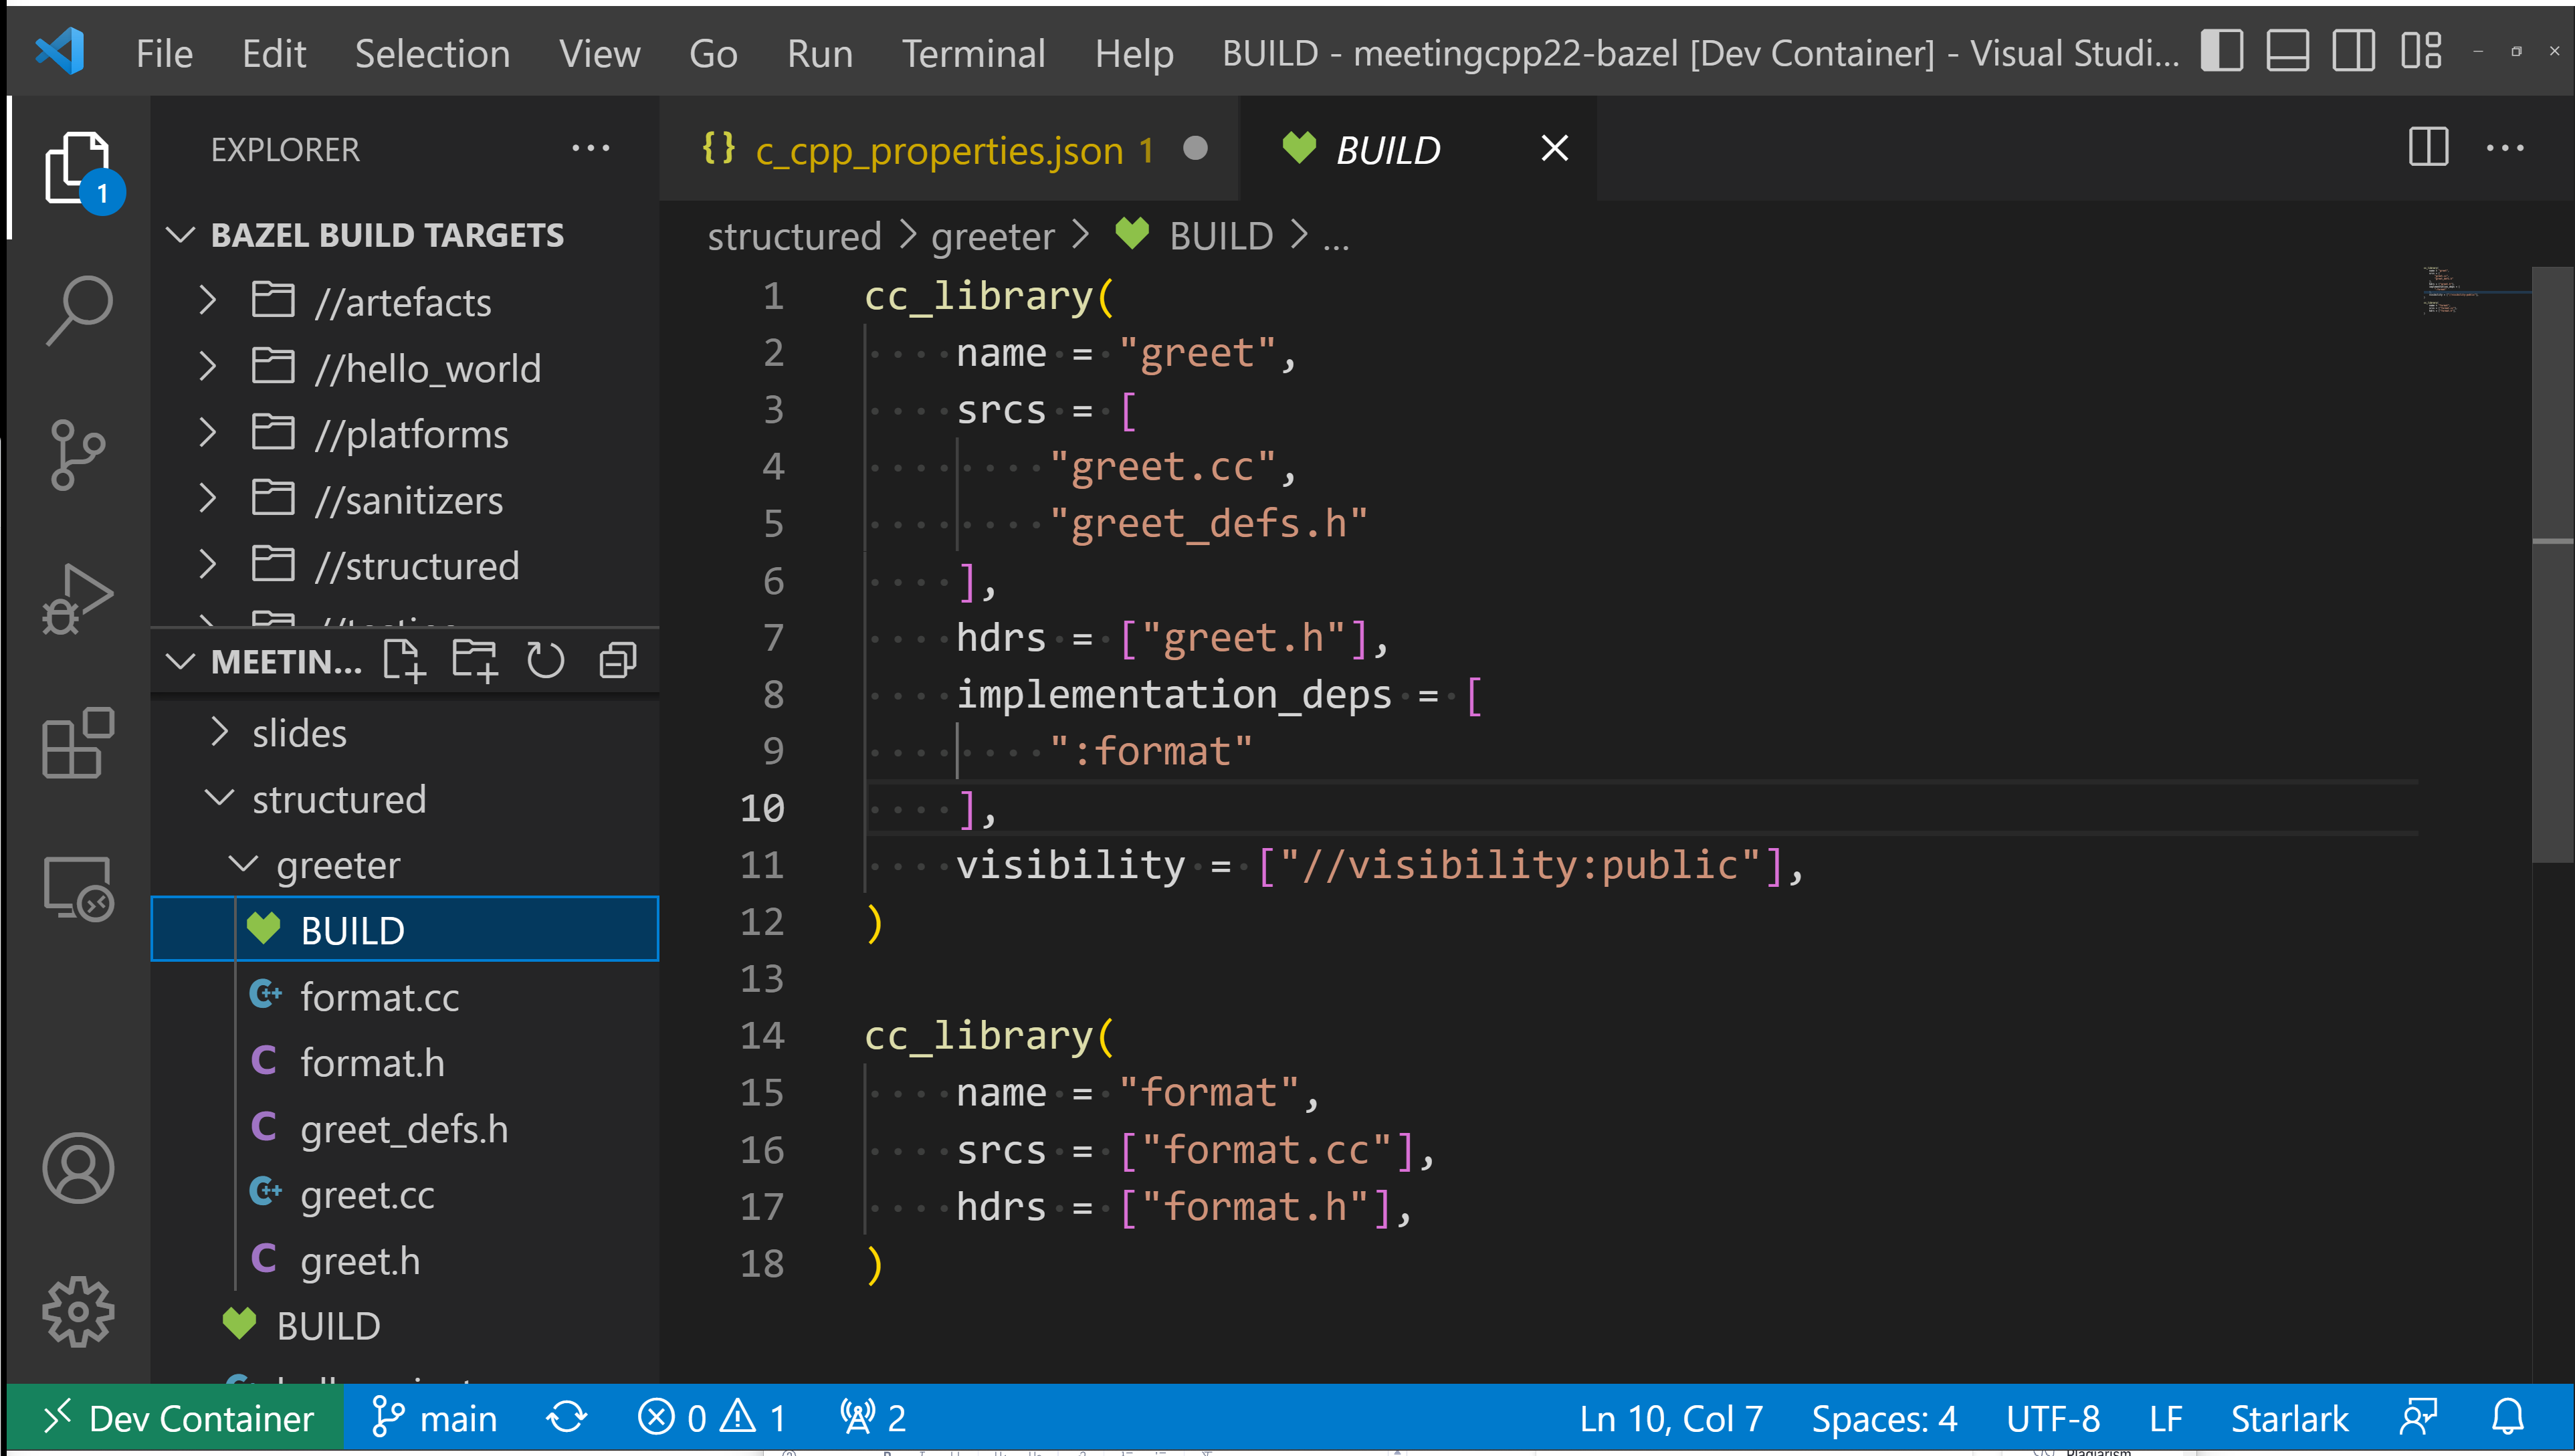
\includegraphics[width=\paperwidth]{slides/static_demos/01_03_greeter_BUILD.png}}
\begin{frame}[plain]
\end{frame}
}

{
\usebackgroundtemplate{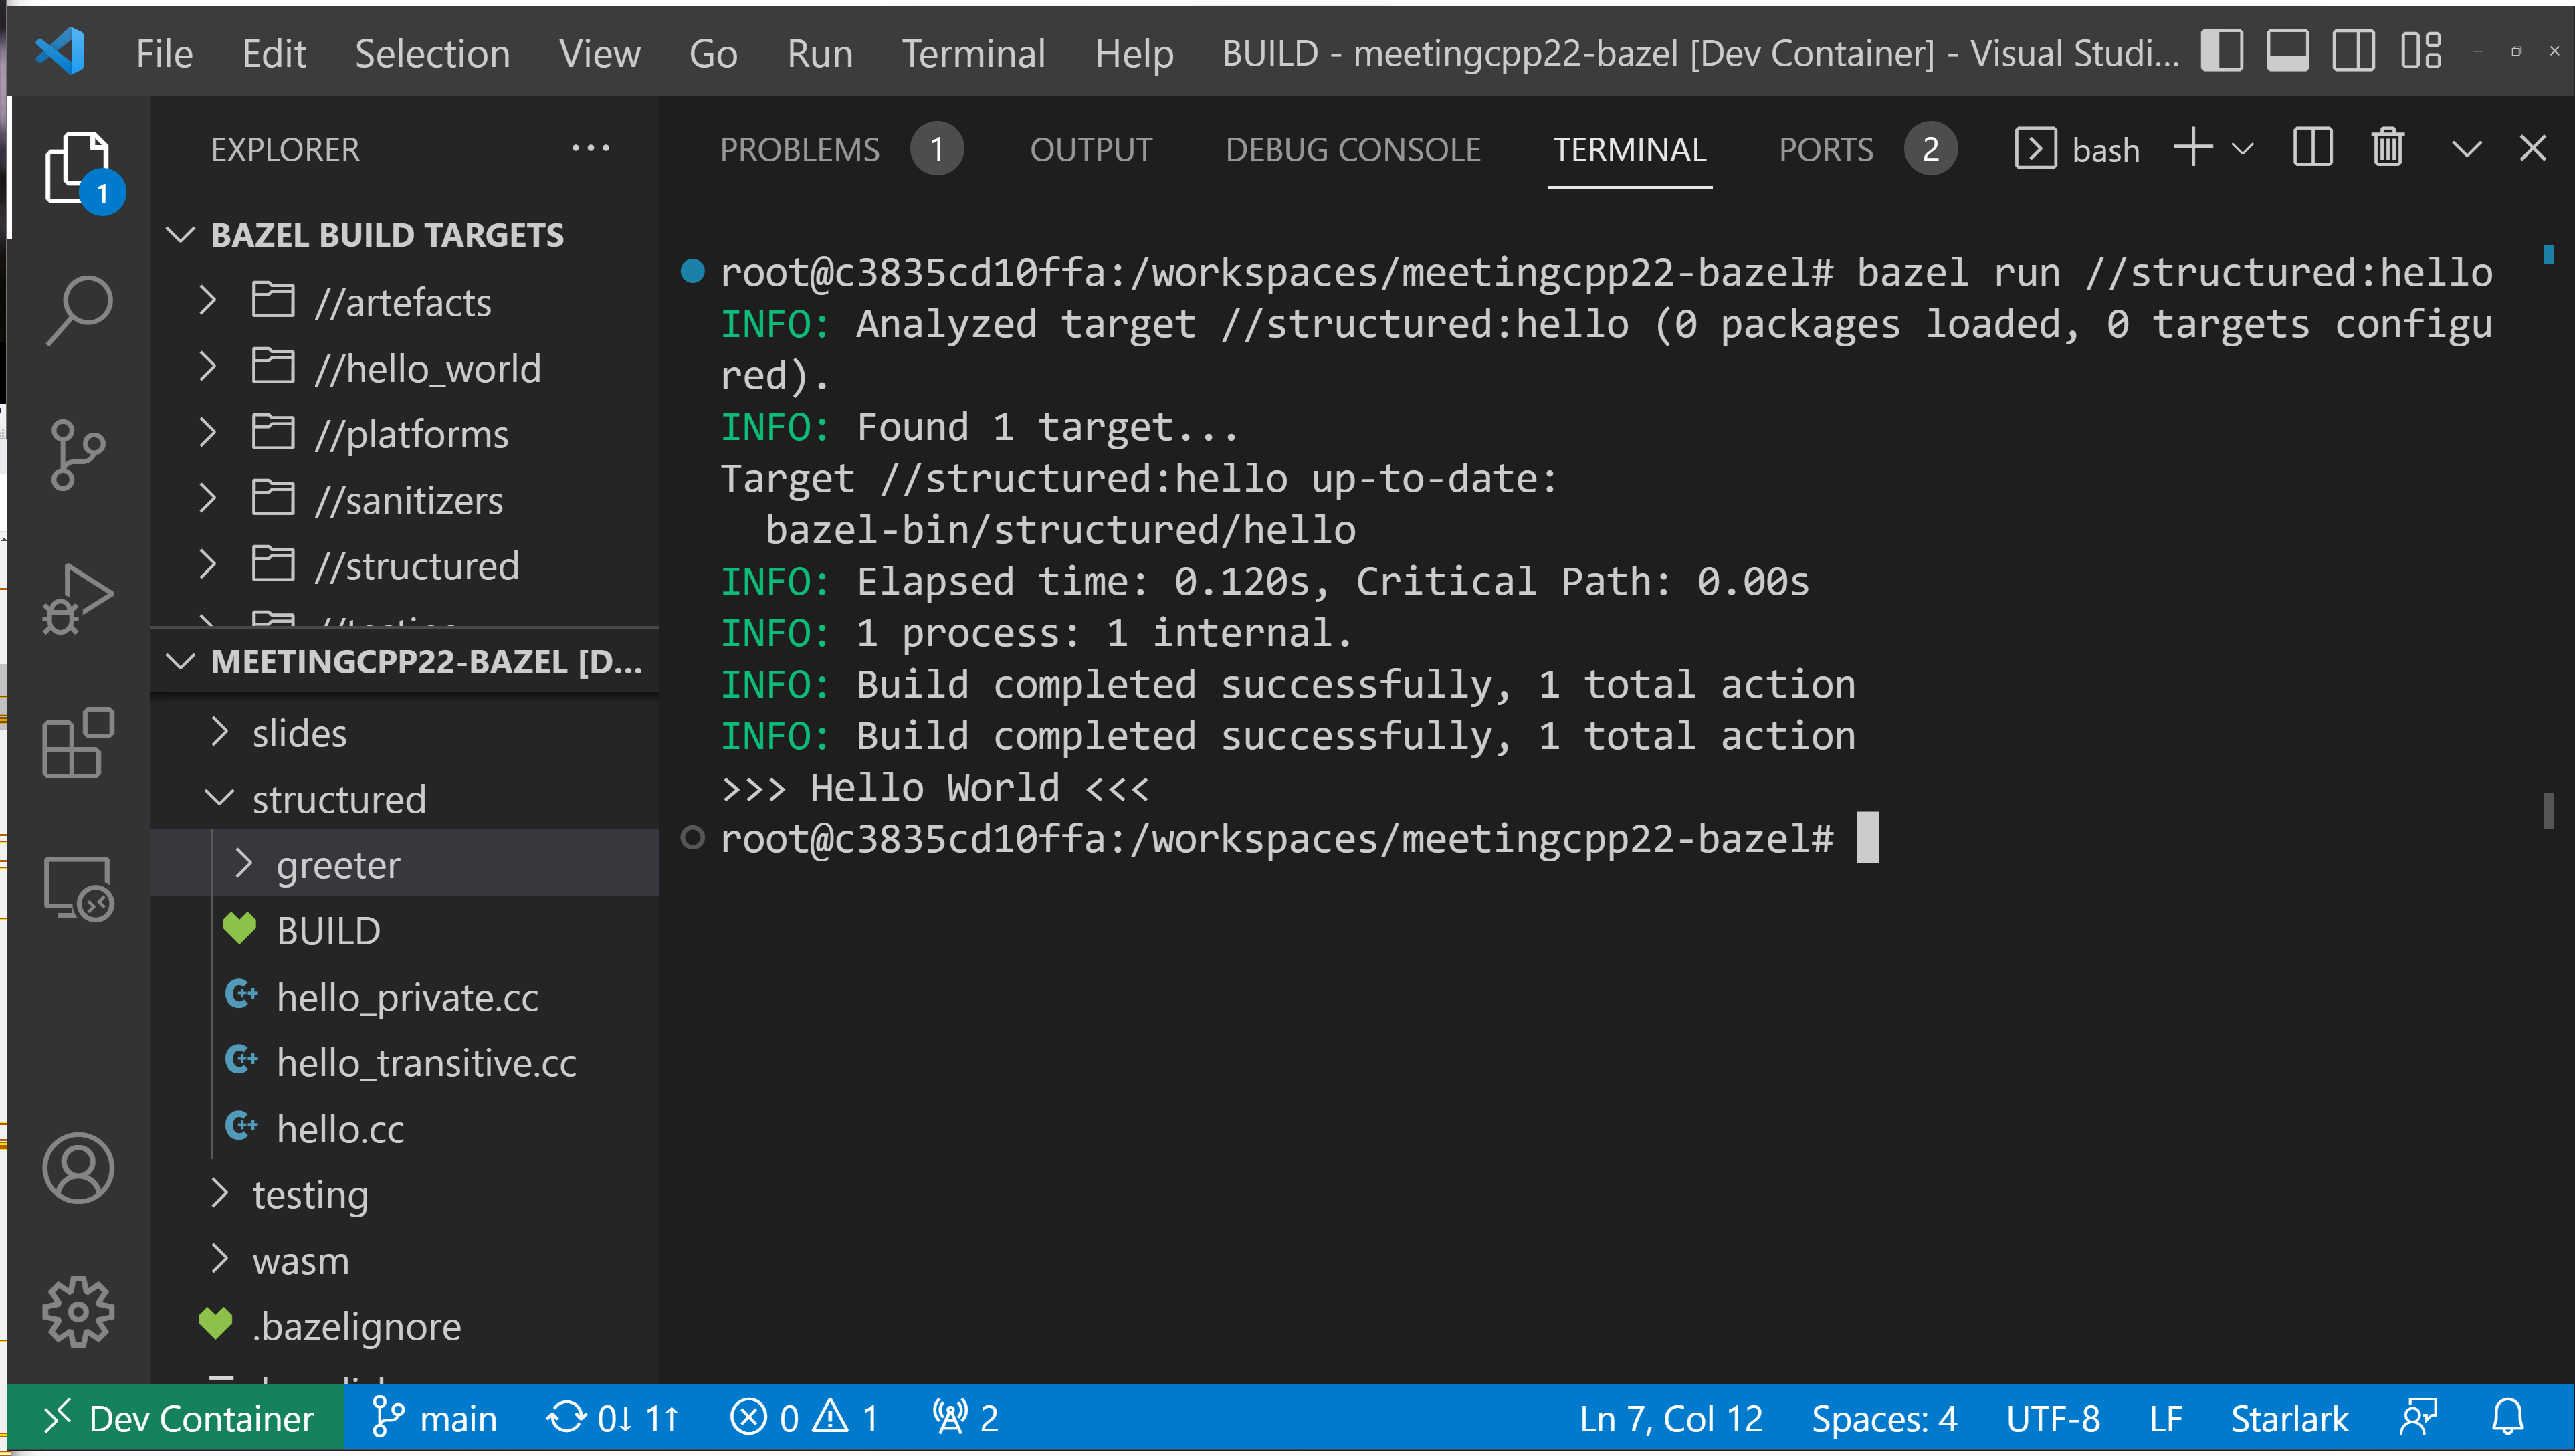
\includegraphics[width=\paperwidth]{slides/static_demos/01_04_run.png}}
\begin{frame}[plain]
\end{frame}
}

{
\usebackgroundtemplate{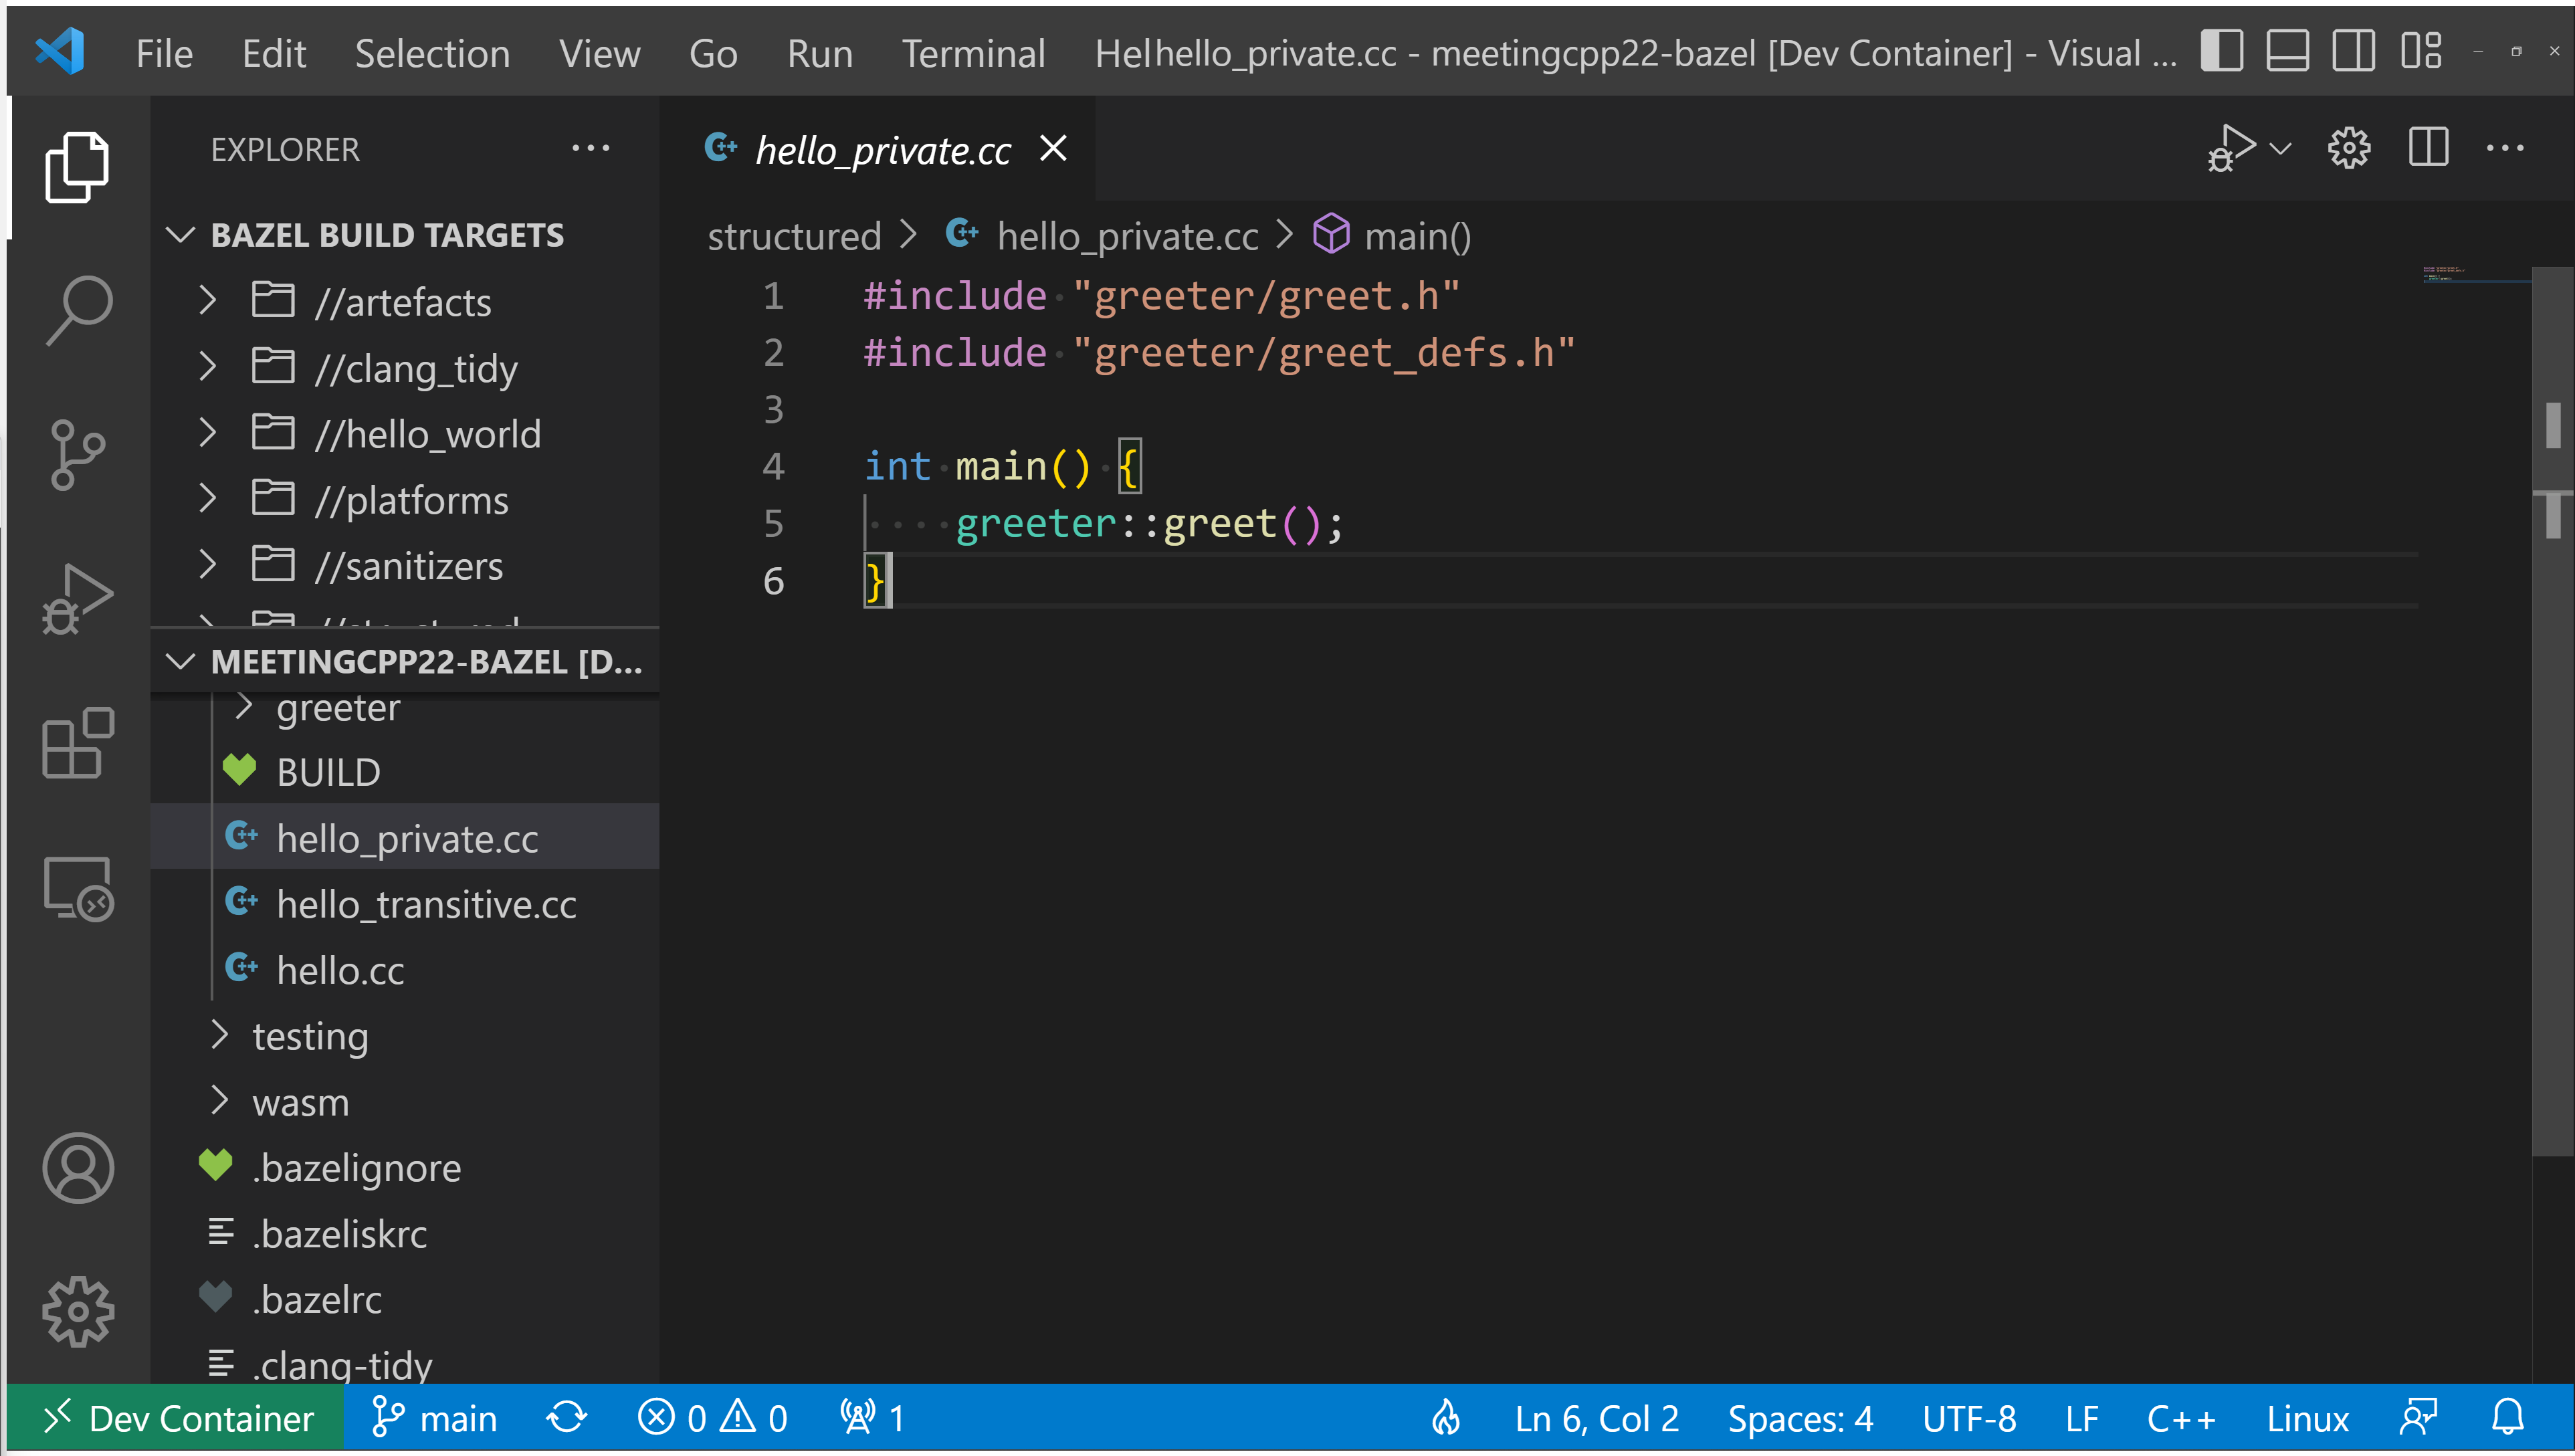
\includegraphics[width=\paperwidth]{slides/static_demos/01_05_private.png}}
\begin{frame}[plain]
\end{frame}
}

{
\usebackgroundtemplate{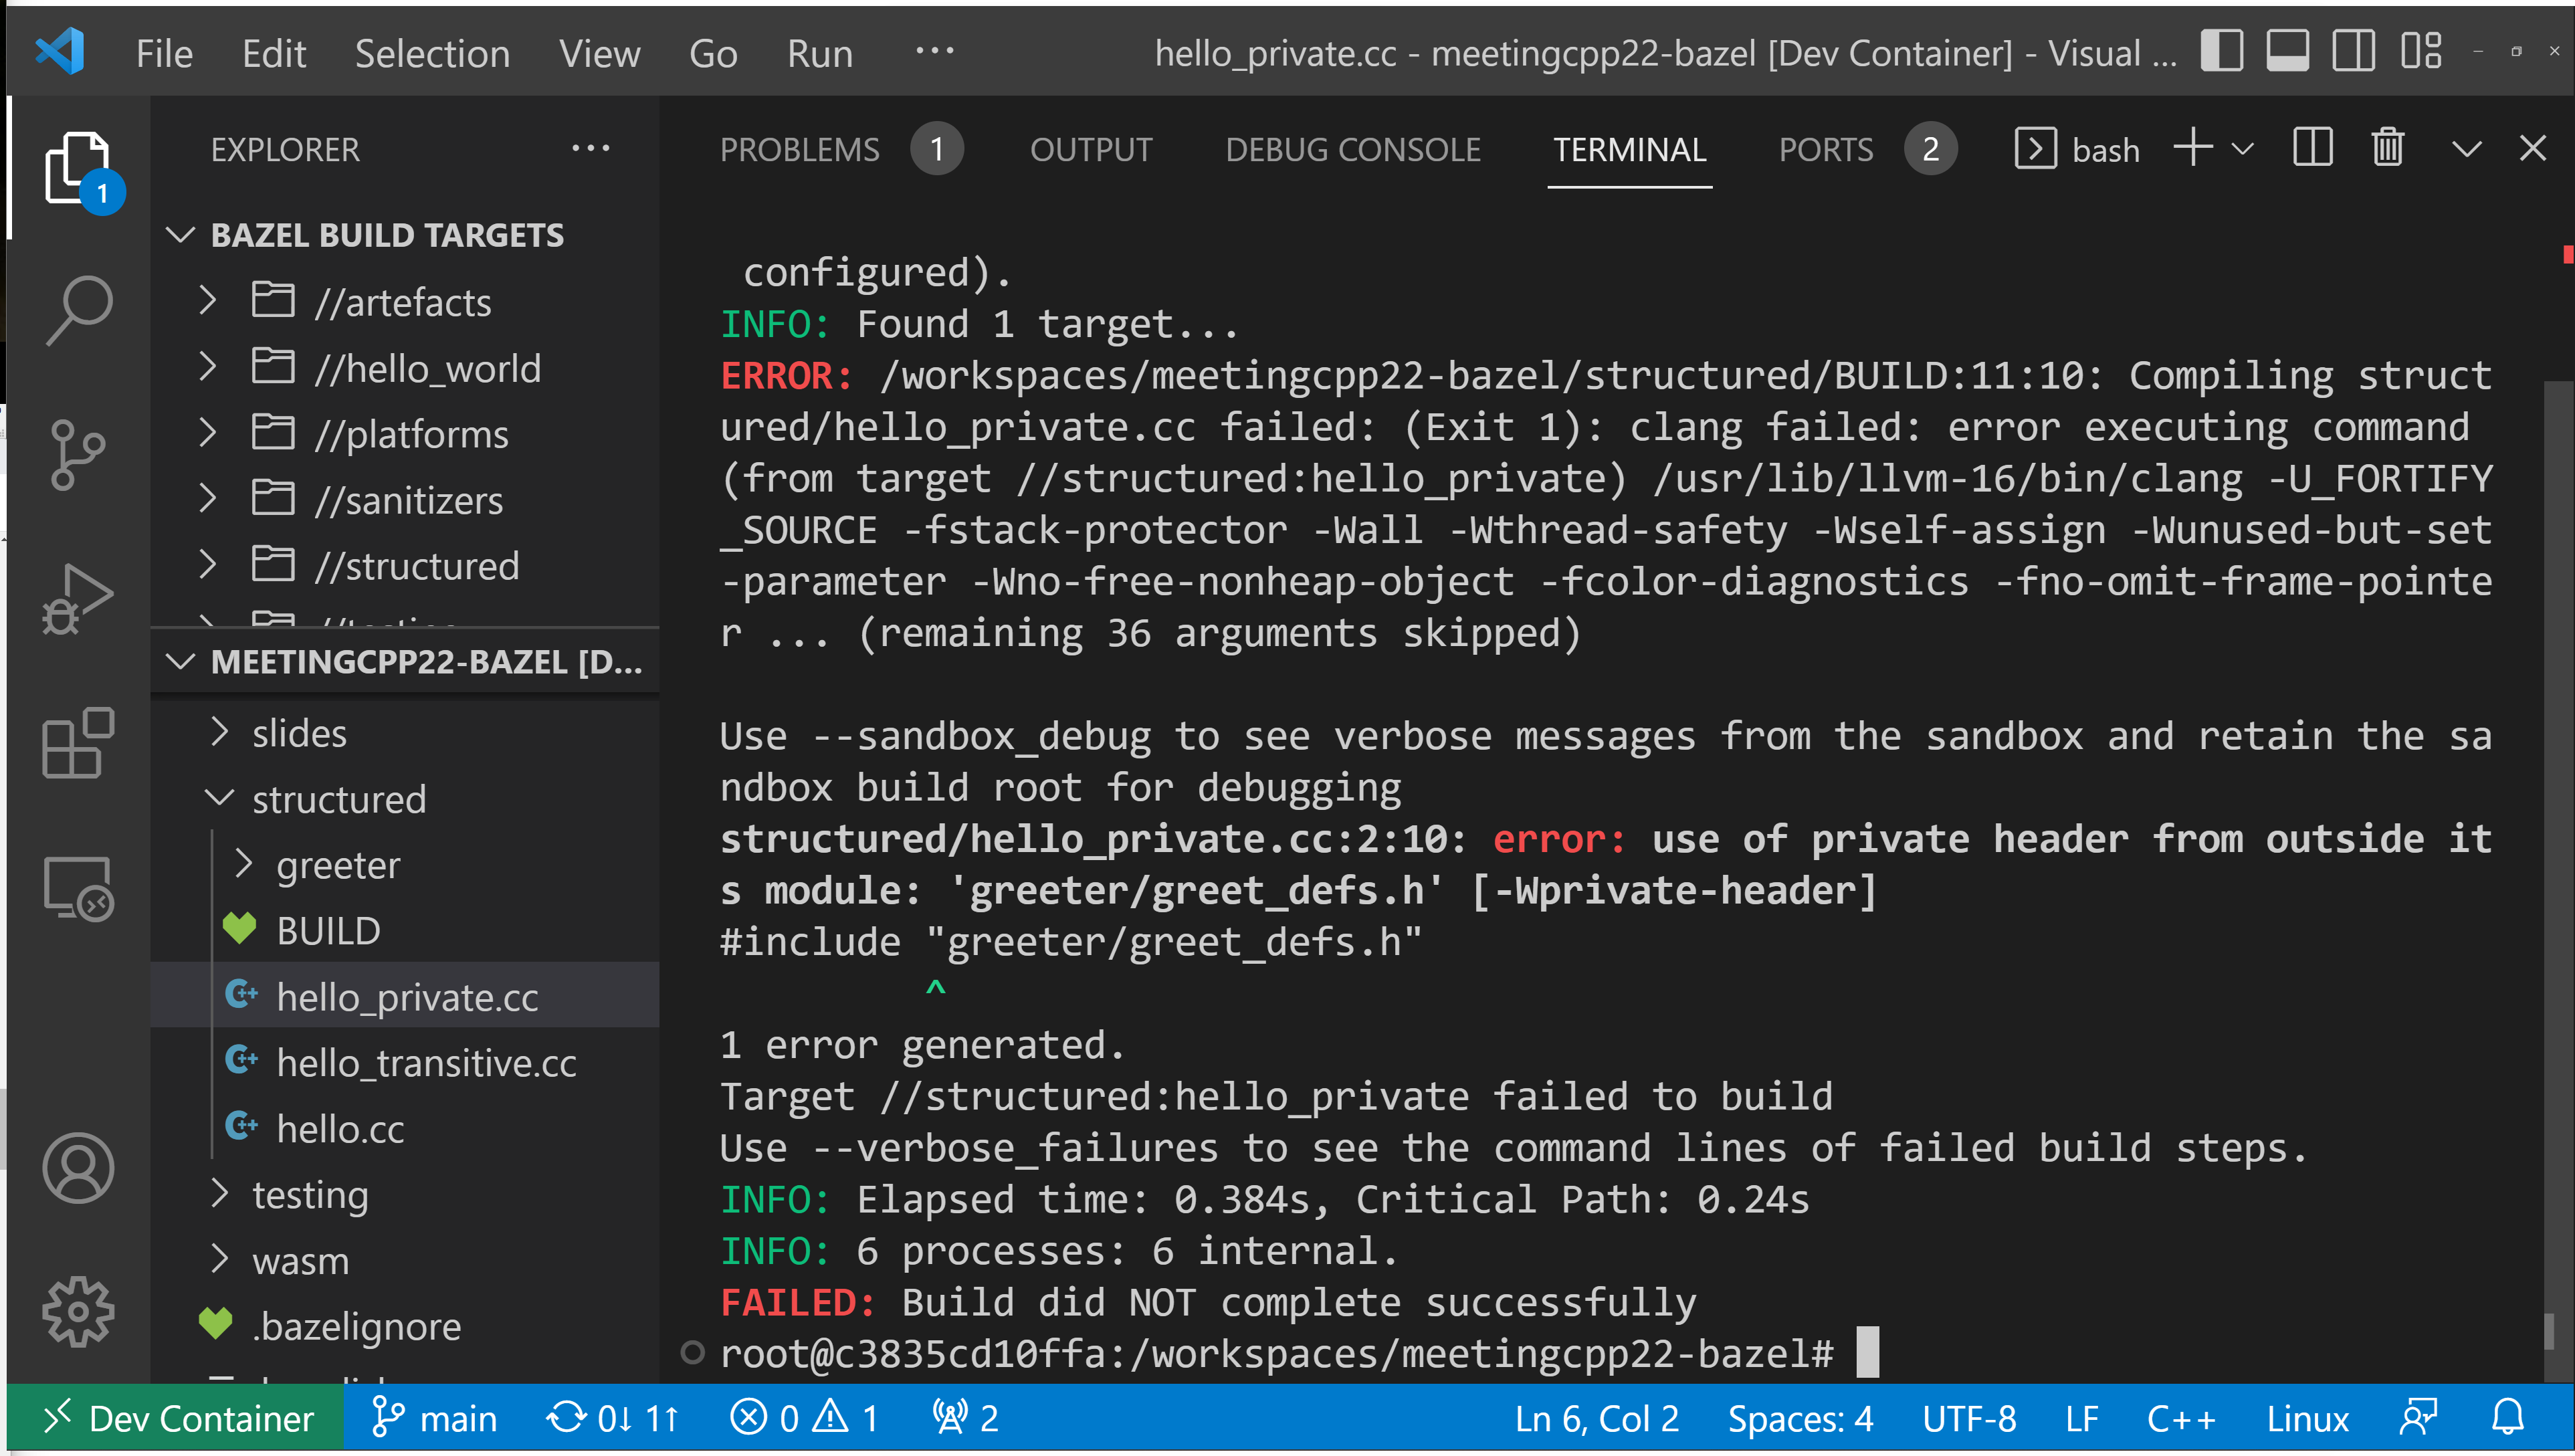
\includegraphics[width=\paperwidth]{slides/static_demos/01_06_private_build.png}}
\begin{frame}[plain]
\end{frame}
}

{
\usebackgroundtemplate{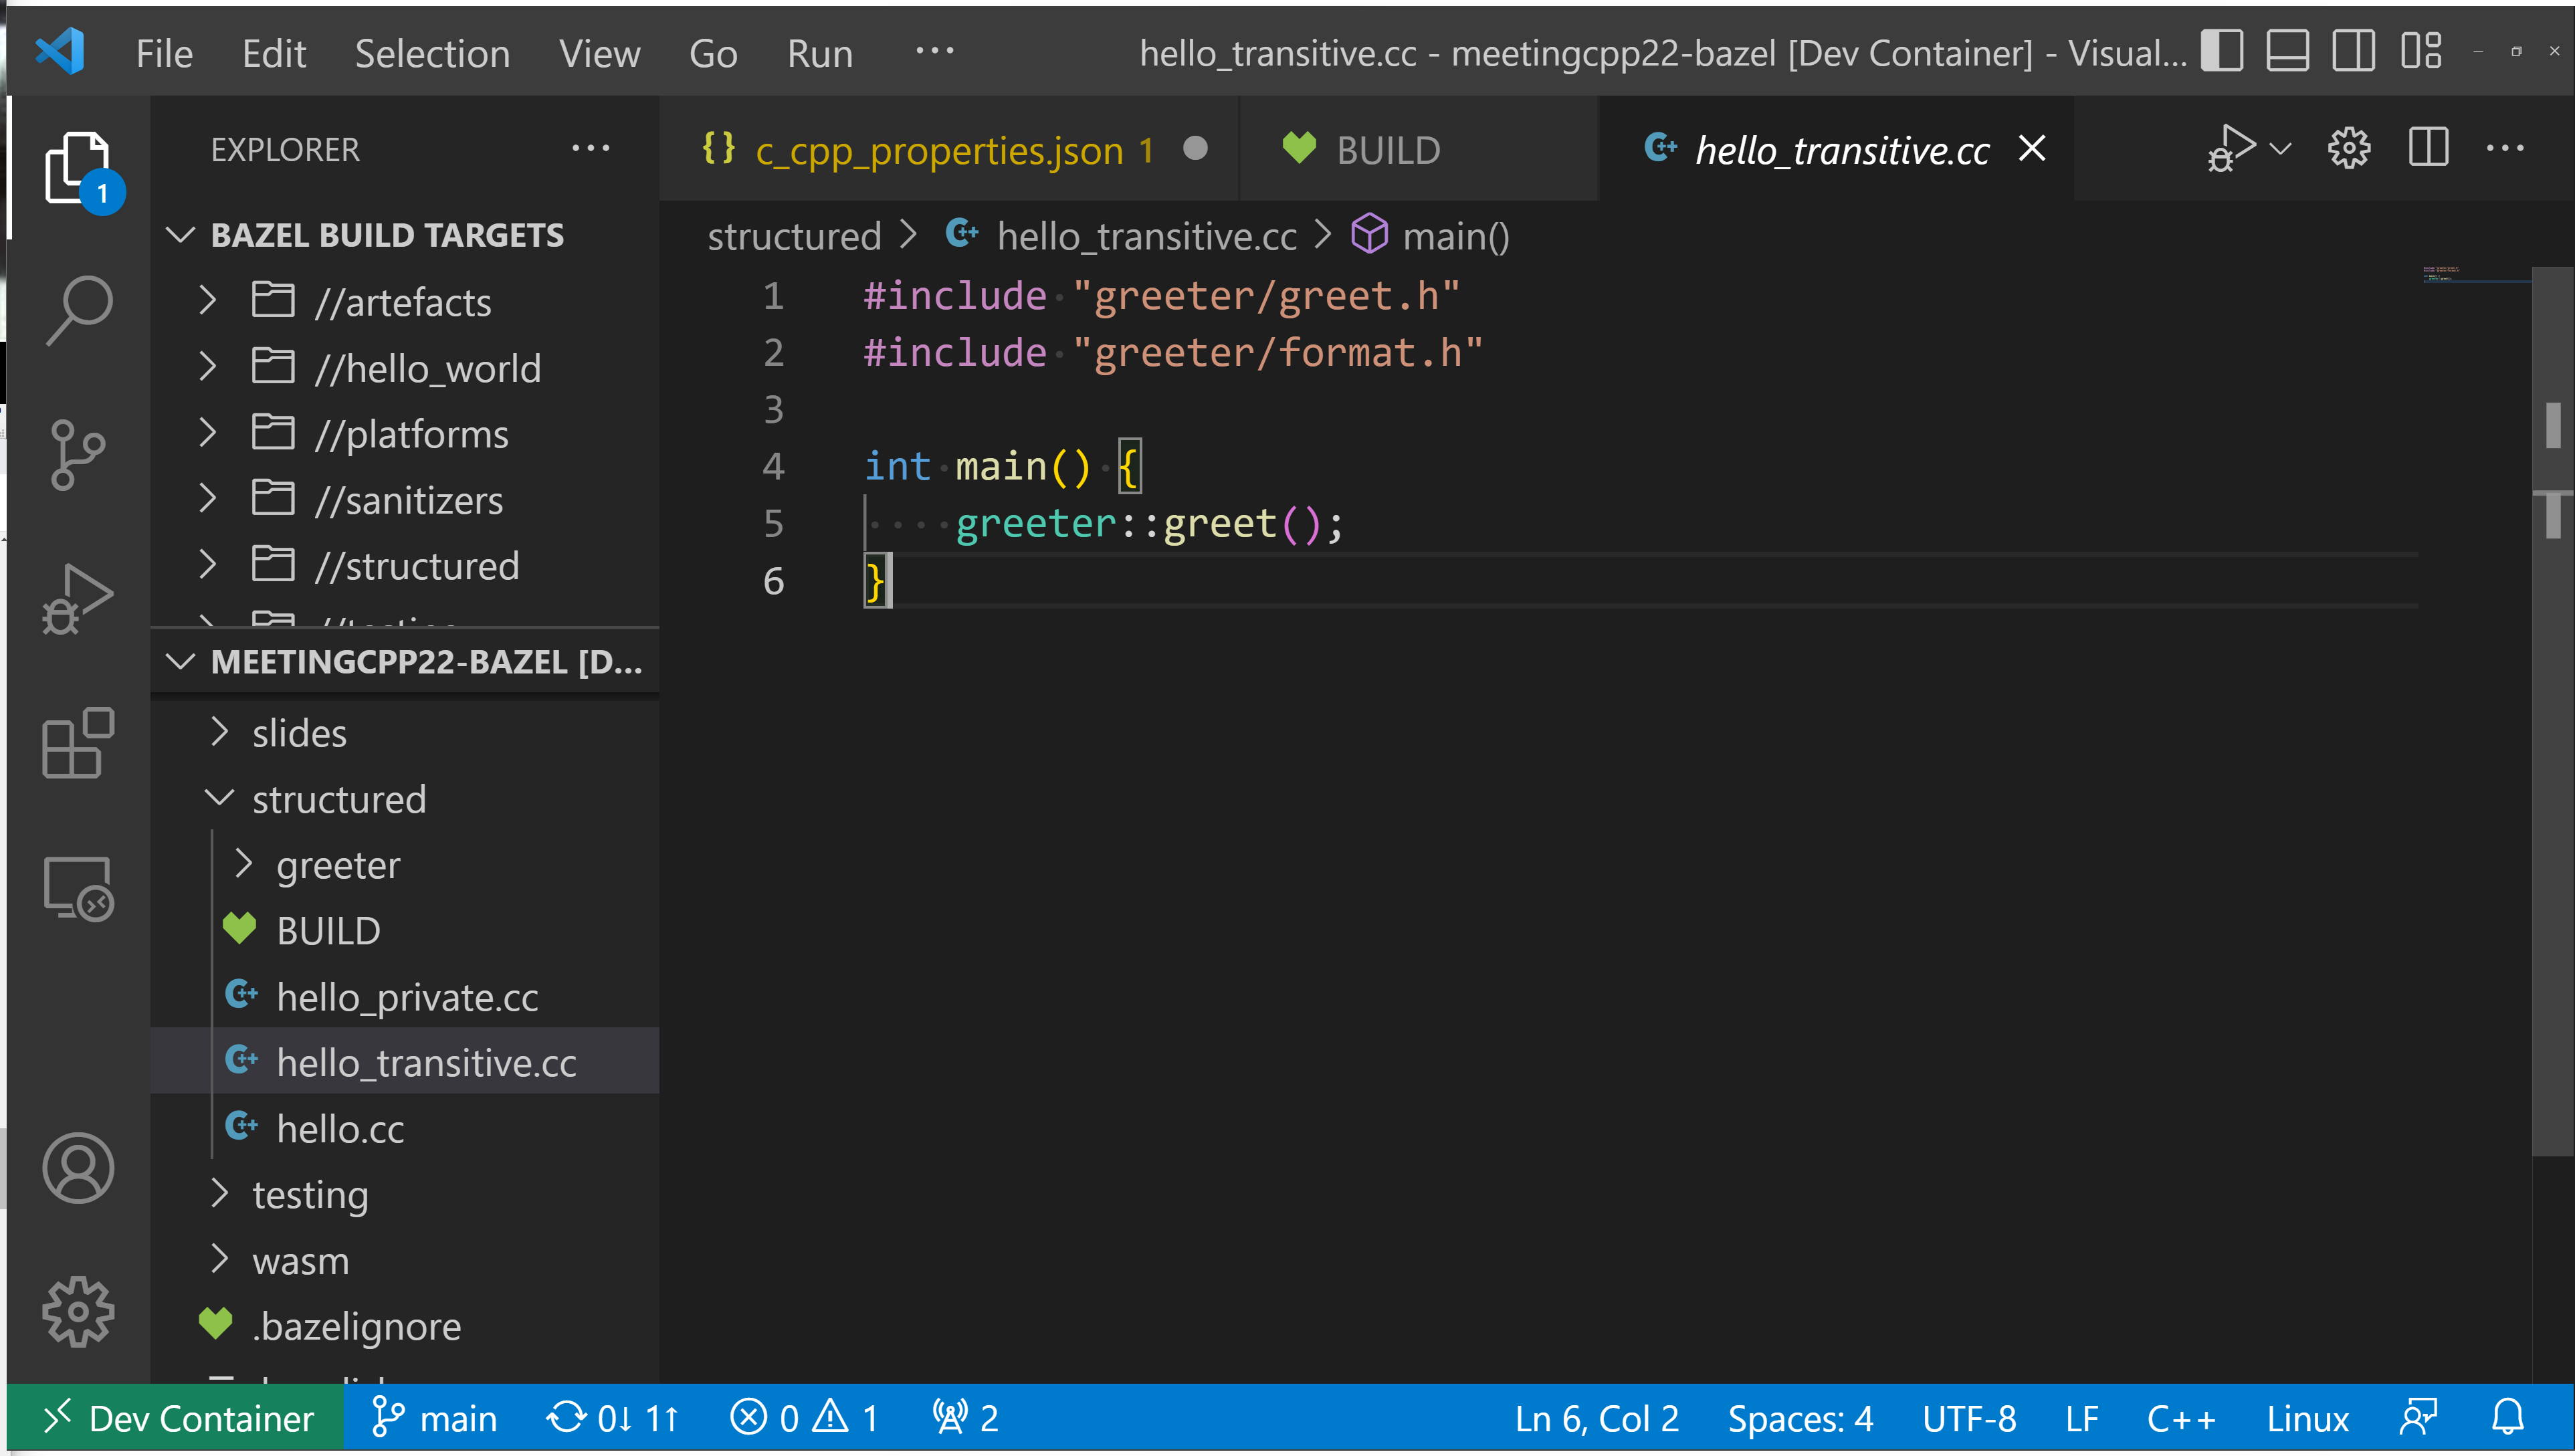
\includegraphics[width=\paperwidth]{slides/static_demos/01_07_transitive.png}}
\begin{frame}[plain]
\end{frame}
}

{
\usebackgroundtemplate{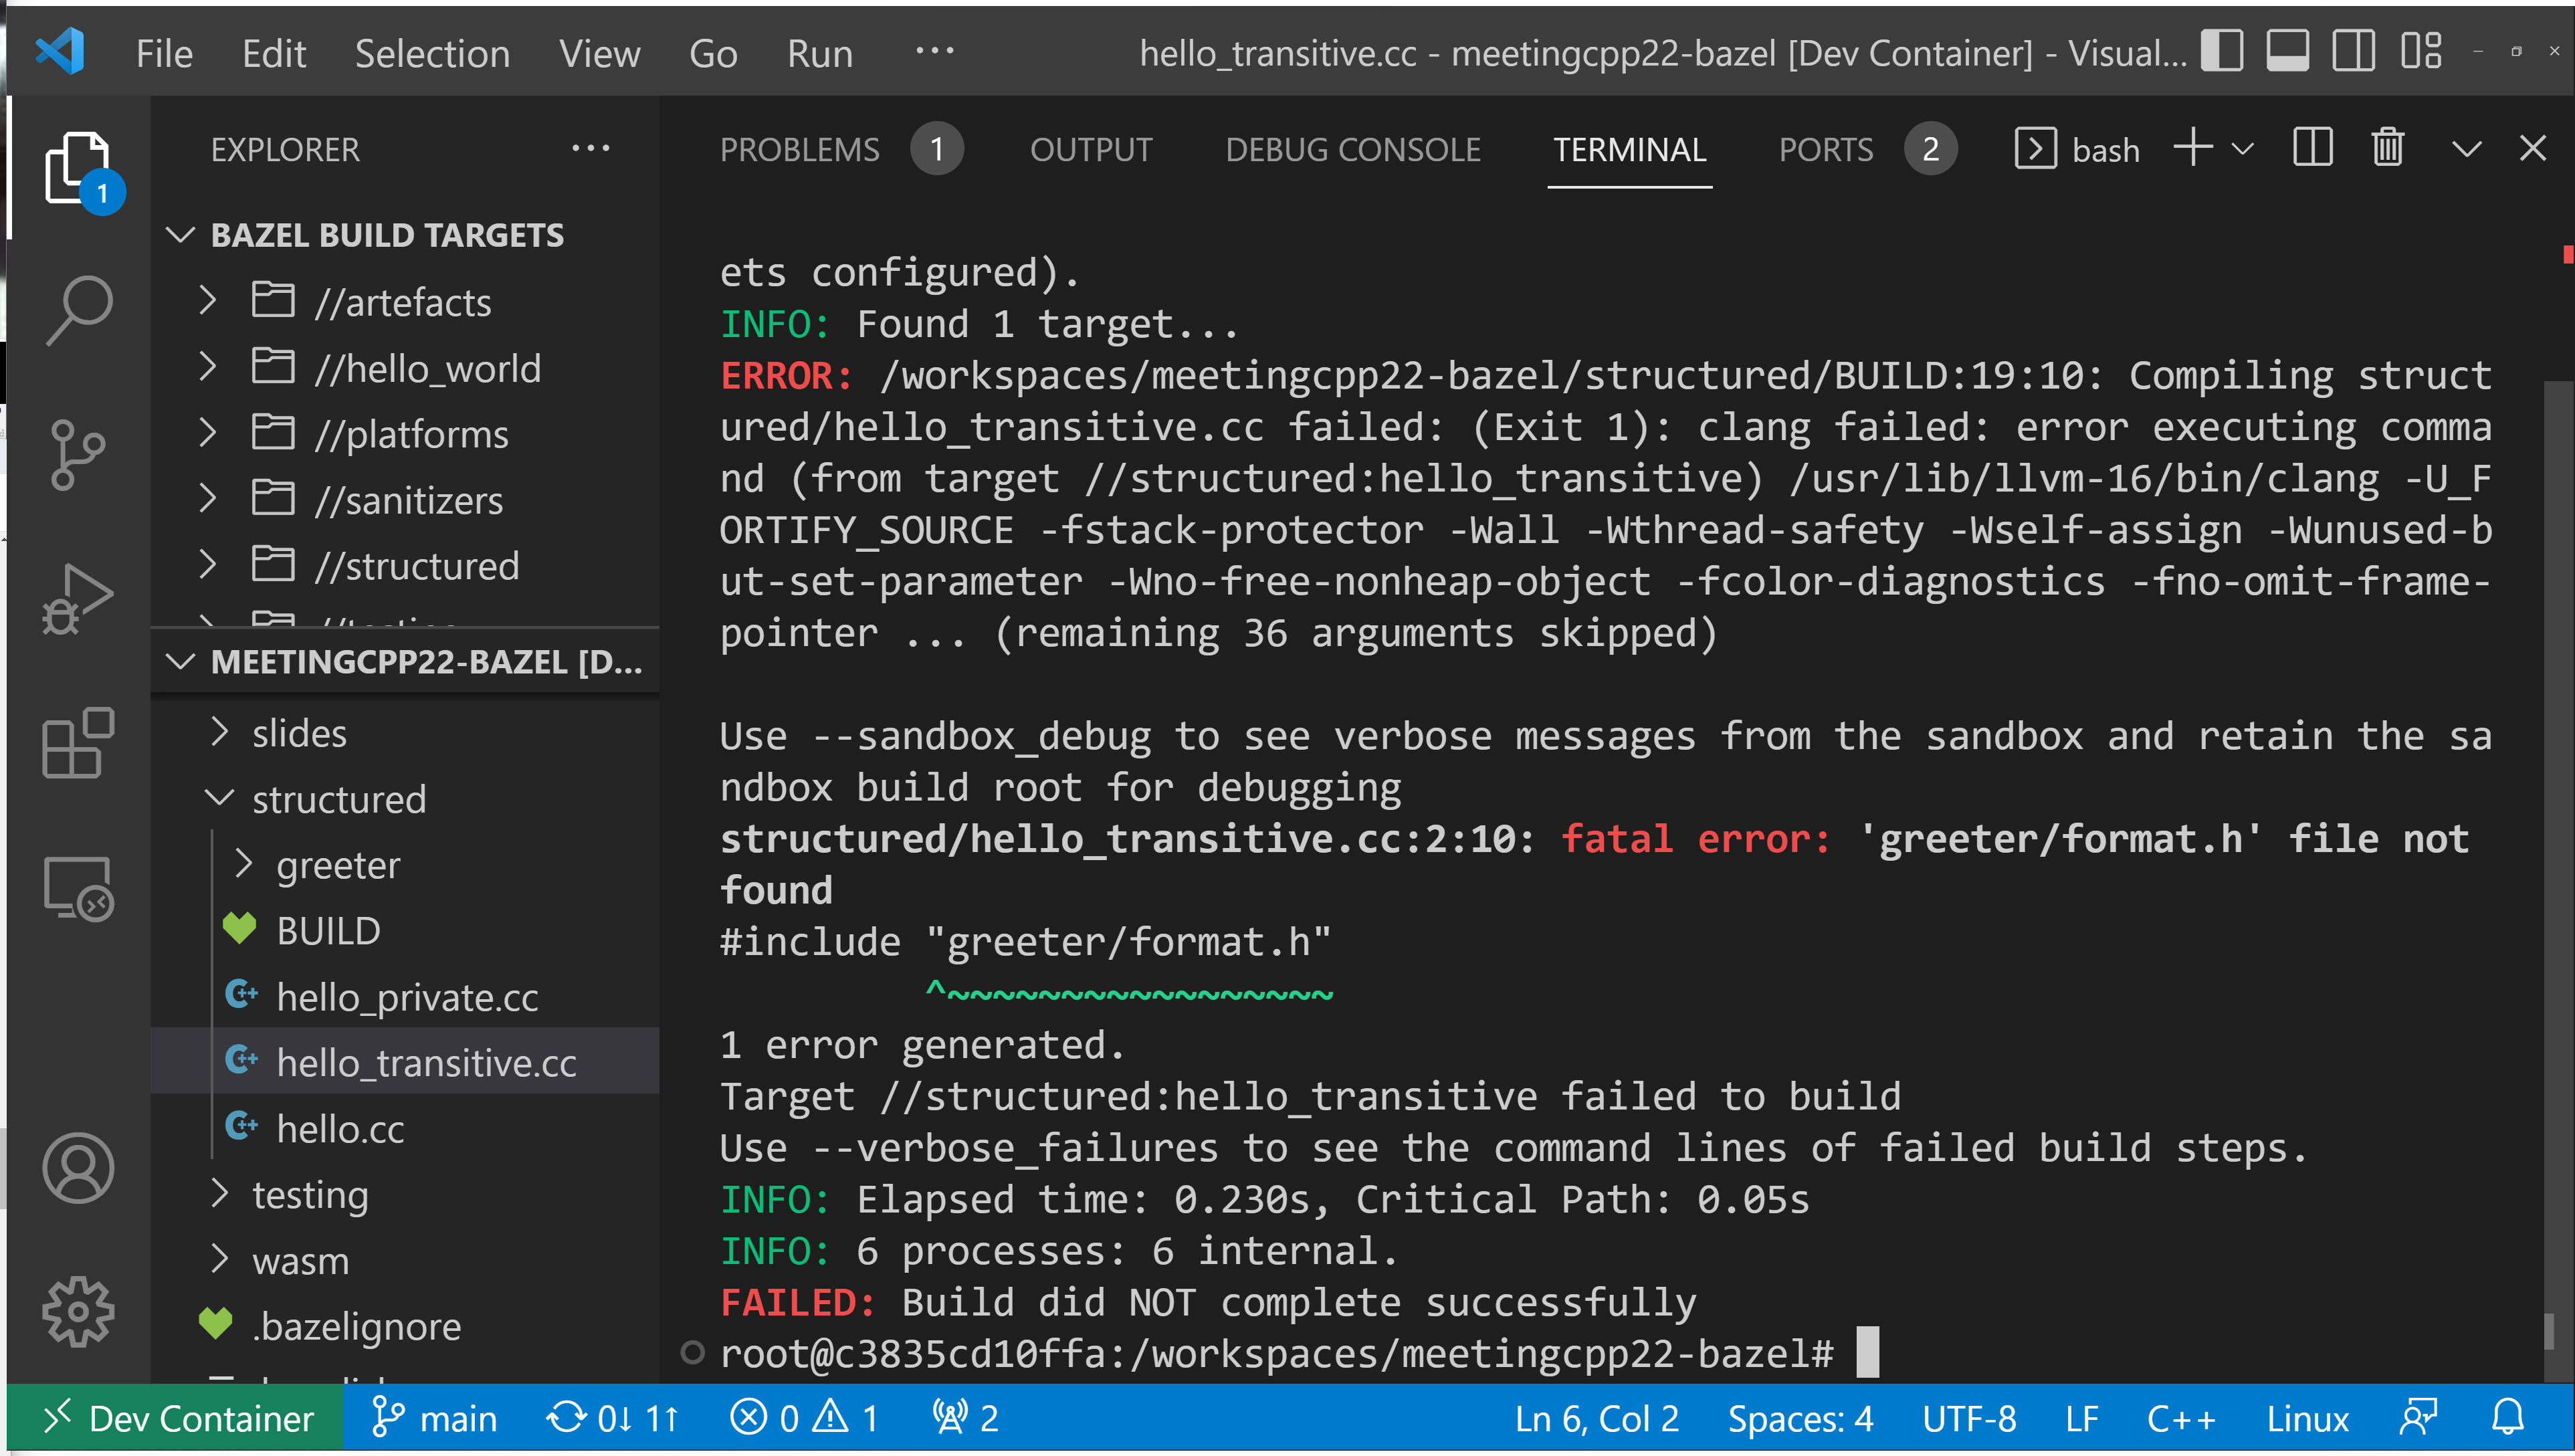
\includegraphics[width=\paperwidth]{slides/static_demos/01_08_transitive_build.png}}
\begin{frame}[plain]
\end{frame}
}

{
\usebackgroundtemplate{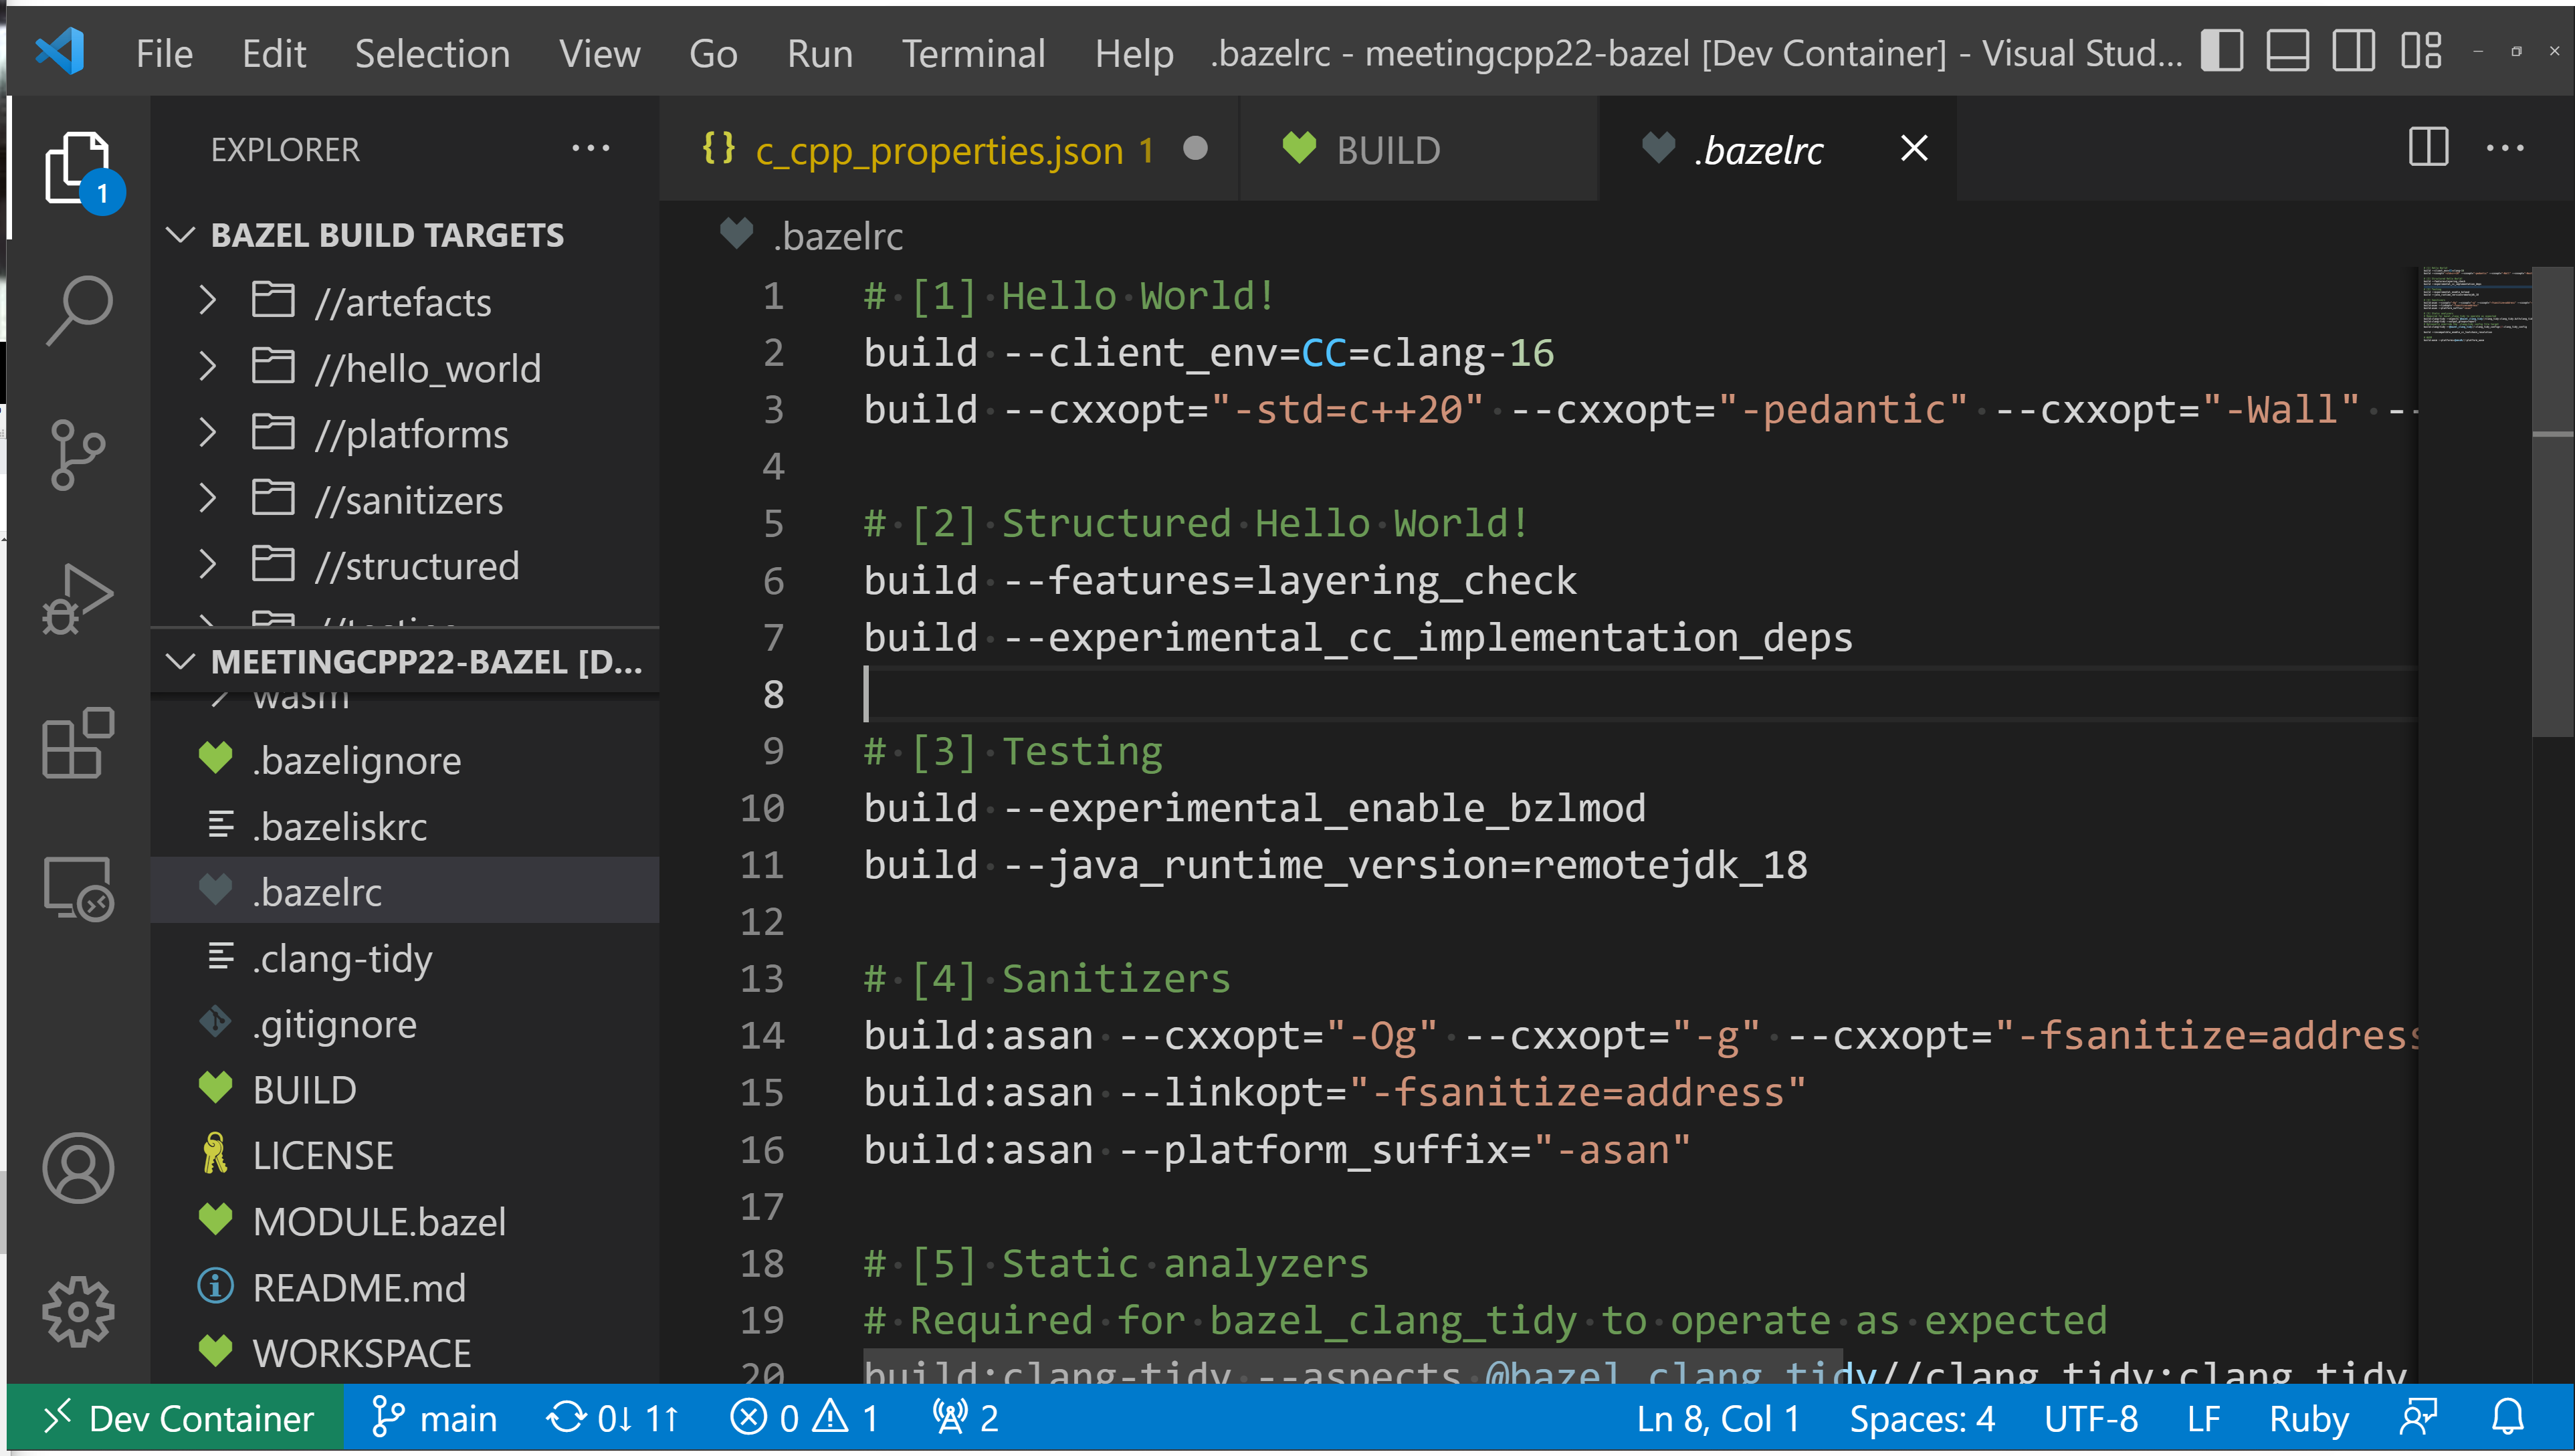
\includegraphics[width=\paperwidth]{slides/static_demos/01_09_bazelrc.png}}
\begin{frame}[plain]
\end{frame}
}

\begin{frame}{}
    \begin{center}
        \begin{Huge}Testing\end{Huge}
    \end{center}
\end{frame}

{
\usebackgroundtemplate{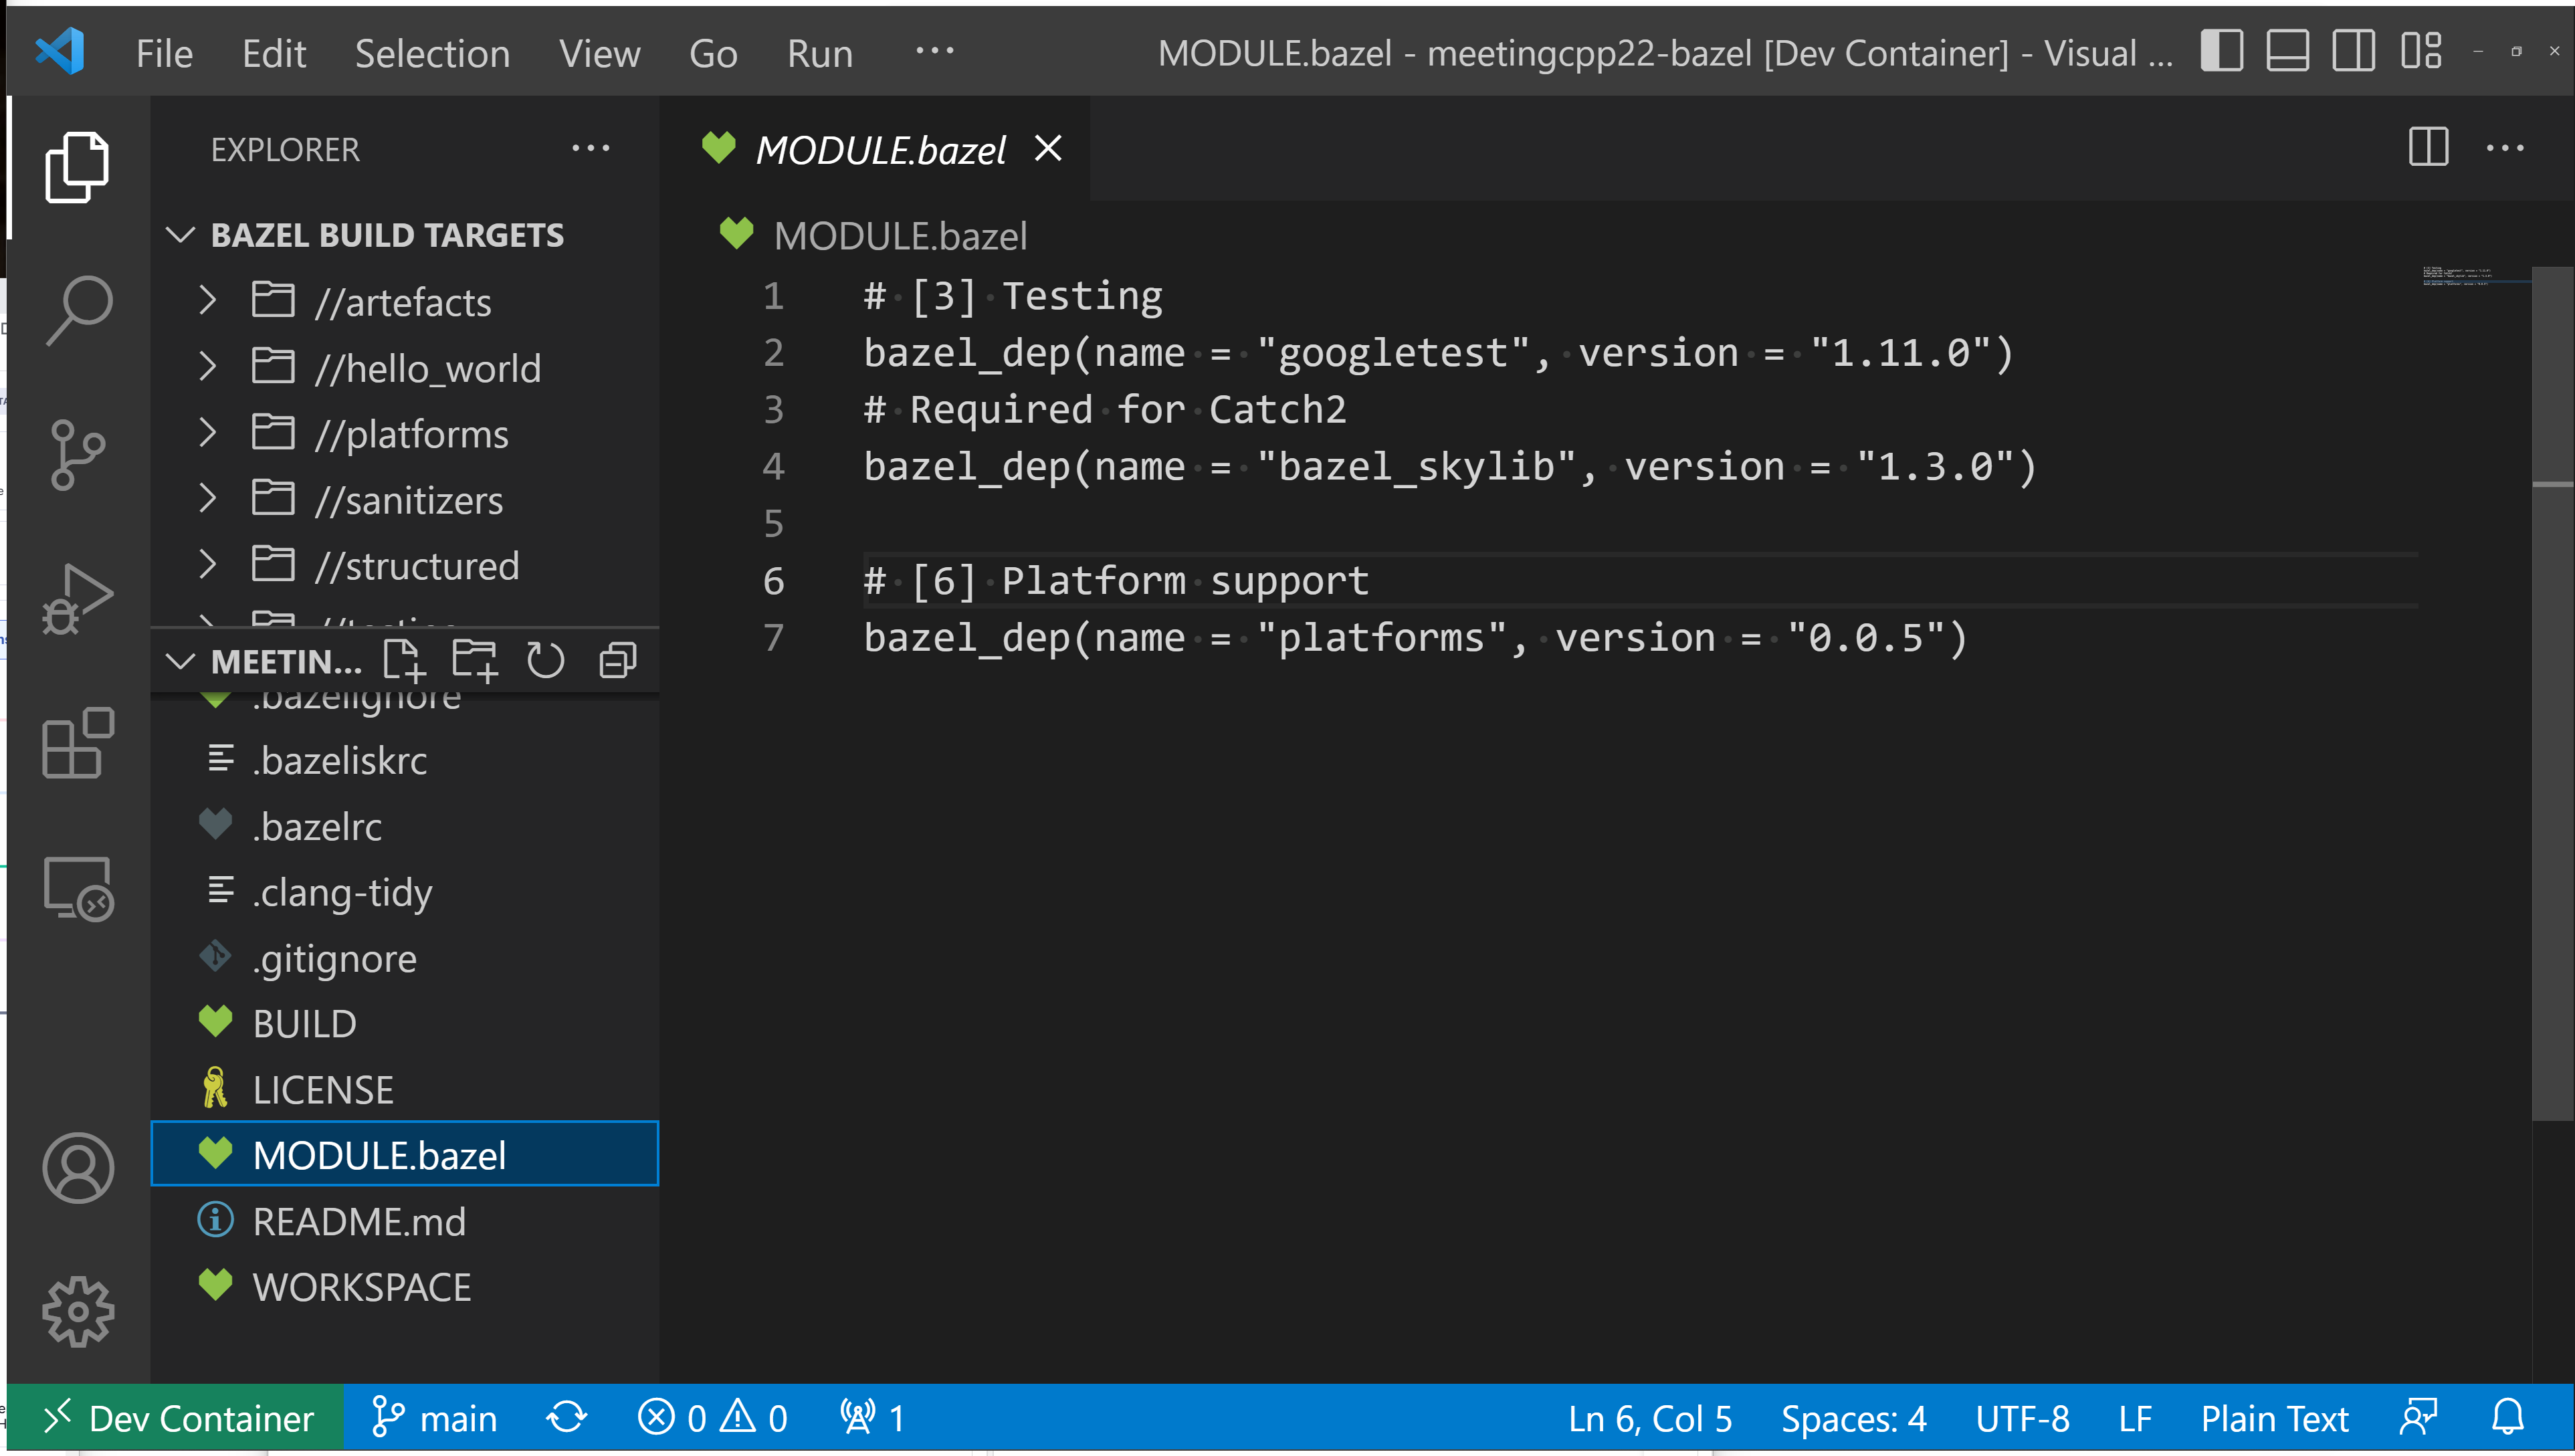
\includegraphics[width=\paperwidth]{slides/static_demos/02_01_modules.png}}
\begin{frame}[plain]
\end{frame}
}

{
\usebackgroundtemplate{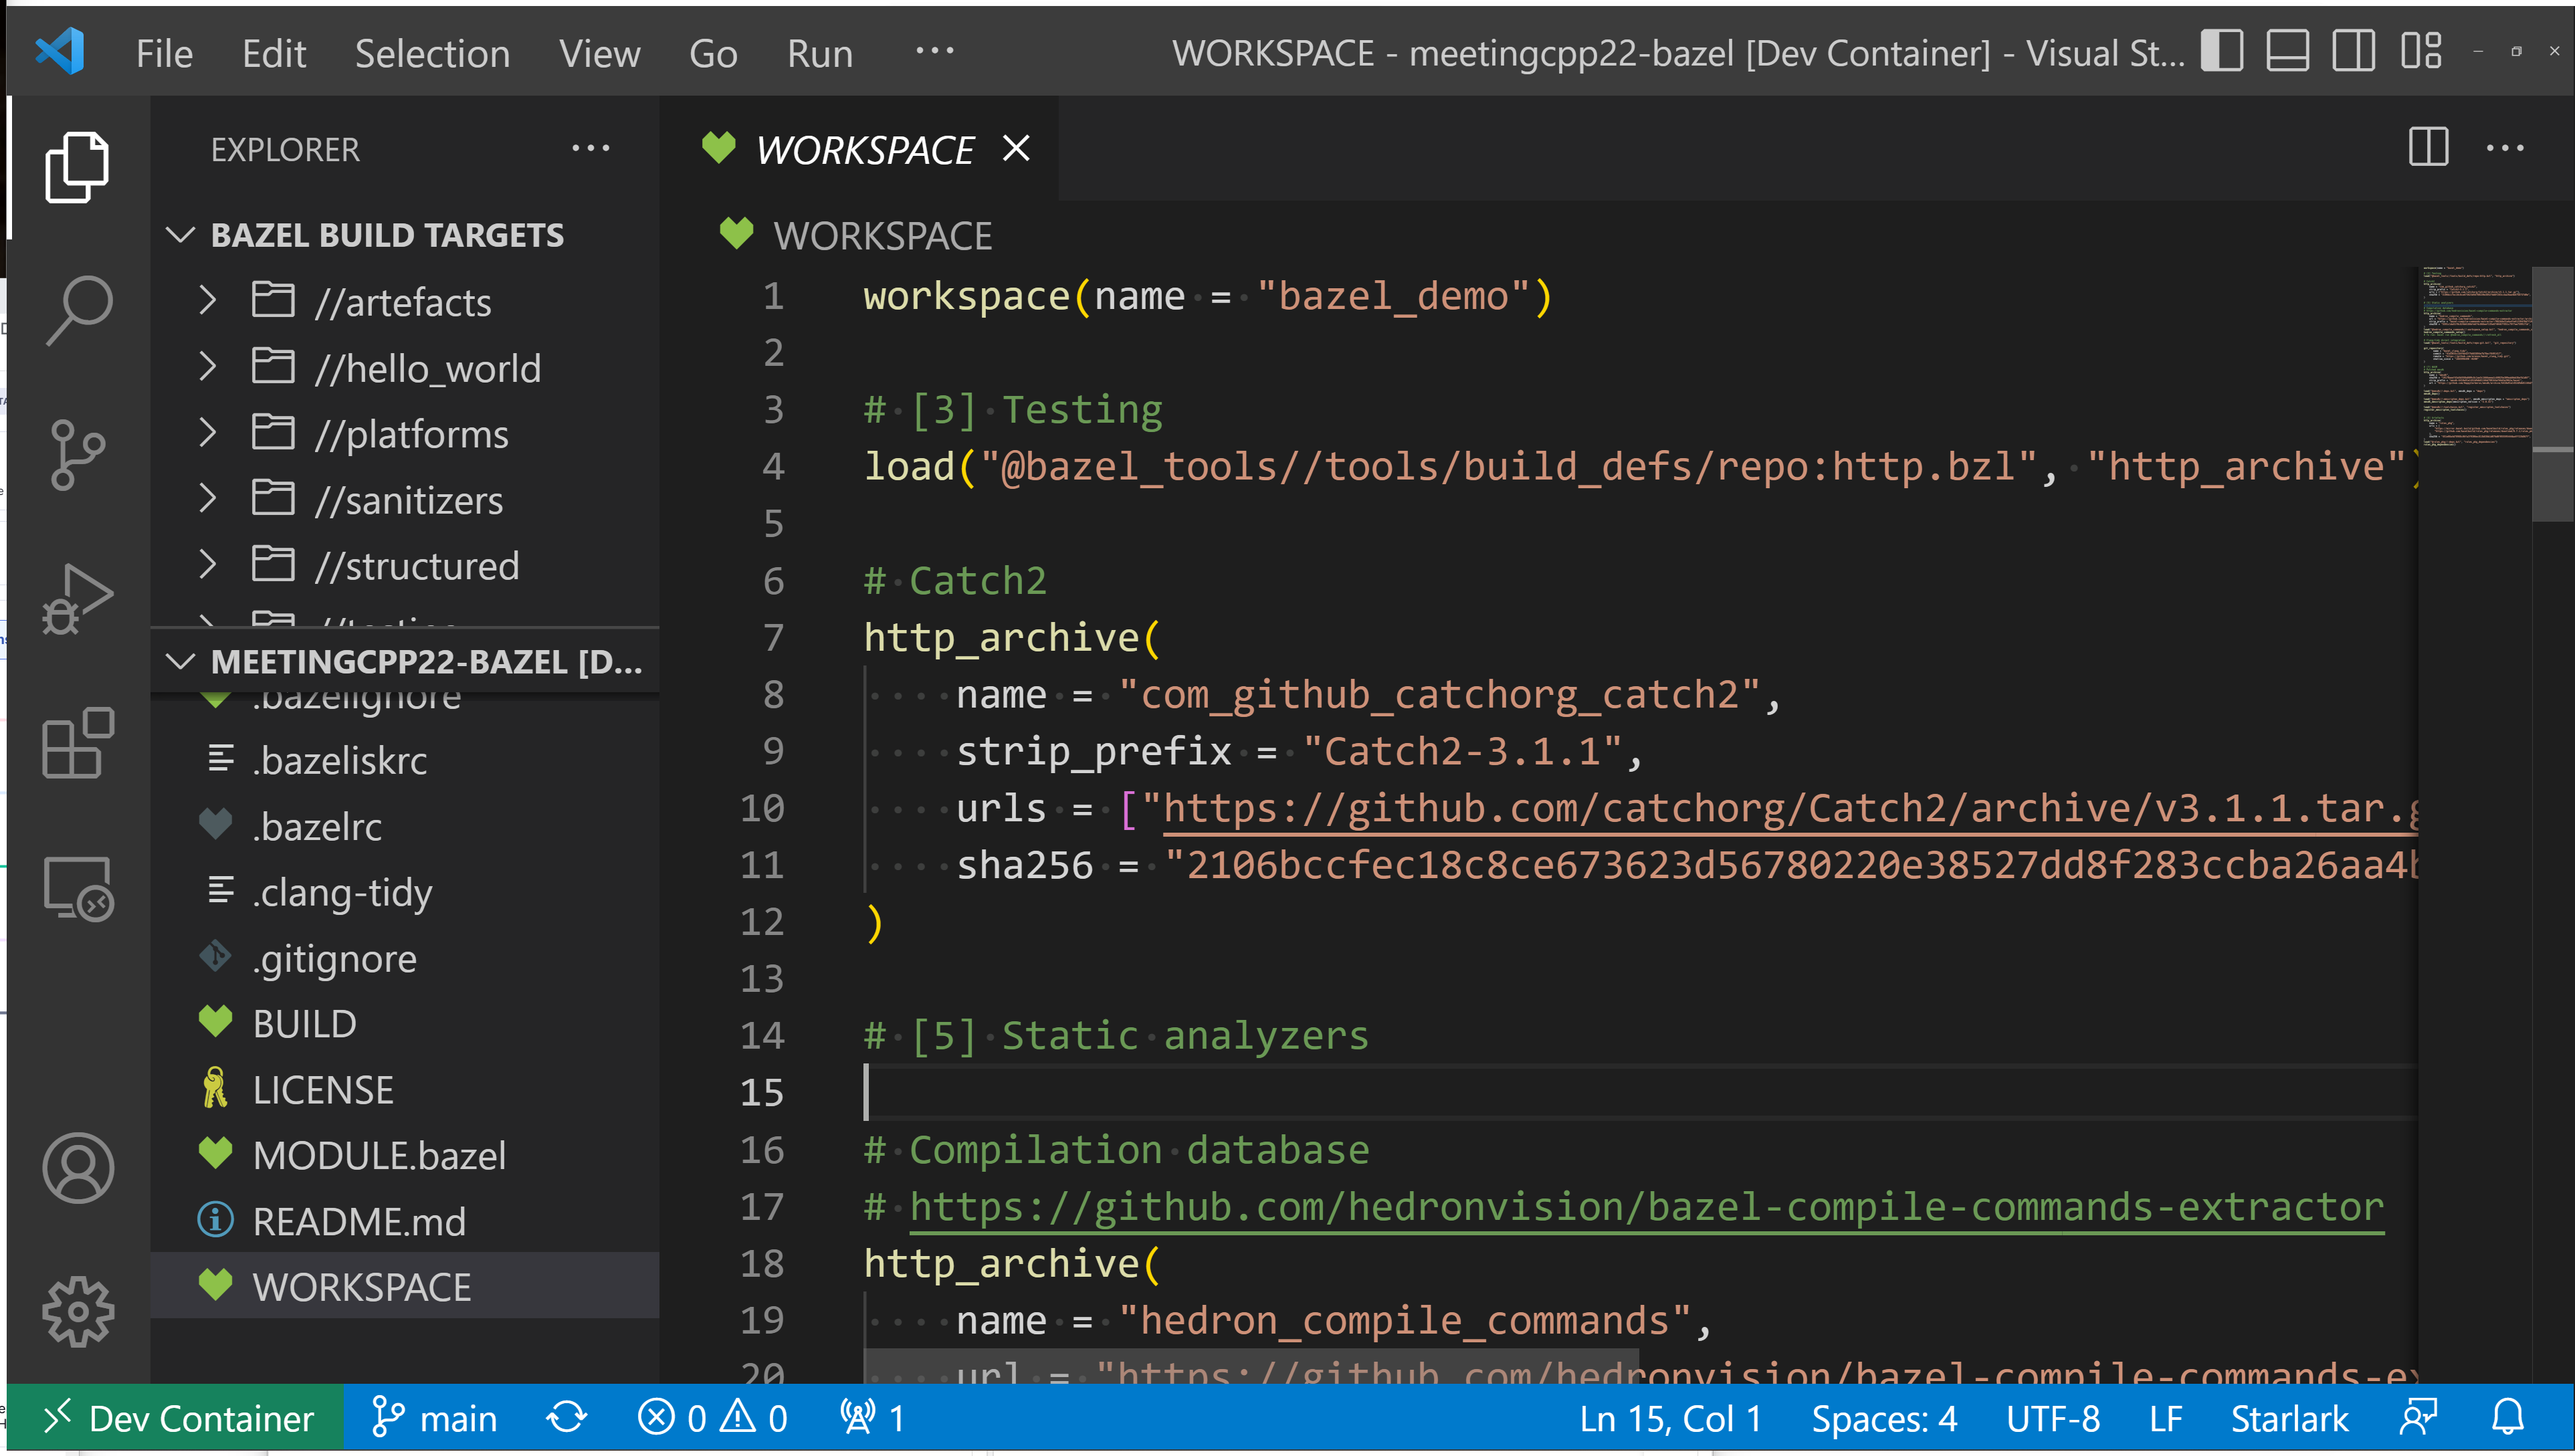
\includegraphics[width=\paperwidth]{slides/static_demos/02_02_manual_dep.png}}
\begin{frame}[plain]
\end{frame}
}

{
\usebackgroundtemplate{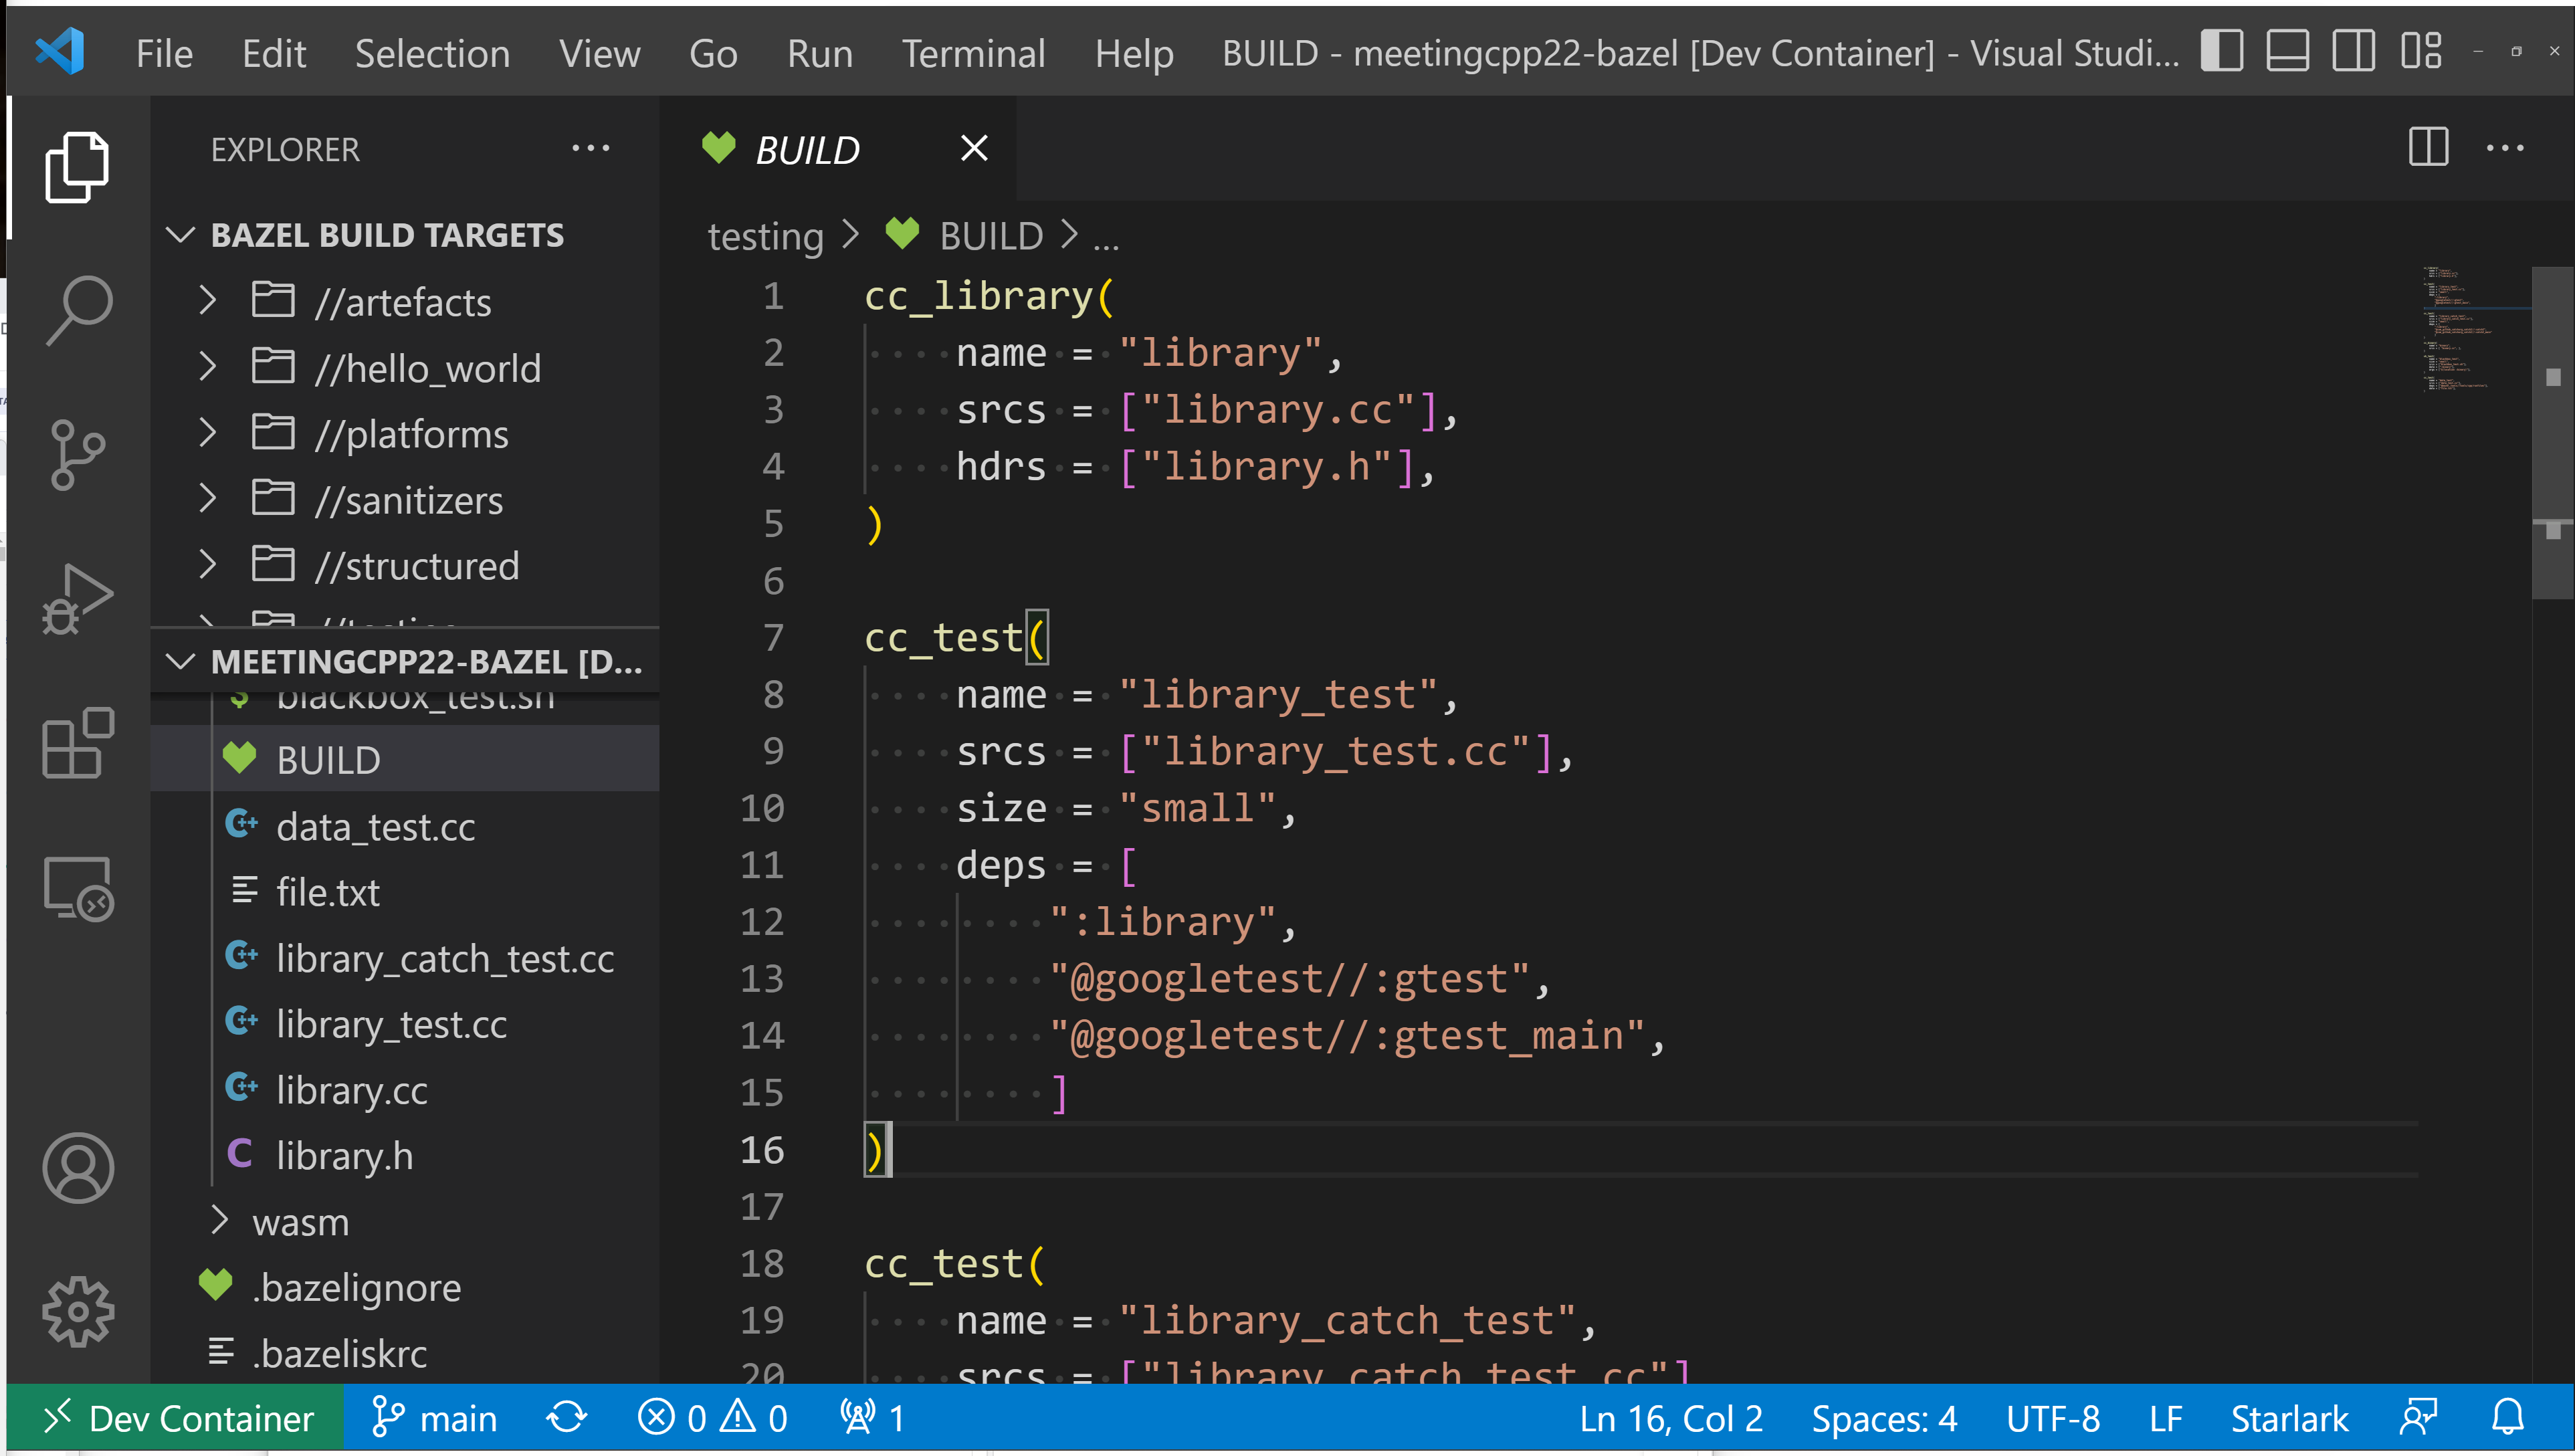
\includegraphics[width=\paperwidth]{slides/static_demos/02_03_BUILD_google.png}}
\begin{frame}[plain]
\end{frame}
}

{
\usebackgroundtemplate{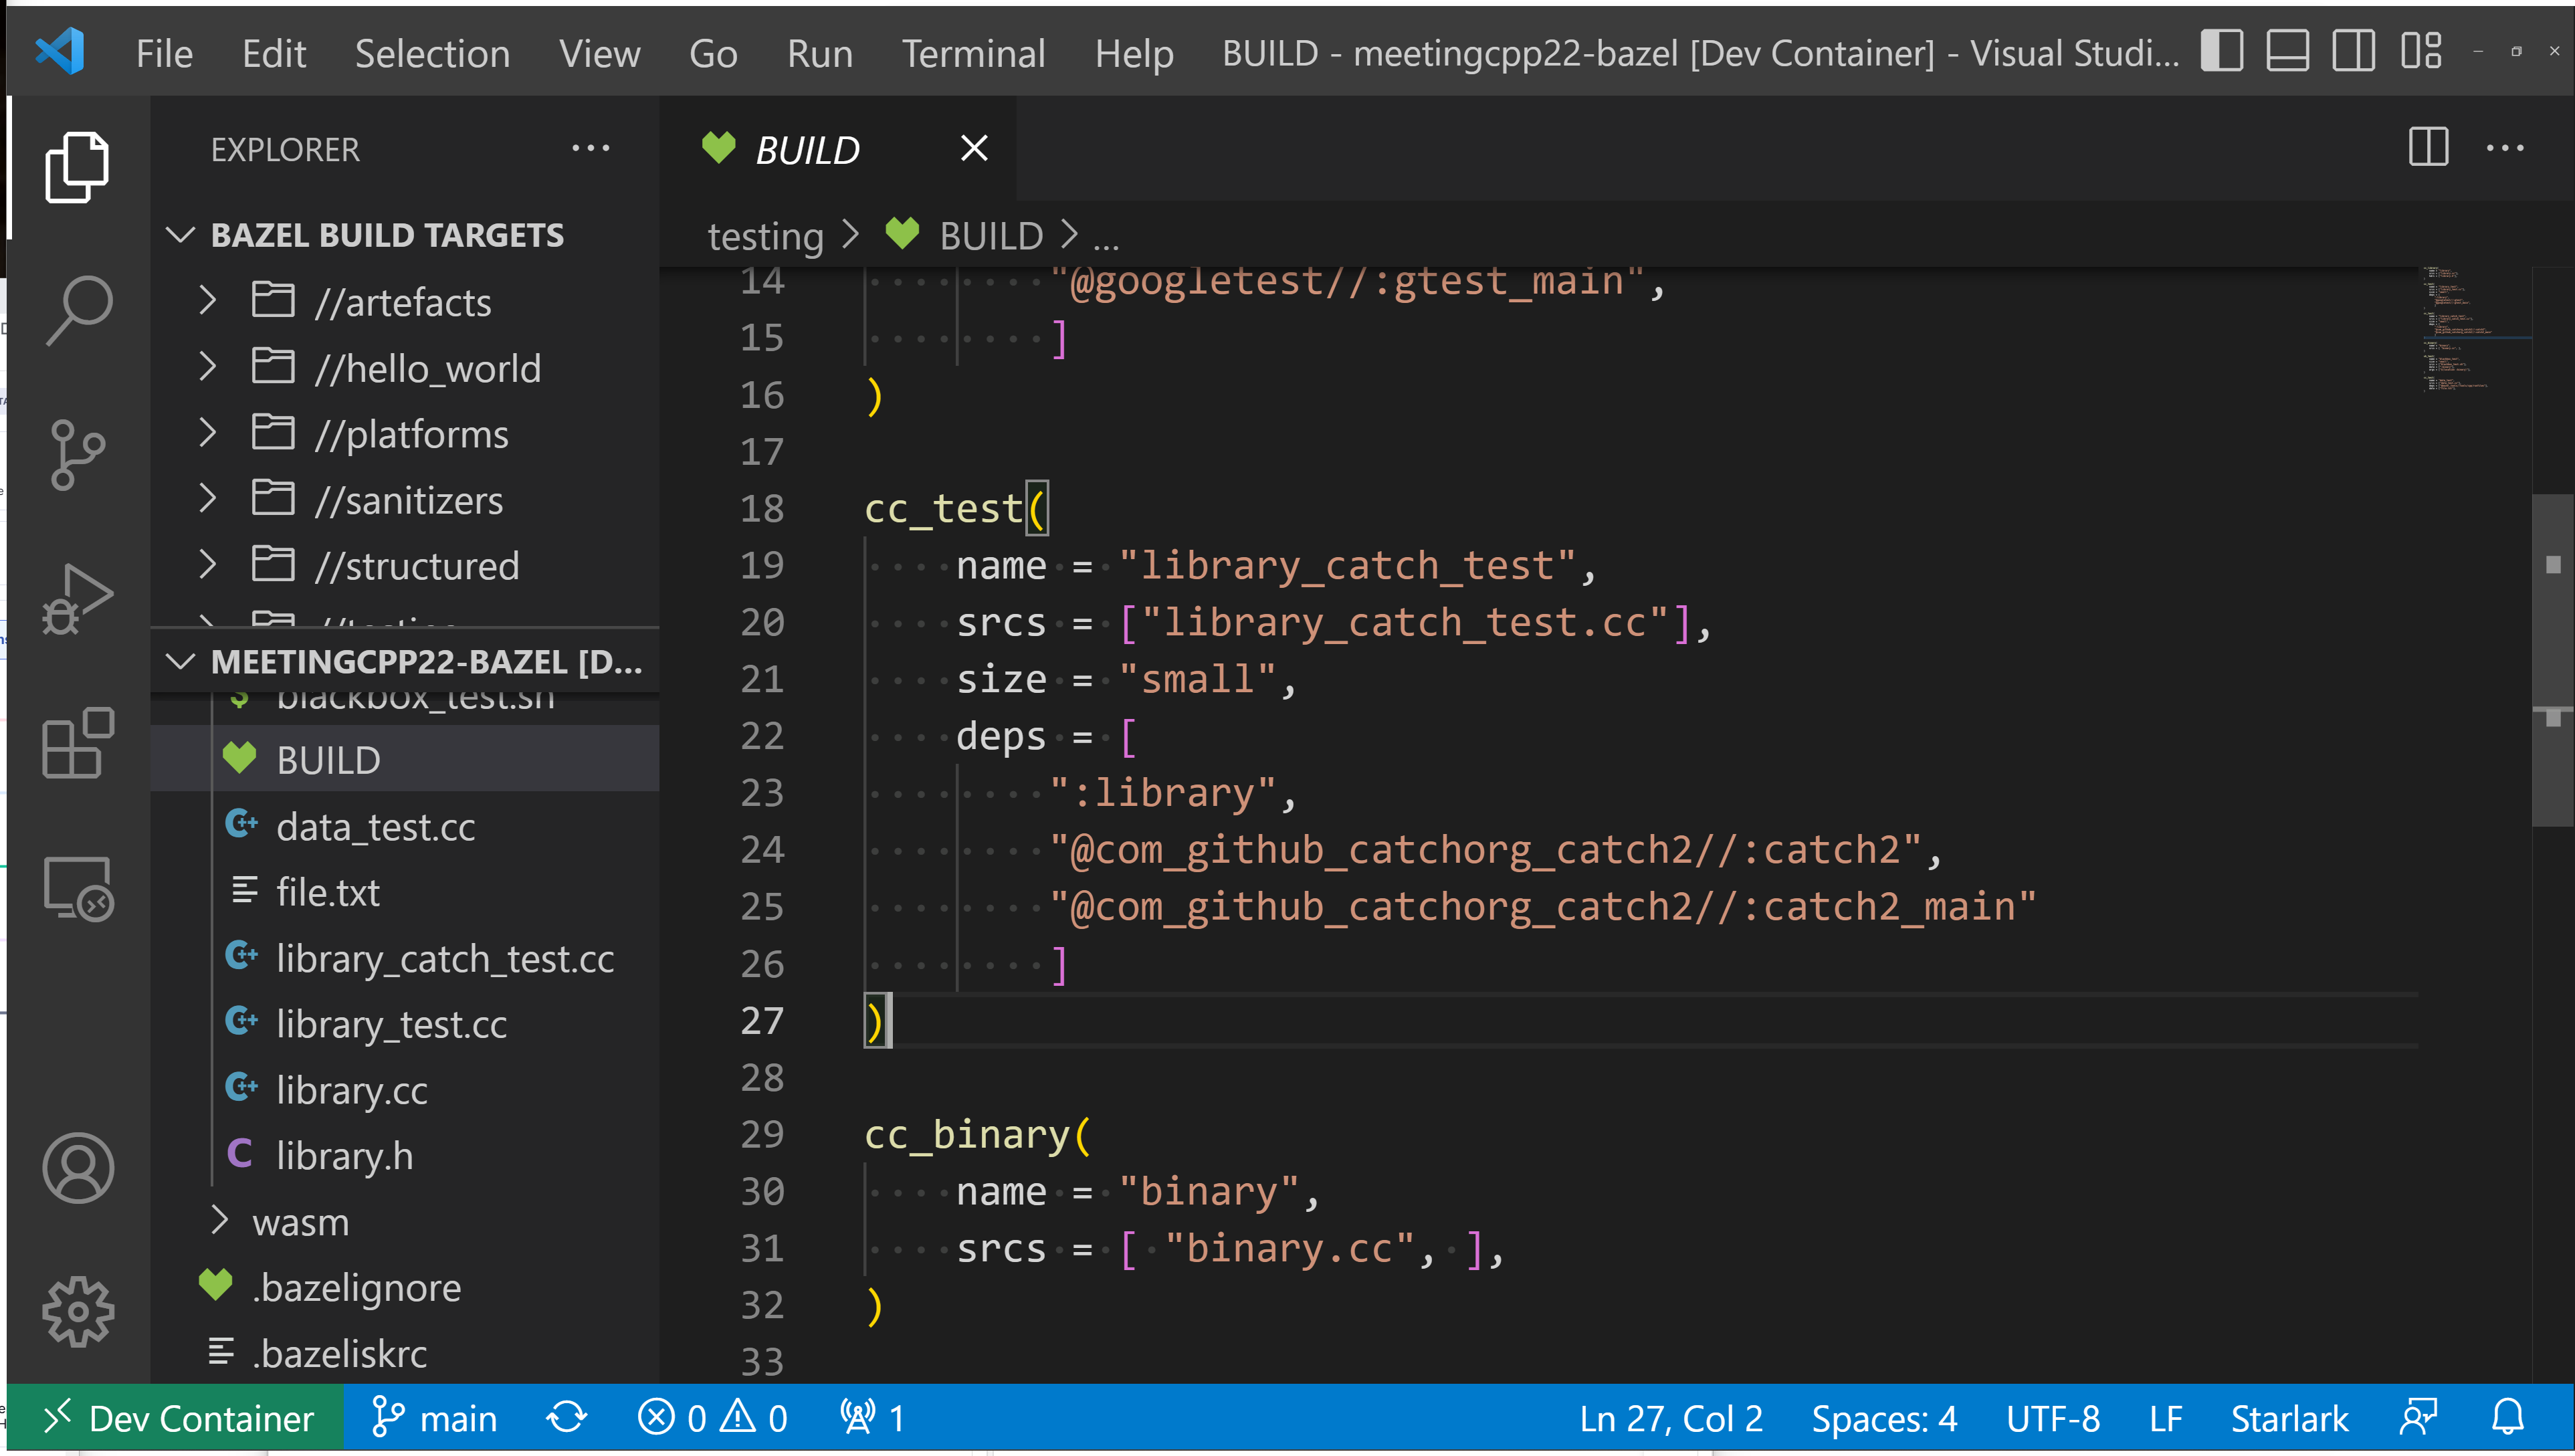
\includegraphics[width=\paperwidth]{slides/static_demos/02_04_BUILD_catch.png}}
\begin{frame}[plain]
\end{frame}
}

{
\usebackgroundtemplate{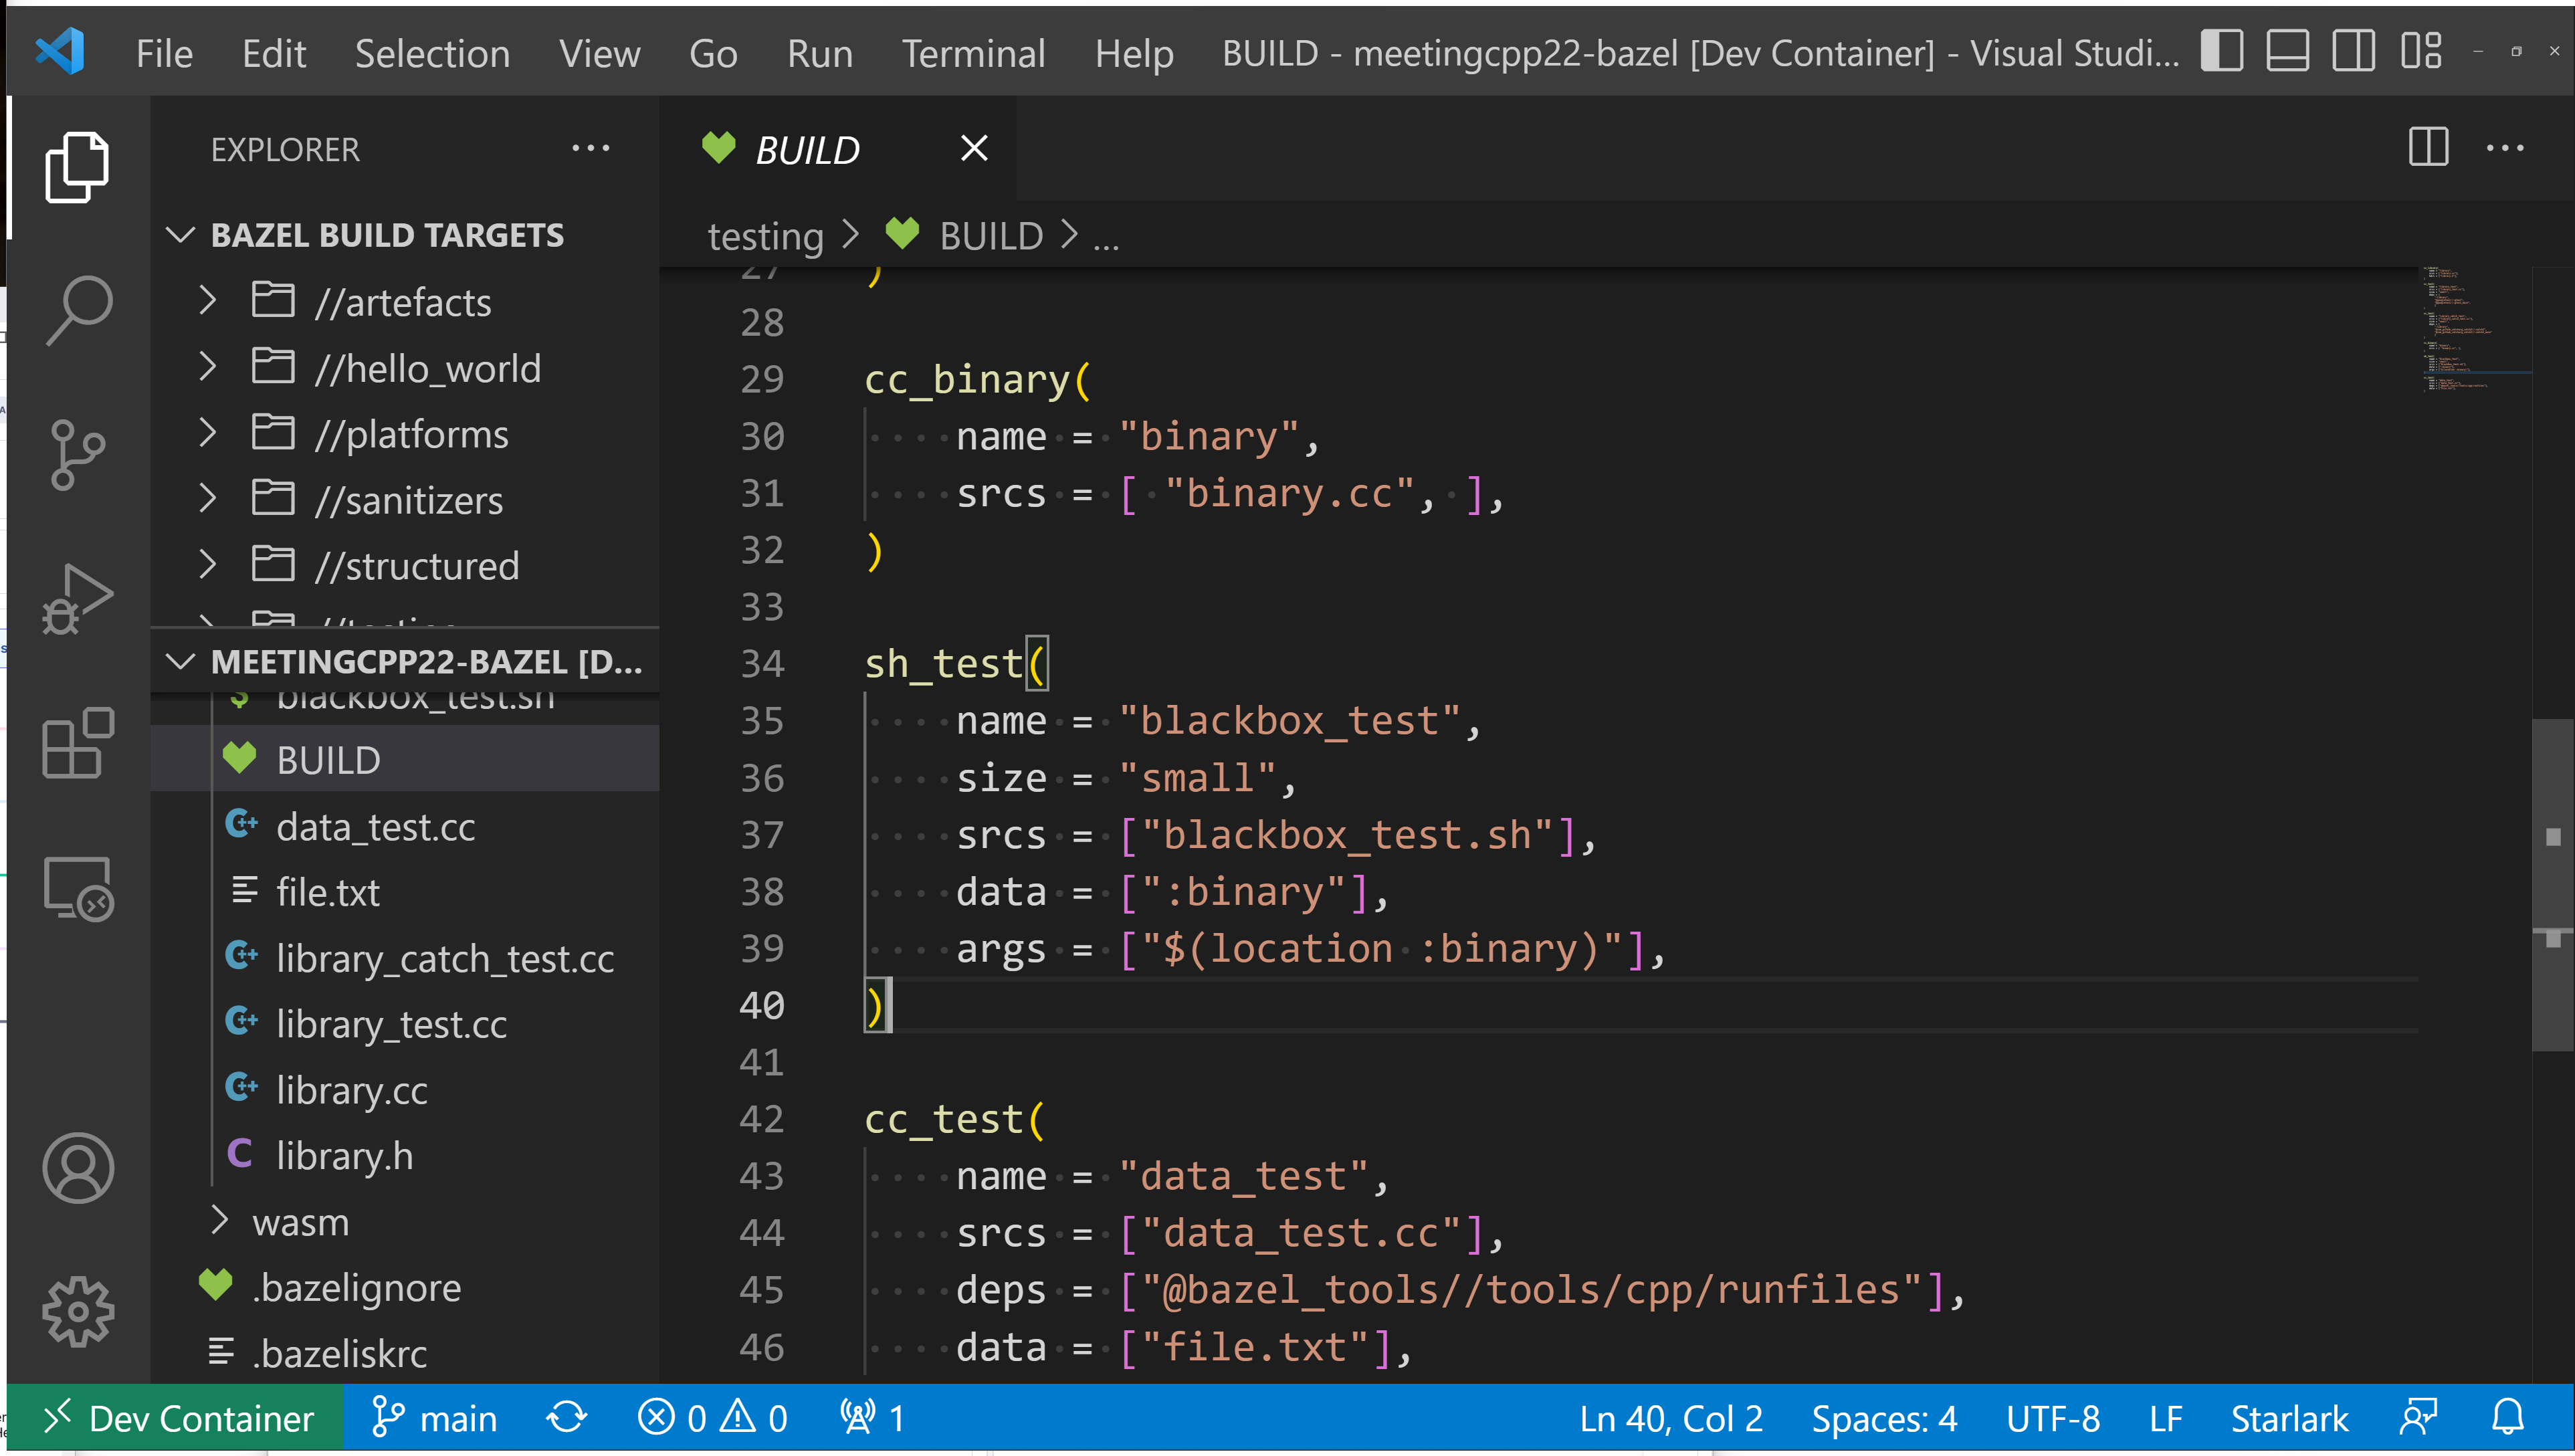
\includegraphics[width=\paperwidth]{slides/static_demos/02_05_blackbox.png}}
\begin{frame}[plain]
\end{frame}
}

{
\usebackgroundtemplate{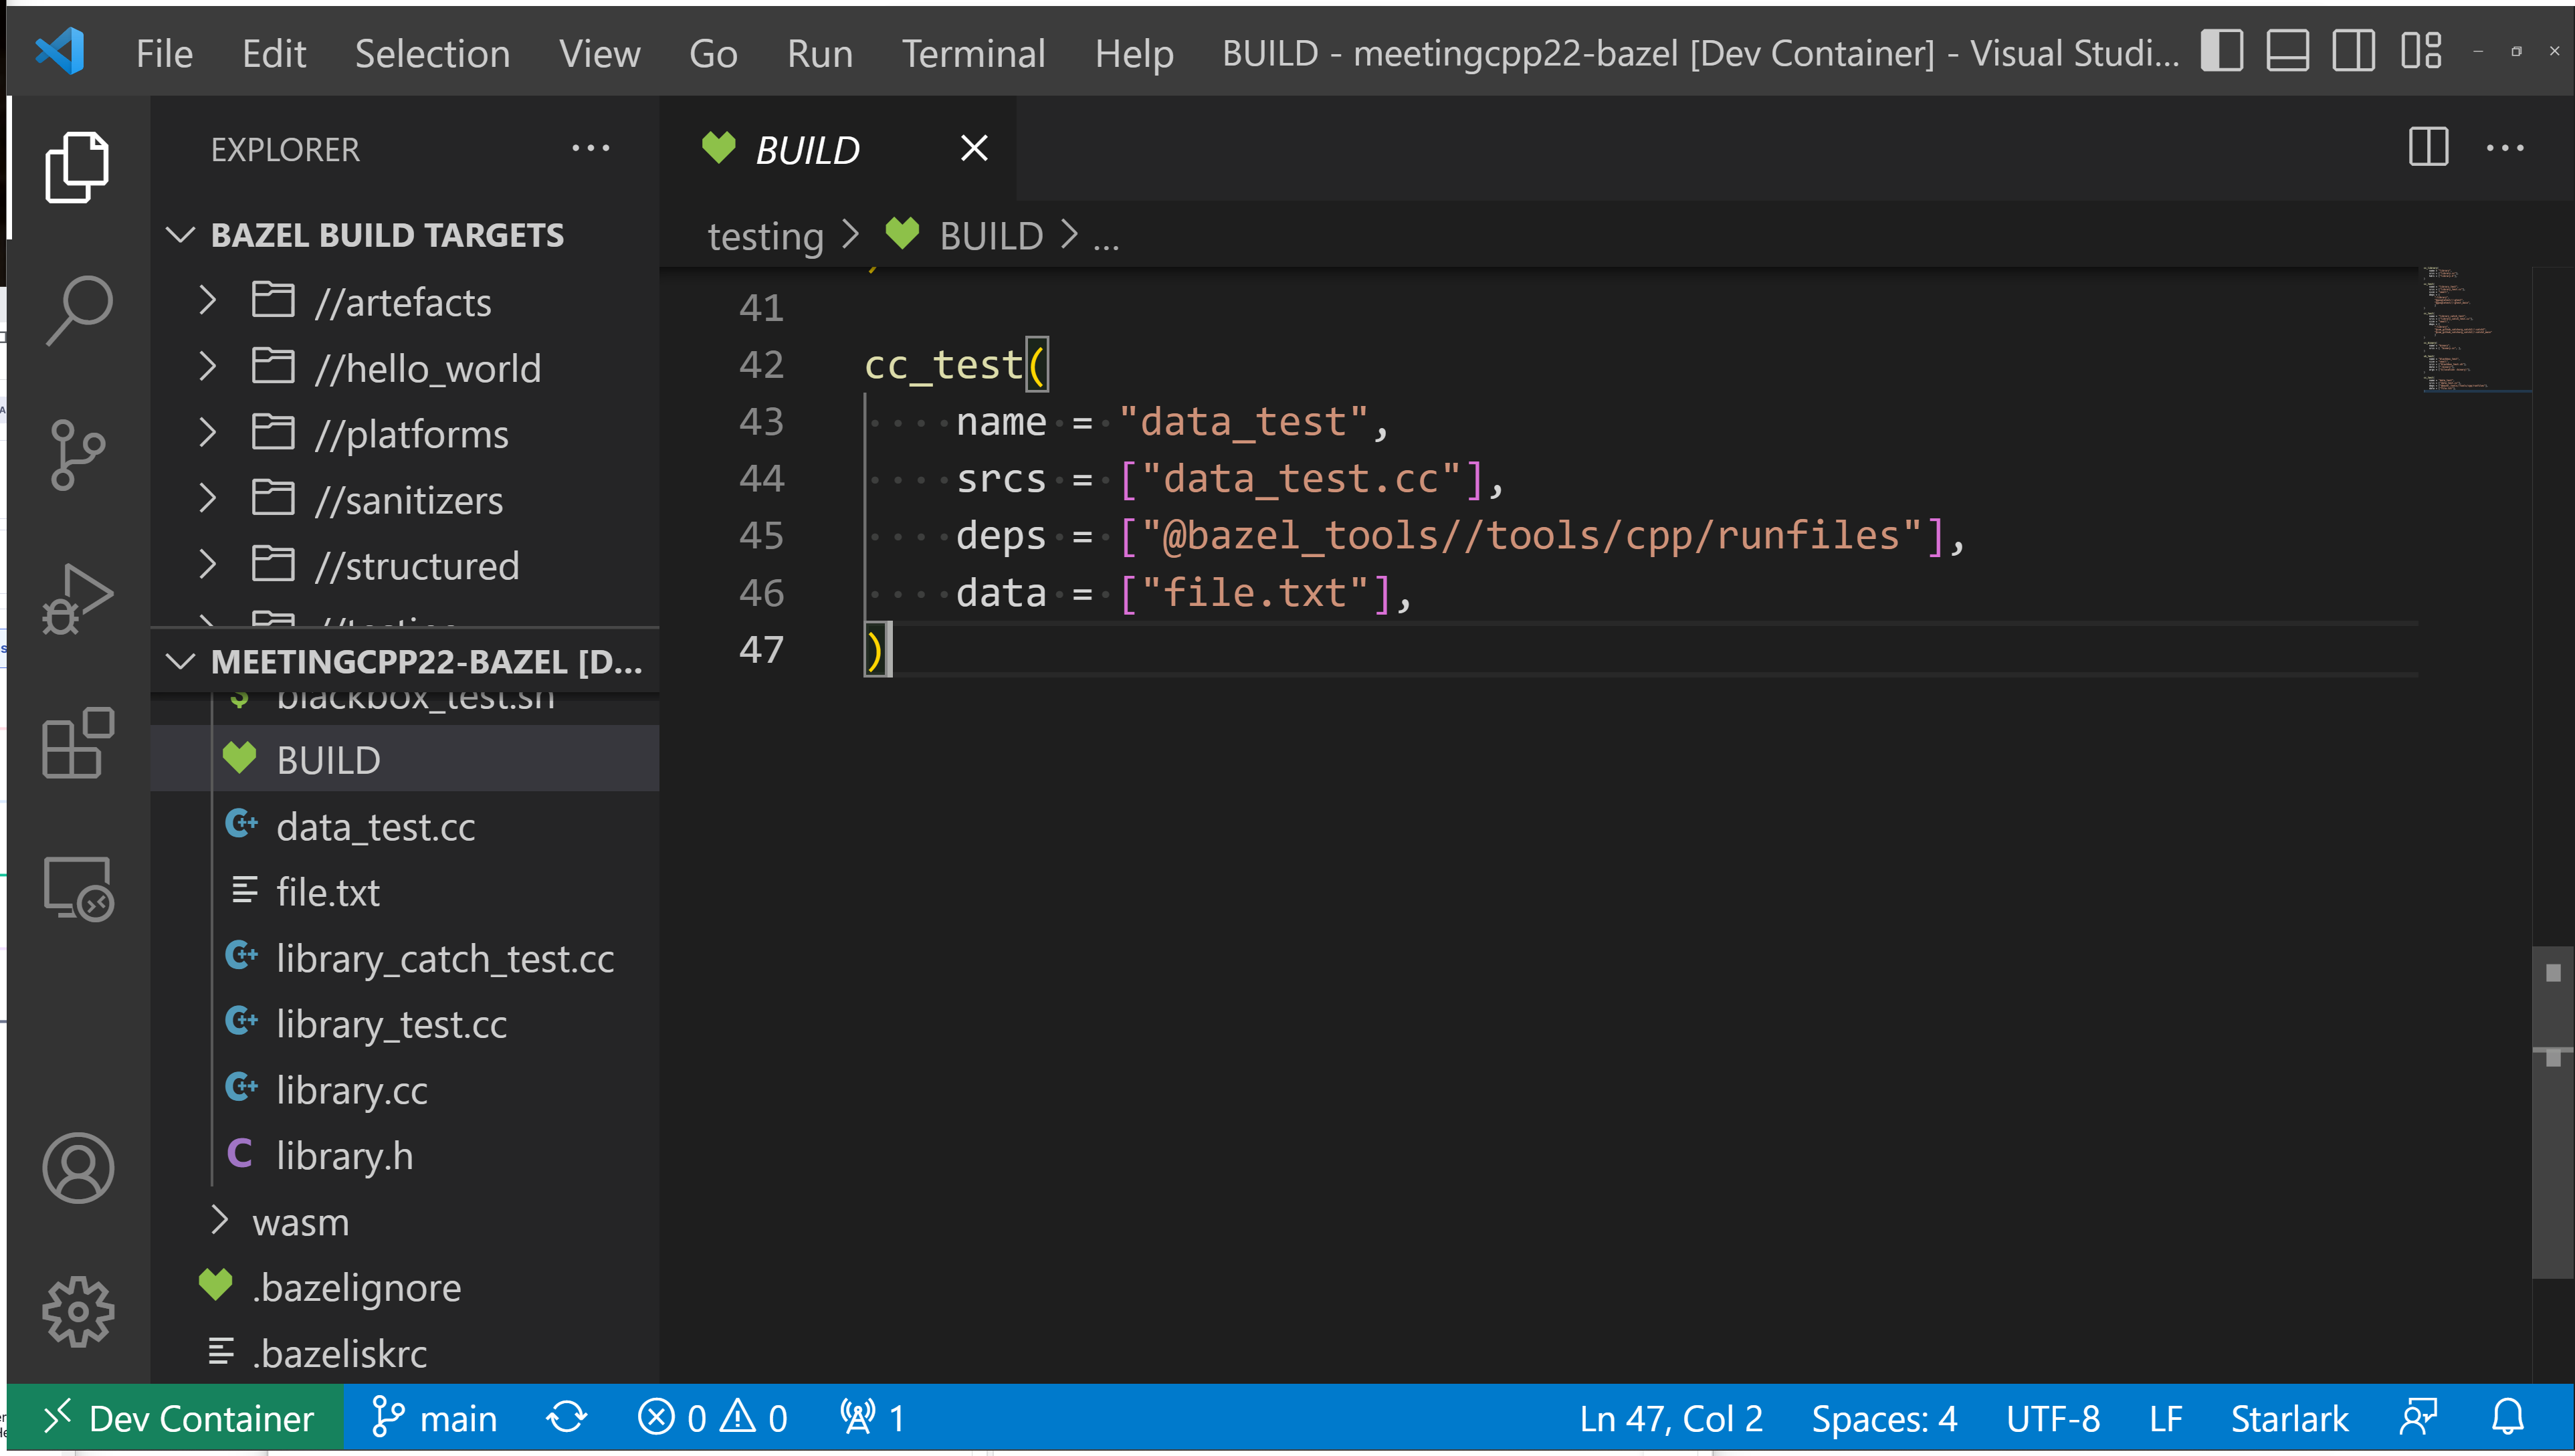
\includegraphics[width=\paperwidth]{slides/static_demos/02_06_hermetic.png}}
\begin{frame}[plain]
\end{frame}
}

{
\usebackgroundtemplate{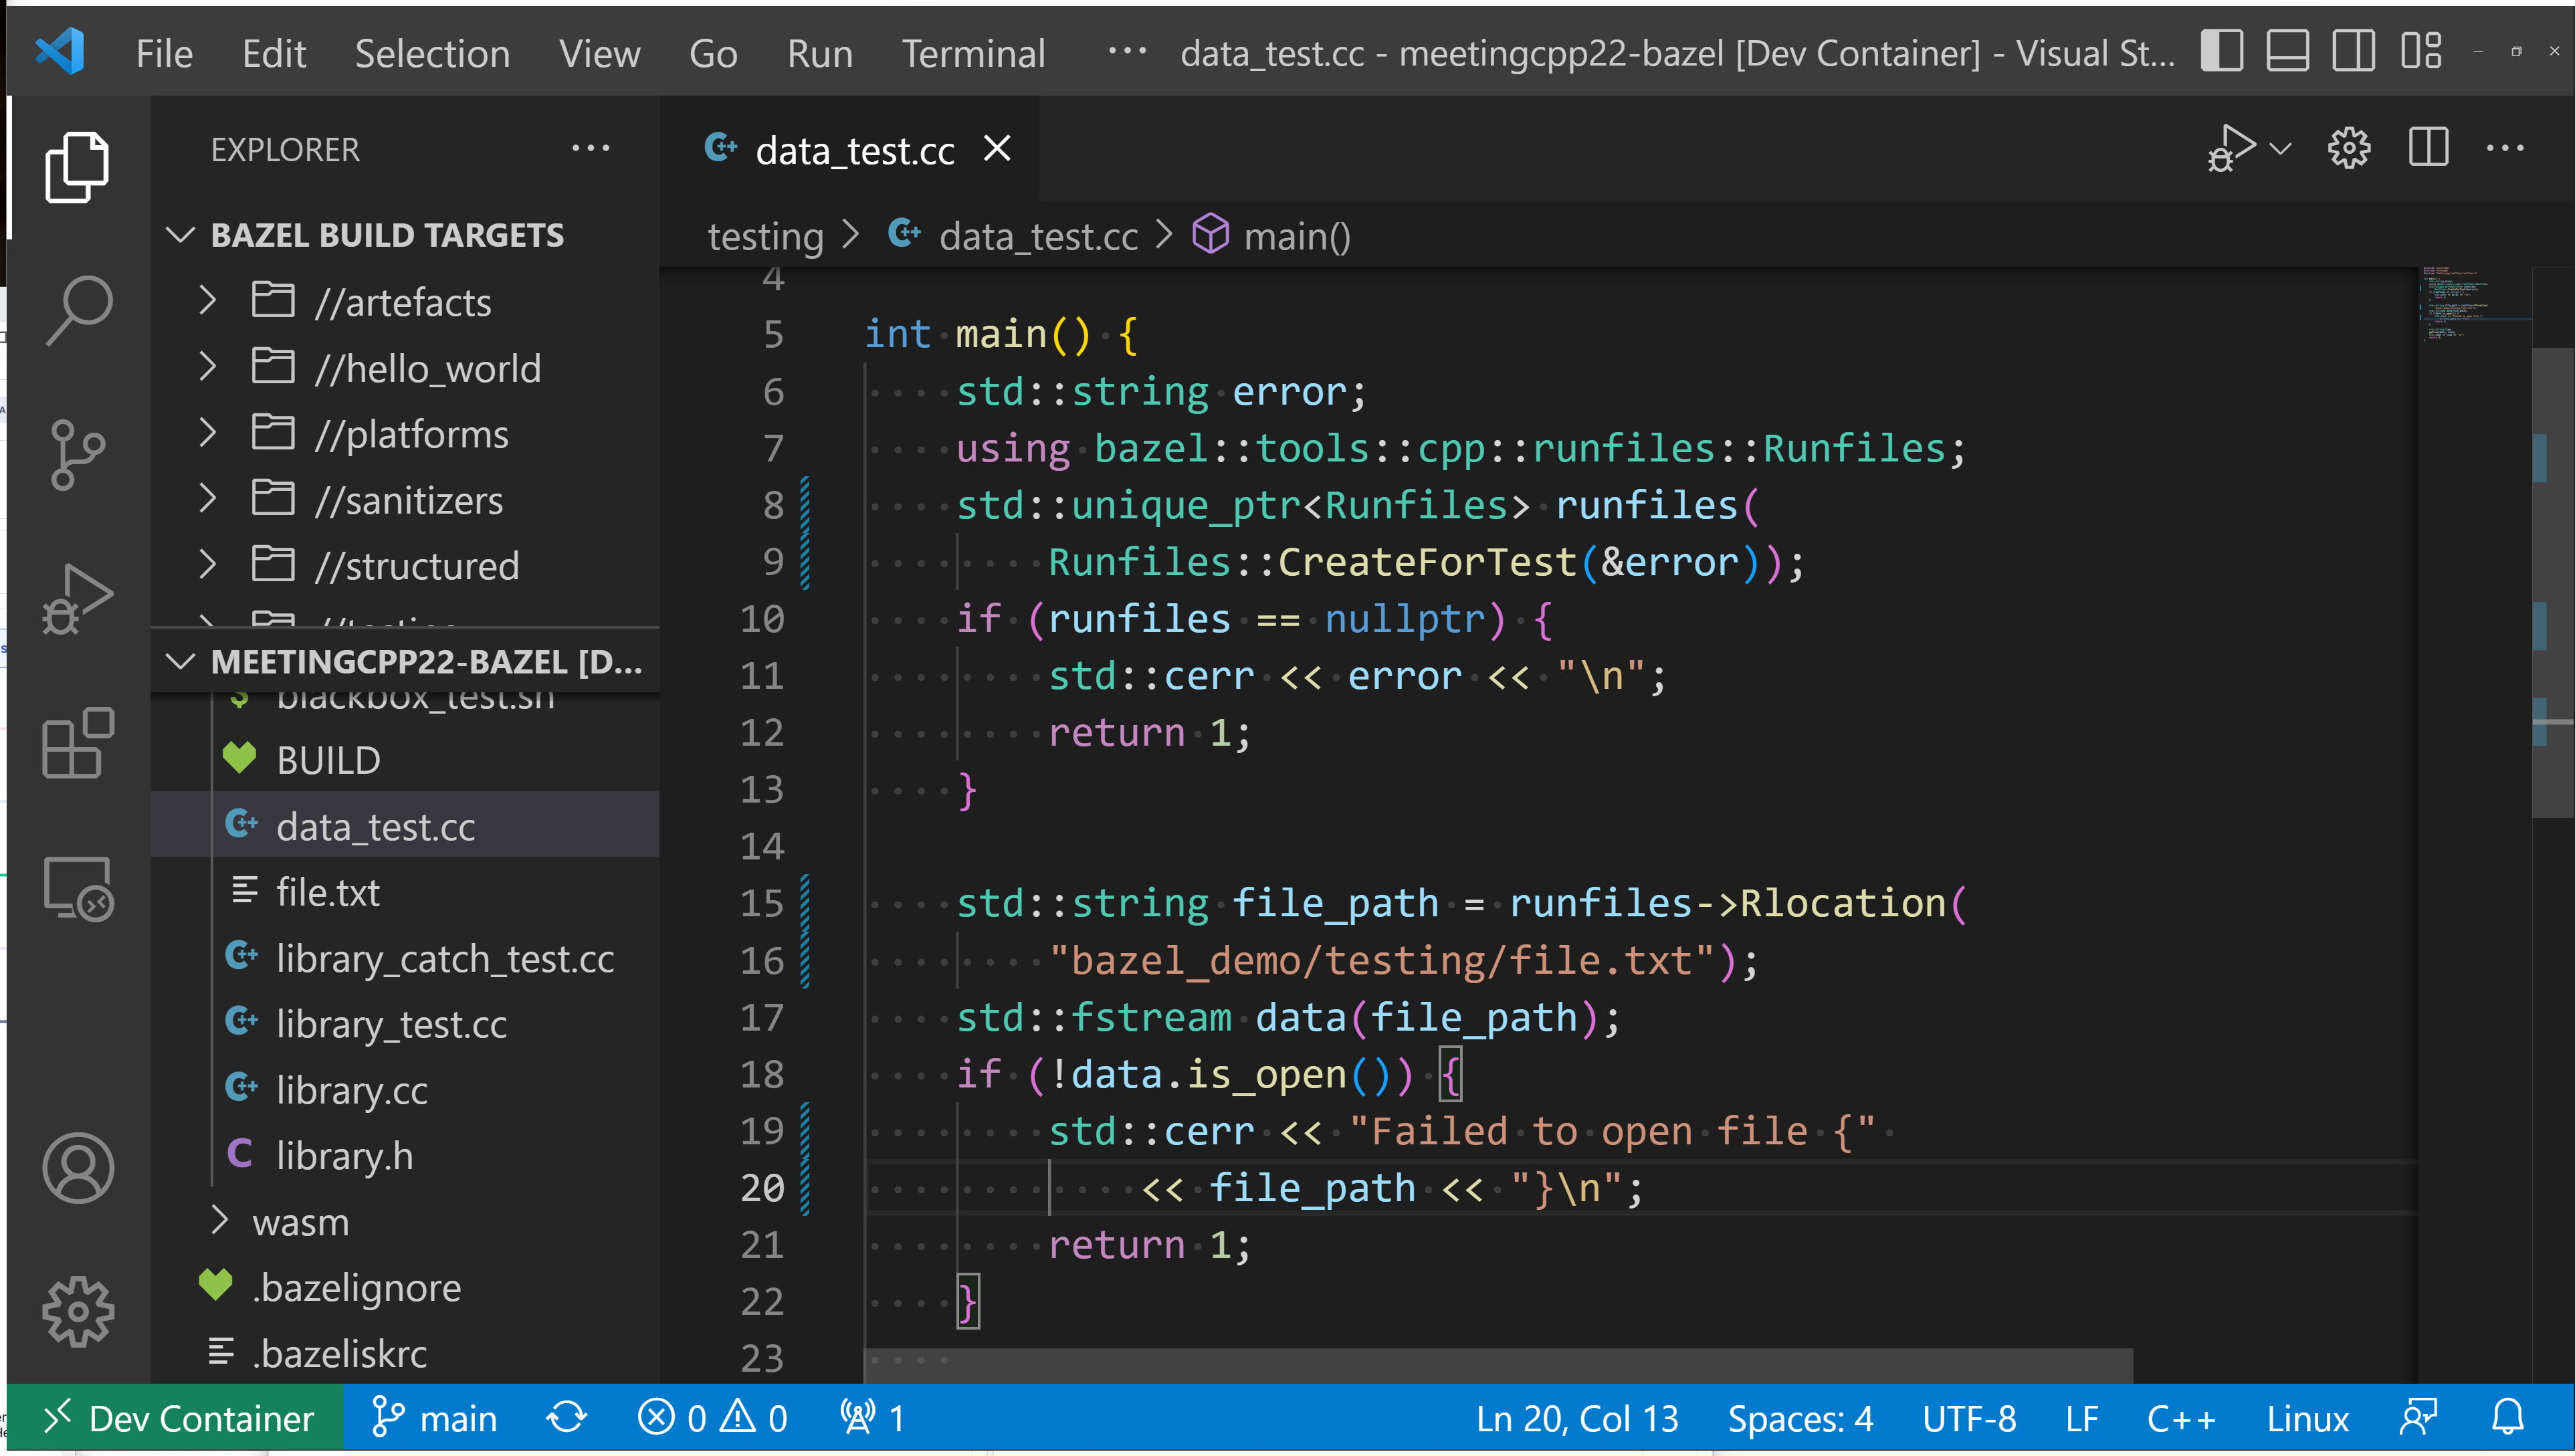
\includegraphics[width=\paperwidth]{slides/static_demos/02_07_library.png}}
\begin{frame}[plain]
\end{frame}
}

{
\usebackgroundtemplate{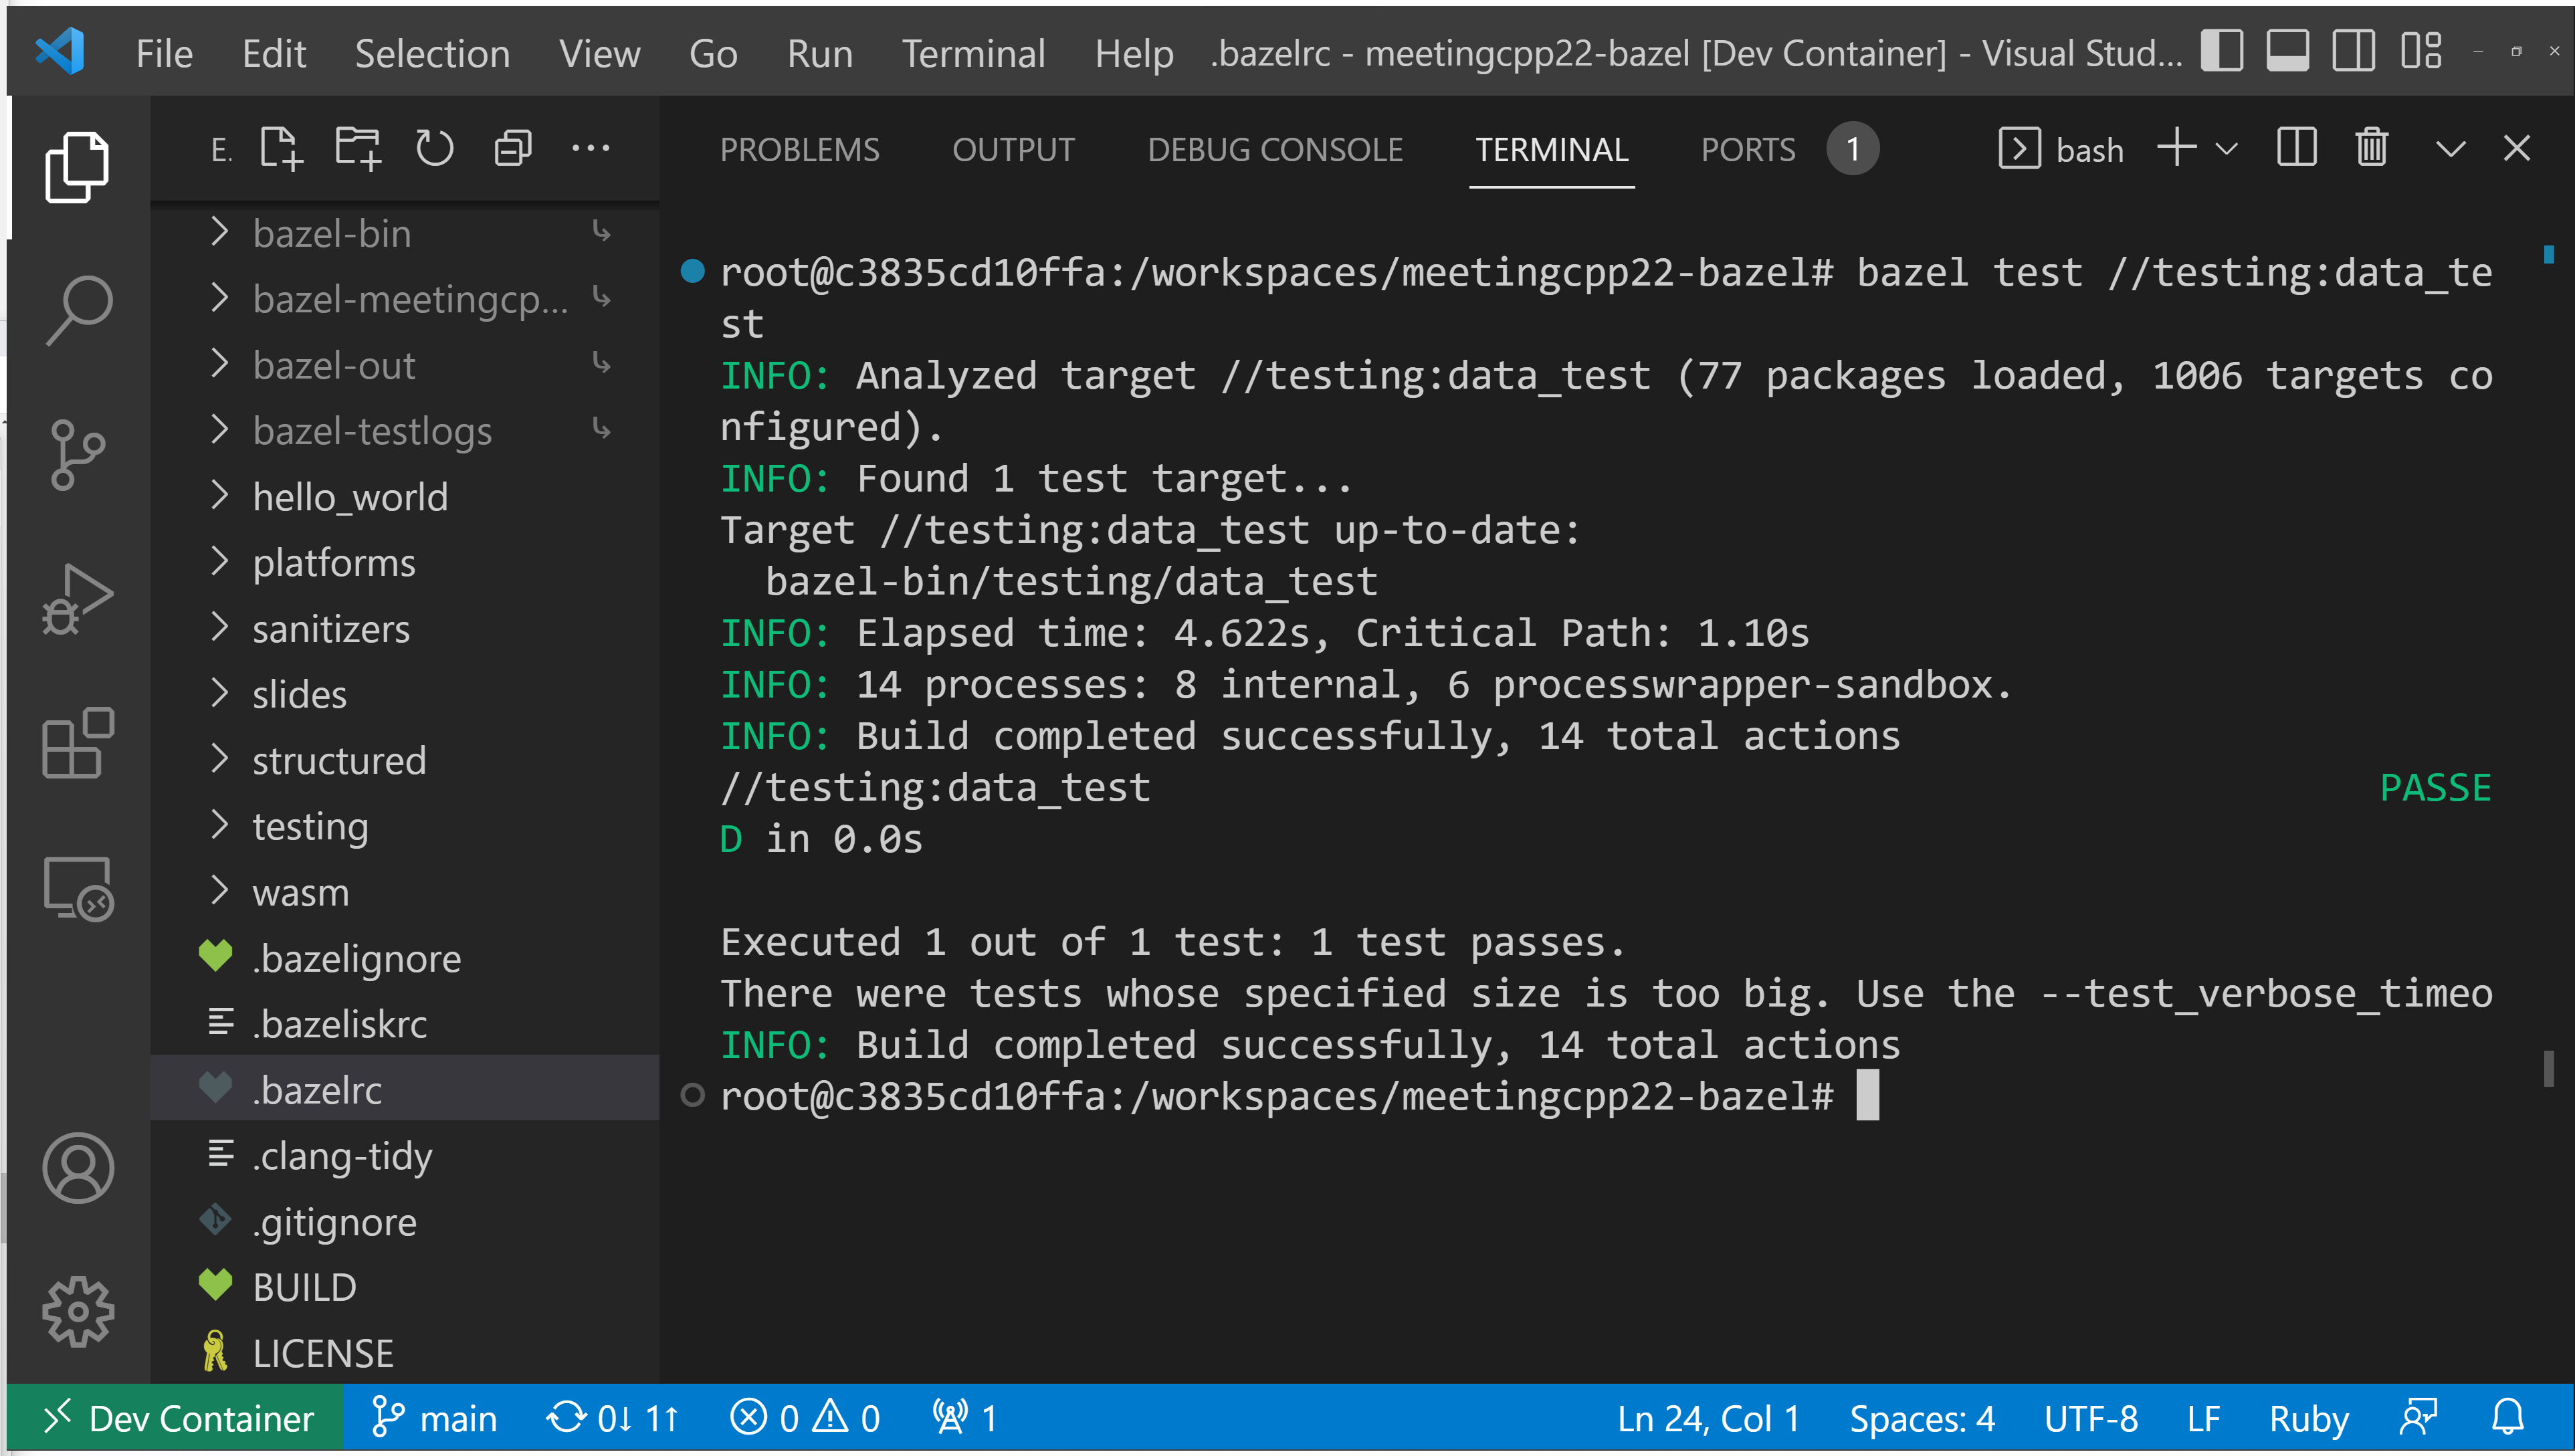
\includegraphics[width=\paperwidth]{slides/static_demos/02_08_test.png}}
\begin{frame}[plain]
\end{frame}
}

{
\usebackgroundtemplate{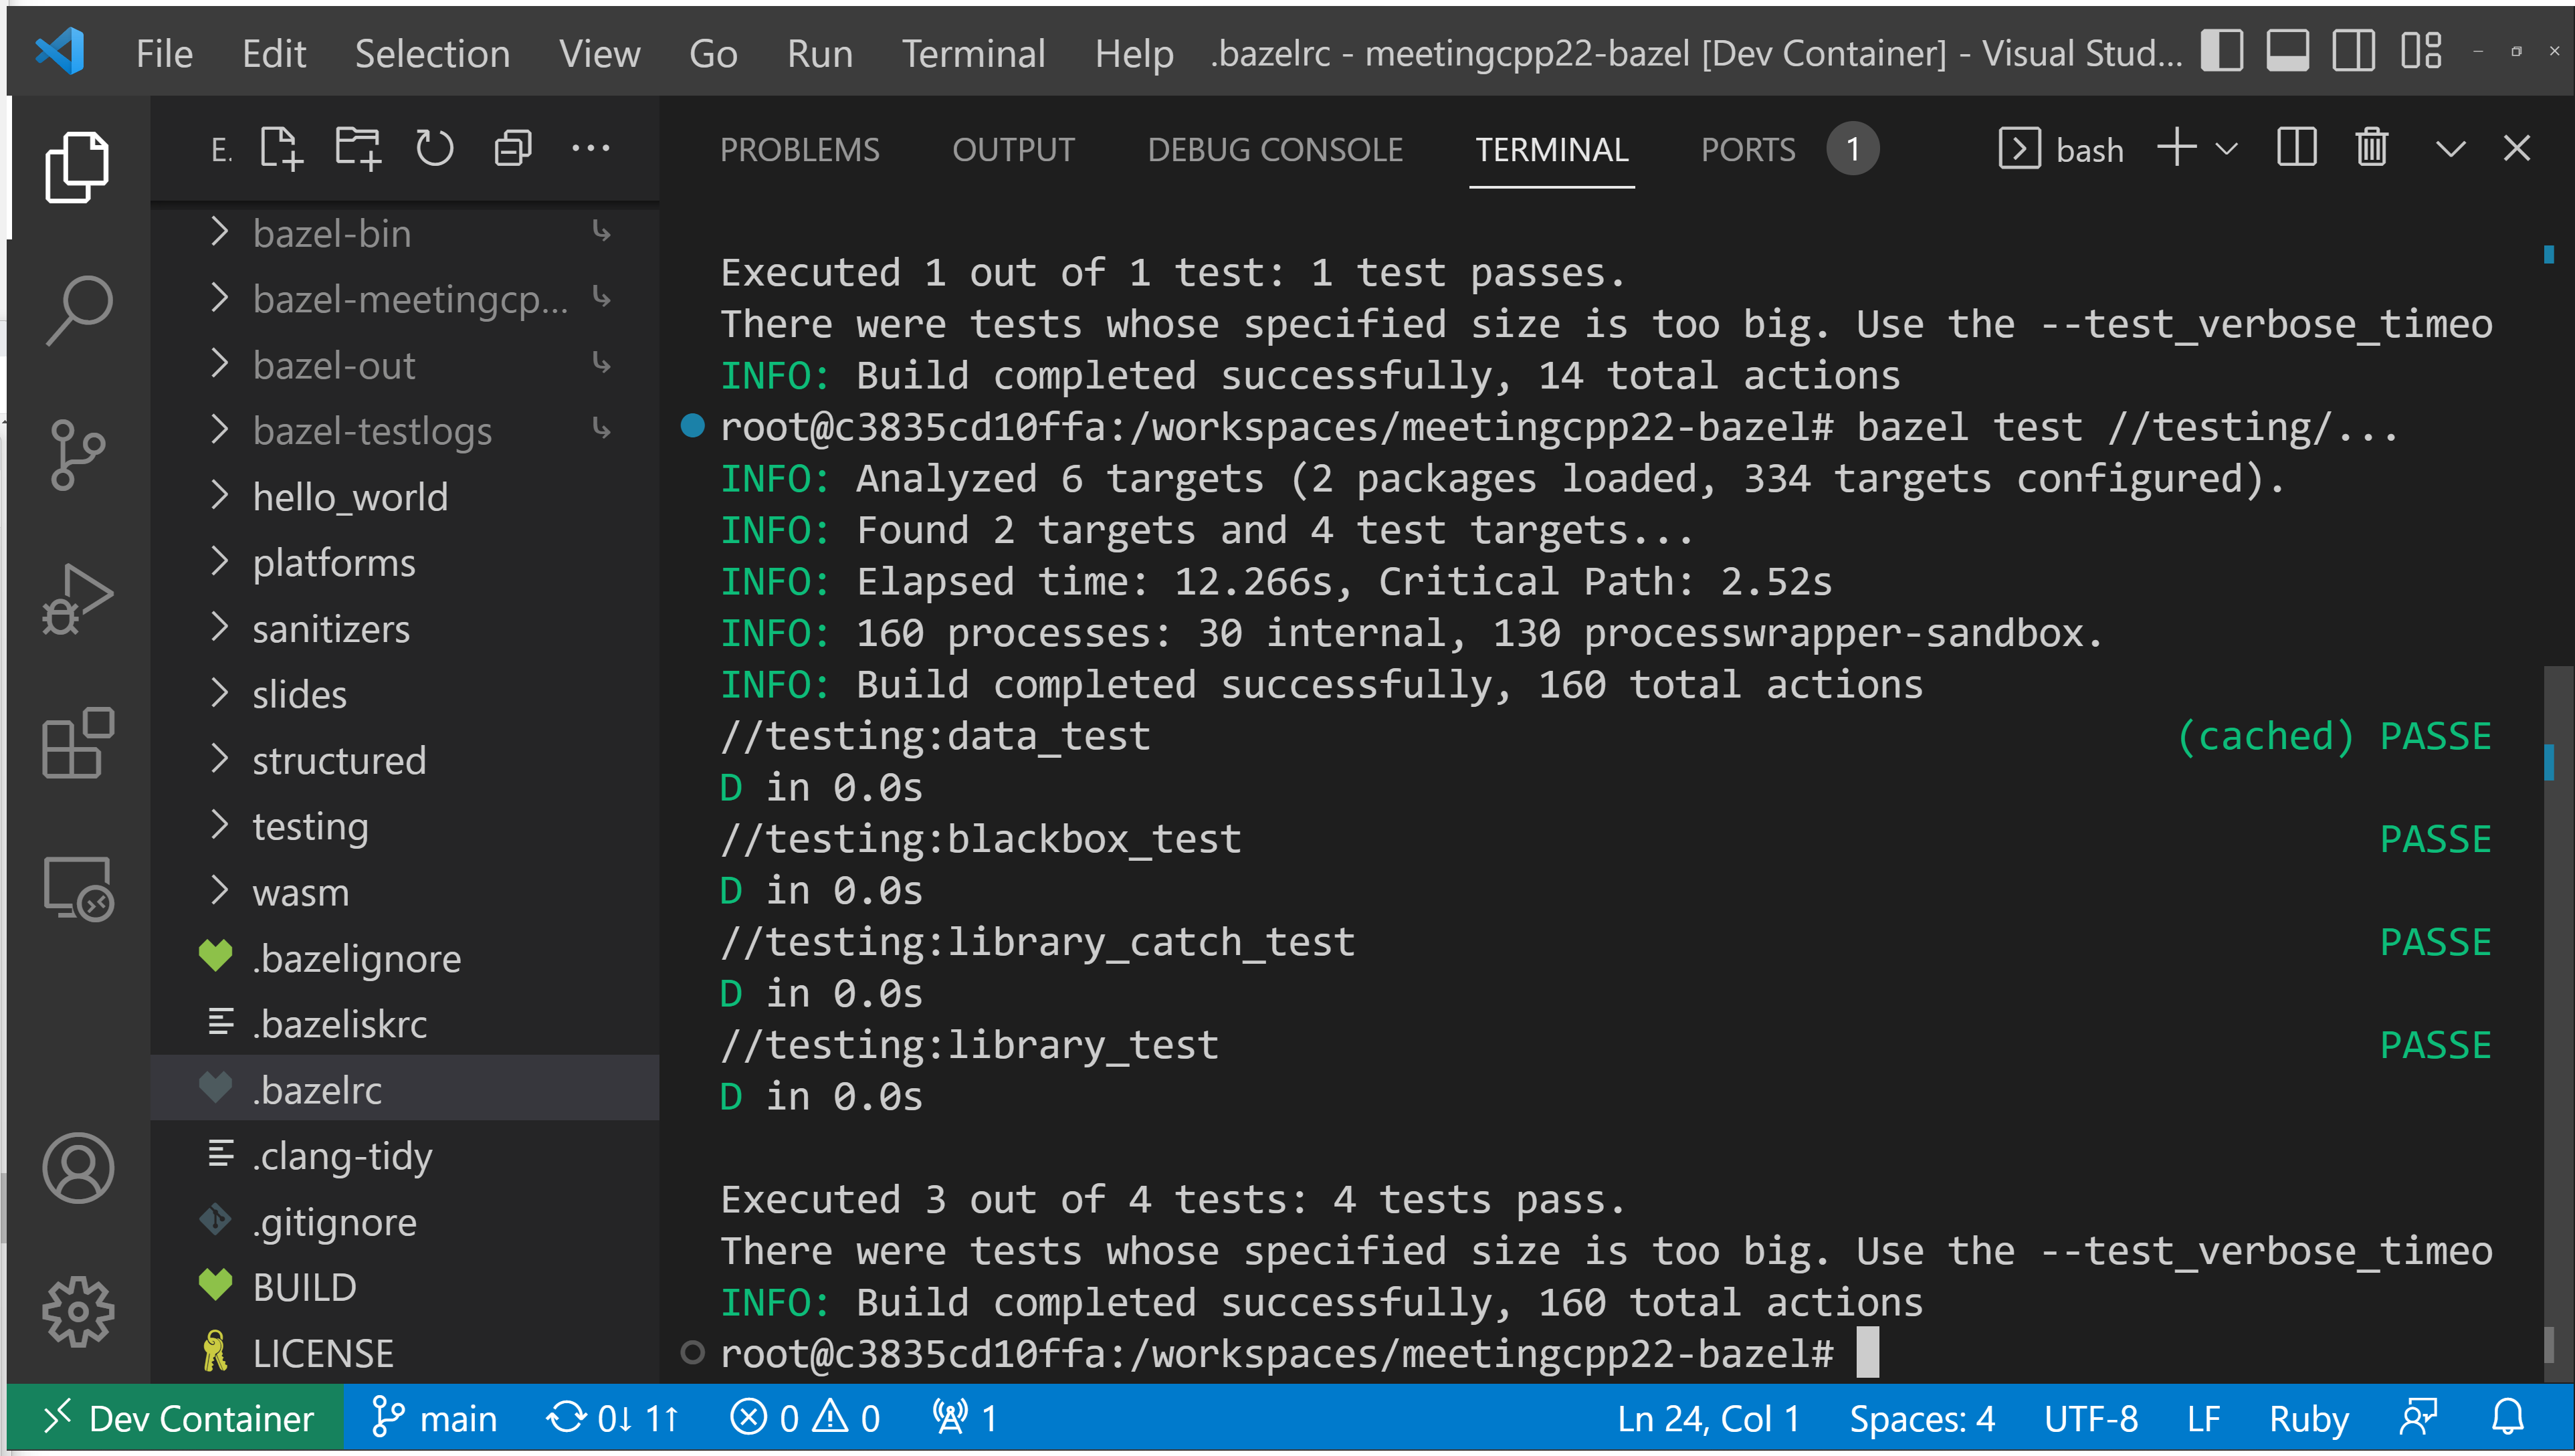
\includegraphics[width=\paperwidth]{slides/static_demos/02_09_test_all.png}}
\begin{frame}[plain]
\end{frame}
}

\begin{frame}{}
    \begin{center}
        \begin{Huge}Sanitizers and Static Analyzers\end{Huge}
    \end{center}
\end{frame}

{
\usebackgroundtemplate{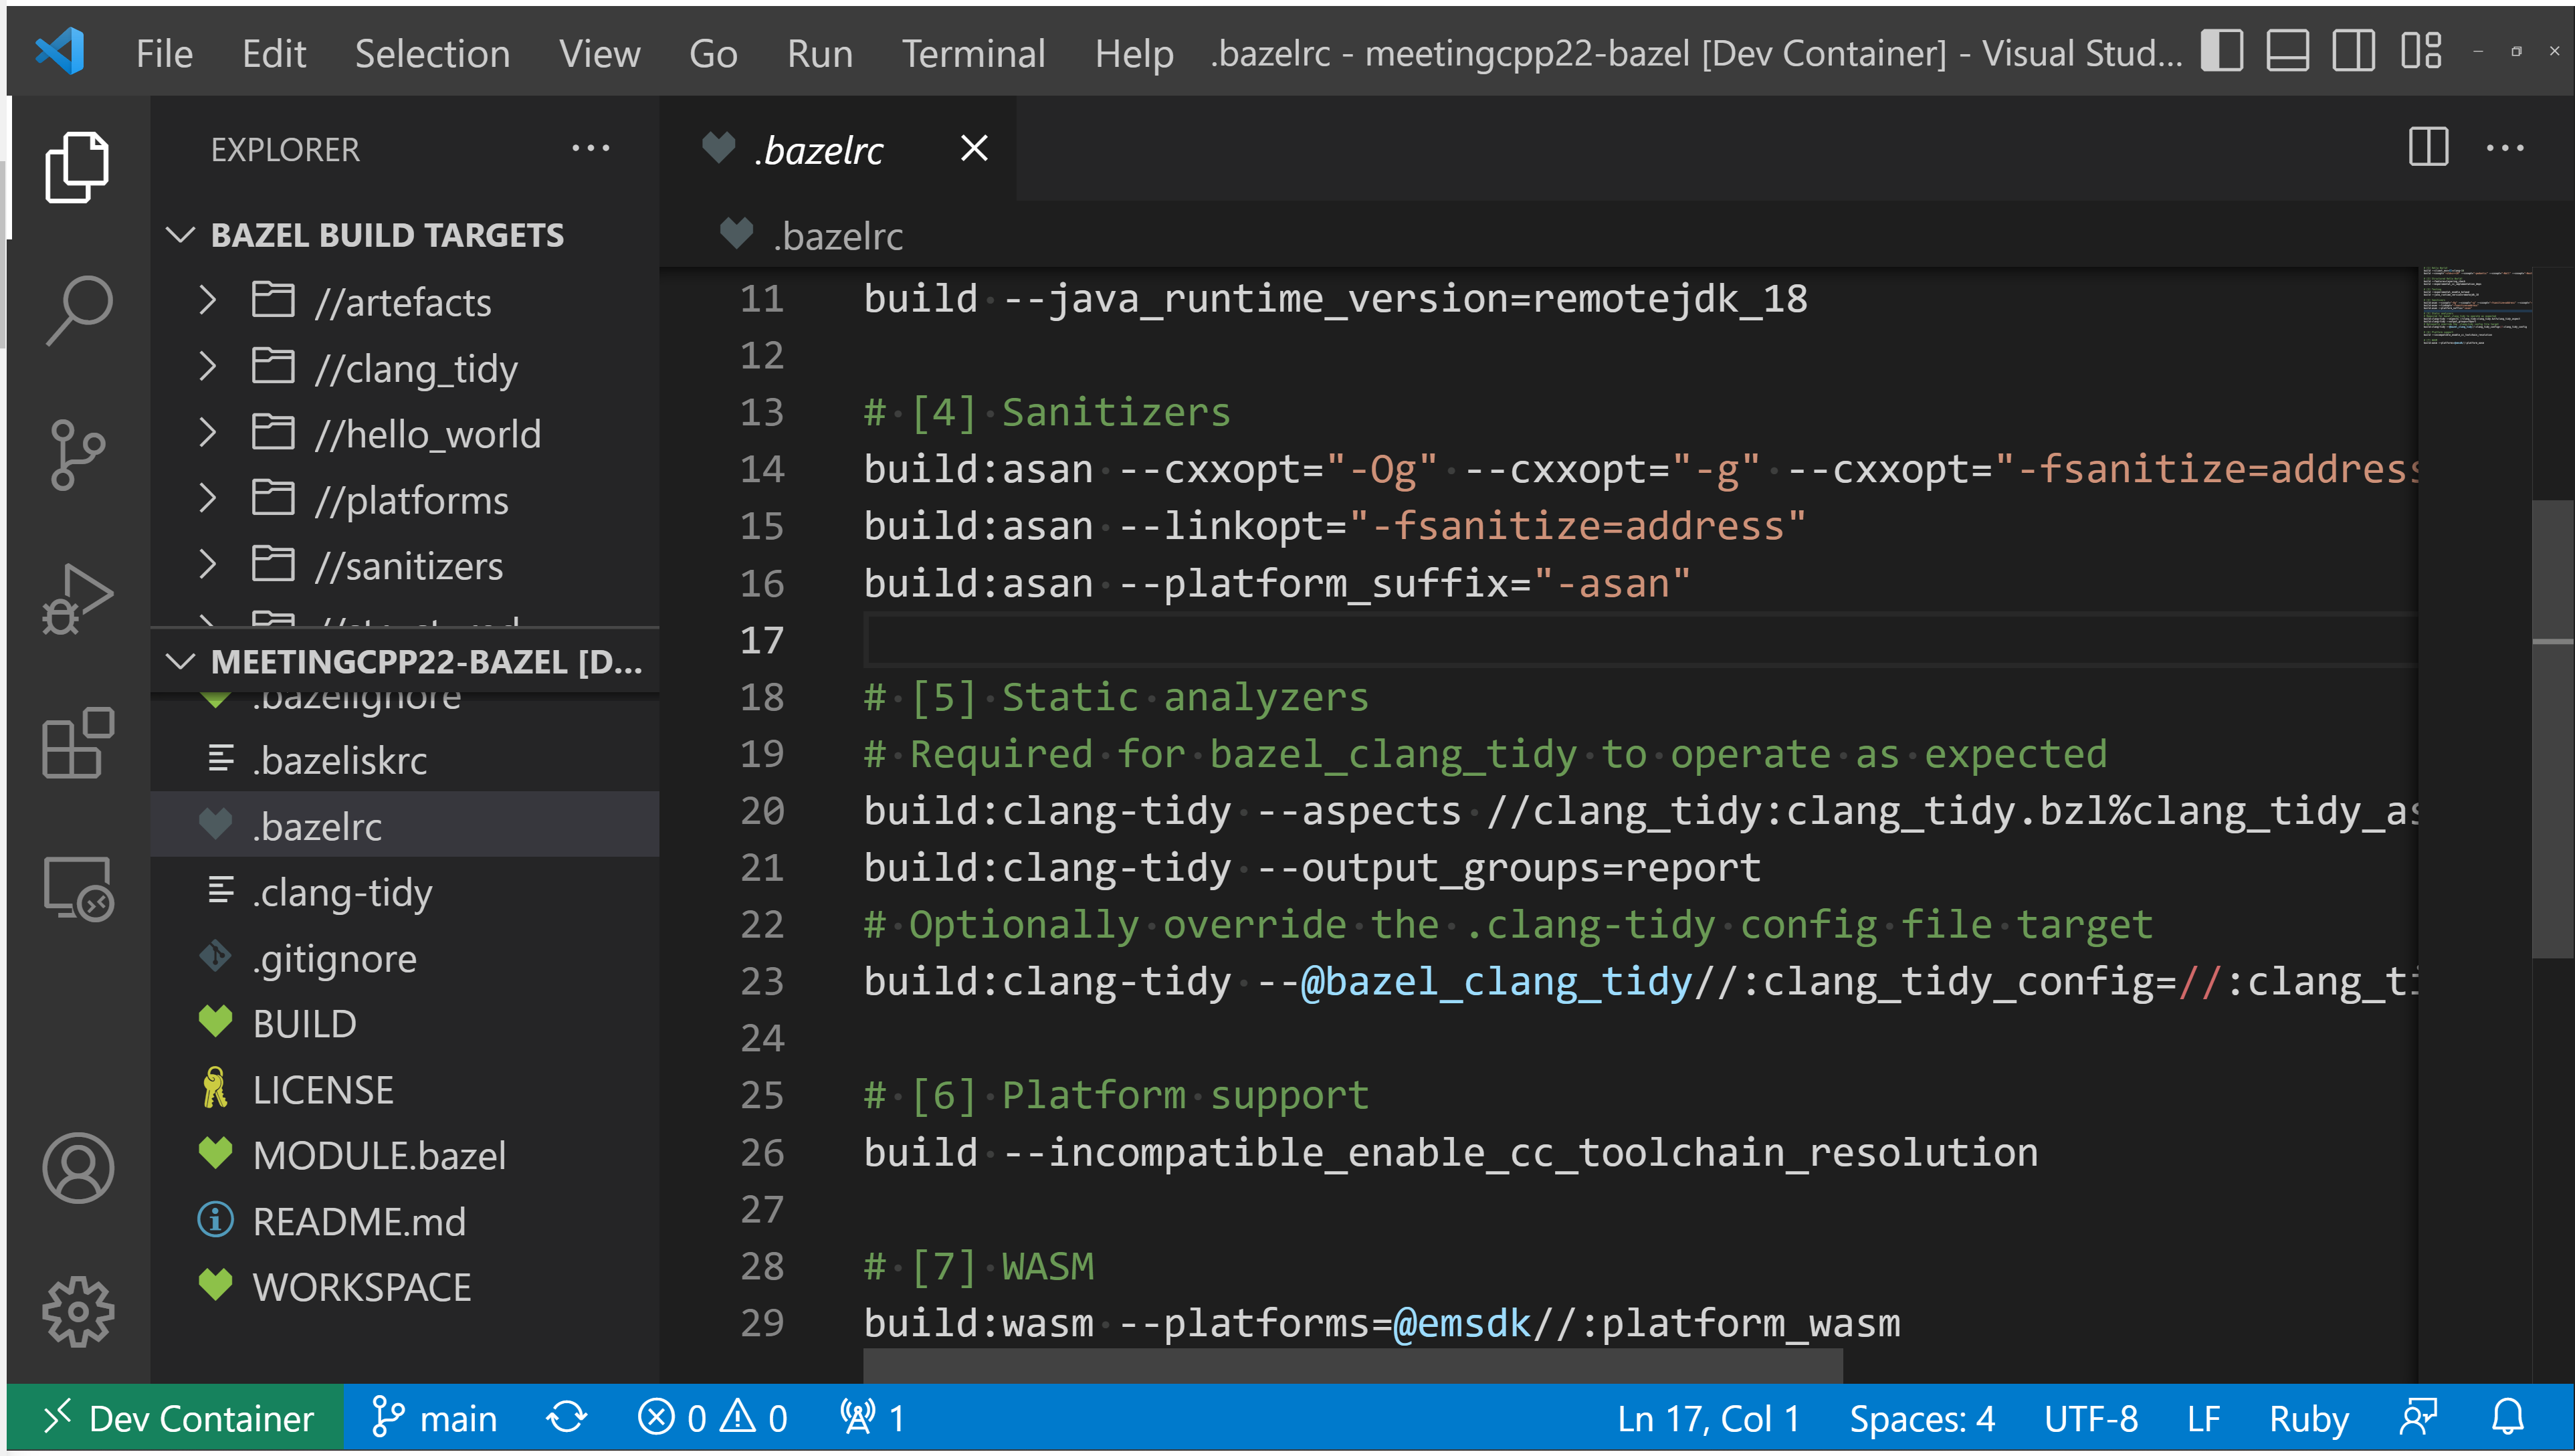
\includegraphics[width=\paperwidth]{slides/static_demos/03_00_bazelrc.png}}
\begin{frame}[plain]
\end{frame}
}

{
\usebackgroundtemplate{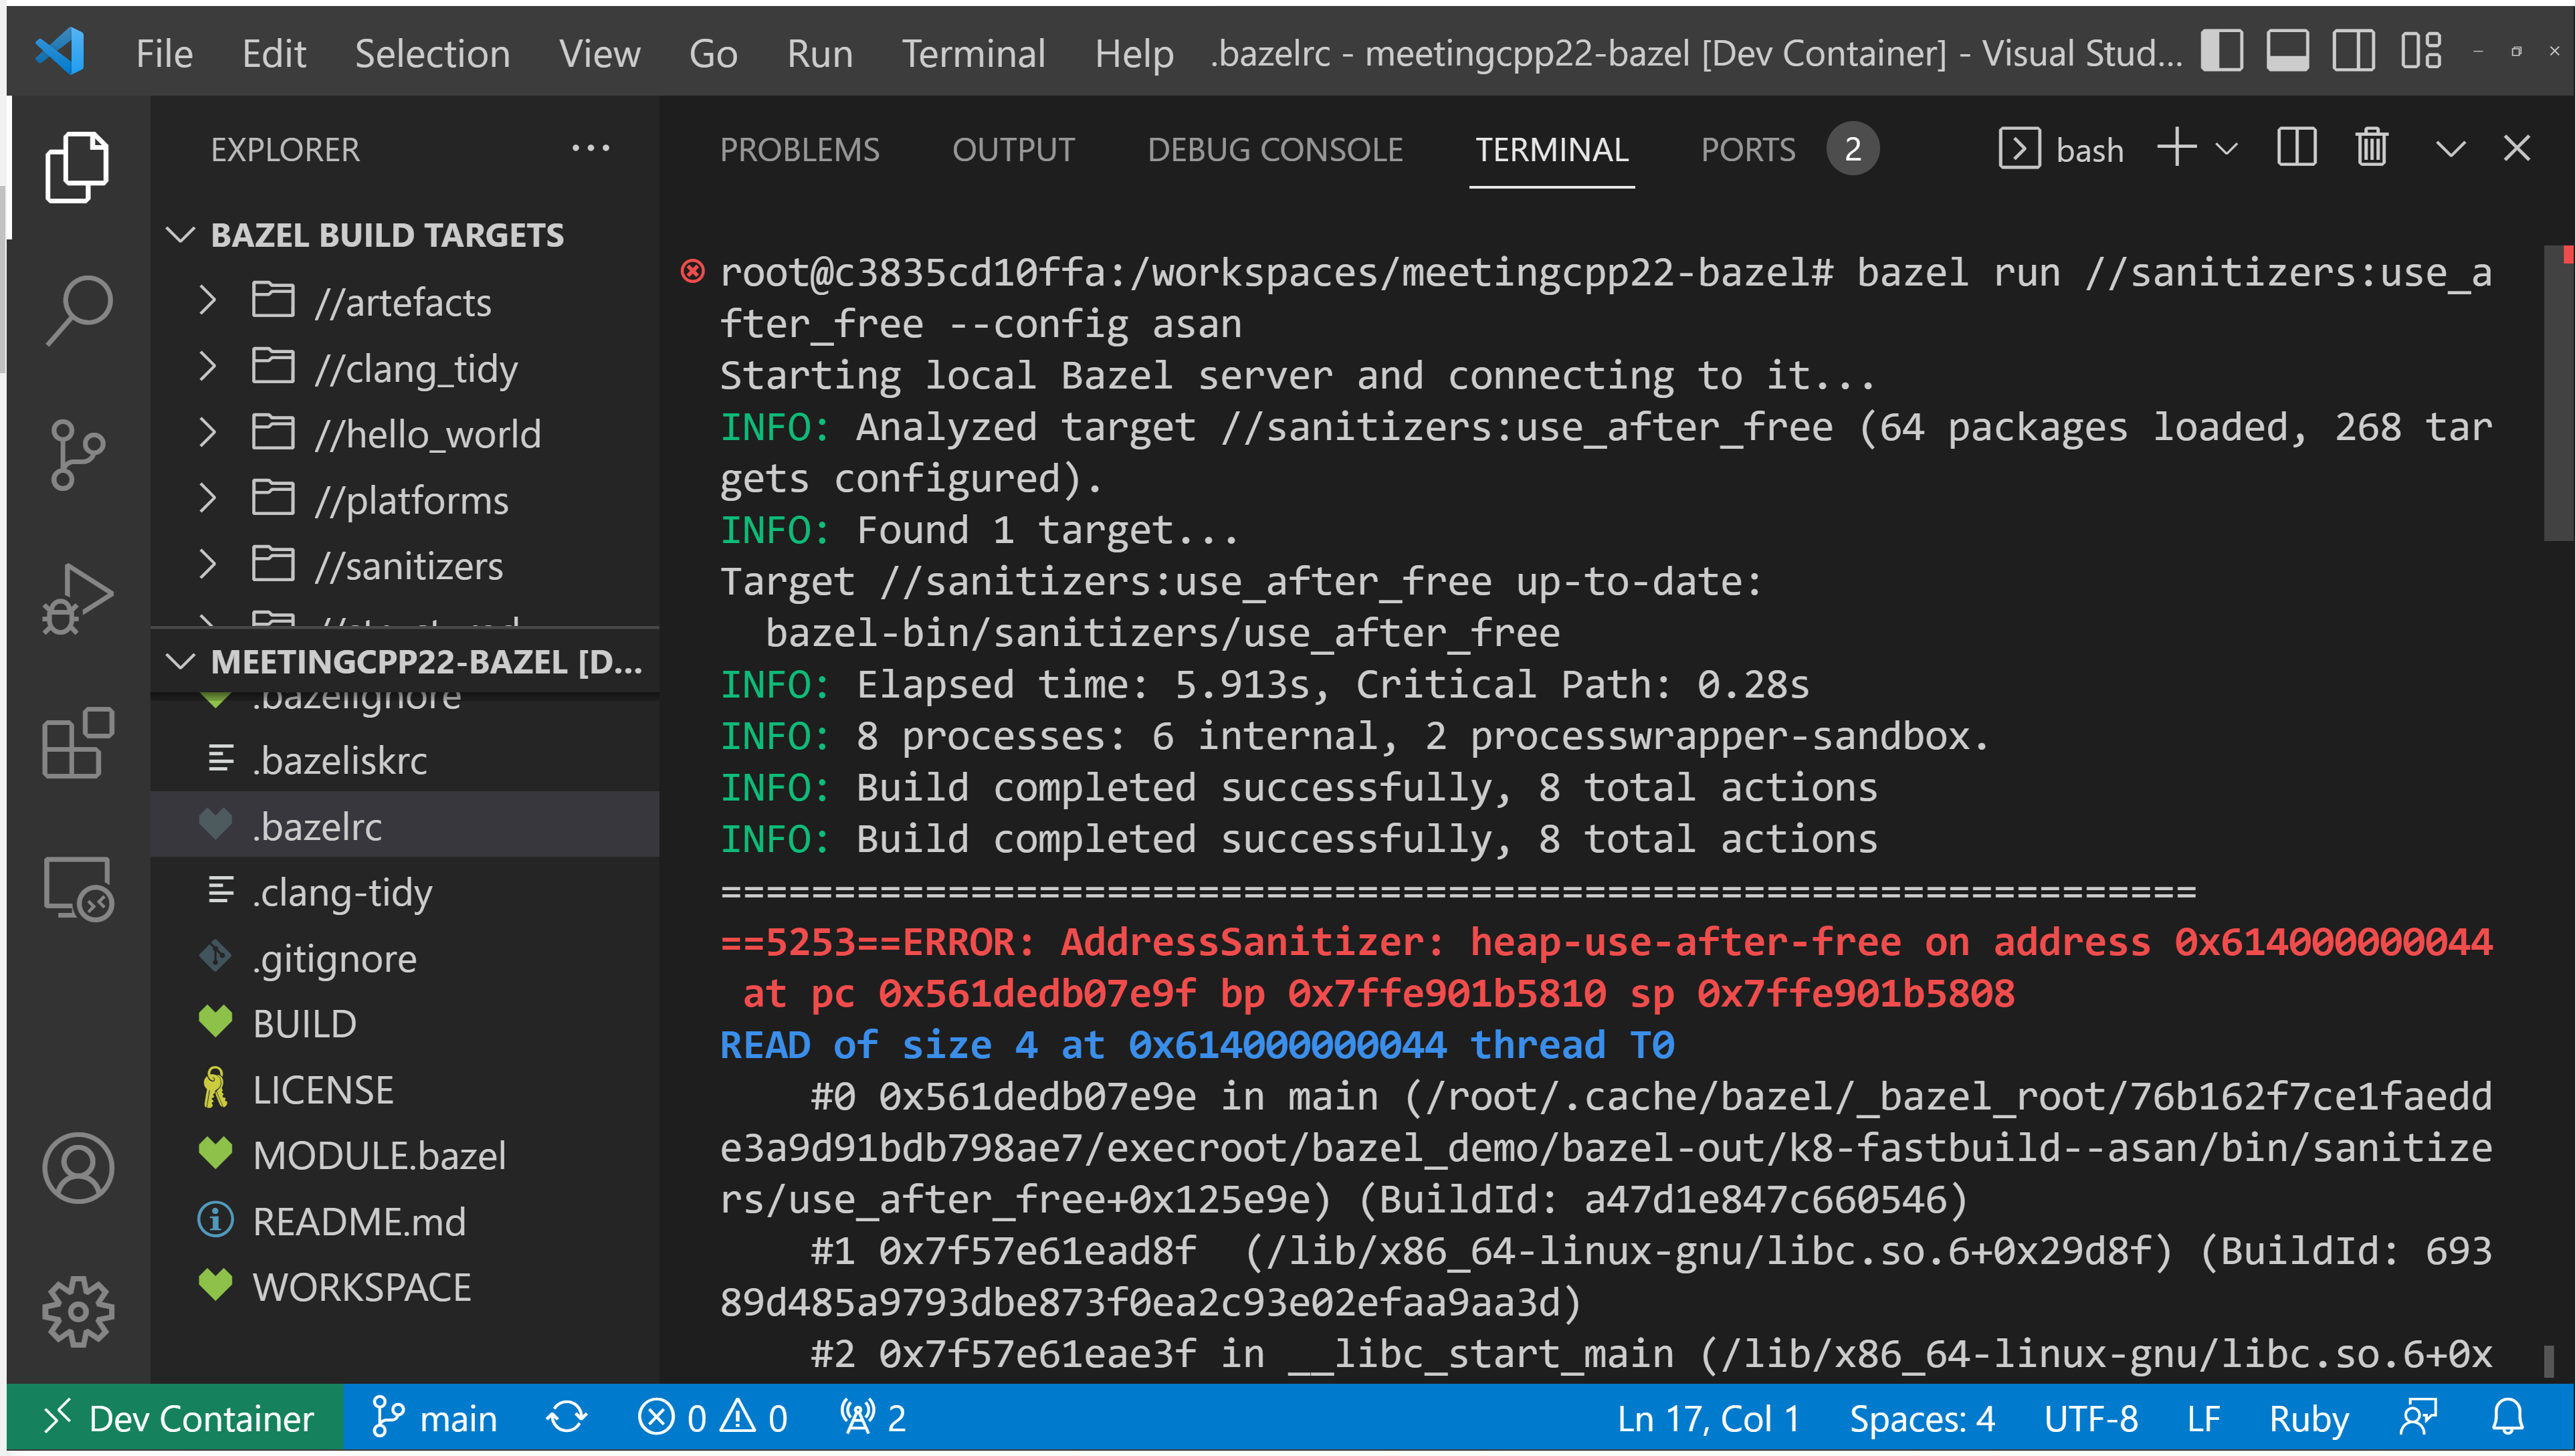
\includegraphics[width=\paperwidth]{slides/static_demos/03_01_run.png}}
\begin{frame}[plain]
\end{frame}
}

{
\usebackgroundtemplate{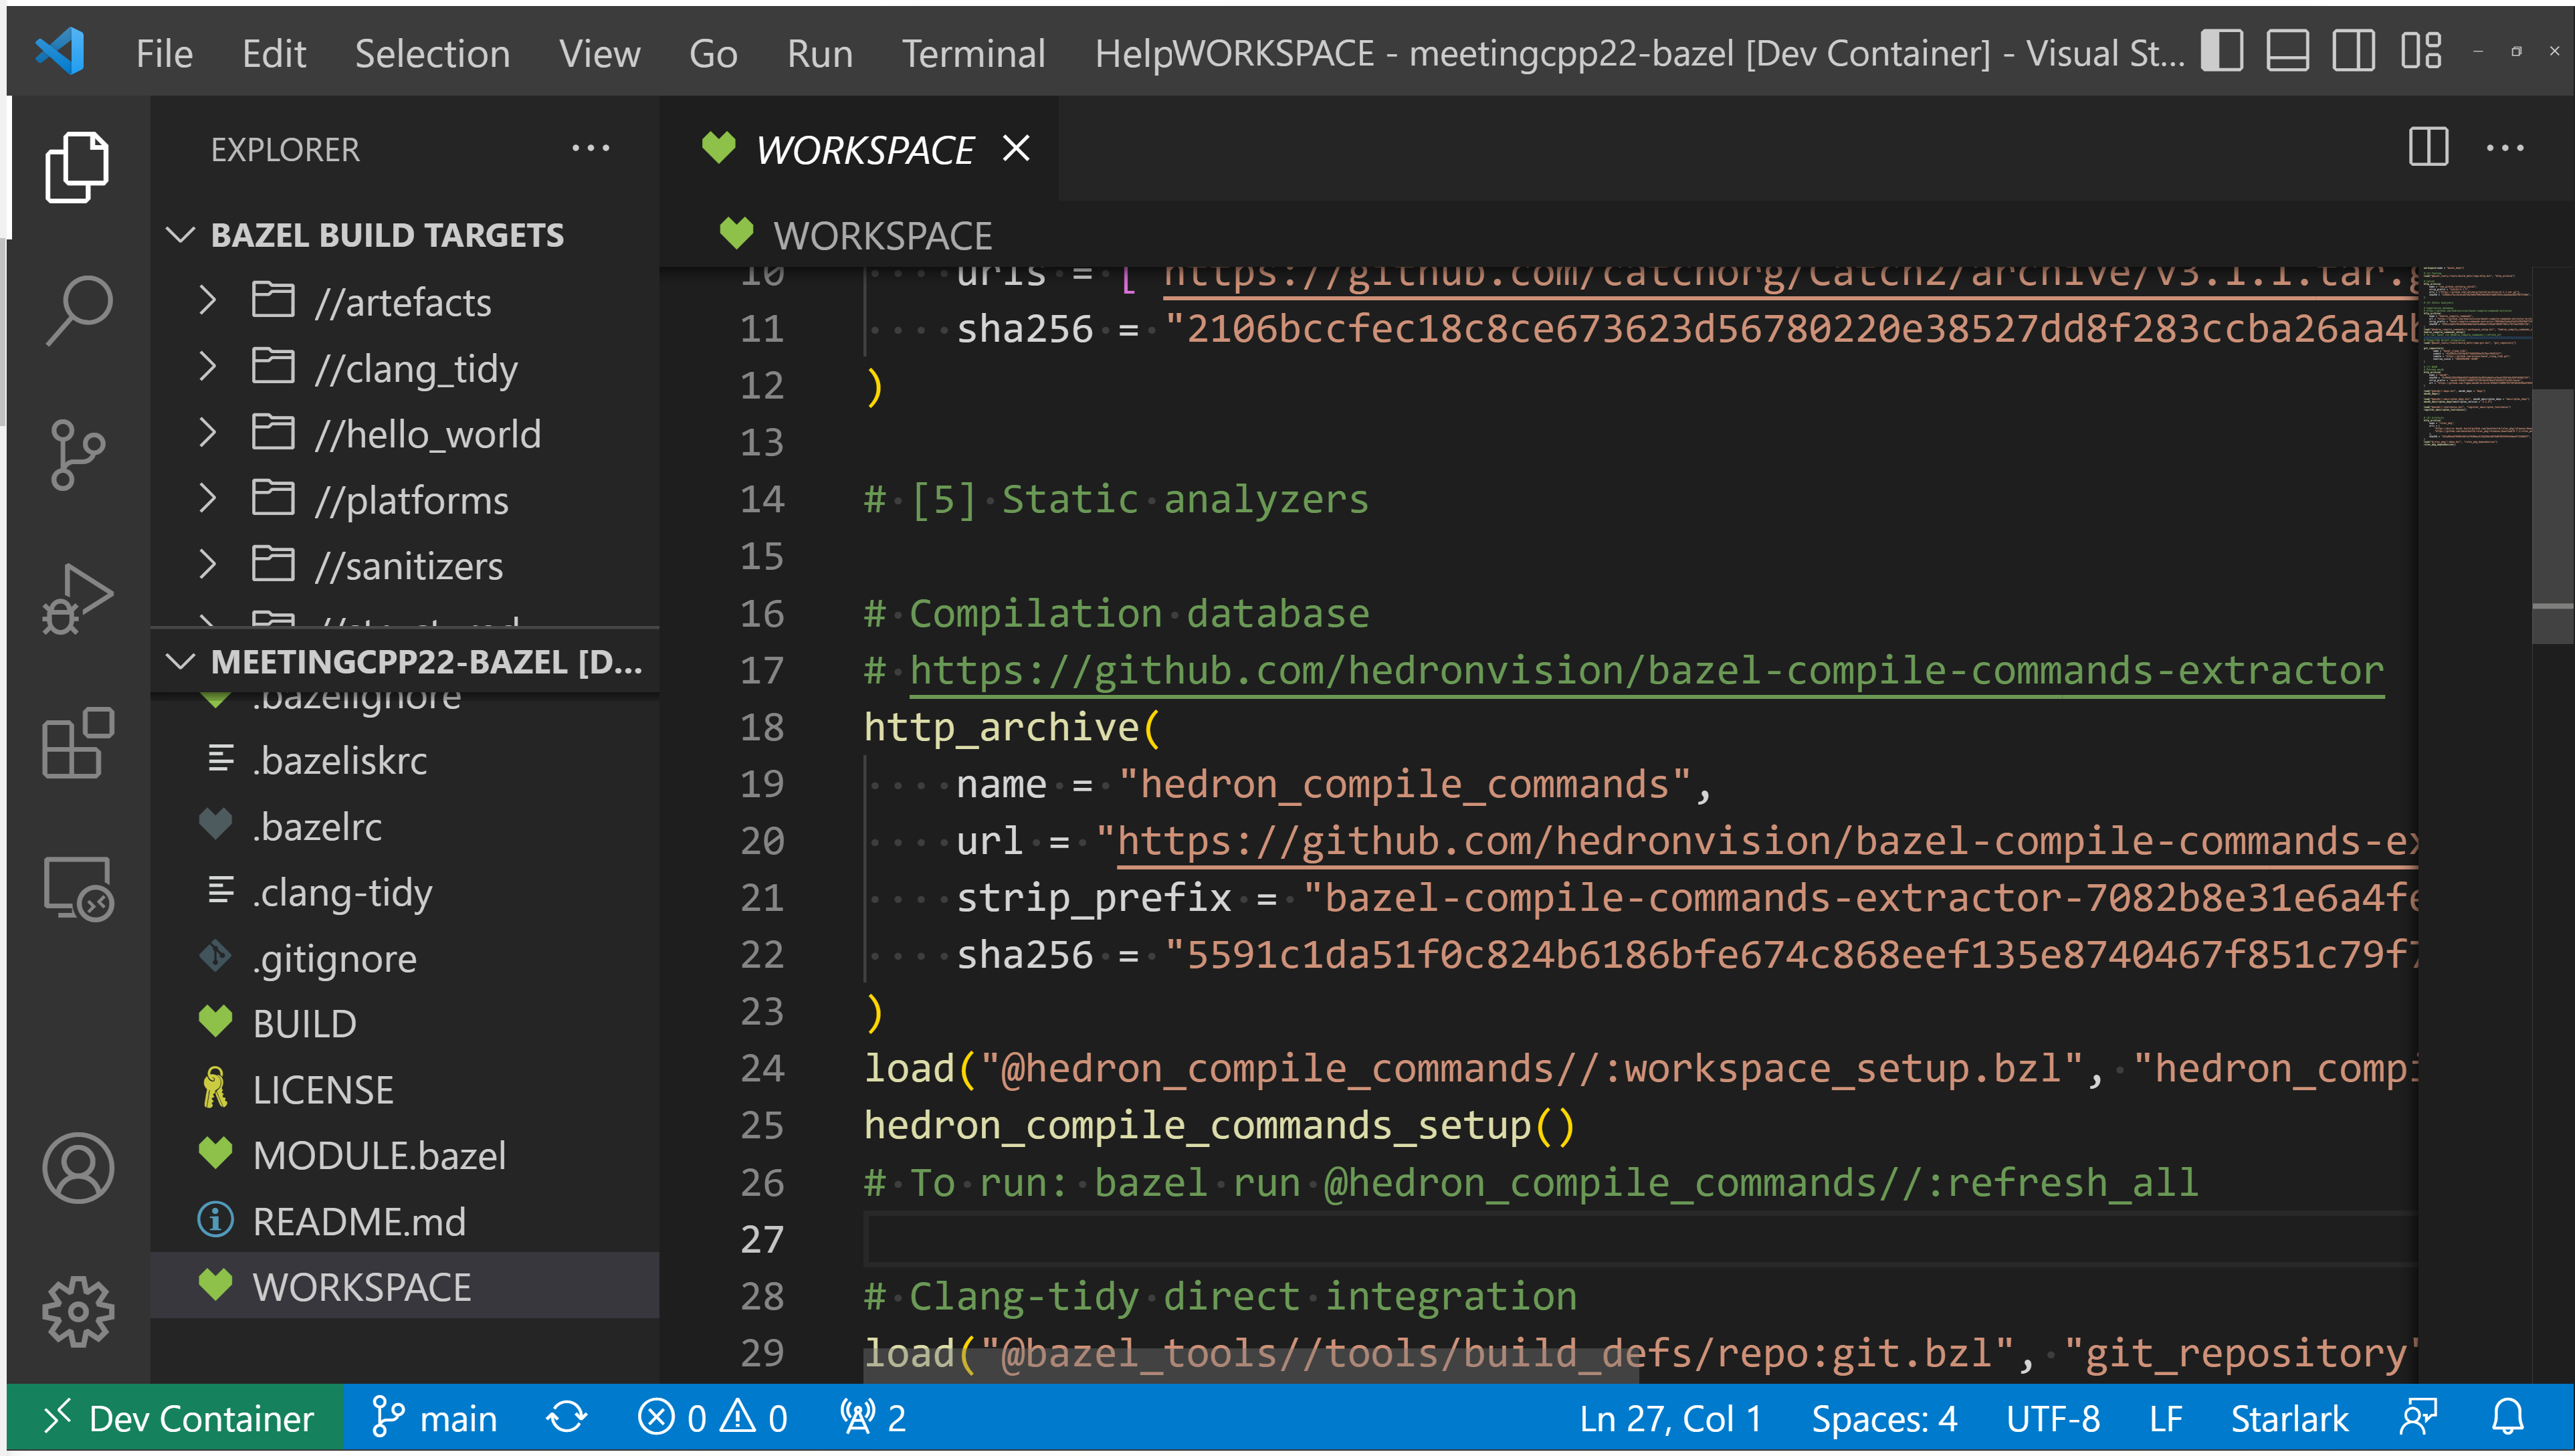
\includegraphics[width=\paperwidth]{slides/static_demos/03_02_compilation_db.png}}
\begin{frame}[plain]
\end{frame}
}

{
\usebackgroundtemplate{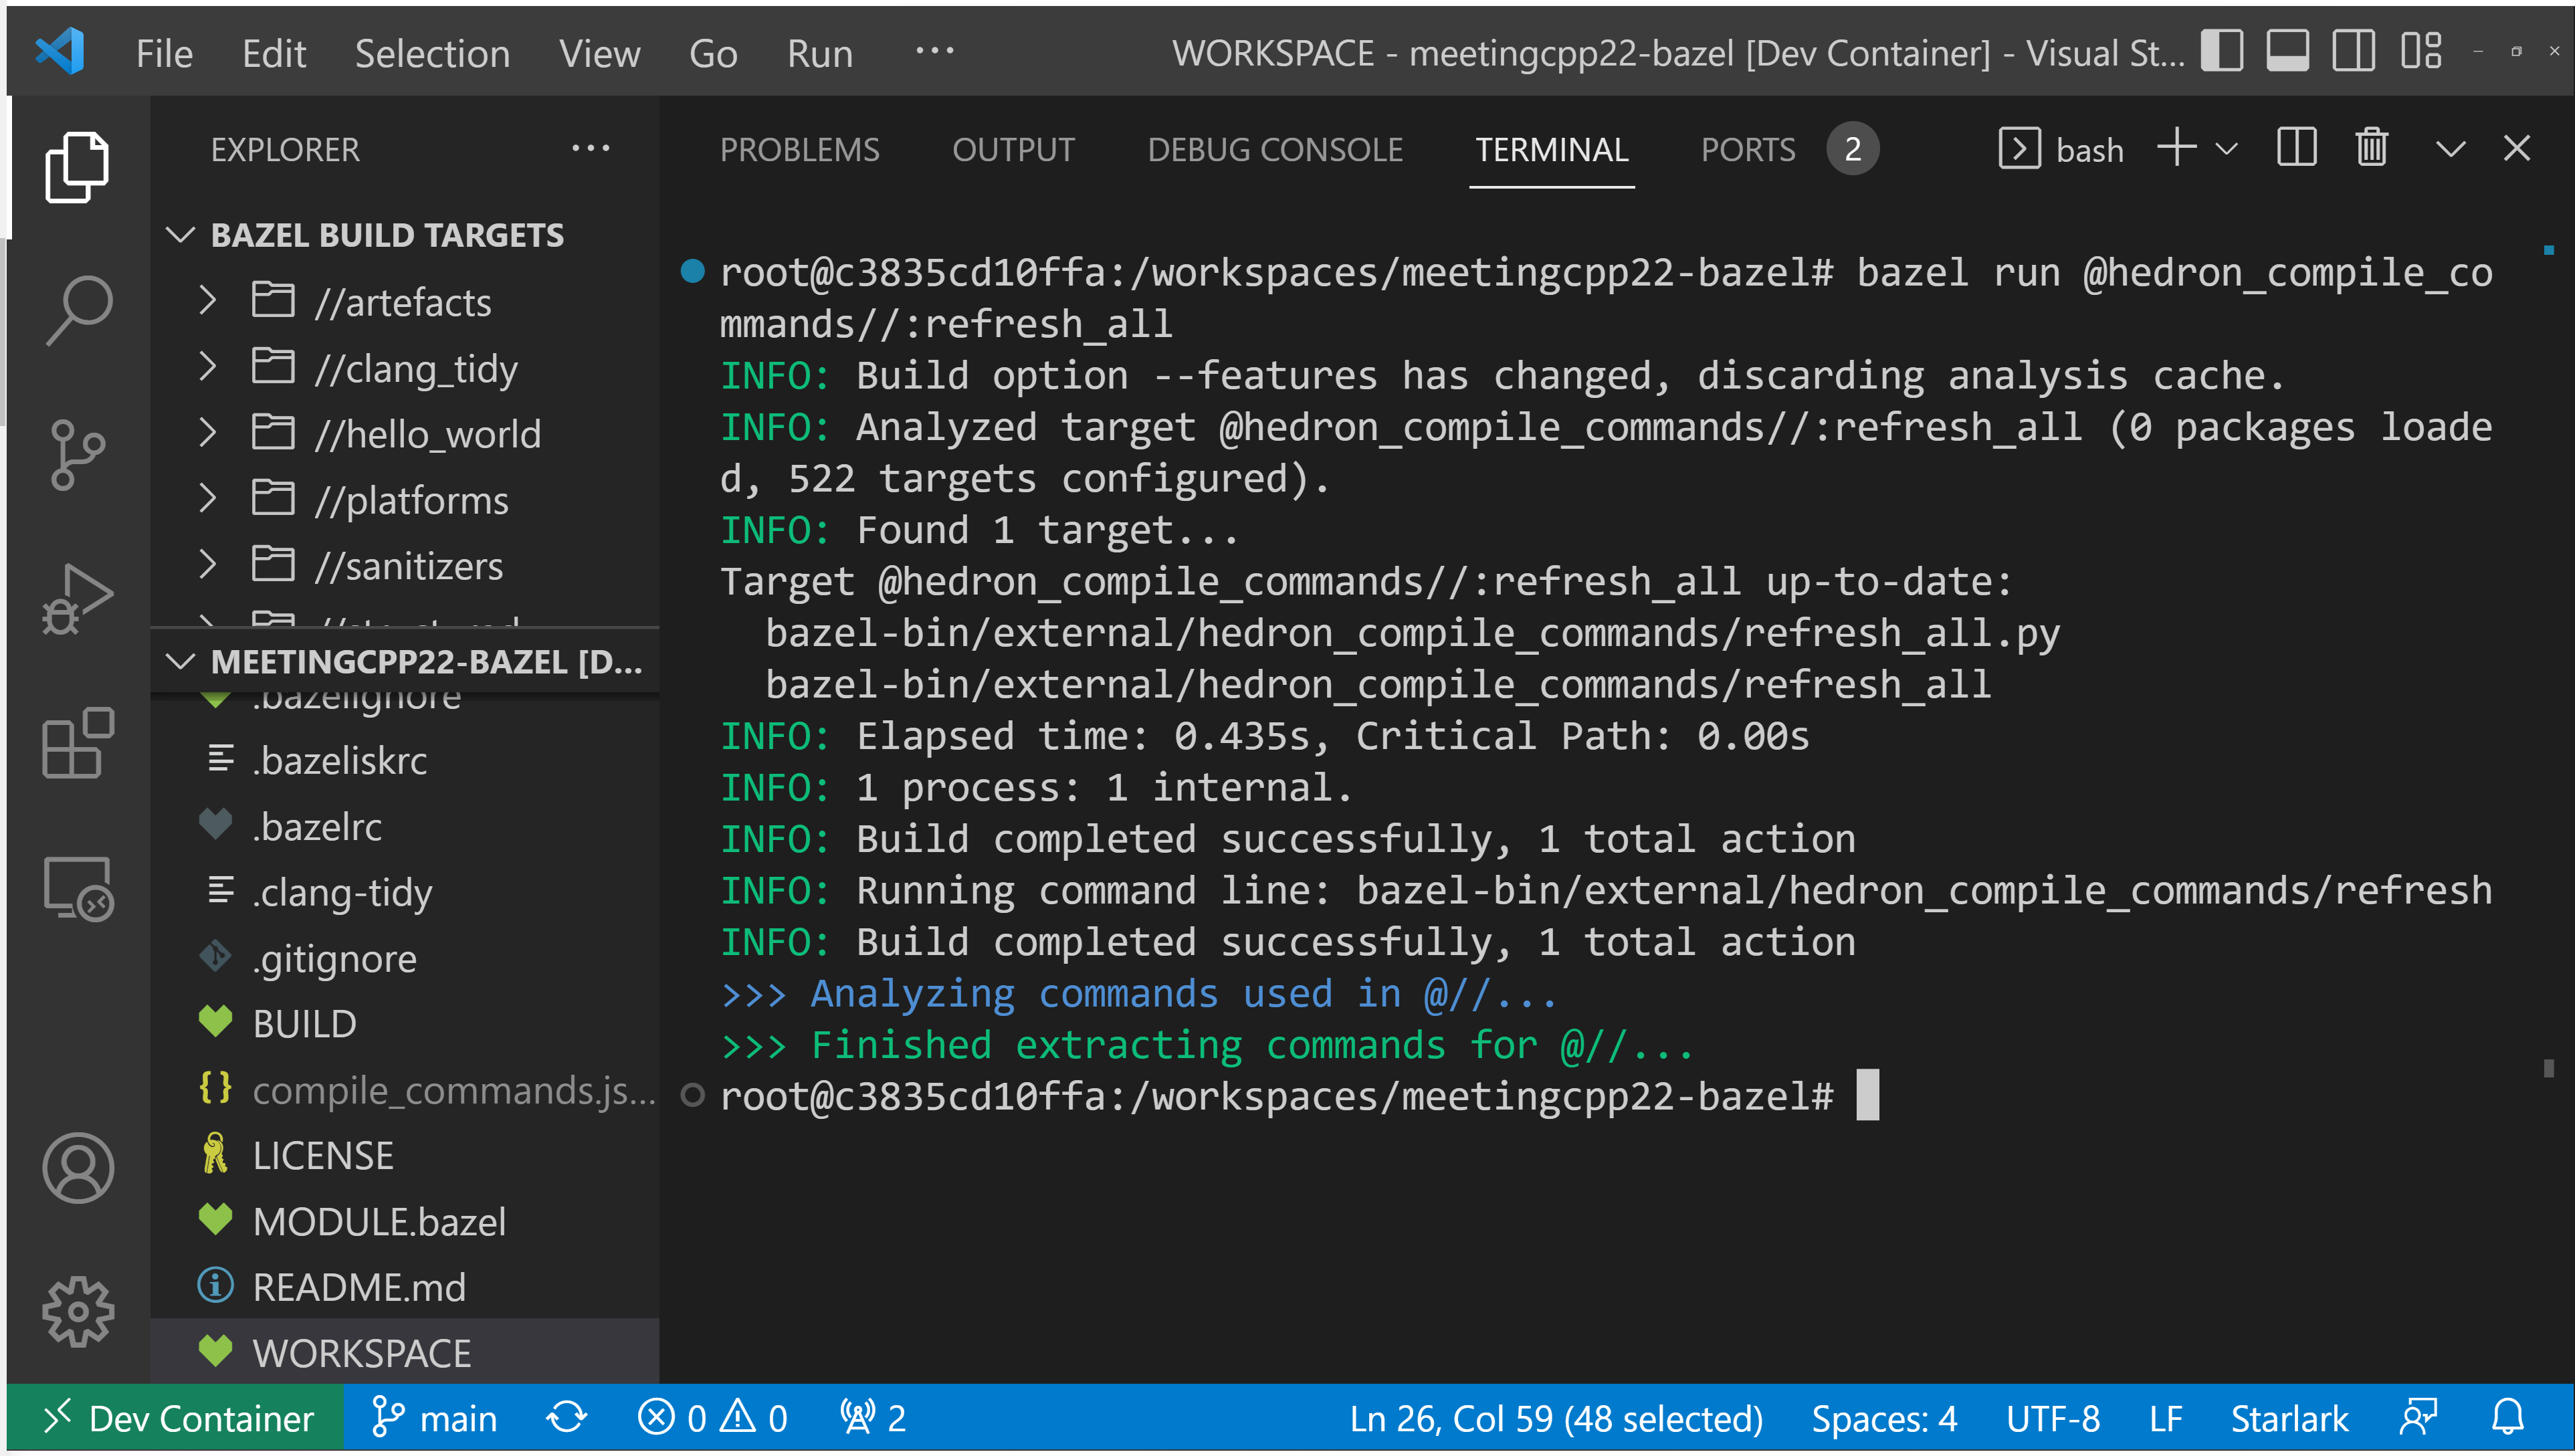
\includegraphics[width=\paperwidth]{slides/static_demos/03_03_compilation_db_run.png}}
\begin{frame}[plain]
\end{frame}
}

{
\usebackgroundtemplate{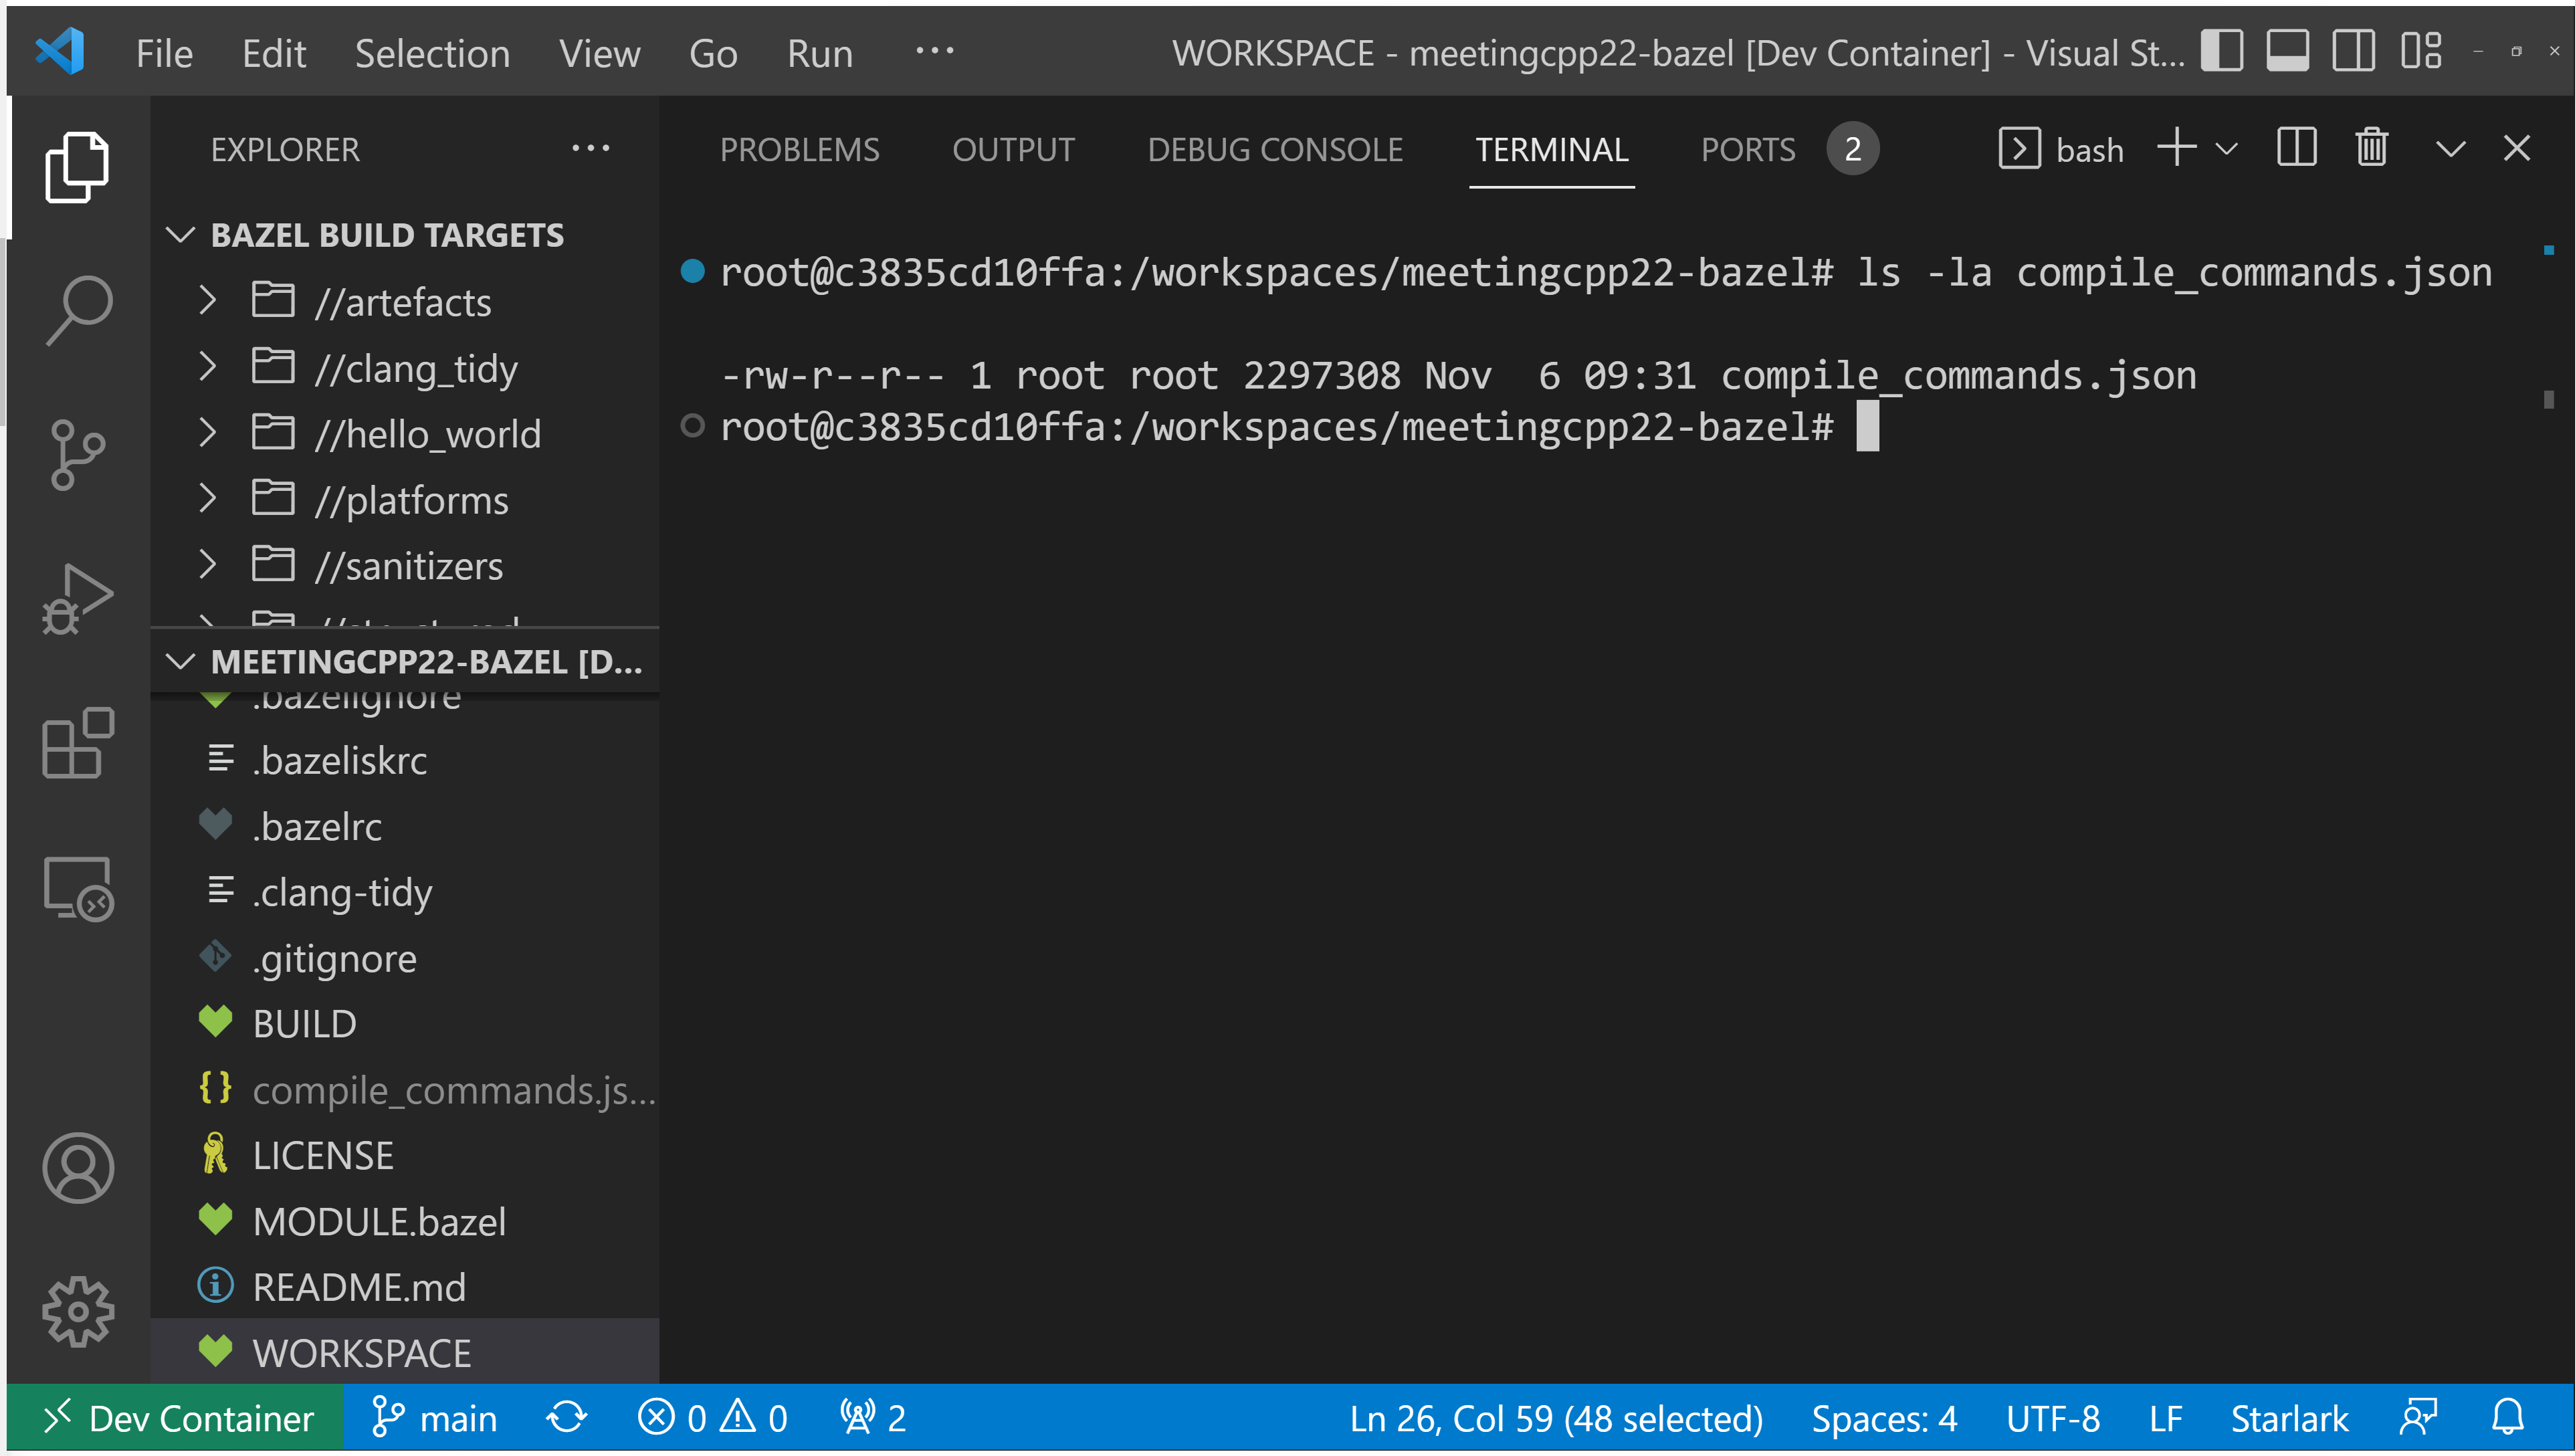
\includegraphics[width=\paperwidth]{slides/static_demos/03_04_compilation_db_file.png}}
\begin{frame}[plain]
\end{frame}
}

{
\usebackgroundtemplate{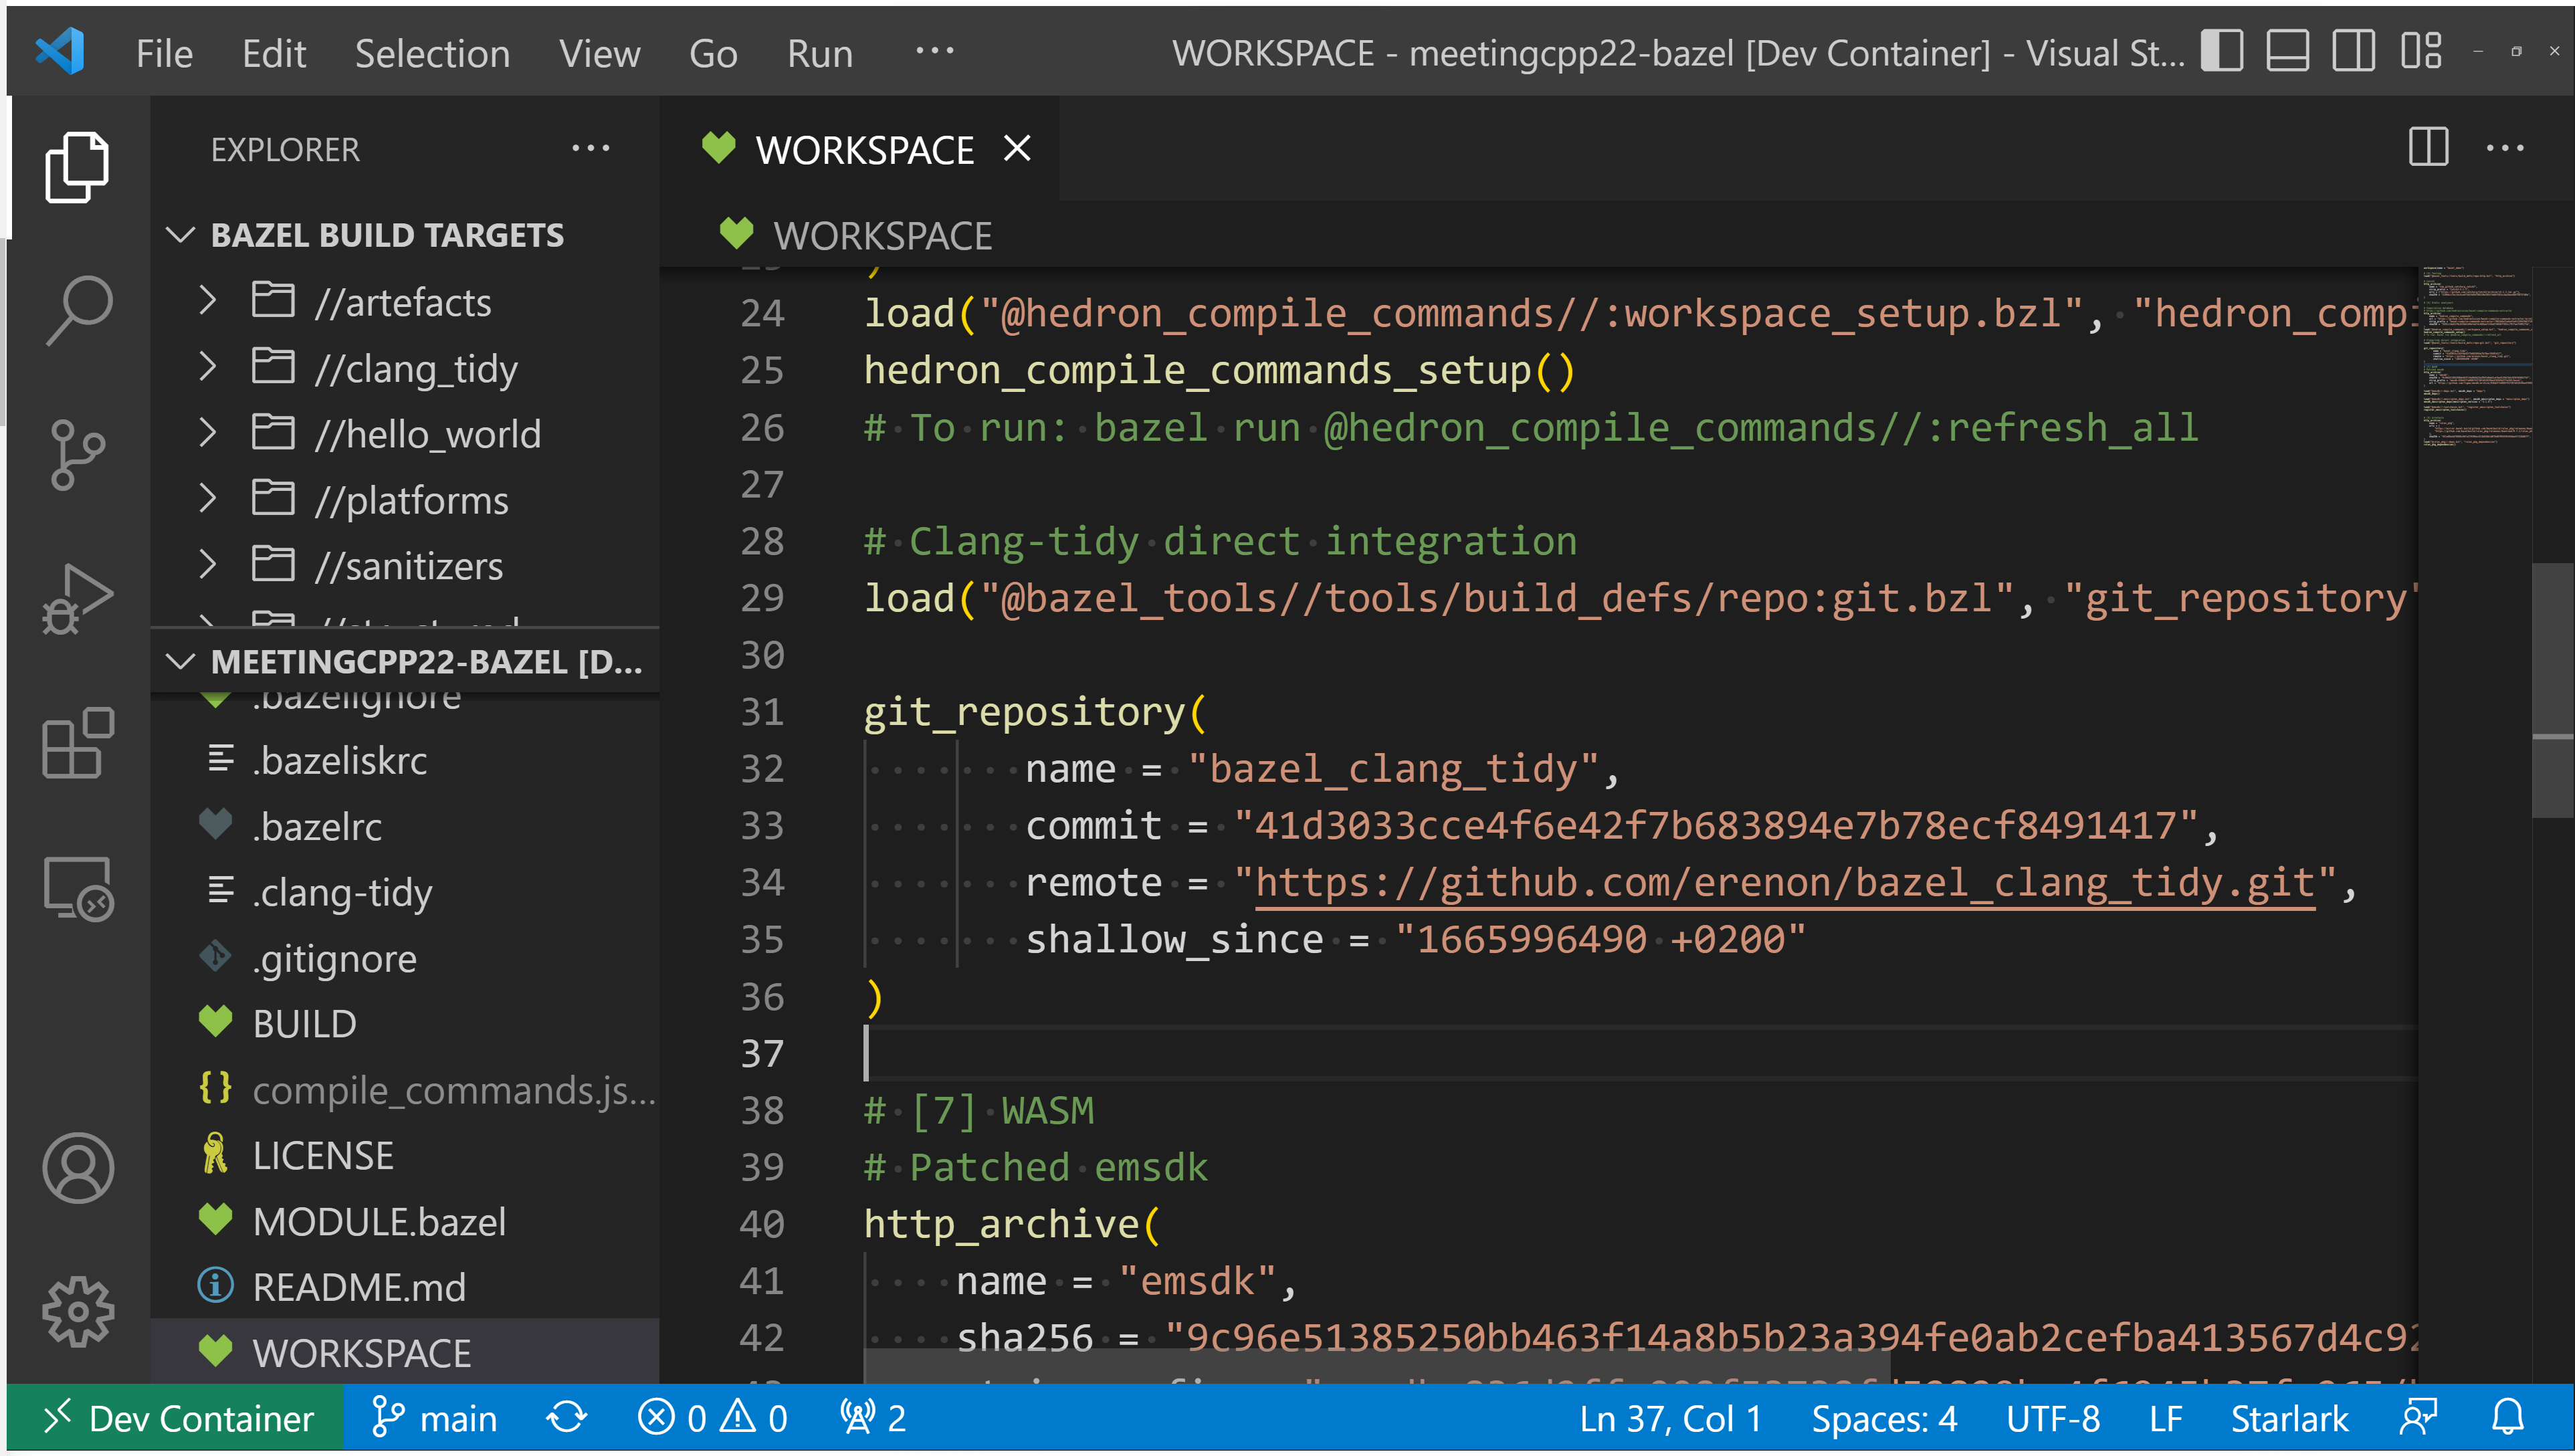
\includegraphics[width=\paperwidth]{slides/static_demos/04_00_workspace.png}}
\begin{frame}[plain]
\end{frame}
}

{
\usebackgroundtemplate{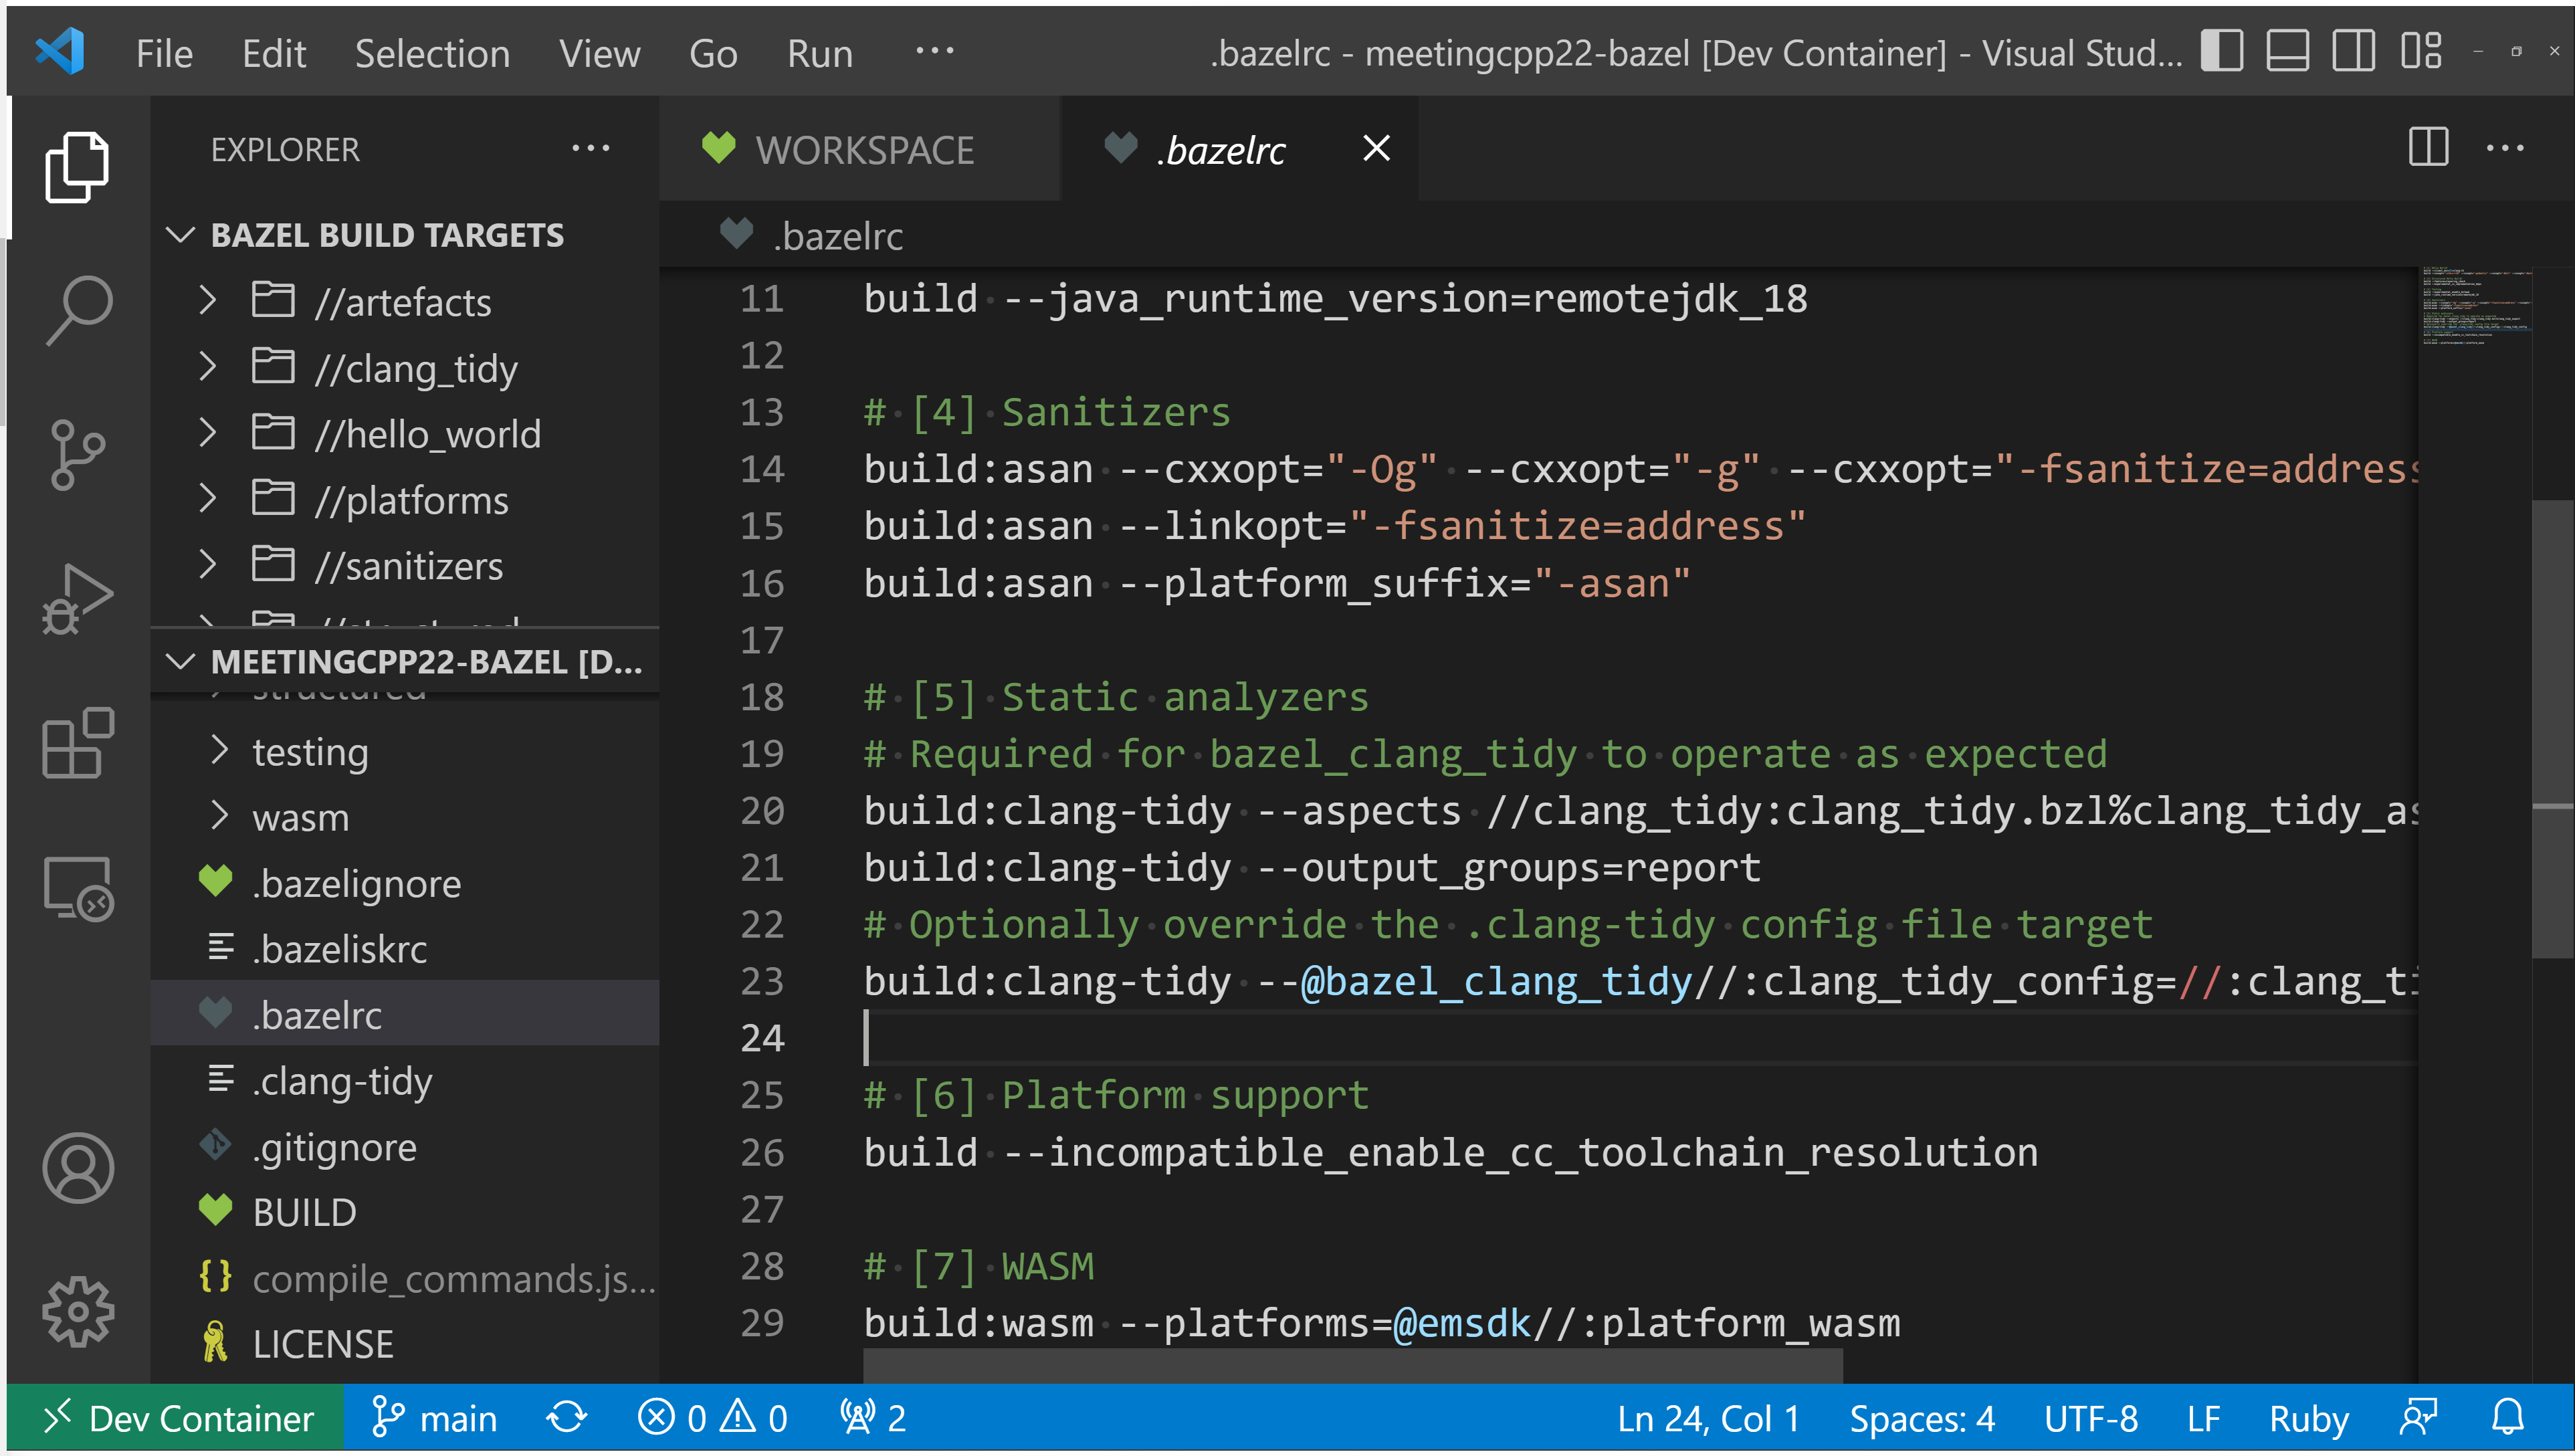
\includegraphics[width=\paperwidth]{slides/static_demos/04_01_bazelrc.png}}
\begin{frame}[plain]
\end{frame}
}

{
\usebackgroundtemplate{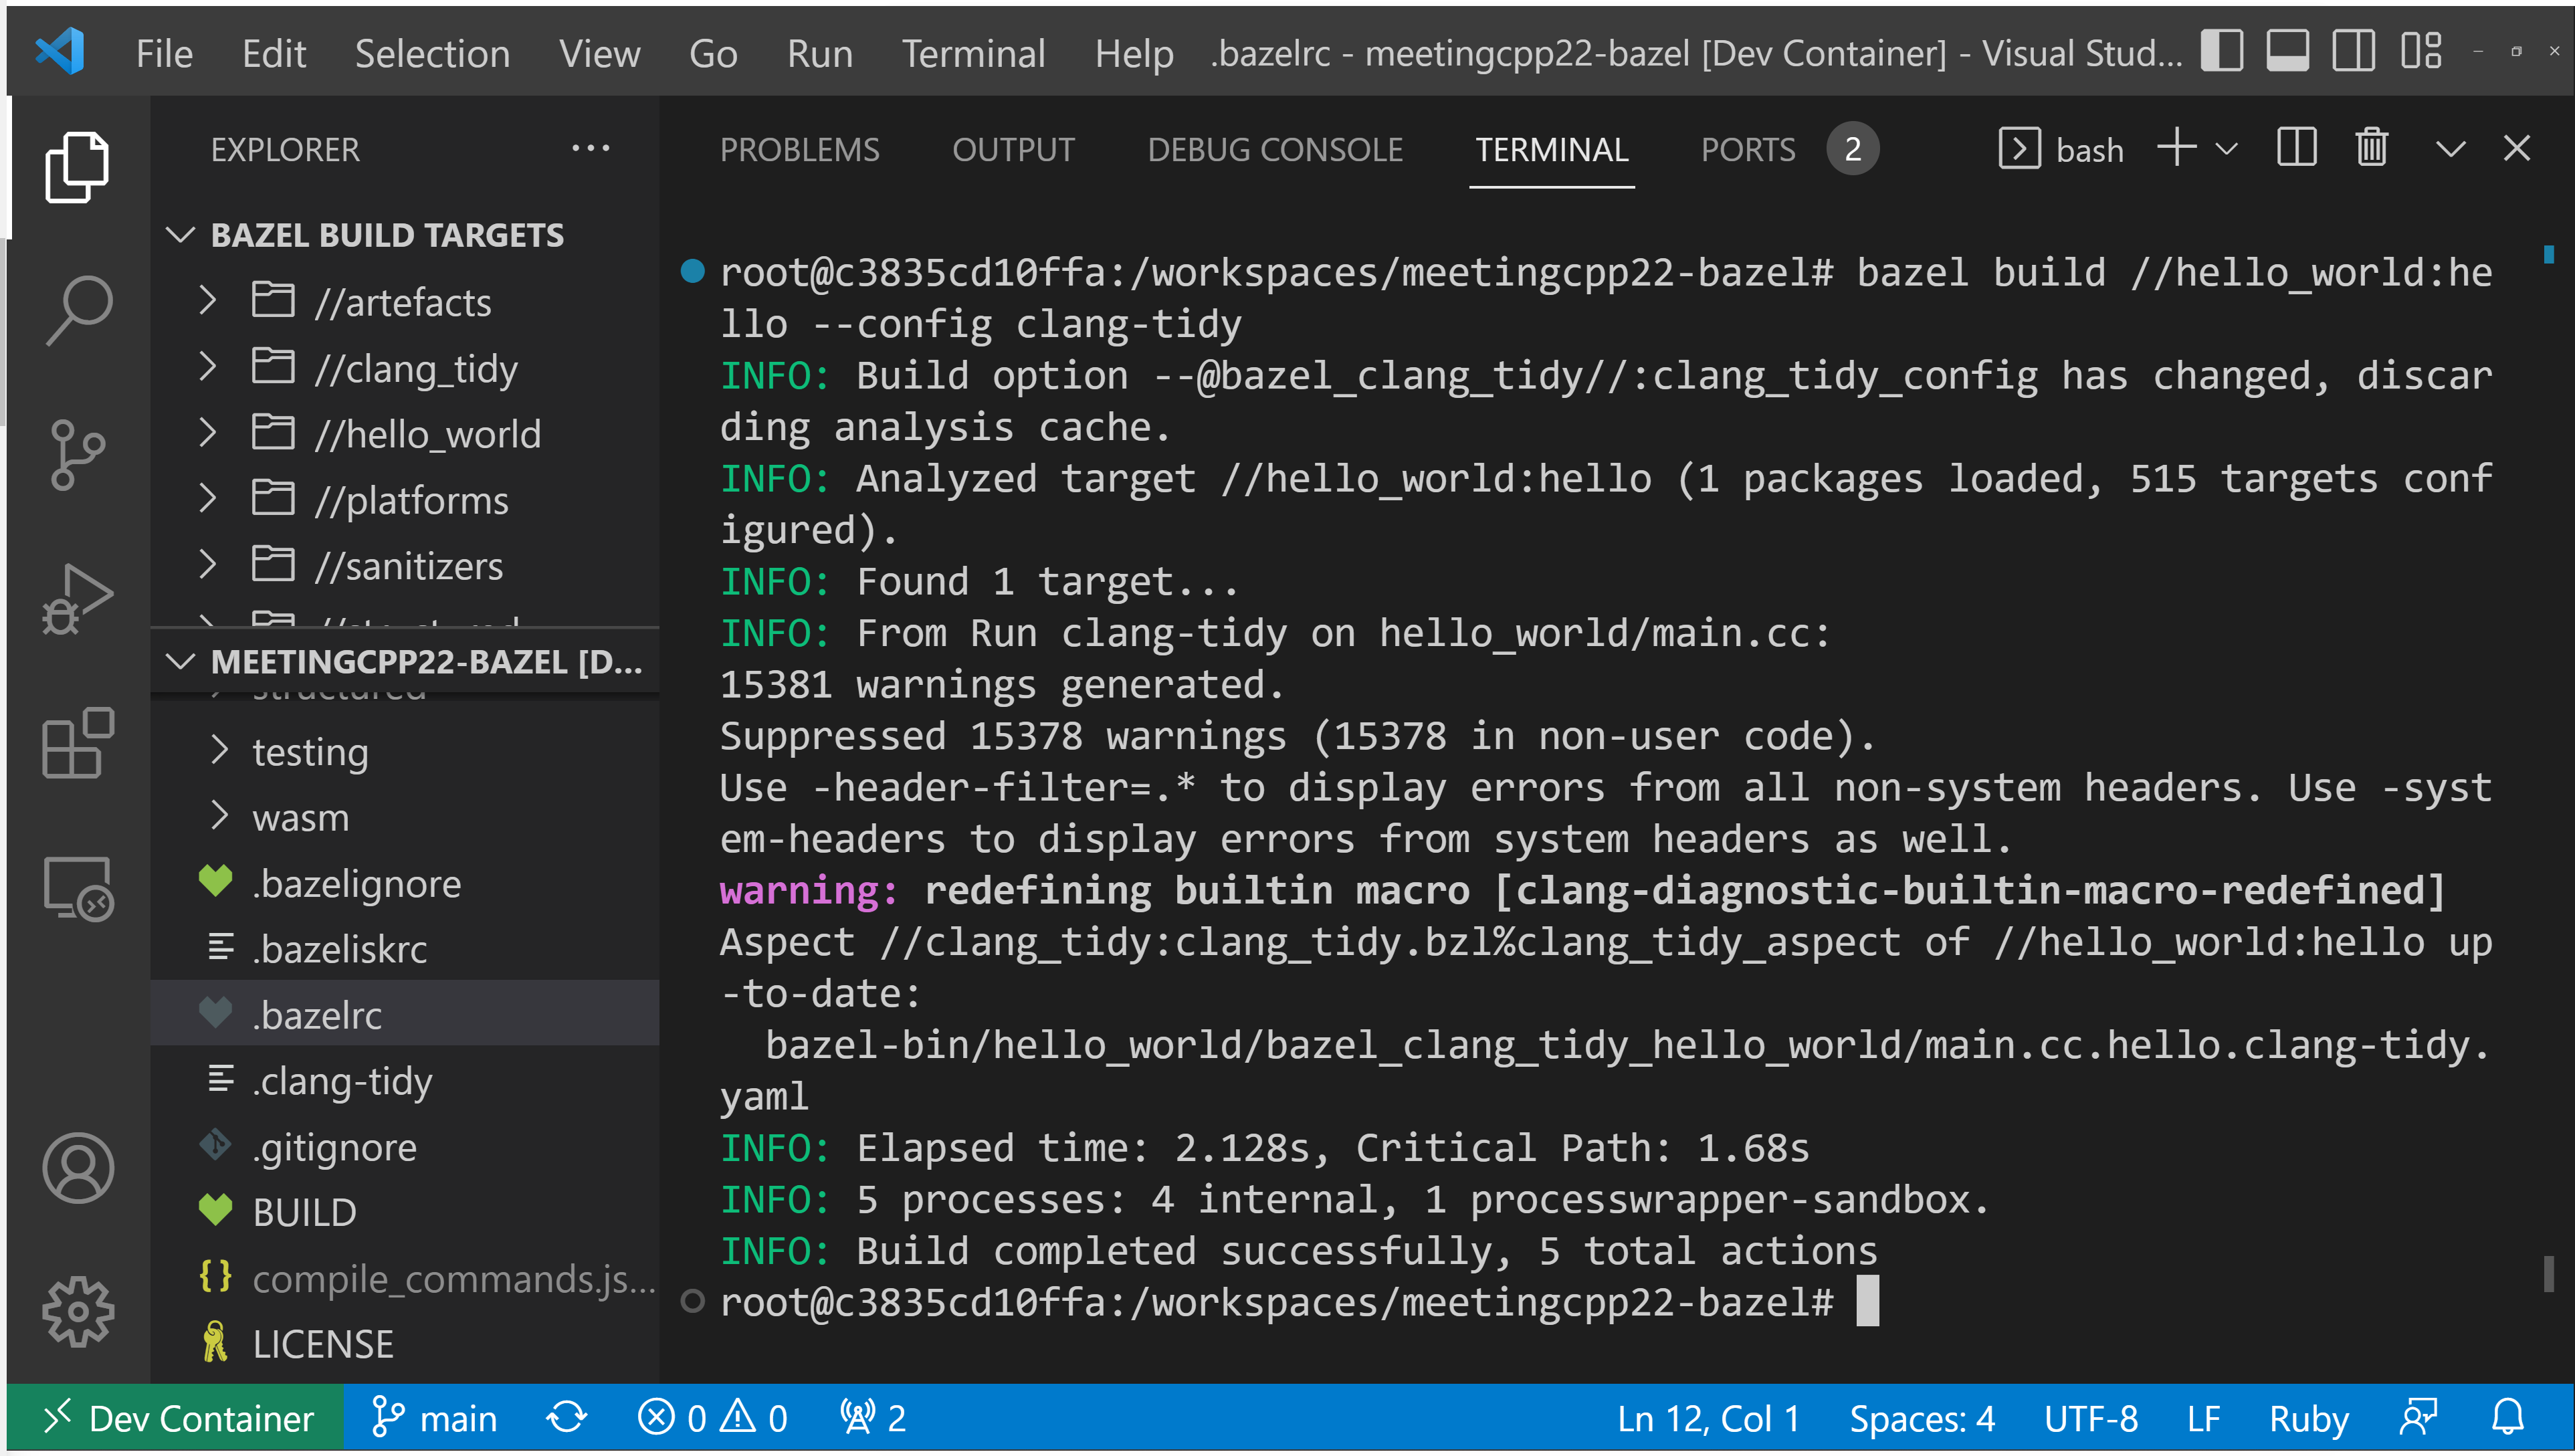
\includegraphics[width=\paperwidth]{slides/static_demos/04_02_clean.png}}
\begin{frame}[plain]
\end{frame}
}

{
\usebackgroundtemplate{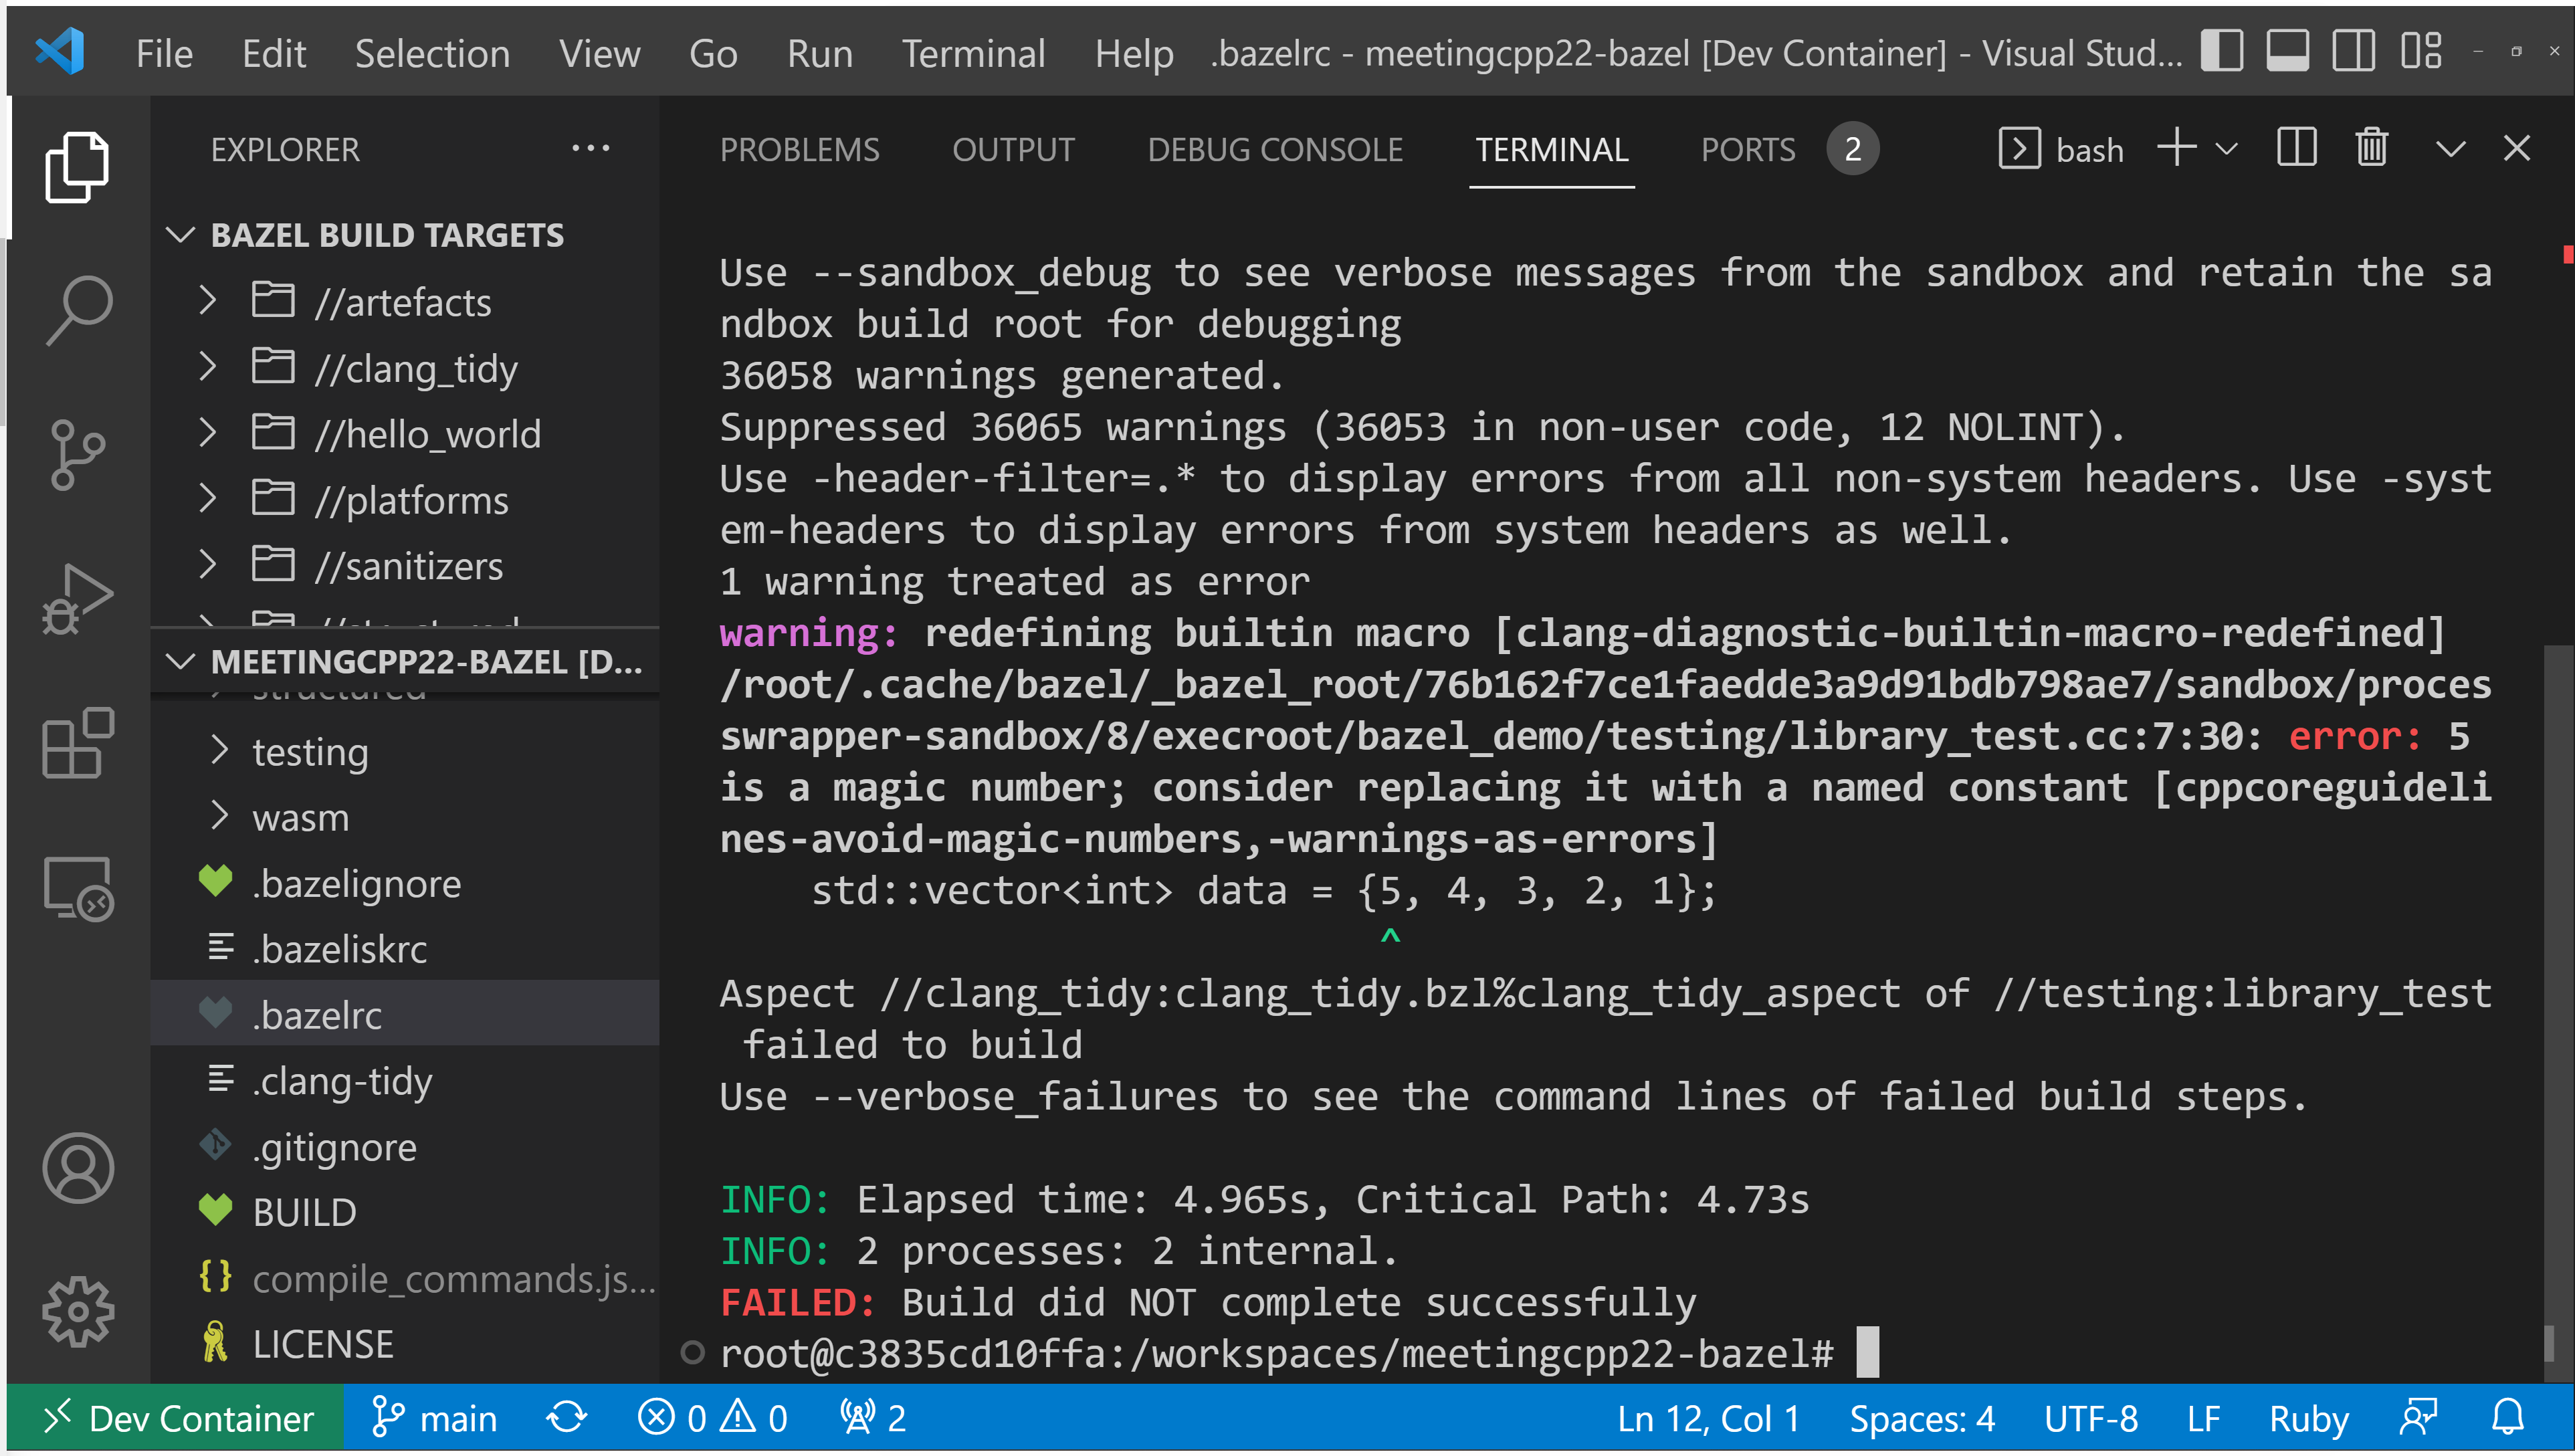
\includegraphics[width=\paperwidth]{slides/static_demos/04_03_unclean.png}}
\begin{frame}[plain]
\end{frame}
}

\begin{frame}{}
    \begin{center}
        \begin{Huge}Platforms\end{Huge}
    \end{center}
\end{frame}

{
\usebackgroundtemplate{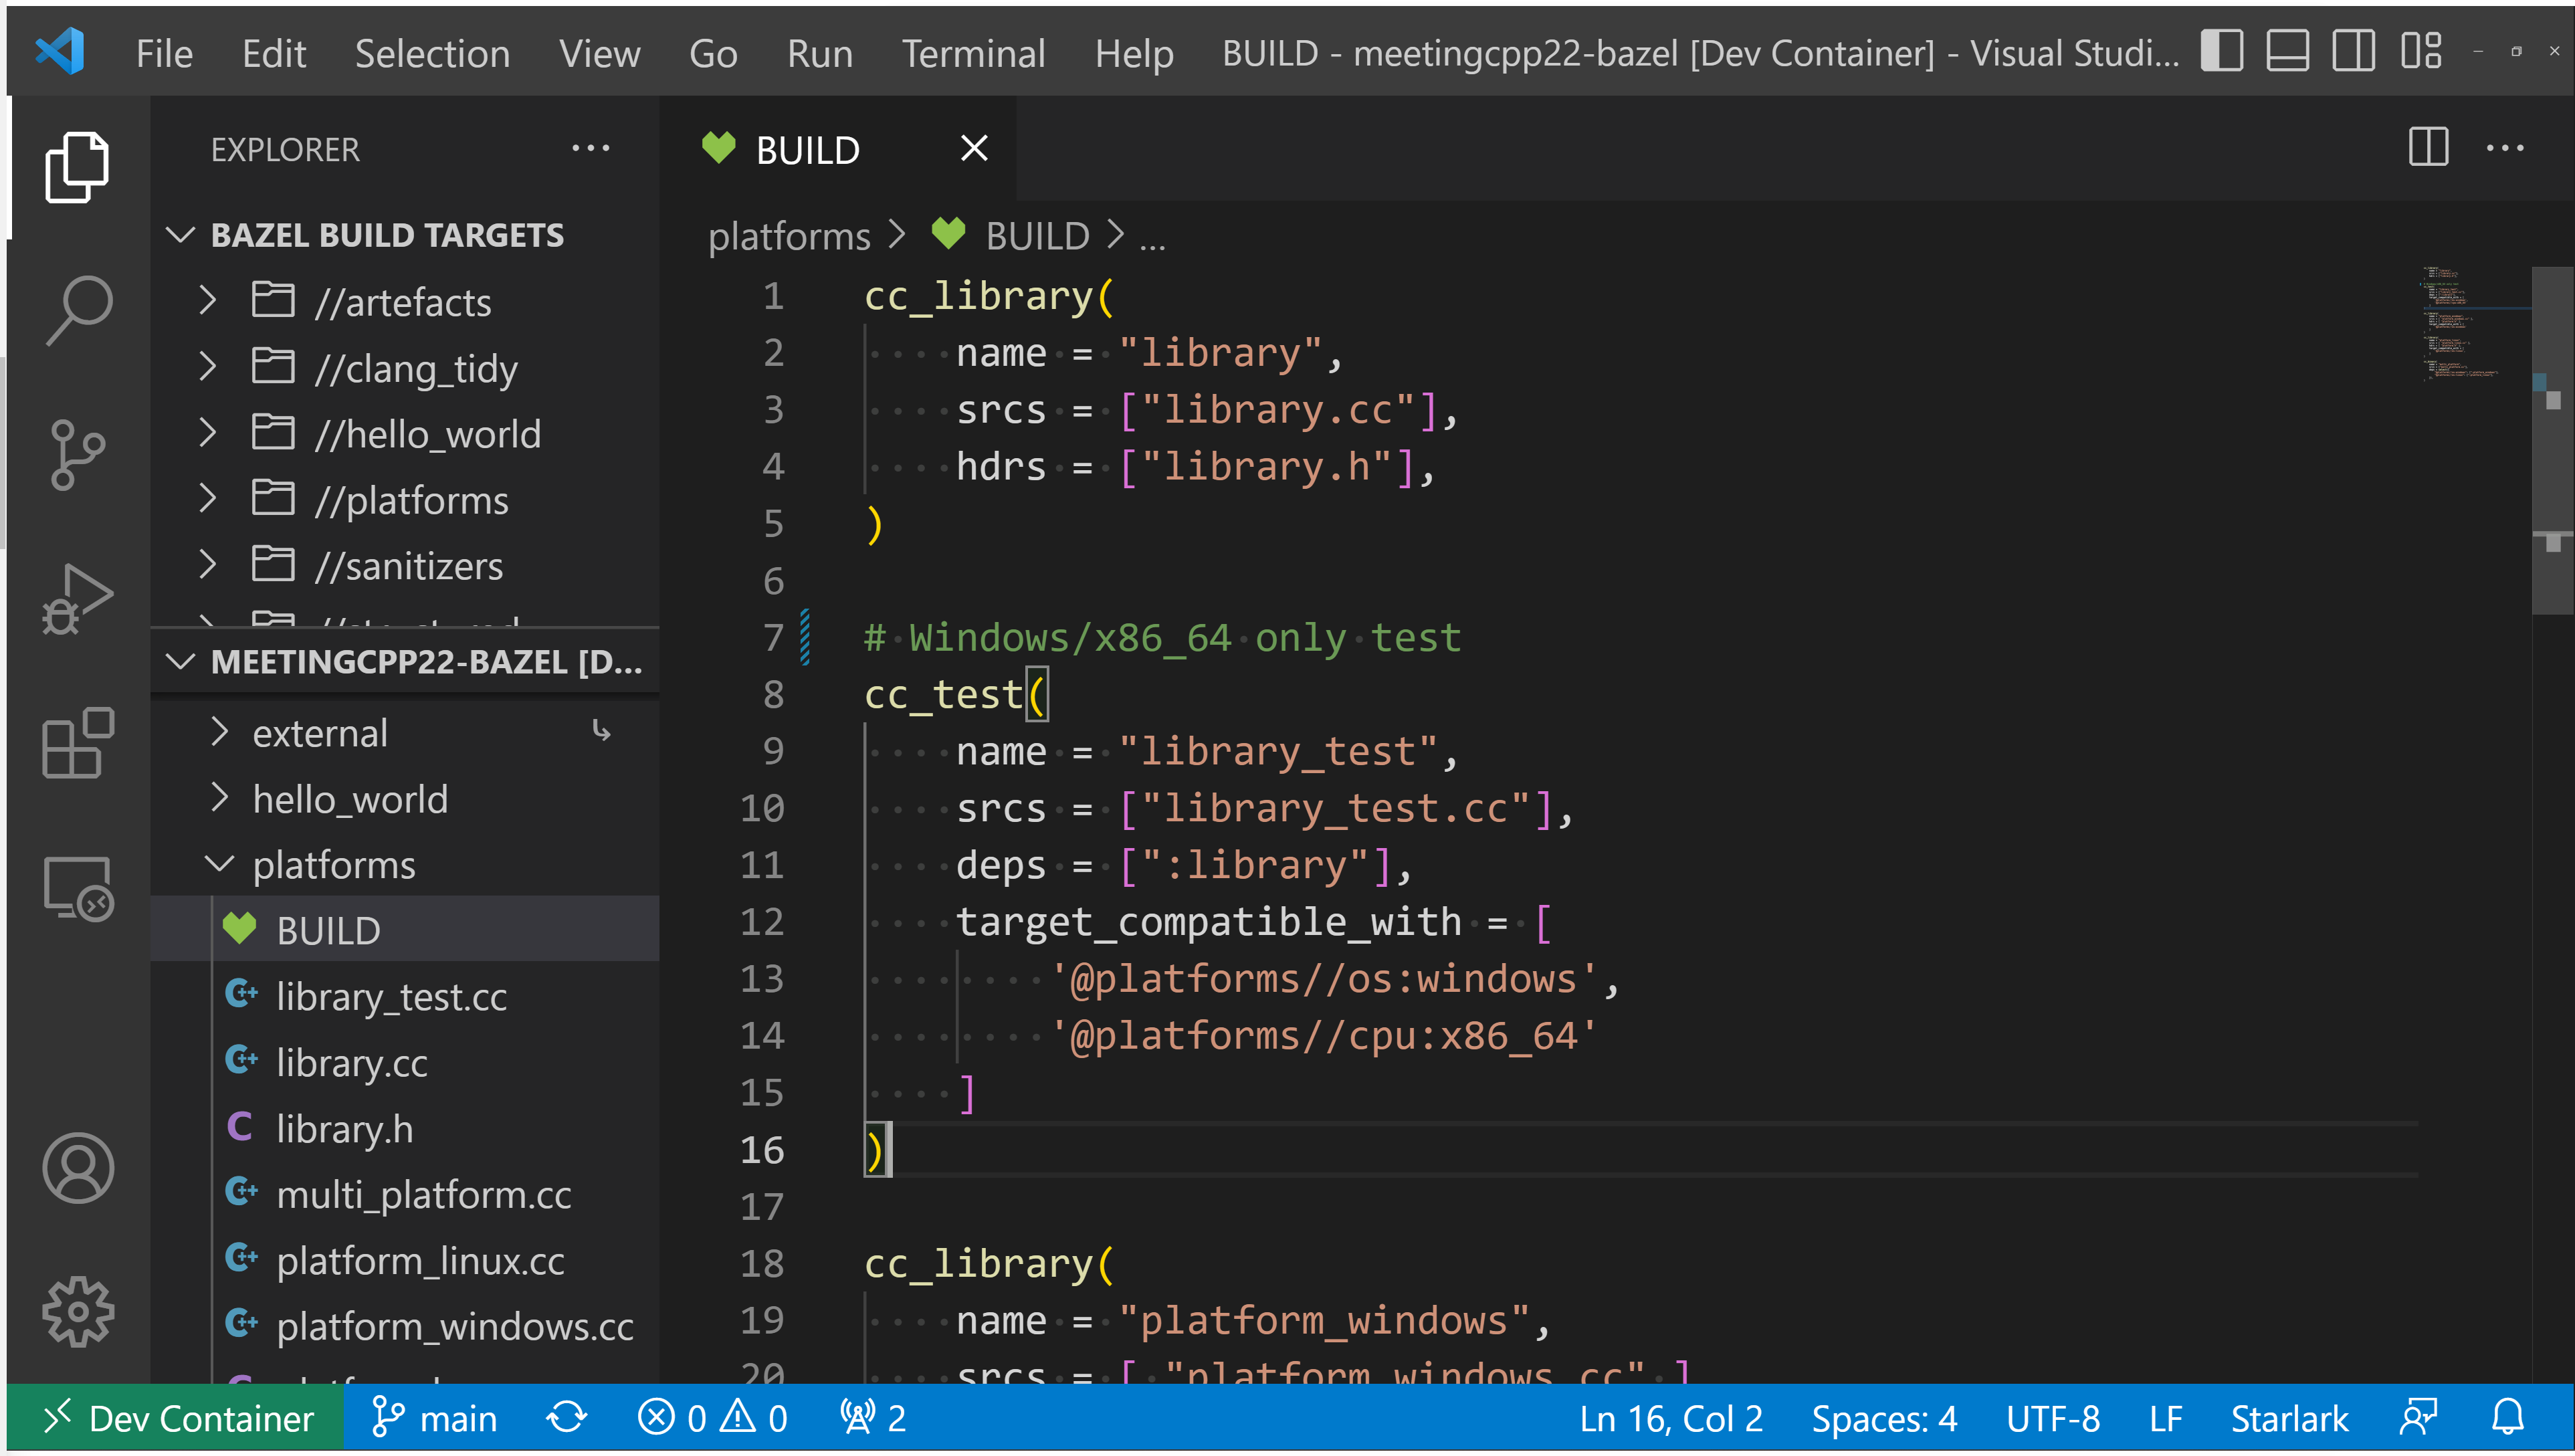
\includegraphics[width=\paperwidth]{slides/static_demos/05_00_platform_test.png}}
\begin{frame}[plain]
\end{frame}
}

{
\usebackgroundtemplate{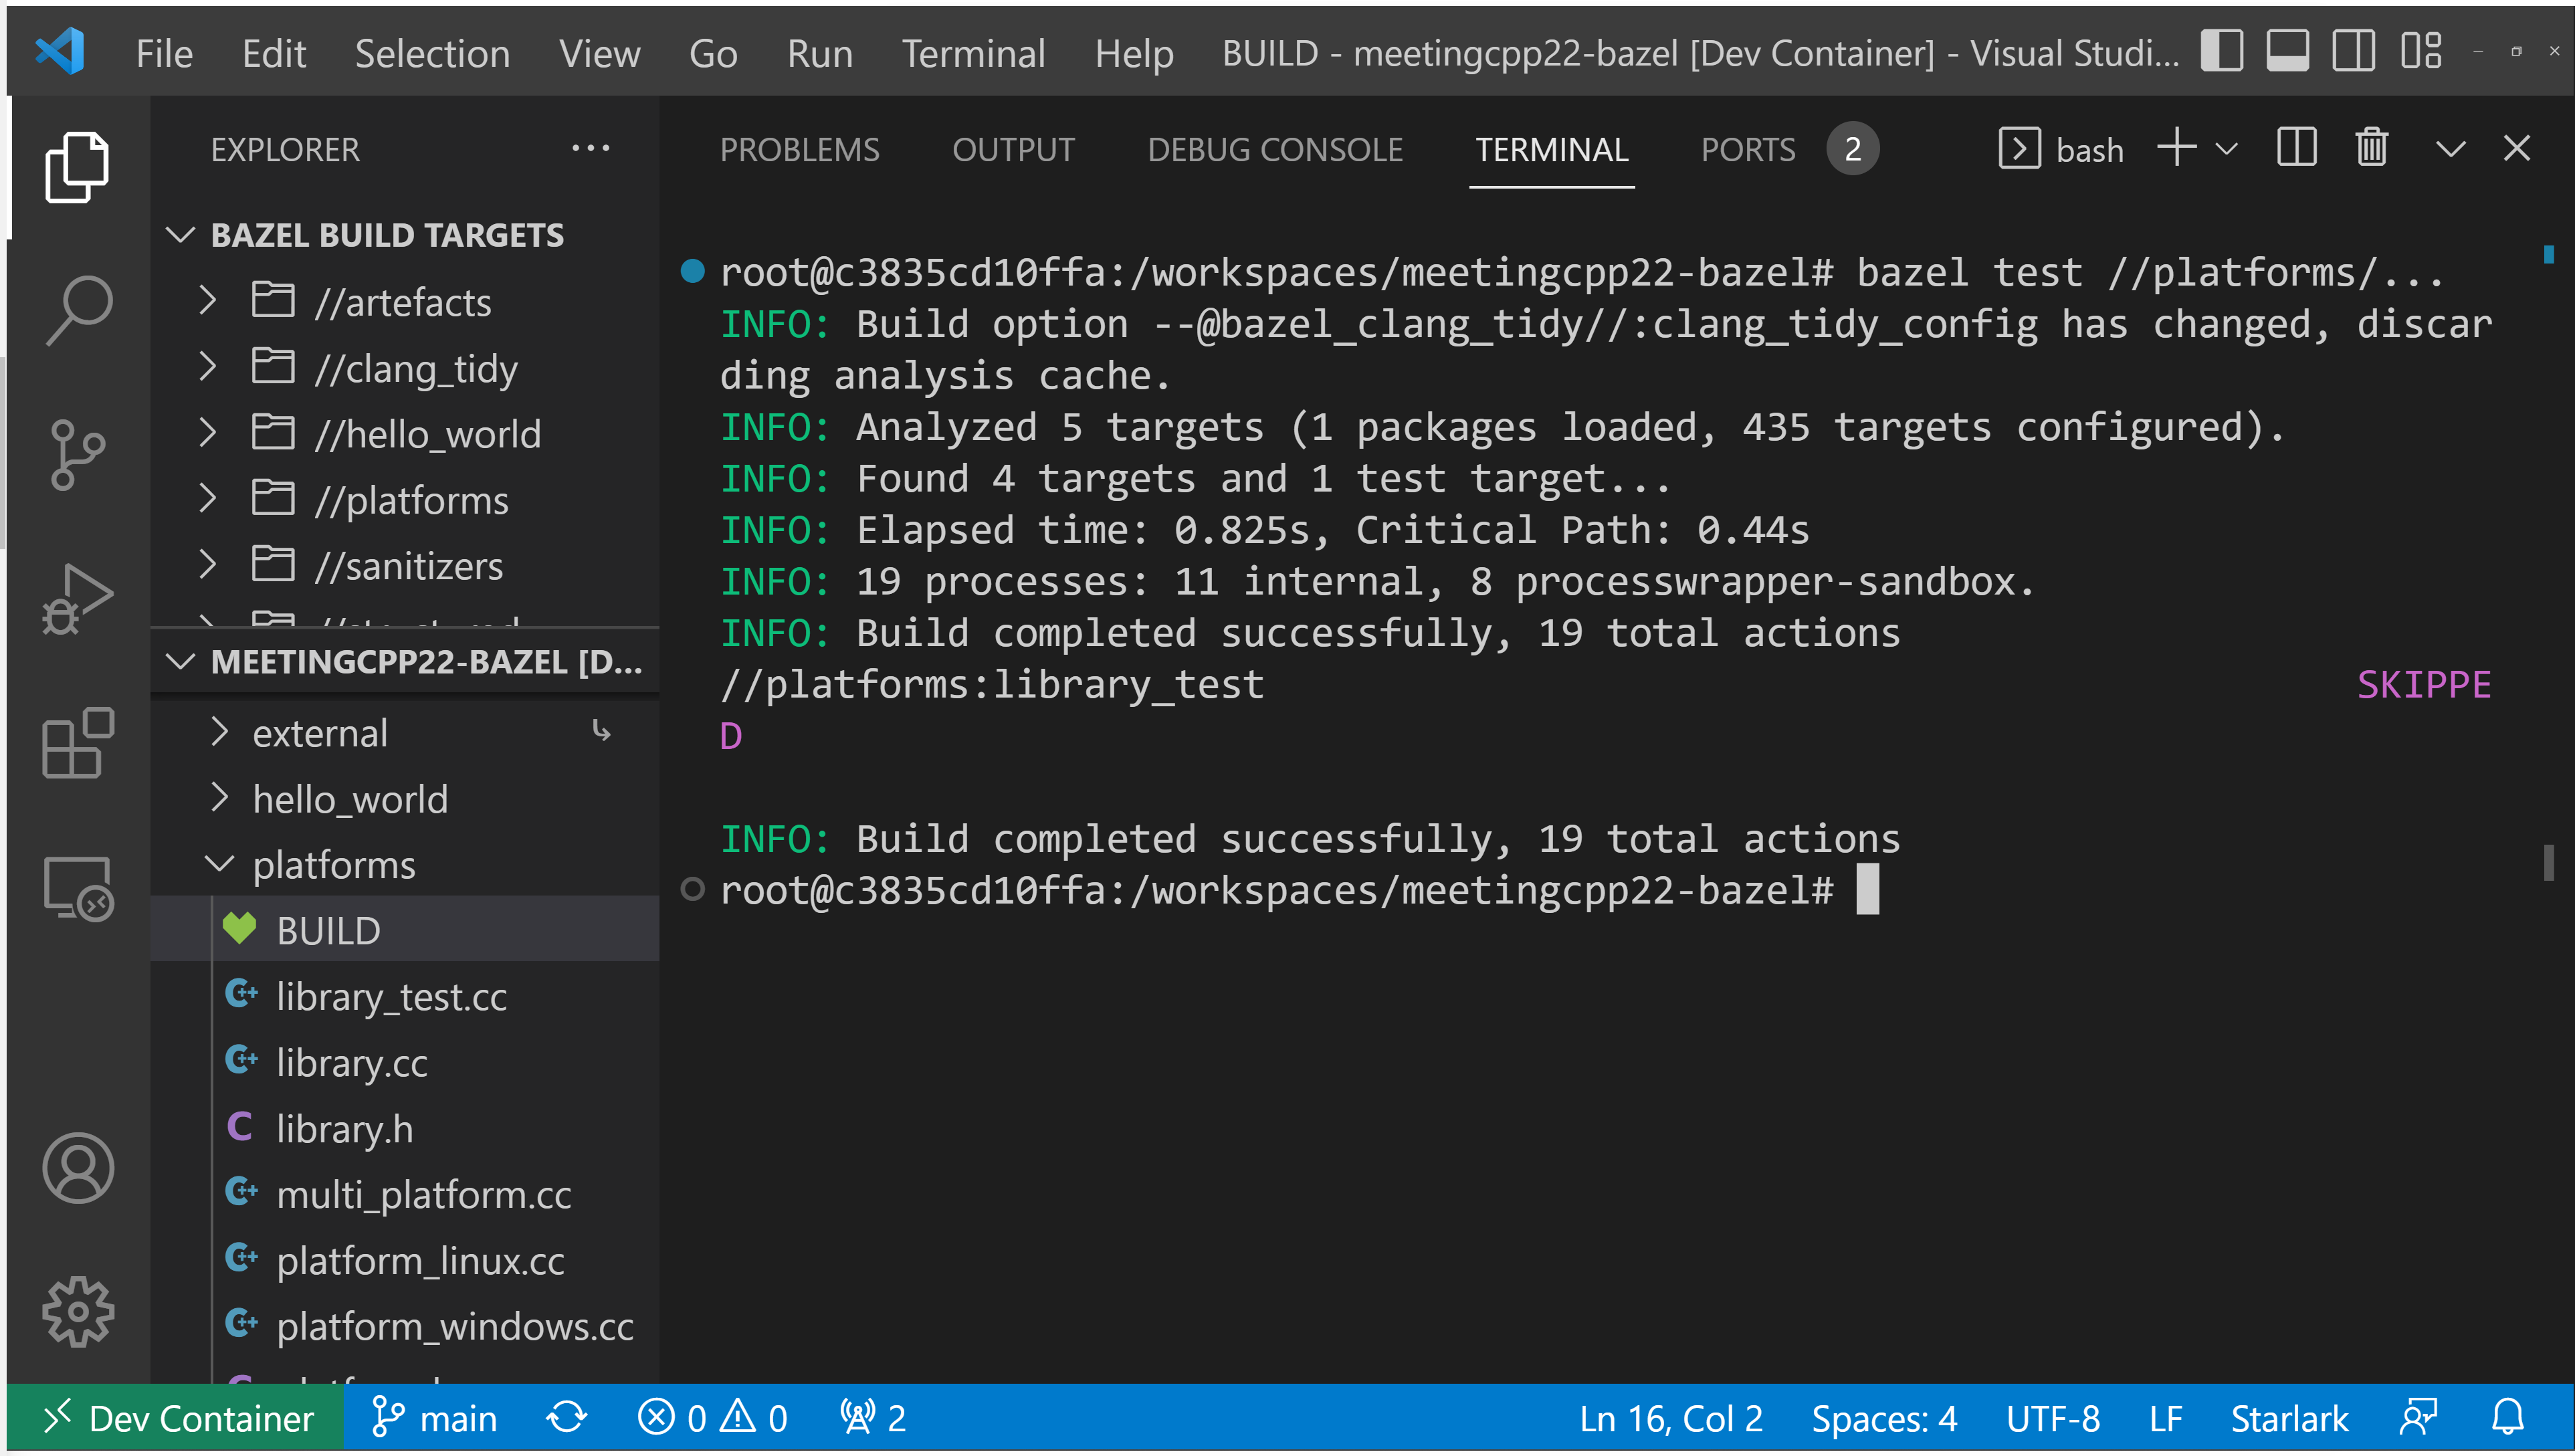
\includegraphics[width=\paperwidth]{slides/static_demos/05_01_skipped.png}}
\begin{frame}[plain]
\end{frame}
}

{
\usebackgroundtemplate{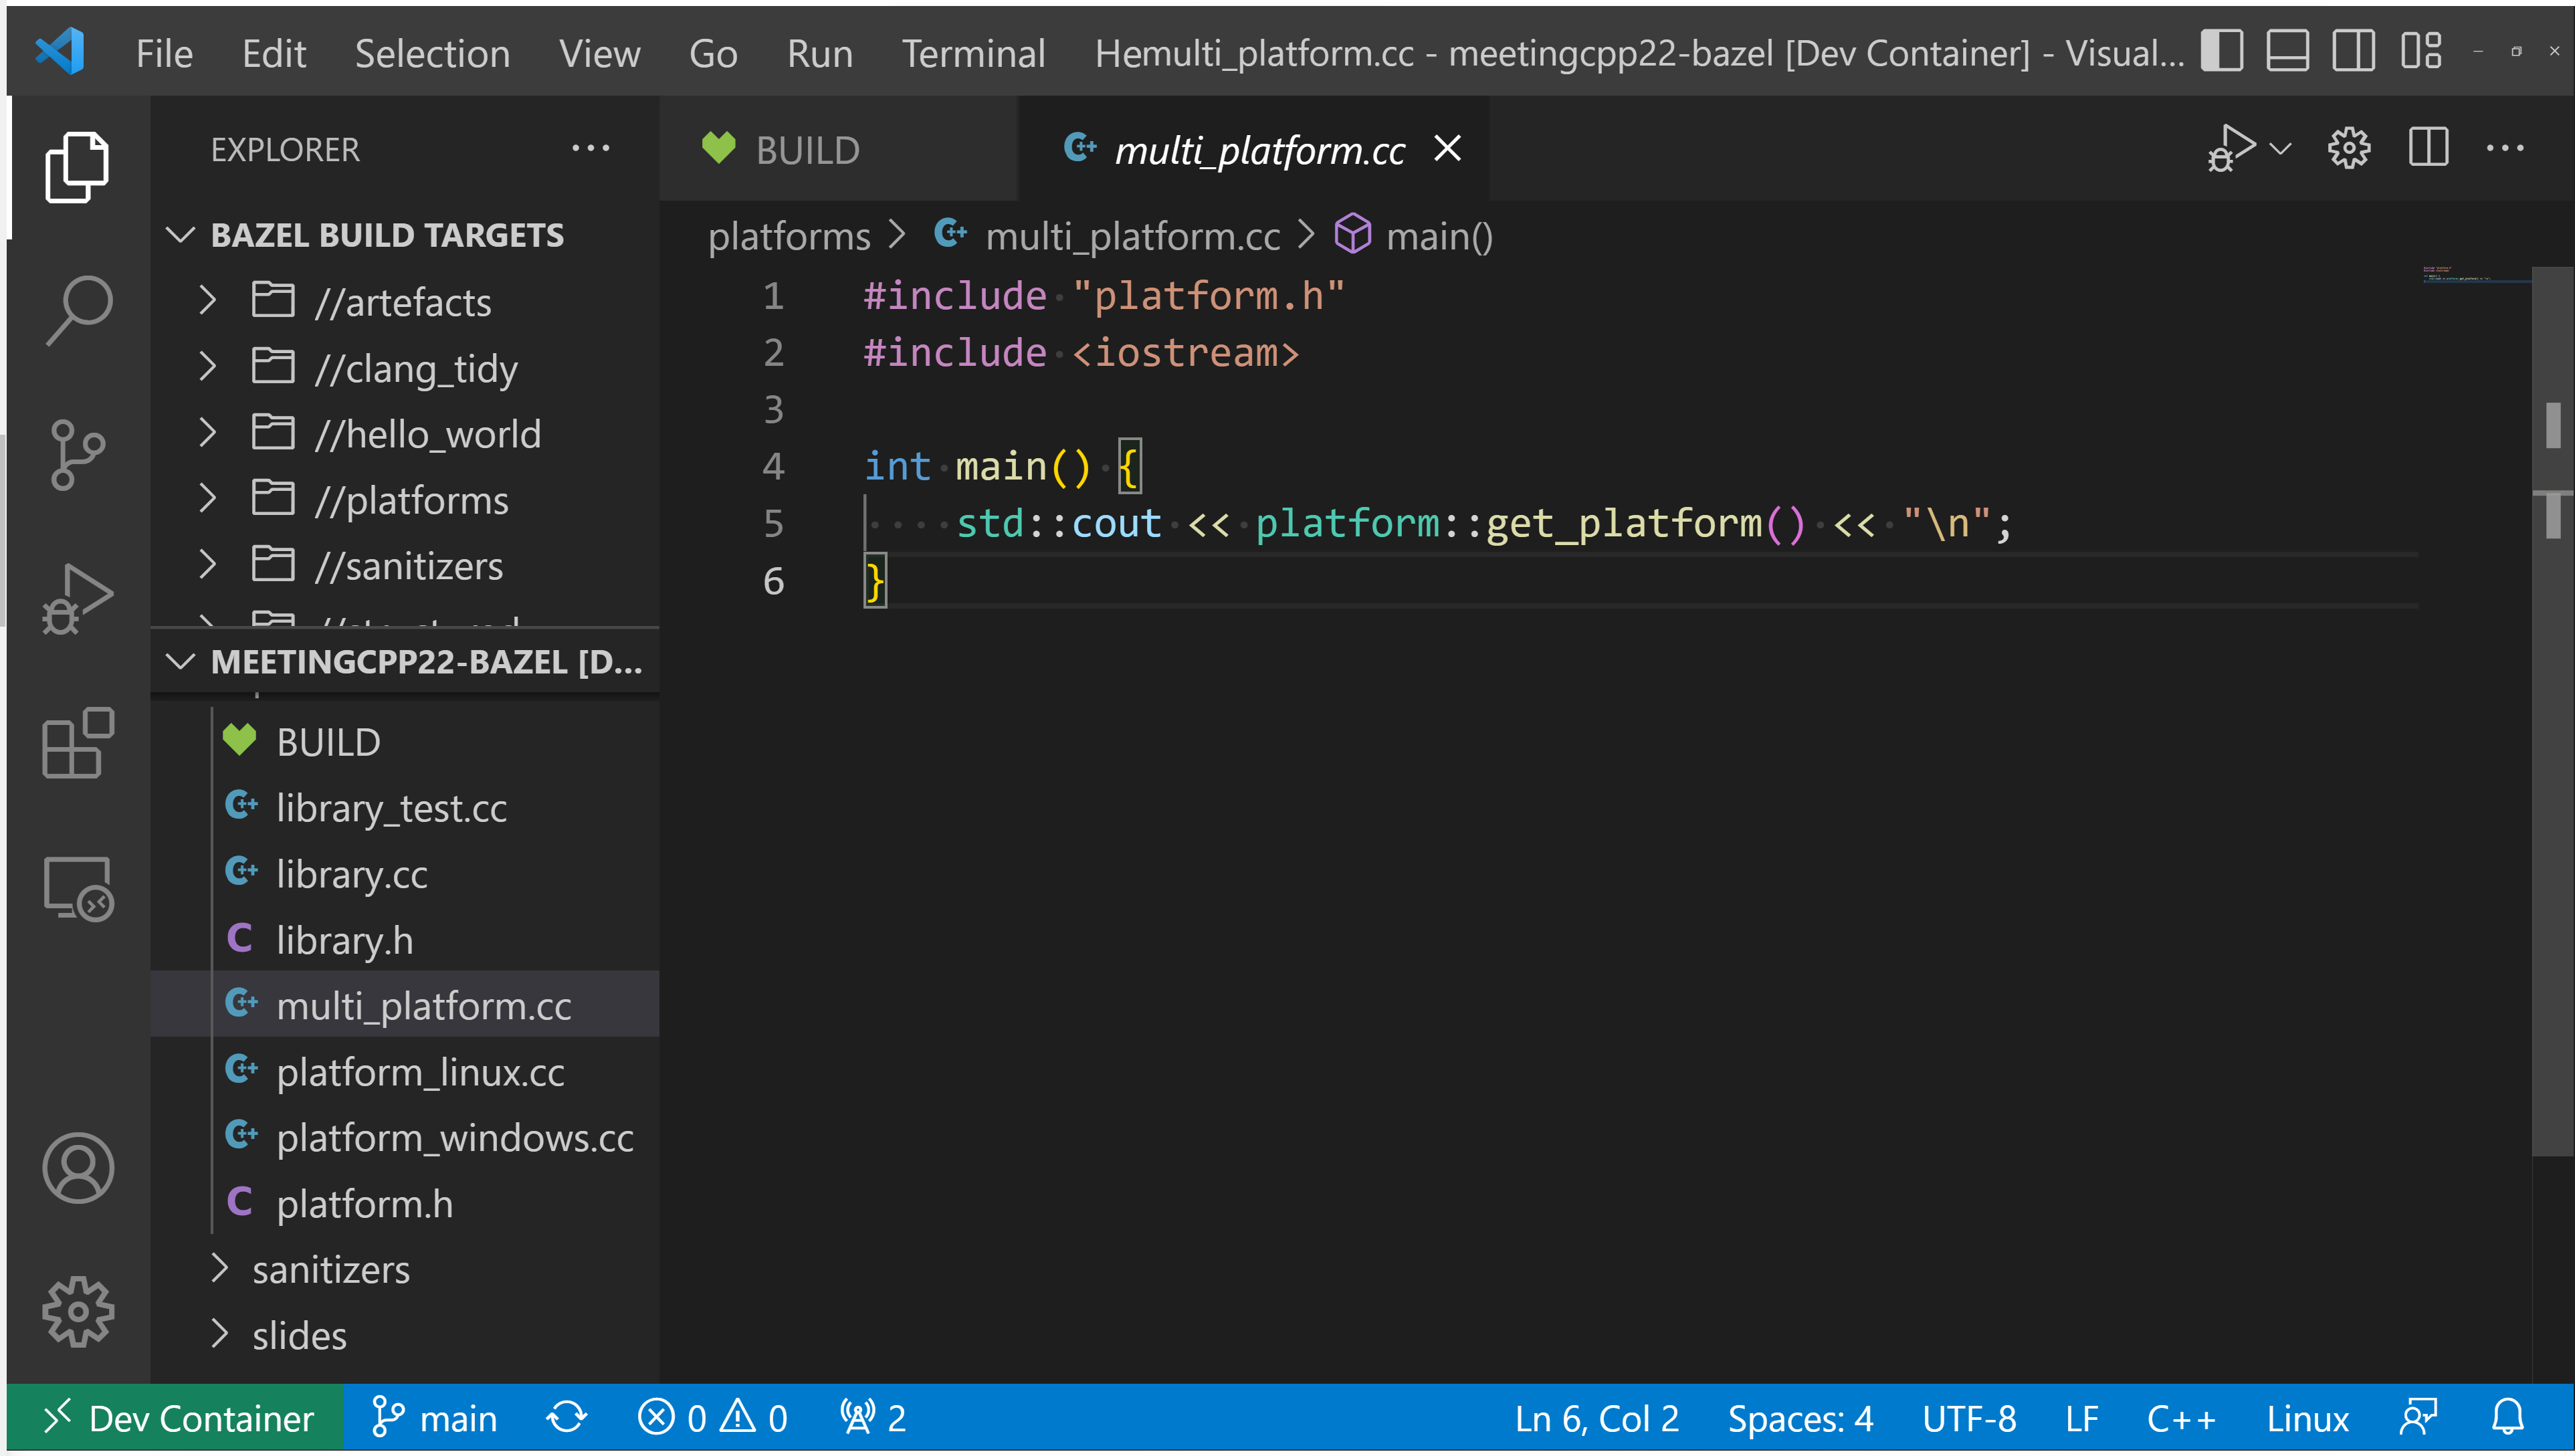
\includegraphics[width=\paperwidth]{slides/static_demos/05_02_src_multi.png}}
\begin{frame}[plain]
\end{frame}
}

{
\usebackgroundtemplate{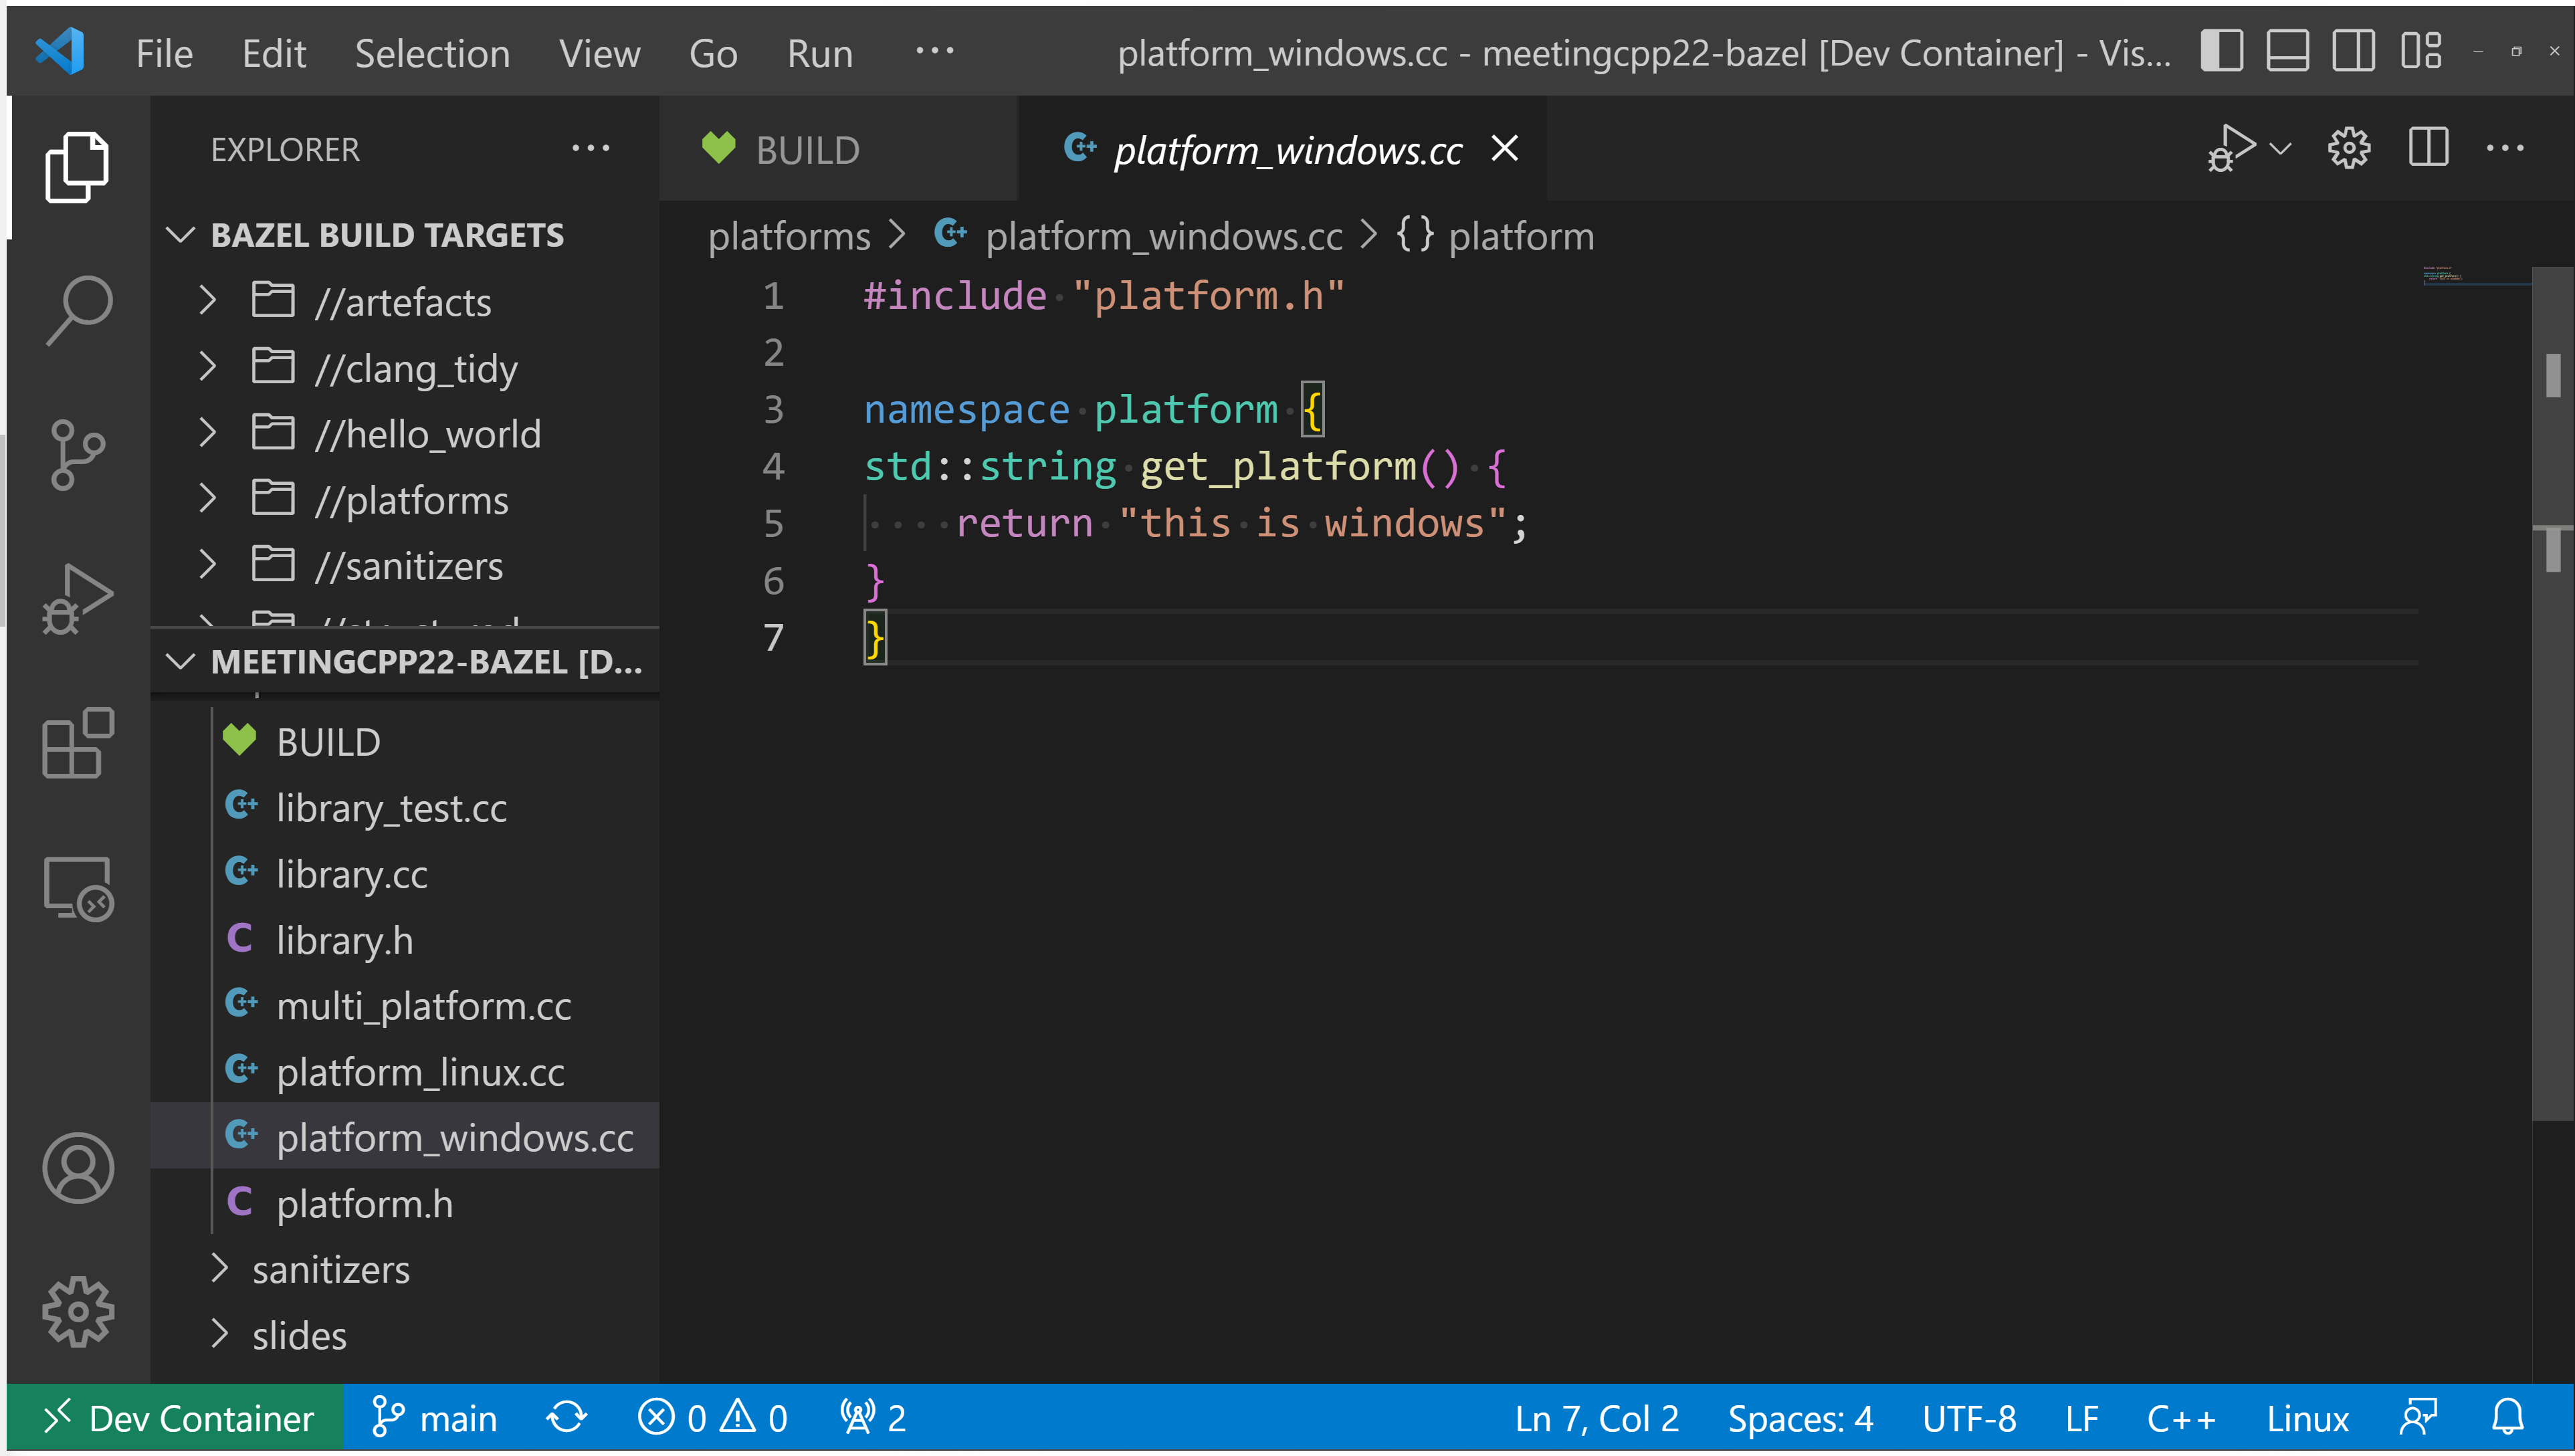
\includegraphics[width=\paperwidth]{slides/static_demos/05_03_src_win.png}}
\begin{frame}[plain]
\end{frame}
}

{
\usebackgroundtemplate{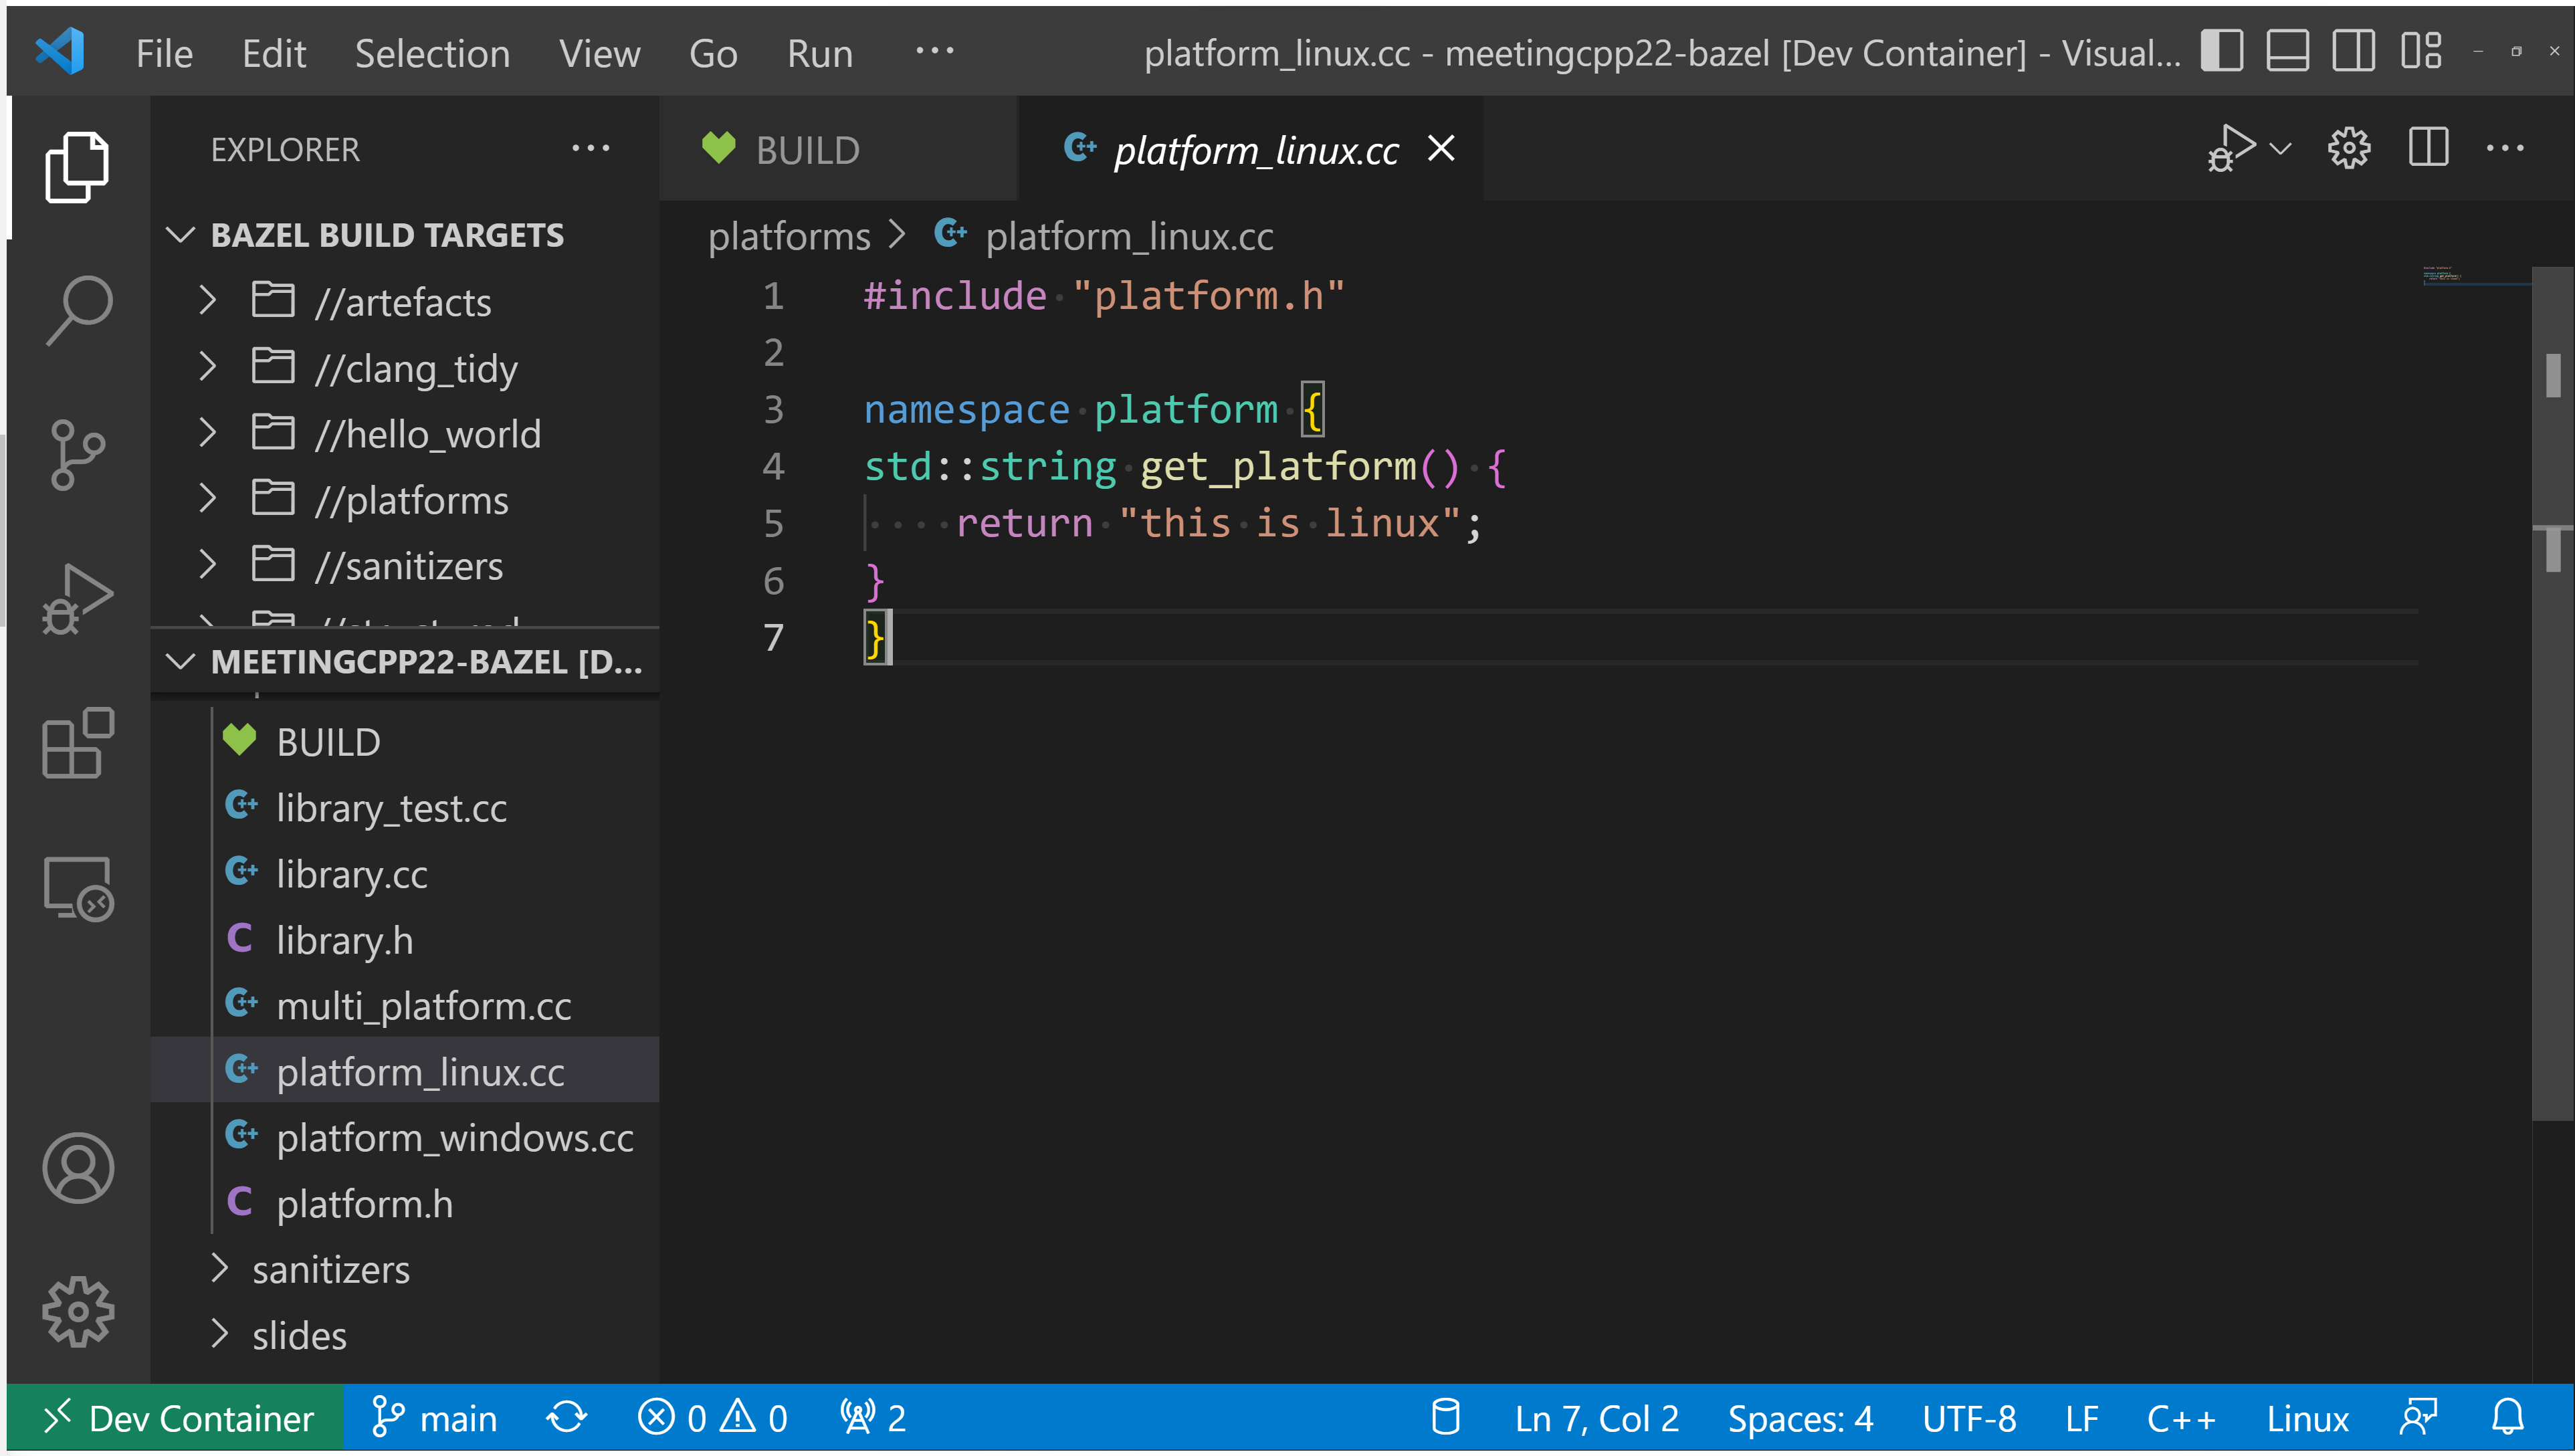
\includegraphics[width=\paperwidth]{slides/static_demos/05_04_src_lin.png}}
\begin{frame}[plain]
\end{frame}
}

{
\usebackgroundtemplate{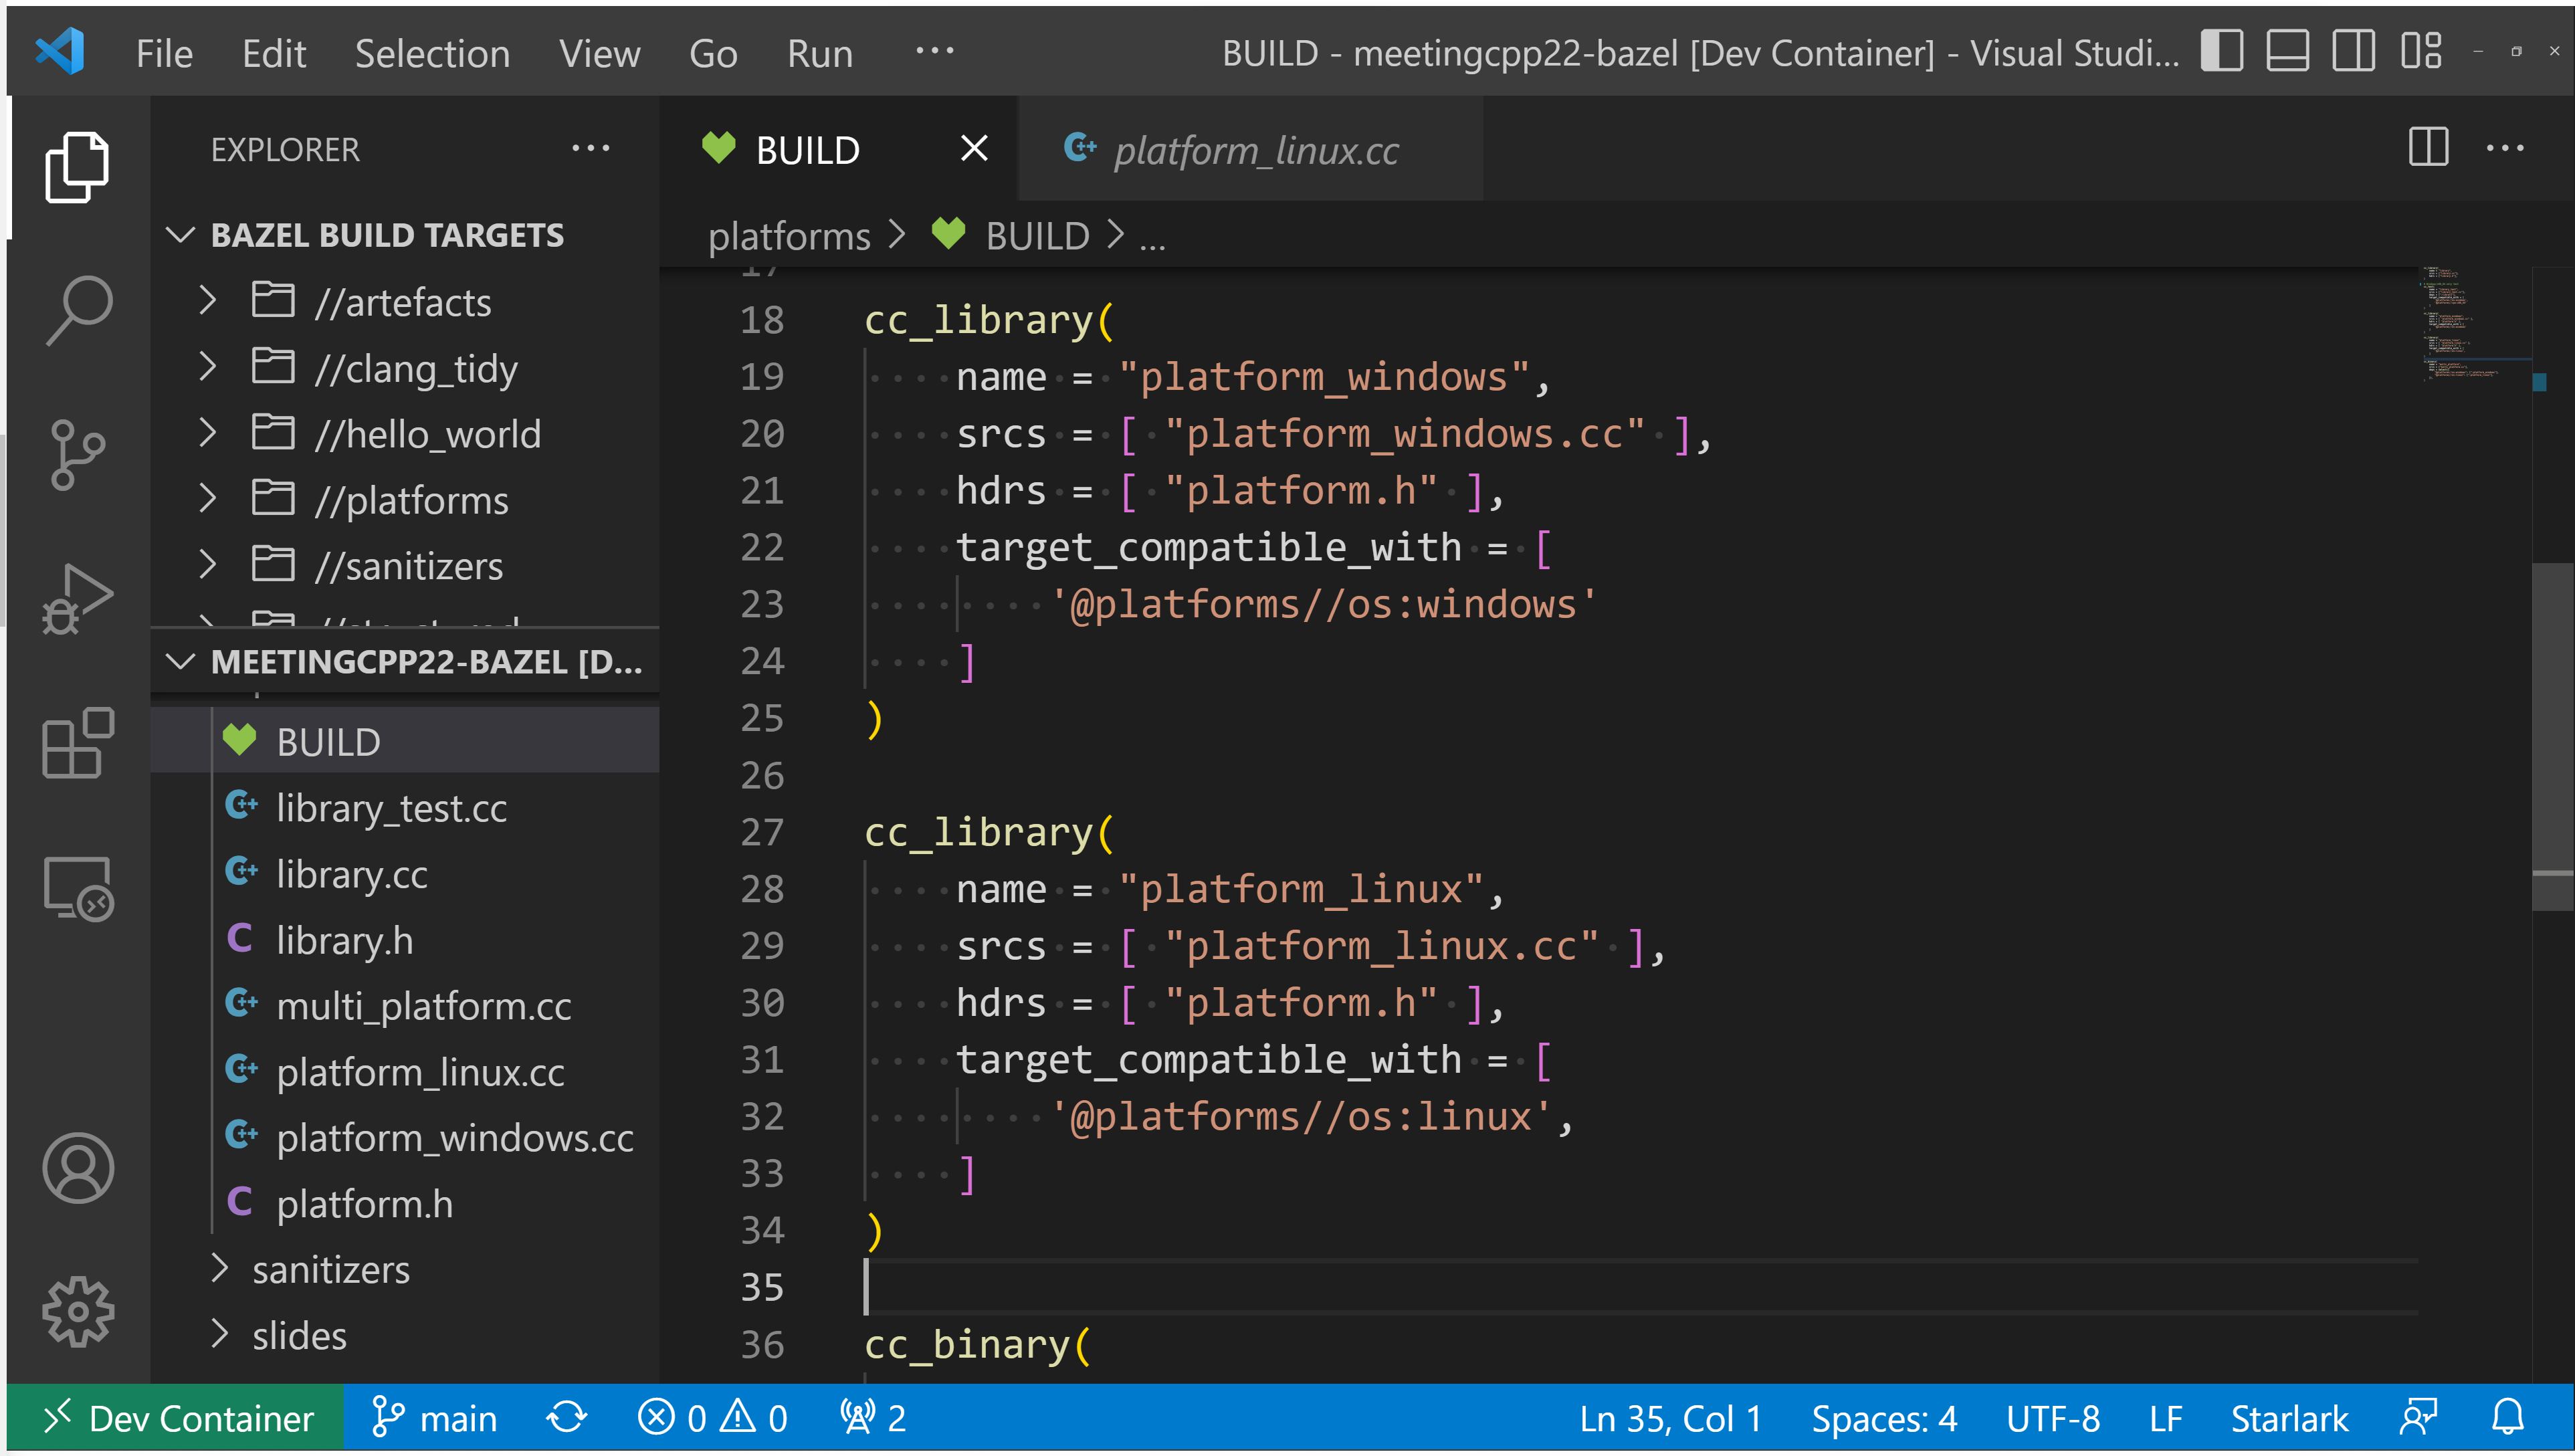
\includegraphics[width=\paperwidth]{slides/static_demos/05_05_build.png}}
\begin{frame}[plain]
\end{frame}
}

{
\usebackgroundtemplate{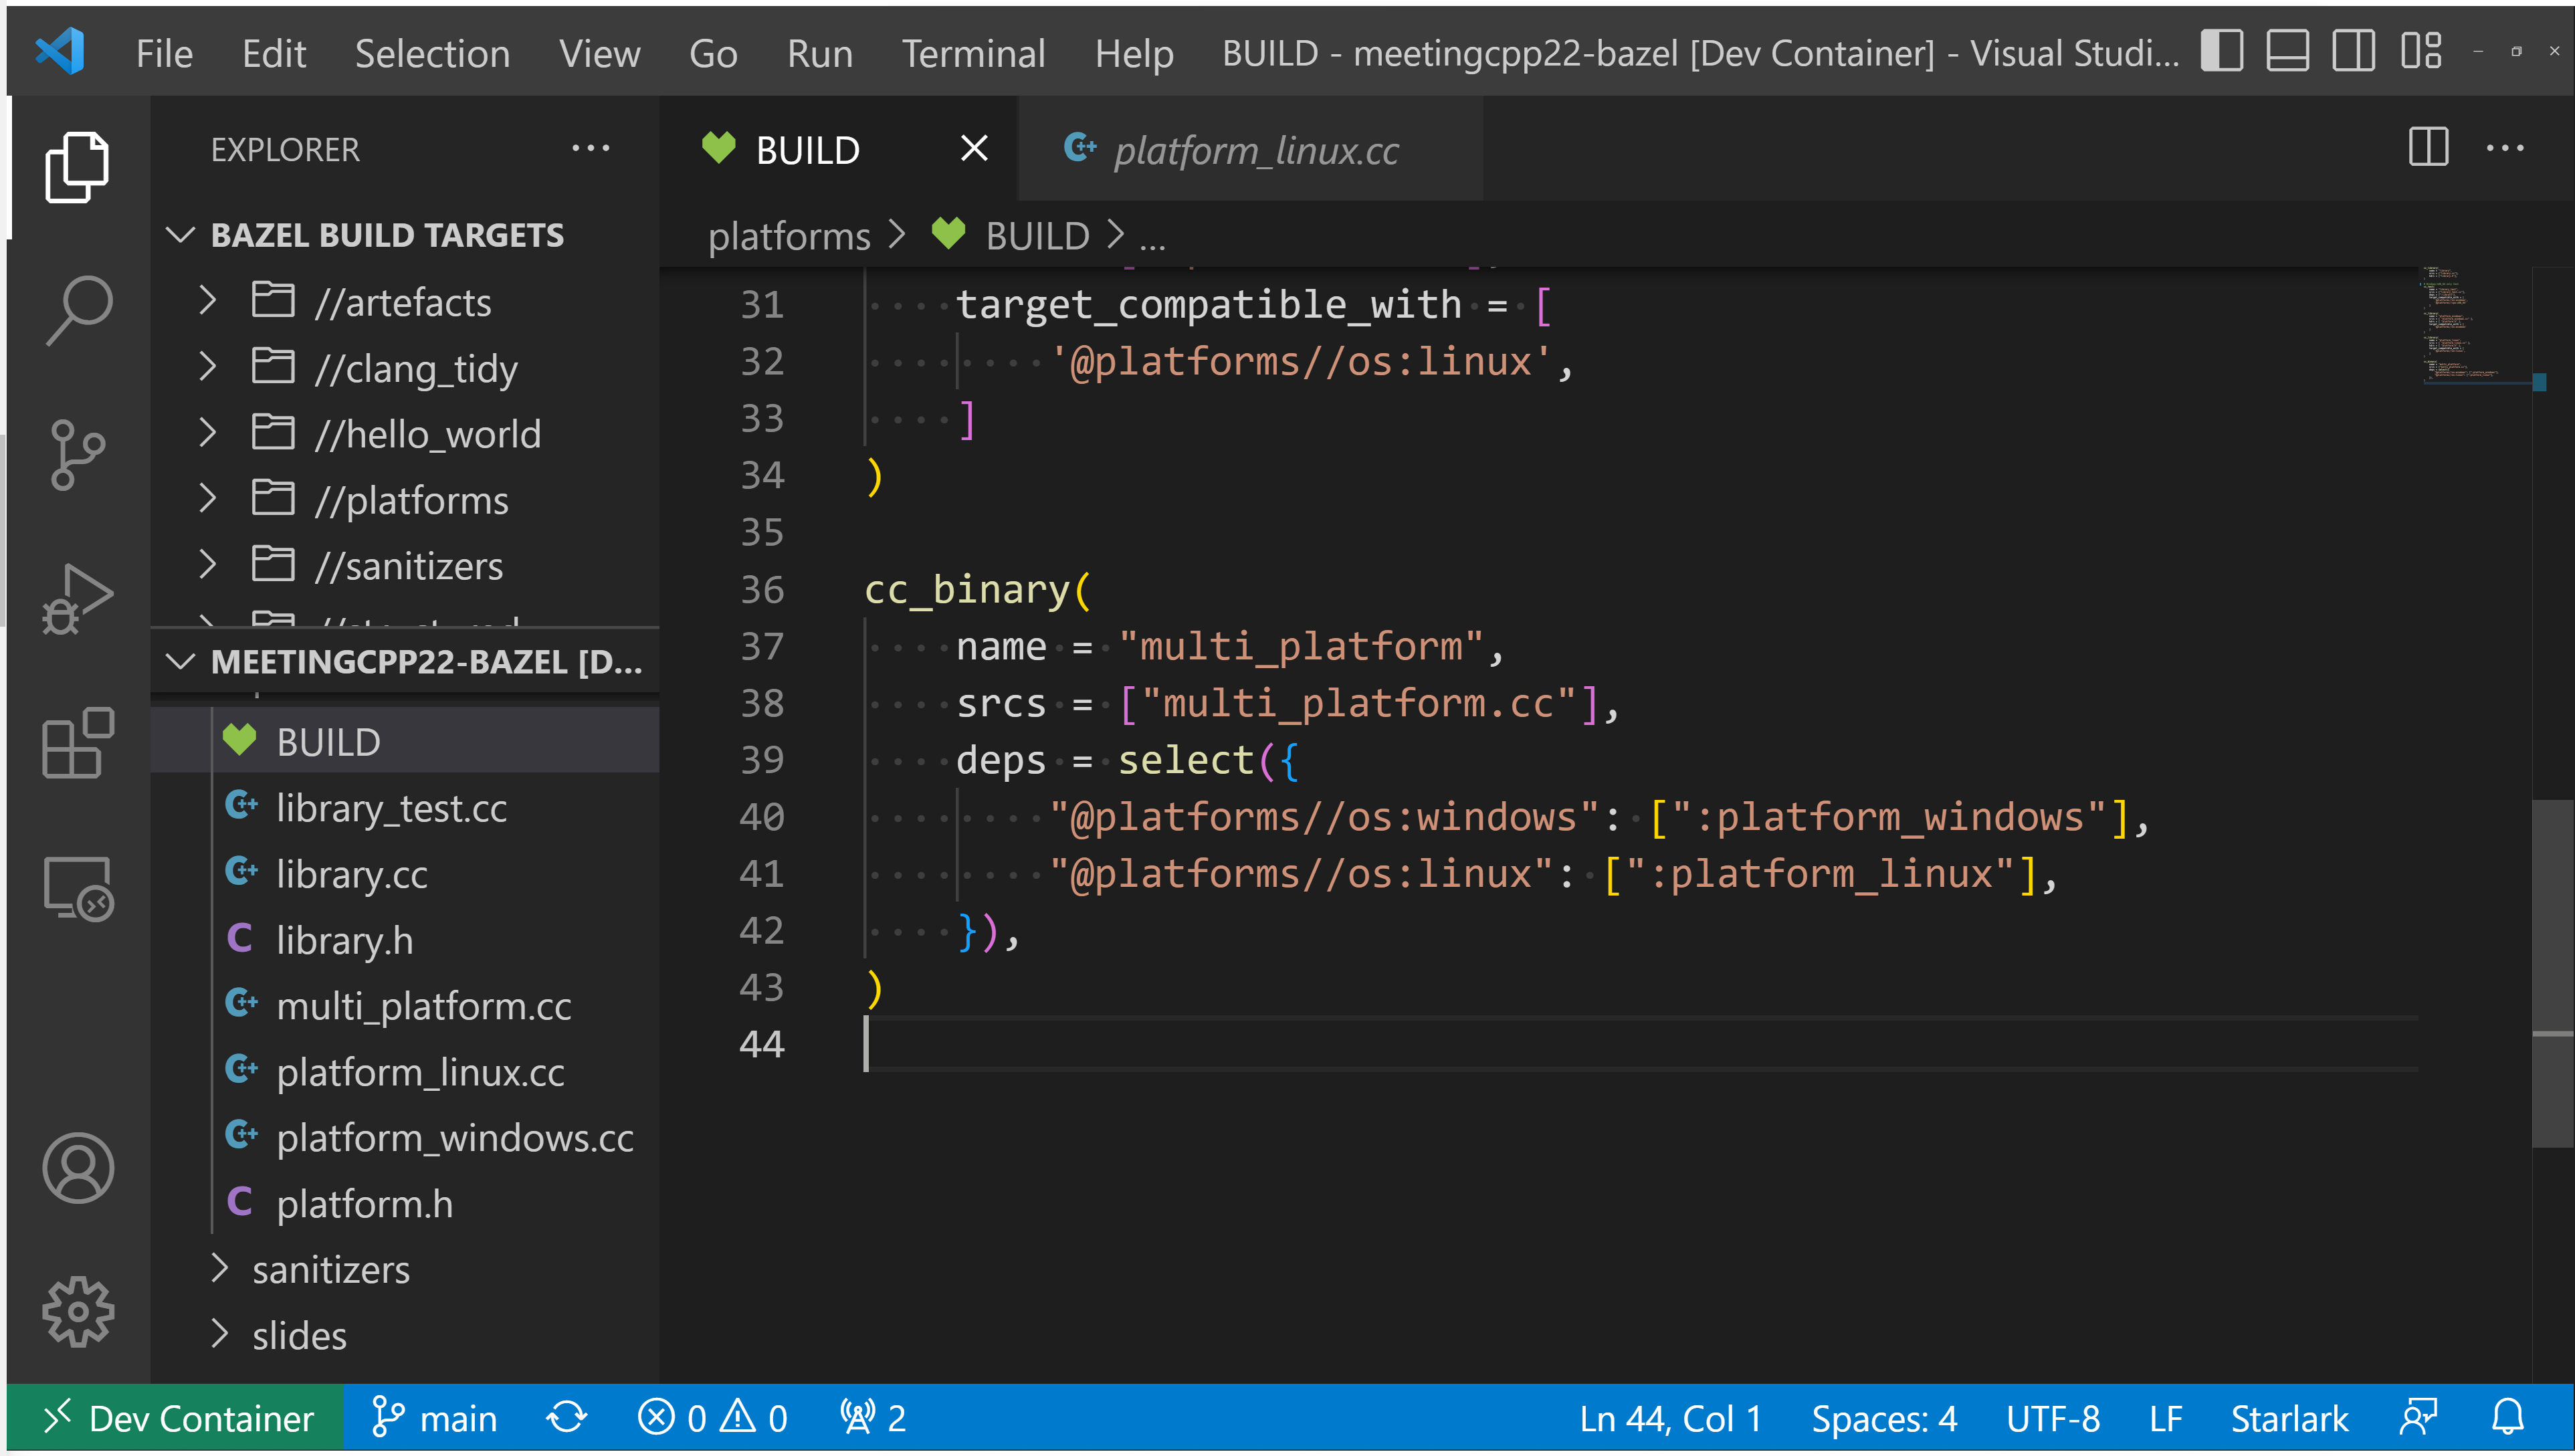
\includegraphics[width=\paperwidth]{slides/static_demos/05_06_build_main.png}}
\begin{frame}[plain]
\end{frame}
}

{
\usebackgroundtemplate{\includegraphics[width=\paperwidth]{slides/static_demos/05_07_run.png}}
\begin{frame}[plain]
\end{frame}
}

\begin{frame}{}
    \begin{center}
        \begin{Huge}Toolchains\end{Huge}
    \end{center}
\end{frame}

{
\usebackgroundtemplate{\includegraphics[width=\paperwidth]{slides/static_demos/06_00_workspace.png}}
\begin{frame}[plain]
\end{frame}
}

{
\usebackgroundtemplate{\includegraphics[width=\paperwidth]{slides/static_demos/06_01_hello_src.png}}
\begin{frame}[plain]
\end{frame}
}

{
\usebackgroundtemplate{\includegraphics[width=\paperwidth]{slides/static_demos/06_02_wasm_rule.png}}
\begin{frame}[plain]
\end{frame}
}

{
\usebackgroundtemplate{\includegraphics[width=\paperwidth]{slides/static_demos/06_03_build.png}}
\begin{frame}[plain]
\end{frame}
}

{
\usebackgroundtemplate{\includegraphics[width=\paperwidth]{slides/static_demos/06_04_run.png}}
\begin{frame}[plain]
\end{frame}
}

\begin{frame}{}
    \begin{center}
        \begin{Huge}Packages\end{Huge}
    \end{center}
\end{frame}

{
\usebackgroundtemplate{\includegraphics[width=\paperwidth]{slides/static_demos/07_00_code.png}}
\begin{frame}[plain]
\end{frame}
}

{
\usebackgroundtemplate{\includegraphics[width=\paperwidth]{slides/static_demos/07_01_pkg_bin.png}}
\begin{frame}[plain]
\end{frame}
}

{
\usebackgroundtemplate{\includegraphics[width=\paperwidth]{slides/static_demos/07_02_pkg_data.png}}
\begin{frame}[plain]
\end{frame}
}

{
\usebackgroundtemplate{\includegraphics[width=\paperwidth]{slides/static_demos/07_03_debian.png}}
\begin{frame}[plain]
\end{frame}
}

{
\usebackgroundtemplate{\includegraphics[width=\paperwidth]{slides/static_demos/07_04_build.png}}
\begin{frame}[plain]
\end{frame}
}

{
\usebackgroundtemplate{\includegraphics[width=\paperwidth]{slides/static_demos/07_05_install.png}}
\begin{frame}[plain]
\end{frame}
}

{
\usebackgroundtemplate{\includegraphics[width=\paperwidth]{slides/static_demos/07_06_run.png}}
\begin{frame}[plain]
\end{frame}
}

\begin{frame}{}
    \begin{center}
        \begin{Huge}GitHub\end{Huge}
    \end{center}
\end{frame}

{
\usebackgroundtemplate{\includegraphics[width=\paperwidth]{slides/static_demos/08_00_action_part1.png}}
\begin{frame}[plain]
\end{frame}
}

{
\usebackgroundtemplate{\includegraphics[width=\paperwidth]{slides/static_demos/08_01_action_part2.png}}
\begin{frame}[plain]
\end{frame}
}

{
\usebackgroundtemplate{\includegraphics[width=\paperwidth]{slides/static_demos/08_02_test.png}}
\begin{frame}[plain]
\end{frame}
}

{
\usebackgroundtemplate{\includegraphics[width=\paperwidth]{slides/static_demos/08_03_cached.png}}
\begin{frame}[plain]
\end{frame}
}

\begin{frame}{}
    \begin{center}
        \begin{Huge}Remote Cache\end{Huge}
    \end{center}
\end{frame}

{
\usebackgroundtemplate{\includegraphics[width=\paperwidth]{slides/static_demos/09_00_install.png}}
\begin{frame}[plain]
\end{frame}
}

{
\usebackgroundtemplate{\includegraphics[width=\paperwidth]{slides/static_demos/09_01_cache.png}}
\begin{frame}[plain]
\end{frame}
}

{
\usebackgroundtemplate{\includegraphics[width=\paperwidth]{slides/static_demos/09_02_precache.png}}
\begin{frame}[plain]
\end{frame}
}

{
\usebackgroundtemplate{\includegraphics[width=\paperwidth]{slides/static_demos/09_03_read_only.png}}
\begin{frame}[plain]
\end{frame}
}

{
\usebackgroundtemplate{\includegraphics[width=\paperwidth]{slides/static_demos/09_04_cached.png}}
\begin{frame}[plain]
\end{frame}
}

\begin{frame}{}
    \begin{center}
        \begin{Huge}Final remarks\end{Huge}
    \end{center}
\end{frame}

\begin{frame}{}
    \begin{center}
        \begin{Huge}Windows support?\end{Huge}\\
        \href{https://bazel.build/configure/windows}{https://bazel.build/configure/windows}
    \end{center}
\end{frame}

\begin{frame}{}
    \begin{center}
        \begin{Huge}Bleeding edge features.\end{Huge}
    \end{center}
\end{frame}

\begin{frame}{}
    \begin{center}
        \begin{Huge}3rd party modules?\end{Huge}
    \end{center}
\end{frame}

\begin{frame}{}
    \begin{center}
        \begin{Huge}C++20 modules?\end{Huge}\\
        \href{https://github.com/rnburn/rules_cc_module}{https://github.com/rnburn/rules\_cc\_module}\\
        \href{https://github.com/eomii/rules_ll}{https://github.com/eomii/rules\_ll}\\
        \textbf{rules\_ll got an update as I was editing this recording a should work!}
\end{center}
\end{frame}

\begin{frame}{}
    \begin{center}
        \begin{Huge}Integration tests?\end{Huge}
    \end{center}
\end{frame}

\begin{frame}{}
    \begin{center}
        \begin{Huge}Dependencies without Bazel support?\end{Huge}\\
        \href{https://github.com/bazelbuild/rules_foreign_cc}{https://github.com/bazelbuild/rules\_foreign\_cc}
    \end{center}
\end{frame}

\begin{frame}{}
    \begin{center}
        \begin{Huge}Living comfortably at HEAD with Bazel\end{Huge}
    \end{center}
\end{frame}

\begin{frame}{}
    \begin{columns}
        \begin{column}{0.27\textwidth}
            \includegraphics[height=0.8\textheight]{static/book_cover.png}
        \end{column}
        \begin{column}{0.43\textwidth}
        \small
            \begin{itemize}
                \item \href{https://github.com/HappyCerberus/book-cpp-algorithms}{HappyCerberus/book-cpp-algorithms}
                \item \href{https://leanpub.com/cpp-algorithms-guide}{leanpub.com/cpp-algorithms-guide}
            \end{itemize}
            \begin{itemize}
                \item \href{https://twitter.com/SimonToth83}{twitter.com/SimonToth83}
                \item \href{https://www.linkedin.com/in/simontoth}{linkedin.com/in/simontoth}
            \end{itemize}
        \end{column}
    \begin{column}{0.3\textwidth}
        \hspace{-1em}\includegraphics[width=1.08\textwidth]{static/tweet.png}
    \end{column}        
    \end{columns}
\end{frame}

\end{document}